% Options for packages loaded elsewhere
\PassOptionsToPackage{unicode}{hyperref}
\PassOptionsToPackage{hyphens}{url}
%
\documentclass[
]{book}
\usepackage{amsmath,amssymb}
\usepackage{iftex}
\ifPDFTeX
  \usepackage[T1]{fontenc}
  \usepackage[utf8]{inputenc}
  \usepackage{textcomp} % provide euro and other symbols
\else % if luatex or xetex
  \usepackage{unicode-math} % this also loads fontspec
  \defaultfontfeatures{Scale=MatchLowercase}
  \defaultfontfeatures[\rmfamily]{Ligatures=TeX,Scale=1}
\fi
\usepackage{lmodern}
\ifPDFTeX\else
  % xetex/luatex font selection
\fi
% Use upquote if available, for straight quotes in verbatim environments
\IfFileExists{upquote.sty}{\usepackage{upquote}}{}
\IfFileExists{microtype.sty}{% use microtype if available
  \usepackage[]{microtype}
  \UseMicrotypeSet[protrusion]{basicmath} % disable protrusion for tt fonts
}{}
\makeatletter
\@ifundefined{KOMAClassName}{% if non-KOMA class
  \IfFileExists{parskip.sty}{%
    \usepackage{parskip}
  }{% else
    \setlength{\parindent}{0pt}
    \setlength{\parskip}{6pt plus 2pt minus 1pt}}
}{% if KOMA class
  \KOMAoptions{parskip=half}}
\makeatother
\usepackage{fancyvrb}
\usepackage{xcolor}
\usepackage{color}
\usepackage{fancyvrb}
\newcommand{\VerbBar}{|}
\newcommand{\VERB}{\Verb[commandchars=\\\{\}]}
\DefineVerbatimEnvironment{Highlighting}{Verbatim}{commandchars=\\\{\}}
% Add ',fontsize=\small' for more characters per line
\usepackage{framed}
\definecolor{shadecolor}{RGB}{248,248,248}
\newenvironment{Shaded}{\begin{snugshade}}{\end{snugshade}}
\newcommand{\AlertTok}[1]{\textcolor[rgb]{0.94,0.16,0.16}{#1}}
\newcommand{\AnnotationTok}[1]{\textcolor[rgb]{0.56,0.35,0.01}{\textbf{\textit{#1}}}}
\newcommand{\AttributeTok}[1]{\textcolor[rgb]{0.13,0.29,0.53}{#1}}
\newcommand{\BaseNTok}[1]{\textcolor[rgb]{0.00,0.00,0.81}{#1}}
\newcommand{\BuiltInTok}[1]{#1}
\newcommand{\CharTok}[1]{\textcolor[rgb]{0.31,0.60,0.02}{#1}}
\newcommand{\CommentTok}[1]{\textcolor[rgb]{0.56,0.35,0.01}{\textit{#1}}}
\newcommand{\CommentVarTok}[1]{\textcolor[rgb]{0.56,0.35,0.01}{\textbf{\textit{#1}}}}
\newcommand{\ConstantTok}[1]{\textcolor[rgb]{0.56,0.35,0.01}{#1}}
\newcommand{\ControlFlowTok}[1]{\textcolor[rgb]{0.13,0.29,0.53}{\textbf{#1}}}
\newcommand{\DataTypeTok}[1]{\textcolor[rgb]{0.13,0.29,0.53}{#1}}
\newcommand{\DecValTok}[1]{\textcolor[rgb]{0.00,0.00,0.81}{#1}}
\newcommand{\DocumentationTok}[1]{\textcolor[rgb]{0.56,0.35,0.01}{\textbf{\textit{#1}}}}
\newcommand{\ErrorTok}[1]{\textcolor[rgb]{0.64,0.00,0.00}{\textbf{#1}}}
\newcommand{\ExtensionTok}[1]{#1}
\newcommand{\FloatTok}[1]{\textcolor[rgb]{0.00,0.00,0.81}{#1}}
\newcommand{\FunctionTok}[1]{\textcolor[rgb]{0.13,0.29,0.53}{\textbf{#1}}}
\newcommand{\ImportTok}[1]{#1}
\newcommand{\InformationTok}[1]{\textcolor[rgb]{0.56,0.35,0.01}{\textbf{\textit{#1}}}}
\newcommand{\KeywordTok}[1]{\textcolor[rgb]{0.13,0.29,0.53}{\textbf{#1}}}
\newcommand{\NormalTok}[1]{#1}
\newcommand{\OperatorTok}[1]{\textcolor[rgb]{0.81,0.36,0.00}{\textbf{#1}}}
\newcommand{\OtherTok}[1]{\textcolor[rgb]{0.56,0.35,0.01}{#1}}
\newcommand{\PreprocessorTok}[1]{\textcolor[rgb]{0.56,0.35,0.01}{\textit{#1}}}
\newcommand{\RegionMarkerTok}[1]{#1}
\newcommand{\SpecialCharTok}[1]{\textcolor[rgb]{0.81,0.36,0.00}{\textbf{#1}}}
\newcommand{\SpecialStringTok}[1]{\textcolor[rgb]{0.31,0.60,0.02}{#1}}
\newcommand{\StringTok}[1]{\textcolor[rgb]{0.31,0.60,0.02}{#1}}
\newcommand{\VariableTok}[1]{\textcolor[rgb]{0.00,0.00,0.00}{#1}}
\newcommand{\VerbatimStringTok}[1]{\textcolor[rgb]{0.31,0.60,0.02}{#1}}
\newcommand{\WarningTok}[1]{\textcolor[rgb]{0.56,0.35,0.01}{\textbf{\textit{#1}}}}
\usepackage{longtable,booktabs,array}
\usepackage{calc} % for calculating minipage widths
% Correct order of tables after \paragraph or \subparagraph
\usepackage{etoolbox}
\makeatletter
\patchcmd\longtable{\par}{\if@noskipsec\mbox{}\fi\par}{}{}
\makeatother
% Allow footnotes in longtable head/foot
\IfFileExists{footnotehyper.sty}{\usepackage{footnotehyper}}{\usepackage{footnote}}
\makesavenoteenv{longtable}
\usepackage{graphicx}
\makeatletter
\def\maxwidth{\ifdim\Gin@nat@width>\linewidth\linewidth\else\Gin@nat@width\fi}
\def\maxheight{\ifdim\Gin@nat@height>\textheight\textheight\else\Gin@nat@height\fi}
\makeatother
% Scale images if necessary, so that they will not overflow the page
% margins by default, and it is still possible to overwrite the defaults
% using explicit options in \includegraphics[width, height, ...]{}
\setkeys{Gin}{width=\maxwidth,height=\maxheight,keepaspectratio}
% Set default figure placement to htbp
\makeatletter
\def\fps@figure{htbp}
\makeatother
\setlength{\emergencystretch}{3em} % prevent overfull lines
\providecommand{\tightlist}{%
  \setlength{\itemsep}{0pt}\setlength{\parskip}{0pt}}
\setcounter{secnumdepth}{5}
\usepackage{booktabs}
\usepackage{amsthm}
\makeatletter
\def\thm@space@setup{%
  \thm@preskip=8pt plus 2pt minus 4pt
  \thm@postskip=\thm@preskip
}
\makeatother

% Added by Miratrix
\usepackage{color}
\newcommand\cmnt[2]{\qquad{{\color{red} \em #1---#2} \qquad}}
\newcommand\cmntM[1]{\cmnt{#1}{Miratrix}}
\newcommand\awk{{{\color{red} {$\leftarrow$ Awkward phrasing}}\qquad}}
\newcommand\cmntMp[1]{{\color{red} $\leftarrow$ {\em #1 -Miratrix} \qquad}}

\ifLuaTeX
  \usepackage{selnolig}  % disable illegal ligatures
\fi
\usepackage[]{natbib}
\bibliographystyle{apalike}
\usepackage{bookmark}
\IfFileExists{xurl.sty}{\usepackage{xurl}}{} % add URL line breaks if available
\urlstyle{same}
\VerbatimFootnotes % allow verbatim text in footnotes
\hypersetup{
  pdftitle={Designing Monte Carlo Simulations in R},
  pdfauthor={Luke W. Miratrix and James E. Pustejovsky (Equal authors)},
  hidelinks,
  pdfcreator={LaTeX via pandoc}}

\title{Designing Monte Carlo Simulations in R}
\author{Luke W. Miratrix and James E. Pustejovsky
(Equal authors)}
\date{2024-07-02}

\begin{document}
\maketitle

{
\setcounter{tocdepth}{1}
\tableofcontents
}
\chapter*{Welcome}\label{welcome}
\addcontentsline{toc}{chapter}{Welcome}

Monte Carlo simulations are a computational technique for investigating how well something works, or for investigating what might happen in a given circumstance.
When we write a simulation, we are able to control how data are generated, which means we can know what the ``right answer'' is.
Then, by repeatedly generating data and then applying some statistical method that data, we can assess how well a statistical method works in practice.

Monte Carlo simulations are an essential tool of inquiry for quantitative methodologists and students of statistics, useful both for small-scale or informal investigations and for formal methodological research.
Despite the ubiquity of simulation work, most quantitative researchers get little formal training in the design and implementation of Monte Carlo simulations. As a result, the simulation studies presented in academic journal articles are highly variable in terms of their high-level logic, scope, programming, and presentation.
Although there has long been discussion of simulation design and implementation among statisticians and methodologists, the available guidance is scattered across many different disciplines, and much of it is focused on mechanics and computing tools, rather than on principles.

In this monograph, we aim to provide an introduction to the logic and mechanics of designing simulation studies, using the R programming language.
Our focus is on simulation studies for formal research purposes (i.e., as might appear in a journal article or dissertation) and for informing the design of empirical studies (e.g., power analysis).
That being said, the ideas of simulation are used in many different contexts and for many different problems, and we believe the overall concepts illustrated by these ``conventional'' simulations readily carry over into all sorts of other types of use, even statistical inference!
Our focus is on the best practices of simulation design and how to use simulation to be a more informed and effective quantitative analyst.
In particular, we try to provide a guide to designing simulation studies to answer questions about statistical methodology.

Mainly, this book gives practical tools (i.e., lots of code to simply take and repurpose) along with some thoughts and guidance for writing simulations.
We hope you find it to be a useful handbook to help you with your own projects, whatever they happen to be!

\section*{License}\label{license}
\addcontentsline{toc}{section}{License}

This book is licensed to you under \href{http://creativecommons.org/licenses/by-nc-nd/4.0/}{Creative Commons Attribution-NonCommercial-NoDerivatives 4.0 International License}.

The code samples in this book are licensed under \href{https://creativecommons.org/publicdomain/zero/1.0/}{Creative Commons CC0 1.0 Universal (CC0 1.0)}, i.e.~public domain.

\section*{About the authors}\label{about-the-authors}
\addcontentsline{toc}{section}{About the authors}

We wrote this book in full collaboration, because we thought it would be fun to have some reason to talk about how to write simulations, and we wanted more people to be writing high-quality simulations.
Our author order is alphabetical, but perhaps imagine it as a circle, or something with no start or end:

\begin{center}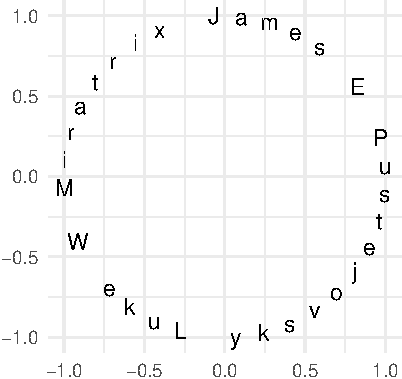
\includegraphics[width=0.75\linewidth]{Designing-Simulations-in-R_files/figure-latex/unnamed-chunk-2-1} \end{center}

But anymore, more about us.

\textbf{James E. Pustejovsky} is an associate professor at the University of Wisconsin - Madison, where he teaches in the Quantitative Methods Program within the Department of Educational Psychology. He completed a Ph.D.~in Statistics at Northwestern University.

\textbf{Luke Miratrix}: I am currently an associate professor at Harvard University's Graduate School of Education. I completed a Ph.D.~in Statistics at UC Berkeley after having traveled through three different graduate programs (computer science at MIT, education at UC Berkeley, and then finally statistics at UC Berkeley).
I then ended up as an assistant professor in Harvard's statistics department, and moved (back) to Education a few years later.

Over the years, simulation has become a way for me to think.
This might be because I am fundamentally lazy, and the idea of sitting down and trying to do a bunch of math to figure something out seems less fun than writing up some code ``real quick'' so I can see how things operate. Of course, ``real quick'' rarely is that quick -- and before I know it I got sucked into trying to learn some esoteric aspect of how to best program something, and then a few rabbit holes later I may have discovered something interesting! I find simulation quite absorbing, and I also find them reassuring (usually with regards to whether I have correctly implemented some statistical method). This book has been a real pleasure to write, because it's given me actual license to sit down and think about why I do the various things I do, and also which way I actually prefer to approach a problem. And getting to write this book with my co-author has been a particular pleasure, for talking about the business of writing simulations is rarely done in practice. This has been a real gift, and I have learned so much.

\section*{Acknowledgements}\label{acknowledgements}
\addcontentsline{toc}{section}{Acknowledgements}

The material in this book was initially developed through courses that we offered at the University of Texas at Austin (James) and Harvard University (Luke) as well as from a series of workshops that we offered through the Society for Research on Educational Effectiveness in June of 2021. We are grateful for feedback, questions, and corrections we have received from many students who participated in these courses. Some parts of this book are based on memos or other writings generated for various purposes, some of which were written by others. This is been attributed throughout.

\part{An Introductory Look}\label{part-an-introductory-look}

\chapter{Introduction}\label{introduction}

Monte Carlo simulations are computational experiments that involve using random number generators to study the behavior of statistical or mathematical models.
Monte Carlo studies are an essential tool in many different fields of science---ranging from climate science to education research---and are used for a variety of different purposes.
Simulations are used to model complex stochastic processes such as weather patterns \citep{jones2012IntroductionScientificProgramming, robert2010IntroducingMonteCarlo};
to generate parameter estimates from complex statistical models, as in Markov Chain Monte Carlo sampling \citep{gelman2013BayesianDataAnalysis};
and even to uncertainty in statistical summaries, as in bootstrapping \citep{davison1997BootstrapMethodsTheir}.
Within the fields of statistics and quantitative methodology, simulation studies play a critical role in the development and validation of methods for data analysis.
In this book, we will examine the use of simulation for this last purpose of using Monte Carlo simulation methods to understand the properties of data analysis methods.

Within quantitatively oriented fields, researchers developing new statistical methods or evaluating the use of existing methods nearly always use Monte Carlo simulations as part of their research process.
In this context, researchers use simulations in a way analogous to how a chef would use their test kitchen to develop new recipes before putting them on the menu, how a manufacturer would use a materials testing laboratory to evaluate the safety and durability of a new consumer good before bringing it to market, or how an astronaut would prepare for a spacewalk by practicing the process in an underwater mock-up.
Likewise, simulation studies provide a clean and controlled environment for testing out data analysis approaches before putting them to use with real empirical data.

At a very high level, Monte Carlo simulation provides a method for understanding the performance of a statistical model or data analysis method under conditions where the truth is known and can be controlled.
The basic approach for doing so is as follows:

\begin{enumerate}
\def\labelenumi{\arabic{enumi}.}
\tightlist
\item
  Create artificial data using random number generators based on a specific statistical model, or more generally, a \emph{data-generating process}.
\item
  Apply one or more data-analysis procedures, such as estimating a particular statistical model, to the artificial data. (This might be something as simple as calculating a difference in sample means, or it might be an involved, multi-step procedure involving cleansing the data of apparent outliers, imputing missing values, applying a machine-learning algorithm, and carrying out further calculations on the predictions of the algorithm.)
\item
  Repeat Steps 1 and 2 many times.
\item
  Summarize the results across these repetitions in order to understand the general trends or patterns in how the method works.
\end{enumerate}

This approach is useful because one can control the data-generating process and therefore fully know the truth---something that is almost always uncertain when analyzing real, empirical data.
Having full control of the data-generating process makes it possible to assess how well a procedure works by comparing the estimates produced by the data analysis procedure against the true value from the data-generating process.
For instance, one can see if estimates from a statistical procedure are consistently too high or too low;
in simulations that involve more than one data-analysis procedure, one can compare the degree of error in each set of results and determine which procedure is more accurate.

\section{Some of simulation's many uses}\label{some-of-simulations-many-uses}

Monte Carlo simulations allow for rapid exploration of different data analysis procedures and, even more broadly, different approaches to designing studies and collecting measurements. Simulations are especially useful because they provide a means to answer questions that are difficult or impossible to answer by other means.
Many statistical models and estimation methods \emph{can} be analyzed mathematically, but only by using asymptotic approximations that describe how the methods work as the sample sizes increases towards infinity.
In contrast, simulation methods provide answers for specific, finite sample sizes.
Thus, they allow researchers to study models and estimation methods where relevant algebraic formulas are not available, not easily applied, or not sufficiently accurate.

Circumstances where simulations are helpful---or even essential---occur in a range of different situations within quantitative research.
To set the stage for our subsequent presentation, consider the following areas where one might find need of simulation.

\subsection{Comparing statistical approaches}\label{comparing-statistical-approaches}

Perhaps one of the most common uses of Monte Carlo simulation is to compare alternative statistical approaches to analyzing the same type of data.
In the academic literature on statistical methodology, authors frequently report simulation studies comparing a newly proposed method against more traditional approaches, to make a case for the utility of their method.
A classic example of such work is \citet{brown1974SmallSampleBehavior}, who compared four different procedures for conducting a hypothesis test for equality of means in several populations (i.e., one-way ANOVA) when the population variances are not equal.
A subsequent study by \citet{mehrotra1997ImprovingBrownforsytheSolution} built on Brown and Forsythe's work, proposing a more refined method and using simulations to demonstrate that it is superior to the existing methods.
We revisit the \citet{brown1974SmallSampleBehavior} example in Chapter \ref{case-ANOVA}.

Comparative simulation can also have a practical application: In many situations, more than one approach or data analysis methods is possible for addressing a given research question (or estimating a specified target parameter).
Simulations comparing the costs of multiple approaches can be quite informative and can help to guide the design of analytic plans (such as plans included in pre-registered study protocols).
As an example of the type of questions that researchers might encounter in designing analytic plans: what are the practical benefits and costs of using a model that allows for cross-site impact variation for a multi-site trial \citep{miratrix2021applied}?
In the ideal case, simulations can identify best practices for how to approach analysis of a certain type of data and can surface trade-offs between competing approaches that occur in practice.

\subsection{Assessing performance of complex pipelines}\label{assessing-performance-of-complex-pipelines}

In practice, statistical methods are often used in as part of a multi-step workflow.
For instance, in a regression model, one might first use a statistical test for heteroskedasticity (e.g., the White test or the Breusch-Pagan test) and then determine whether to use conventional or heteroskedasticity-robust standard errors depending on the result of the test.
This combination of an initial diagnostic test followed by contingent use of different statistical procedures is all but impossible to analyze mathematically, but it is straight-forward to simulate \citep[see, for example,][]{longUsingHeteroscedasticityConsistent2000}.
In particular, simulations are a straight-foward way to assess whether a proposed workflow is \emph{valid}---that is, whether the conclusions from a pipeline are correct at a given level of certainty.

Beyond just evaluating the performance characteristics of a workflow, simulating a multi-step workflow can actually be used as a technique for \emph{conducting} statistical inference with real data.
Data analysis approaches such as randomization inference or bootstrapping \citep{davison1997BootstrapMethodsTheir} involve repeatedly simulating data and putting it through an analytic pipeline, in order to assess the uncertainty of an estimate based on real data.
In bootstrapping, the variation in a point estimate across replications of the simulation is used as the standard error for the context being simulated;
an argument by analogy (the bootstrap analogy) is what connects this to inference on the original data and point estimate.

\subsection{Assessing performance under misspecification}\label{assessing-performance-under-misspecification}

Many statistical estimation procedures are known to perform well when the assumptions they entail are correct.
However, data analysts must also be concerned with the \emph{robustness} of estimation procedures---that is, their performance when one or more of the assumptions is violated to some degree.
For example, in a multilevel model, how important is the assumption that the random effects are normally distributed? What about normality of the individual-level error terms? What about homoskedasticity of the individual-level error terms?
Quantitative researchers routinely contend with such questions when analyzing empirical data.

Similar concerns arise for researchers considering the trade-offs between methods that make relatively stringent assumptions versus methods that are more flexible or adaptive. When the true data-generating process meets stringent assumptions (e.g., a treatment effect that is constant across the population of participants), what are the potential gain of exploiting such structure in the estimation process?
Conversely, what are the costs (in terms of computation time and precision) of using more flexible methods that do not impose strong assumptions?
A researcher designing an analytic plan would want to be well-informed of such trade-offs and, ideally, would want to situate their understanding in the context of the empirical phenomena that they study.
Simulation allows for such investigation and comparison.

\subsection{Assessing the finite sample performance of a statistical approach}\label{assessing-the-finite-sample-performance-of-a-statistical-approach}

Many statistical estimation procedures can be shown (through mathematical analysis) to work well \emph{asymptotically}---that is, given an infinite amount of data---but their performance for data of a given, finite size is more difficult to quantify.
Although mathematical theory can inform us about ``asymptopia,'' researchers live in a world of finite sample sizes, where it can be difficult to gauge if one's real data is large enough that the asymptotic approximations apply.
This is of particular concern with hierarchical data structures that include only 20 to 40 clusters---a common circumstance in many randomized field trials in education research.
Simulation is a tractable approach for assessing the small-sample performance of such estimation methods or for determining minimum required sample sizes for adequate performance.

One example of a simulation investigating questions of finite-sample behavior comes from \citet{longUsingHeteroscedasticityConsistent2000}, whose evaluated the performance of heteroskedasticity-robust standard errors (HRSE) in linear regression models. Asymptotic analysis indicates that HRSEs work well in sufficiently large samples {[}that is, it can be shown that they provide correct assessments of uncertainty when \(N\) is infinite; see \citet{White1980heteroskedasticity}{]}, but what about in realistic contexts?
\citet{longUsingHeteroscedasticityConsistent2000} use extensive simulations to investigate the properties of different versions of HRSEs for linear regression across a range of sample sizes, demonstrating that the most commonly used form of these estimators often does \emph{not} work well with sample sizes found in typical social science applications.

As another example, recent work has developed the Fixed-Intercept, Random Coefficient method for estimating and accounting for cross site treatment variation in multi-site experiments.
When there are a moderate number of clusters it appears that the numerical (asymptotic based) estimates of performance are not very accurate. Simulation can unpack these trends and give a more accurate picture of effectiveness in these real contexts.

\subsection{Conducting Power Analyses}\label{conducting-power-analyses}

During the process of proposing, seeking funding for, and planning an empirical research study, researchers need to justify the design of the study, including the size of the sample that they aim to collect.
Part of such justifications may involve a \emph{power analysis}, or an approximation of the probability that the study will show a statistically significant effect, given assumptions about the magnitude of true effects and other aspects of the data-generating process.

Many guidelines and tools are available for conducting power analysis for various research designs, including software such as \href{https://www.causalevaluation.org/power-analysis.html}{PowerUp!} \citep{dong2013PowerUpToolCalculating}, \href{https://www.thegeneralizer.org/}{the Generalizer} \citep{tipton2014stratified}, and \href{https://www.psychologie.hhu.de/arbeitsgruppen/allgemeine-psychologie-und-arbeitspsychologie/gpower}{G*Power} \citep{faul2009StatisticalPowerAnalyses}.
These tools use analytic formulas for power, which are often derived using approximations and simplifying assumptions about a planned design. Simulation provides a very general-purpose alternative for power calculations, which can avoid such approximations and simplifications.
By repeatedly simulating data based on a hypothetical process and then analyzing data following a specific protocol, one can \emph{computationally} approximate the power to detect the an effect of a specified size.

Using simulation instead of analytic formulas allows for power analyses that are more nuanced and more tailored to the researcher's circumstance than what can be obtained from available software. In particular, simulation can be useful for the following:

\begin{itemize}
\tightlist
\item
  When estimating power in multi-site, block- or cluster-randomized trials, the formulas implemented in available software assume that sites are of equal size and that outcome distributions are unrelated to the size of each site.
  Small deviations from these assumptions are unlikely to change the results, but in practice, researchers may face situations where sites vary quite widely in size or where site-level outcomes are related to site size.
  Simulation can estimate power in this case.
\end{itemize}

\begin{itemize}
\item
  Available software such as \href{https://www.causalevaluation.org/power-analysis.html}{PowerUp!} allows investigators to build in assumptions about anticipated rates of attrition in cluster-randomized trials, under the assumption that attrition is completely at random.
  However, researchers might anticipate that attrition will be related to baseline characteristics, leading to data that is missing at random but not completely at random.
  Simulation can be used to assess how this affect the power of a planned study.
\item
  There are some closed-form expressions for power to test mediational relations (i.e., indirect and direct effects) in a variety of different experimental designs, and these formulas are now available in \href{https://www.causalevaluation.org/power-analysis.html}{PowerUp!}.
  However, the formulas involve a large number of parameters (including some where it may be difficult to develop credible assumptions) and they apply only to a specific analytic model for the mediating relationships.
  Researchers planning a study to investigate mediation might therefore find it useful to generate realistic data structures and conduct power analysis via simulation.
\end{itemize}

\subsection{Simulating processess}\label{simulating-processess}

Yet another common use for Monte Carlo simulation is as a way to emulate a complex process as a means to better understand it or to evaluate the consequences of modifying it.
A famous area of process simulation are climate models, where researchers simulate the process of climate change.
These physical simulations mimic very complex systems to try and understand how perturbations (e.g., more carbon release) will impact downstream trends.

Another example of process simulation arises in education research. Some large school districts such as New York City have centralized lotteries for school assignment, which entail having families rank schools by order of preference.
The central office then assigns students to schools via a lottery procedure where each student gets a lottery number that breaks ties when there are too many students desiring to go to a certain school.
Students' school assignments are therefore based in part on random chance, but the the process is quite complex: each student has some probability of assignment to each school on their list, but the probabilities depend on their choices and the choices of other students.

The school lottery process creates a natural experiment, based on which researchers can estimate the causal impact of being assigned to one school vs.~another. However, a defensible analysis of the process requires knowing the probabilities of school assignment. \citet{abdulkadirouglu2017research} conducted such an evaluation using the school lottery process in New York City.
They calculated school assignment probabilities via simulation, by running the school lottery over and over, changing only students' lottery numbers, and recording students' school assignments in each repetition of the process.
Simulating the lottery process a large number of times provided precise estimates of each students' assignment probabilities, based on which \citet{abdulkadirouglu2017research} were able to estimate causal impacts of school assignment.

For another example, one that possibly illustrates the perils of simulation as taking us away from results that pass face validity, \citet{staiger2010searching} simulate the process of firing teachers depending on their estimated value added scores.
Using simulation of different levels of draconian policy, they argue that substantial portions of teachers should be fired each year.
Here we see a clean example of how the assumptions driving a simulation can be explored, so we can see what the consequences of a system would be, if the assumptions behind the simulation were true.

\section{The perils of simulation as evidence}\label{the-perils-of-simulation-as-evidence}

Simulation has the potential to be a powerful tool for investigating quantitative methods.
However, evidence from simulation studies is also fundamentally limited in certain ways, and thus very susceptible to critique.
The core advantage of simulation studies is that they allow for evaluation of data analysis methods under \emph{specific} and exact conditions, avoiding the need for approximation.
The core limitation of simulations stems from this same property: they provide information about the performance of data analysis methods under specified conditions, but no guarantee that patterns of performance hold in general.
One can partially address questions of generalization by examining a wide range of conditions, looking to see whether a pattern holds consistently or changes depending on features of the data-generating process.
Even this strategy has limitations, though.
Except for very simple processes, we can seldom consider every possible set of conditions.

Critiques of simulation studies often revolve around the \emph{realism}, \emph{relevance}, or \emph{generality} of the data generating process.
Are the simulated data realistic, in the sense that they follow similar patterns to what one would see in real empirical data?
Was the simulation systematic in exploring a wide variety of scenarios, so that general conclusions are warranted?

We see at least three strategies for addressing questions like this.
Perhaps most fundamental is to be transparent in one's methods and reasoning:
explicitly state what was done, and provide code so that others can reproduce one's results or tweak them to test variations of the data-generating process or alternative analysis strategies.
Another important component of a robust argument is to systematically vary the conditions under examination. This is faciliated by writing code in a way to make it easy to simulate across a range of different data-generating scenarios.
Once that is in place, one can systematically explore myriad scenarios and report all of the results.
Finally, one can draw on relevant statistical theory to support the design of a simulation and interpretation of its results.
Mathematical analysis might indicate that some features of a data-generating process will have a strong influence on the performance of a method, while other features will not matter at all when sample sizes are sufficiently large.
Well designed simulations will choose conditions to examine that are motivated by or complement what is known based on existing statistical theory.

\section{Simulation-hacking}\label{simulation-hacking}

As we will see in later chapters, the design of a simulation study entails myriad choices, often over a very large space of possibilities.
This flexibility leaves lots of room for discretion and judgement.\\
Due to this flexibility, simulation findings are held in great skepticism by many.
The following motto summarizes the skeptic's concern:

\begin{quote}
Simulations are doomed to succeed.
\end{quote}

Simulations are alluring: once a simulation framework is set up, it is easy to tweak and adjust.
It is natural for us all to continue to do this until the simulation works ``as it should.''
If our goal is to show something that we already believe is correct (e.g., that our fancy new estimation procedure is better than existing methods), we will eventually find a way to align our simulation with our intuition.\footnote{A comment from James: I recall attending seminars in the statistics department during graduate school, where guest speakers usually presented both some theory and some simulation results. A few years into my graduate studies, I realized that the simulation part of the presentation could nearly always be summarized as ``we did some simulations and showed that our new method works better than old methods under conditions that we have cleverly selected to be favorable for our approach.'' I fervently hope that my own work is not as boring or predictable as my memory of these seminars.}
This is, simply put, a version of fishing.
To counteract this possibility, we believe it is critical to push ourselves to design scenarios where things do not work as expected.
An aspiration of simulation studies should be to explore the boundary conditions that separate where preferred methods work and where they break or fail.

\section{Simulating to learn}\label{simulating-to-learn}

Thus far, we have focused on using Monte Carlo simulations for methodological research.
Readers who do not identify as methodologists may question whether there is any benefit to learning how to do simulations if they are never going to conduct methodological research studies or use simulation to aid in planning an empirical study.
We think the answer to this is an emphatic \emph{YES}, for at least two reasons.

First, readers who do any sort of quantitative data analysis need to make decisions about what methods to use in their own practice.
Across fields, existing guidance about data analysis practice is almost certainly informed by simulation research of some form, whether well-designed and thorough or haphazard and poorly reasoned.
Consequently, having a high-level understanding of the logic and limitations of simulation will help you to be a critical consumer of methods research, even if you do not intend to conduct methods research of your own.

Second, conducting simulations deepens one's understanding of the logic of statistical modeling and statistical inference.
Learning a new statistical model (such as generalized linear mixed models) or analytic technique (such as multiple imputation by chained equations) requires taking in \emph{a lot} of detailed information, from the assumptions of the model to the interpretation of parameter estimates to the best practices for estimation and what to do if some part of the process goes off.
To thoroughly digest all these details, we have found it invaluable to \emph{simulate} data based on the model under consideration.
This usually requires translating mathematical notation into computer code, an exercise which makes the components of the model more tangible than just a jumble of Greek letters.
The simulated data is then available for inspection, summarizing, graphing, and further calculation, all of which can aid interpretation.
Furthermore, the process of simulating yields a dataset which can then be used to practice implementing the analysis procedure and interpreting the results.
We have found that following this type of process is a highly effective way to learn new models and methods, worthwhile even if one has no intention of carrying out methodological research.
We might even go so far as to argue that \emph{whatever you might think, you don't really understand a statistical model until you've done a simulation of it.}

\section{Organization of the text}\label{organization-of-the-text}

\chapter{Programming Preliminaries}\label{programming-preliminaries}

Our goal in this book is not only to introduce the conceptual principles of Monte Carlo simulation, but also to provide a practical guide to actually \emph{conducting} simulation studies (whether for personal learning purposes or for formal methodological research).
This will require writing computer code---lots of code!
The computational principles and practices that we will describe are very general, not specific to any particular programming language, but for purposes of demonstrating, presenting examples, and practicing the process of developing a simulation, it helps to be specific.
To that end, we will be using R, a popular programming language that is widely used among statisticians, quantitative methodologists, and data scientists.
Our presentation will assume that readers are comfortable with writing R scripts to carry out tasks such as cleaning variables, summarizing data, creating data-based graphics, and running regression models (or more generally, estimating statistical models).

In this chapter, we introduce some essential programming concepts that may be less familiar to readers, but which are central to how we approach programming simulation studies.
We also explain some of the rationale and reasoning behind how we present example code throughout the book.

\section{Why R?}\label{why-r}

We have chosen to focus on R (rather than some other programming language) for designing and running simulations.
The main reason for this is that we are both intimately familiar with R and use it extensively in our day-to-day work.
Simply put, it's much easier to write in your native language than in one in which you're less fluent.
But beyond our own habits and preferences, there are several more principled reasons for using R.

R is free and open source software, which can be run under many different operating systems (Windows, Mac, Linux, etc.).
This is advantageous not only because of the cost, but also because it means that anyone with a computer---anywhere in the world---can access the software and could, if they wanted, re-run our code for themselves.
This makes R a good choice for practicing transparent and open science processes.

There is a very large, active, and diverse community of people who use, teach, and develop R.
It is used widely for applied data analysis and statistical work in such fields as education, psychology, economics, epidemiology, public health, and political science,
and widely taught in quantitative methods and applied statistics courses.
Integral to the appeal of R is that it includes tens of thousands of contributed packages, which extend the core functionality of the language in myriad ways.
New statistical techniques are often made available in R, or can be accessed through R interfaces.
Increasingly, R can also be used to interface with other languages and platforms, such as running Python code via the \href{https://rstudio.github.io/reticulate/}{reticulate} package, running Stan programs for Bayesian modeling via \href{https://mc-stan.org/users/interfaces/rstan}{RStan}, or calling the h2o machine learning library using \href{https://cran.r-project.org/package=h2o}{h2o package} \citep{fryda2014H2oInterfaceH2O}.
The huge variety of statistical tools available in R makes it a fascinating place to learn and practice.

R does have a persistent reputation as being a challenging and difficult language to use.
This reputation might be partly attributable to its early roots, having been developed by highly technical statisticians who did not put great emphasis on accessibility, legibility of code, or ease of use.
However, as the R community has grown, the availability of introductory documentation and learning materials has improved drastically, so that it is now much easier to access pedagogical materials and find help.
R's reputation also probably partly stems from being a decentralized, open source project with many, many contributors.
Contributed R packages vary hugely in quality and depth of development; there are some amazingly powerful tools available but also much that is half-baked, poorly executed, or flat out wrong.
Because there is no central oversight or quality control, the onus is on the user to critically evaluate the packages that they use.
For newer users especially, we recommend focusing on more established and widely used packages, seeking input and feedback from more knowledgeable users, and taking time to validate functionality against other packages or software when possible.
A final contributor to R's intimidating reputation might be its extreme flexibility.
As both a statistical analysis package and a fully functional programming language, R can do many things that other software packages cannot, but this also means that there are often many different ways to accomplish the same task.
In light of this situation, it's good to keep in mind that knowing a single way to do something is usually adequate---there's no need to learn six different words for hello, when one is enough to start a conversation.

On balance, we think that the many strengths of R make it worthwhile to learn and continue exploring. For simulation, in particular, R's facility to easily write functions (bundles of commands that you can easily call in different manners), to work with multiple datasets in play at the same time, and to leverage the vast array of other people's work all make it a very attractive language.

\section{Welcome to the tidyverse}\label{welcome-to-the-tidyverse}

Layered on top of R are a collection of contributed packages that make data wrangling and management much, much easier.
This collection is called \texttt{tidyverse} and it includes popular packages such as \texttt{dplyr}, \texttt{tidyr}, and \texttt{ggplot2}.
We use methods from the ``tidyverse'' throughout the book because it facilitates writing clean, concise code.
In particular, we make heavy use of the \texttt{dplyr} package for group-wise data manipulation, the \texttt{purrr} package for functional programming, and the \texttt{ggplot2} package for statistical graphics.
The \href{https://r4ds.had.co.nz/}{1st edition} and \href{https://r4ds.hadley.nz/}{2nd edition}) of the free online textbook \emph{R for Data Science} provide an excellent, thorough introduction to these packages and much more background on the tidyverse.
We will cite portions of this text throughout the book.

Loading the tidyverse packages is straightforward:

\begin{Shaded}
\begin{Highlighting}[]
\FunctionTok{library}\NormalTok{( tidyverse )}
\FunctionTok{options}\NormalTok{(}\FunctionTok{list}\NormalTok{(}\AttributeTok{dplyr.summarise.inform =} \ConstantTok{FALSE}\NormalTok{))}
\end{Highlighting}
\end{Shaded}

(The second line is to turn off some of the persistent warnings generated by the \texttt{dplyr} function \texttt{summarize()}.)
These lines of code appear in the header of nearly every script we use.

\section{Functions}\label{functions}

If you are comfortable using R for data analysis tasks, you are likely familiar with many functions that do things like calculate a summary statistic from a list of numbers (e.g., \texttt{mean()}, \texttt{median()}, or \texttt{sd()}), calculate linear regression coefficient estimates from a dataset (\texttt{lm()}), or count the number of rows in a dataset (\texttt{nrow()}).
In the abstract, a function is a little machine for transforming ingredients into outputs, like a microwave (put a bag of kernels in and it will return hot, crunchy popcorn) a cheese shredder (put a block of mozzarella in and it transforms it into topping for your pizza), or a washing machine (put in dirty clothes and detergent and it will return clean but damp clothes).
A function takes in pieces of information specified by the user (the inputs), follows a set of instructions for transforming or summarizing those inputs, and then returns the result of the calculations (the outputs).
R's built-in functions implement all sorts of calculations, ranging from simple summary calculations to complex algorithms for fitting predictive models.

A function can do nearly anything as long as the calculation can be expressed in code---it can even produce output that is random.
For example, the \texttt{rnorm()} function takes as input a number \texttt{n} and returns that many random numbers, drawn from a standard normal distribution:

\begin{Shaded}
\begin{Highlighting}[]
\FunctionTok{rnorm}\NormalTok{(}\DecValTok{1}\NormalTok{)}
\end{Highlighting}
\end{Shaded}

\begin{verbatim}
## [1] -0.2027843
\end{verbatim}

\begin{Shaded}
\begin{Highlighting}[]
\FunctionTok{rnorm}\NormalTok{(}\DecValTok{4}\NormalTok{)}
\end{Highlighting}
\end{Shaded}

\begin{verbatim}
## [1]  0.2351315  0.5588773  0.7553928 -2.8266787
\end{verbatim}

Each time the function is called, it returns a different set of numbers:

\begin{Shaded}
\begin{Highlighting}[]
\FunctionTok{rnorm}\NormalTok{(}\DecValTok{7}\NormalTok{)}
\end{Highlighting}
\end{Shaded}

\begin{verbatim}
## [1] -0.1204146  0.5041165 -1.3417187 -0.6660078
## [5] -1.2692134  0.4280547 -1.8875641
\end{verbatim}

\begin{Shaded}
\begin{Highlighting}[]
\FunctionTok{rnorm}\NormalTok{(}\DecValTok{7}\NormalTok{)}
\end{Highlighting}
\end{Shaded}

\begin{verbatim}
## [1] -1.8929749  2.4755151  0.1276522 -0.7707051
## [5]  0.6637938 -0.6161391 -0.2873661
\end{verbatim}

The \texttt{rnorm()} function also has further input arguments that let the user specify the mean and standard deviation of the distribution from which numbers are drawn:

\begin{Shaded}
\begin{Highlighting}[]
\FunctionTok{rnorm}\NormalTok{(}\DecValTok{7}\NormalTok{, }\AttributeTok{mean =} \DecValTok{10}\NormalTok{, }\AttributeTok{sd =} \FloatTok{0.5}\NormalTok{)}
\end{Highlighting}
\end{Shaded}

\begin{verbatim}
## [1]  9.591036 10.391942  9.780716 10.508093
## [5] 10.382235 10.774489  9.972178
\end{verbatim}

\subsection{Rolling your own}\label{rolling-your-own}

In R, it is also possible to create your own function by specifying the pieces of input information, the steps to follow in transforming the inputs, and the result to return as output.
Learning to write your own functions to carry out calculations is an immensely useful skill, which will greatly enhance your ability to accomplish a range of tasks in R.
Writing custom functions is also central to our approach to coding Monte Carlo simulations, and so we highlight some of the key considerations here.
\href{https://r4ds.had.co.nz/functions.html}{Chapter 19 of R for Data Science (1st edition)} provides an in-depth discussion of how to write your own functions.

Here is an example of a custom function called \texttt{one\_run()}:

\begin{Shaded}
\begin{Highlighting}[]
\NormalTok{one\_run }\OtherTok{\textless{}{-}} \ControlFlowTok{function}\NormalTok{( N, mn ) \{}
\NormalTok{  vals }\OtherTok{\textless{}{-}} \FunctionTok{rnorm}\NormalTok{( N, }\AttributeTok{mean =}\NormalTok{ mn )}
\NormalTok{  tt }\OtherTok{\textless{}{-}} \FunctionTok{t.test}\NormalTok{( vals )}
\NormalTok{  pvalue }\OtherTok{\textless{}{-}}\NormalTok{ tt}\SpecialCharTok{$}\NormalTok{p.value}
  \FunctionTok{return}\NormalTok{(pvalue)}
\NormalTok{\}}
\end{Highlighting}
\end{Shaded}

The first line specifies that we are creating a function that takes inputs \texttt{N} and \texttt{mn}. These are called \emph{parameters}, \emph{inputs}, or \emph{arguments} of the function. The remaining lines inside the curly brackets are called the \emph{body} of the function. These lines specify the instructions to follow in transforming the inputs into an output:

\begin{enumerate}
\def\labelenumi{\arabic{enumi}.}
\tightlist
\item
  Generate a random sample of \texttt{N} observations from a normal distribution with mean \texttt{mn} and store the result in \texttt{vals}.
\item
  Use the built-in function \texttt{t.test()} to compute a one-sample t-test for the null hypothesis that the population mean is zero, then store the result in \texttt{tt}.
\item
  Extract the p-value from the t-test store the result in \texttt{pvalue}.
\item
  Return \texttt{pvalue} as output.
\end{enumerate}

Having created the function, we can then use it with any inputs that we like:

\begin{Shaded}
\begin{Highlighting}[]
\FunctionTok{one\_run}\NormalTok{( }\DecValTok{100}\NormalTok{, }\DecValTok{5}\NormalTok{ )}
\end{Highlighting}
\end{Shaded}

\begin{verbatim}
## [1] 1.148421e-69
\end{verbatim}

\begin{Shaded}
\begin{Highlighting}[]
\FunctionTok{one\_run}\NormalTok{( }\DecValTok{10}\NormalTok{, }\FloatTok{0.3}\NormalTok{ )}
\end{Highlighting}
\end{Shaded}

\begin{verbatim}
## [1] 0.4701761
\end{verbatim}

\begin{Shaded}
\begin{Highlighting}[]
\FunctionTok{one\_run}\NormalTok{( }\DecValTok{10}\NormalTok{, }\FloatTok{0.3}\NormalTok{ )}
\end{Highlighting}
\end{Shaded}

\begin{verbatim}
## [1] 0.5694472
\end{verbatim}

In each case, the output of the function is a p-value from a simulated sample of data. The function produces a different answer each time because its instructions involve generating random numbers each time it is called.
In essence, our custom function is just a short-cut for carrying out its instructions.
Writing it saves us from having to repeatedly write or copy-paste the lines of code inside the body.

\subsection{A dangerous function}\label{a-dangerous-function}

Writing custom functions will prove to be crucial for effectively implementing Monte Carlo simulations.
However, designing custom functions does take practice to master.
It also requires a degree of care above and beyond what is needed just to use R's built-in functions.

One of the common mistakes encountered in writing custom functions is to let the function depend on information that is not part of the input arguments.
For example, consider the following script, which includes a nonsensical custom function called \texttt{funky()}:

\begin{Shaded}
\begin{Highlighting}[]
\NormalTok{secret\_ingredient }\OtherTok{\textless{}{-}} \DecValTok{3}

\NormalTok{funky }\OtherTok{\textless{}{-}} \ControlFlowTok{function}\NormalTok{(input1, input2, input3) \{}
  
  \CommentTok{\# do funky stuff}
\NormalTok{  ratio }\OtherTok{\textless{}{-}}\NormalTok{ input1 }\SpecialCharTok{/}\NormalTok{ (input2 }\SpecialCharTok{+} \DecValTok{4}\NormalTok{)}
\NormalTok{  funky\_output }\OtherTok{\textless{}{-}}\NormalTok{ input3 }\SpecialCharTok{*}\NormalTok{ ratio }\SpecialCharTok{+}\NormalTok{ secret\_ingredient}
  
  \FunctionTok{return}\NormalTok{(funky\_output)  }
\NormalTok{\}}

\FunctionTok{funky}\NormalTok{(}\DecValTok{3}\NormalTok{, }\DecValTok{2}\NormalTok{, }\DecValTok{5}\NormalTok{)}
\end{Highlighting}
\end{Shaded}

\begin{verbatim}
## [1] 5.5
\end{verbatim}

\texttt{funky} takes inputs \texttt{input1}, \texttt{input2}, and \texttt{input3}, but its instructions also depend on the quantity \texttt{secret\_ingredient}.
What happens if we change the value of \texttt{secret\_ingredient}?

\begin{Shaded}
\begin{Highlighting}[]
\NormalTok{secret\_ingredient }\OtherTok{\textless{}{-}} \DecValTok{100}
\FunctionTok{funky}\NormalTok{(}\DecValTok{3}\NormalTok{, }\DecValTok{2}\NormalTok{, }\DecValTok{5}\NormalTok{)}
\end{Highlighting}
\end{Shaded}

\begin{verbatim}
## [1] 102.5
\end{verbatim}

Even though we give it the same arguments as previous, the output of the function is different.
This sort of behavior is quite confusing. Unless the function involves generating random numbers, We would generally expect it to return the exact same output if we give it the same inputs.
Even worse, we get a rather cryptic error if the value of \texttt{secret\_ingredient} is not compatible with what the function expects:

\begin{Shaded}
\begin{Highlighting}[]
\NormalTok{secret\_ingredient }\OtherTok{\textless{}{-}} \StringTok{"A"}
\FunctionTok{funky}\NormalTok{(}\DecValTok{3}\NormalTok{, }\DecValTok{2}\NormalTok{, }\DecValTok{5}\NormalTok{)}
\end{Highlighting}
\end{Shaded}

\begin{verbatim}
## Error in input3 * ratio + secret_ingredient: non-numeric argument to binary operator
\end{verbatim}

If we are not careful, we will end up with very confusing code that can produce unintended results.

To avoid this issue, it is important for functions to only use information that is explicitly provided to it through its arguments.
This is the principle of \emph{isolating the inputs}.
If the result of a function is supposed to depend on a quantity, then we should include that quantity among the input arguments.
We can fix our example function by including \texttt{secret\_ingredient} as an argument:

\begin{Shaded}
\begin{Highlighting}[]
\NormalTok{secret\_ingredient }\OtherTok{\textless{}{-}} \DecValTok{3}

\NormalTok{funkier }\OtherTok{\textless{}{-}} \ControlFlowTok{function}\NormalTok{(input1, input2, input3, secret\_ingredient) \{}
  
  \CommentTok{\# do funky stuff}
\NormalTok{  ratio }\OtherTok{\textless{}{-}}\NormalTok{ input1 }\SpecialCharTok{/}\NormalTok{ (input2 }\SpecialCharTok{+} \DecValTok{4}\NormalTok{)}
\NormalTok{  funky\_output }\OtherTok{\textless{}{-}}\NormalTok{ input3 }\SpecialCharTok{*}\NormalTok{ ratio }\SpecialCharTok{+}\NormalTok{ secret\_ingredient}
  
  \FunctionTok{return}\NormalTok{(funky\_output)  }
\NormalTok{\}}

\FunctionTok{funkier}\NormalTok{(}\DecValTok{3}\NormalTok{, }\DecValTok{2}\NormalTok{, }\DecValTok{5}\NormalTok{, }\DecValTok{3}\NormalTok{)}
\end{Highlighting}
\end{Shaded}

\begin{verbatim}
## [1] 5.5
\end{verbatim}

Now the output of the function is always the same, regardless of the value of other objects in R:

\begin{Shaded}
\begin{Highlighting}[]
\NormalTok{secret\_ingredient }\OtherTok{\textless{}{-}} \DecValTok{100}
\FunctionTok{funkier}\NormalTok{(}\DecValTok{3}\NormalTok{, }\DecValTok{2}\NormalTok{, }\DecValTok{5}\NormalTok{, }\DecValTok{3}\NormalTok{)}
\end{Highlighting}
\end{Shaded}

\begin{verbatim}
## [1] 5.5
\end{verbatim}

\begin{Shaded}
\begin{Highlighting}[]
\FunctionTok{funkier}\NormalTok{(}\DecValTok{3}\NormalTok{, }\DecValTok{2}\NormalTok{, }\DecValTok{5}\NormalTok{, }\DecValTok{100}\NormalTok{)}
\end{Highlighting}
\end{Shaded}

\begin{verbatim}
## [1] 102.5
\end{verbatim}

When writing your own functions, it may not be obvious that your function depends on external quantities and does not isolate the inputs.
In our experience, one of the best ways to detect this issue is to clear the R environment and start from a fresh palette, run the code to create the function, and call the function (perhaps more than once) to ensure that it works as expected.
Here is an illustration of what happens when we follow this process with our problematic custom function:

\begin{Shaded}
\begin{Highlighting}[]
\CommentTok{\# clear environment}
\FunctionTok{rm}\NormalTok{(}\AttributeTok{list=}\FunctionTok{ls}\NormalTok{()) }

\CommentTok{\# create function}
\NormalTok{funky }\OtherTok{\textless{}{-}} \ControlFlowTok{function}\NormalTok{(input1, input2, input3) \{}
  
  \CommentTok{\# do funky stuff}
\NormalTok{  ratio }\OtherTok{\textless{}{-}}\NormalTok{ input1 }\SpecialCharTok{/}\NormalTok{ (input2 }\SpecialCharTok{+} \DecValTok{4}\NormalTok{)}
\NormalTok{  funky\_output }\OtherTok{\textless{}{-}}\NormalTok{ input3 }\SpecialCharTok{*}\NormalTok{ ratio }\SpecialCharTok{+}\NormalTok{ secret\_ingredient}
  
  \FunctionTok{return}\NormalTok{(funky\_output)  }
\NormalTok{\}}

\CommentTok{\# test the function}
\FunctionTok{funky}\NormalTok{(}\DecValTok{3}\NormalTok{, }\DecValTok{2}\NormalTok{, }\DecValTok{5}\NormalTok{)}
\end{Highlighting}
\end{Shaded}

\begin{verbatim}
## Error in funky(3, 2, 5): object 'secret_ingredient' not found
\end{verbatim}

We get an error because the external quantity is not available.
Here is the same process using our corrected function:

\begin{Shaded}
\begin{Highlighting}[]
\CommentTok{\# clear environment}
\FunctionTok{rm}\NormalTok{(}\AttributeTok{list=}\FunctionTok{ls}\NormalTok{()) }

\CommentTok{\# create function}
\NormalTok{funkier }\OtherTok{\textless{}{-}} \ControlFlowTok{function}\NormalTok{(input1, input2, input3, secret\_ingredient) \{}
  
  \CommentTok{\# do funky stuff}
\NormalTok{  ratio }\OtherTok{\textless{}{-}}\NormalTok{ input1 }\SpecialCharTok{/}\NormalTok{ (input2 }\SpecialCharTok{+} \DecValTok{4}\NormalTok{)}
\NormalTok{  funky\_output }\OtherTok{\textless{}{-}}\NormalTok{ input3 }\SpecialCharTok{*}\NormalTok{ ratio }\SpecialCharTok{+}\NormalTok{ secret\_ingredient}
  
  \FunctionTok{return}\NormalTok{(funky\_output)  }
\NormalTok{\}}


\CommentTok{\# test the function}
\FunctionTok{funky}\NormalTok{(}\DecValTok{3}\NormalTok{, }\DecValTok{2}\NormalTok{, }\DecValTok{5}\NormalTok{, }\AttributeTok{secret\_ingredient =} \DecValTok{3}\NormalTok{)}
\end{Highlighting}
\end{Shaded}

\begin{verbatim}
## Error in funky(3, 2, 5, secret_ingredient = 3): could not find function "funky"
\end{verbatim}

Later chapters will have much more to say about---and many further illustrations of---the process of writing custom functions.

\subsection{Function skeletons}\label{function-skeletons}

In discussing how to write functions for simulations, we will often present \emph{function skeletons}. By a skeleton, we mean code that creates a function with a specific set of input arguments, but where the body is left partially or fully unspecified.
Here is a cursory example of a function skeleton:

\begin{Shaded}
\begin{Highlighting}[]
\NormalTok{run\_simulation }\OtherTok{\textless{}{-}} \ControlFlowTok{function}\NormalTok{( N, J, mu, sigma, tau ) \{}
  \CommentTok{\# simulate data}
  \CommentTok{\# apply estimation procedure}
  \CommentTok{\# repeat}
  \CommentTok{\# summarize results}
  \FunctionTok{return}\NormalTok{(results)}
\NormalTok{\}}
\end{Highlighting}
\end{Shaded}

In subsequent chapters, we will use function skeletons to outline the organization of code for simulation studies.
The skeleton headers make clear what the inputs to the function need to be.
Sometimes, we will leave comments in the body of the skeleton to sketch out the general flow of calculations that need to happen.
Depending on the details of the simulation, the specifics of these steps might be quite different, but the general structure will often be quite consistent.
Finally, the last line of the skeleton indicates the value that should be returned as output of the function.
Thus, skeletons are kind of like \href{https://www.madlibs.com/}{Mad Libs}, but with R code instead of parts of speech.

\section{\texorpdfstring{\texttt{\%\textgreater{}\%} (Pipe) dreams}{\%\textgreater\% (Pipe) dreams}}\label{pipe-dreams}

Many of the functions from \texttt{tidyverse} packages are designed to make it easy to use them in sequence via the \texttt{\%\textgreater{}\%} symbol, or \emph{pipe}, provided by the \texttt{magrittr} package.
The pipe allows us to \emph{compose} several functions, meaning to write a chain of several functions as a sequence, where the result of each function becomes the first input to the next function.
In code written with the pipe, the order of function calls follows like a story book or cake recipe, making it easier to see what is happening at each step in the sequence.

Consider the hypothetical functions \texttt{f()}, \texttt{g()}, and \texttt{h()}, and suppose we want to do a calculation that involves composing all three functions.
One way to write this calculation is

\begin{Shaded}
\begin{Highlighting}[]
\NormalTok{res1 }\OtherTok{\textless{}{-}} \FunctionTok{f}\NormalTok{(my\_data, }\AttributeTok{a =} \DecValTok{4}\NormalTok{)}
\NormalTok{res2 }\OtherTok{\textless{}{-}} \FunctionTok{g}\NormalTok{(res1, }\AttributeTok{b =} \ConstantTok{FALSE}\NormalTok{)}
\NormalTok{result }\OtherTok{\textless{}{-}} \FunctionTok{h}\NormalTok{(res2, }\AttributeTok{c =} \StringTok{"hot sauce"}\NormalTok{)}
\end{Highlighting}
\end{Shaded}

We have to store the result of each intermediate step in an object, and it takes a careful read of the code to see that we are using \texttt{res1} as input to \texttt{g()} and \texttt{res2} as input to \texttt{h()}.

Alternately, we could try to write all the calculations as one line:

\begin{Shaded}
\begin{Highlighting}[]
\NormalTok{result }\OtherTok{\textless{}{-}} \FunctionTok{h}\NormalTok{( }\FunctionTok{g}\NormalTok{( }\FunctionTok{f}\NormalTok{( my\_data, }\AttributeTok{a =} \DecValTok{4}\NormalTok{ ), }\AttributeTok{b =} \ConstantTok{FALSE}\NormalTok{ ), }\AttributeTok{c =} \StringTok{"hot sauce"}\NormalTok{ )}
\end{Highlighting}
\end{Shaded}

This is a mess. It takes very careful parsing to see that the \texttt{b} argument is called as part of \texttt{g()} and the \texttt{c} argument is part of h()`, and the order in which the functions appear is not the same as the order in which they are calculated.

With the pipe we can write the same calculation as

\begin{Shaded}
\begin{Highlighting}[]
\NormalTok{result }\OtherTok{\textless{}{-}} 
\NormalTok{  my\_data }\SpecialCharTok{\%\textgreater{}\%}        \CommentTok{\# initial dataset}
  \FunctionTok{f}\NormalTok{(}\AttributeTok{a =} \DecValTok{4}\NormalTok{) }\SpecialCharTok{\%\textgreater{}\%}       \CommentTok{\# do f() to it}
  \FunctionTok{g}\NormalTok{(}\AttributeTok{b =} \ConstantTok{FALSE}\NormalTok{) }\SpecialCharTok{\%\textgreater{}\%}   \CommentTok{\# then do g()}
  \FunctionTok{h}\NormalTok{(}\AttributeTok{c =} \StringTok{"hot sauce"}\NormalTok{) }\CommentTok{\# then do h()}
\end{Highlighting}
\end{Shaded}

This addresses the all the issues with our previous attempts:
the order in which the functions appear is the same as the order in which they are executed;
the additional arguments are clearly associated with the relevant functions;
and there is only a single object holding the results of the calculations.
Pipes are a very nice technique for writing clear code that is easy for others to follow.\footnote{\href{https://r4ds.had.co.nz/pipes.html}{Chapter 18 of R for Data Science (1st edition)} provides more discussion and examples of how to use \texttt{\%\textgreater{}\%}.}

\section{Recipes versus Patterns}\label{recipes-versus-patterns}

As we will elaborate in subsequent chapters, we follow a modular approach to writing simulations, in which each component of the simulation is represented by its own custom function or its own object in R.
This modular approach leads to code that always has the same broad structure and where the process of implementing the simulation follows a set sequence of steps.
We start by coding a data-generating process, then write one or more data-analysis methods, then determine how to evaluate the performance of the methods, and finally implement an experimental design to examine the performance of the methods across multiple scenarios.
Over the next several chapters, we will walk through this process several times.

Although we always follow the same broad process, the case studies that we will present are not intended as a cookbook that must be rigidly followed.
In our experience, the specific features of a data-generating model, estimator, or research question sometimes require tweaking the template or switching up how we implement some aspect of the simulation.
And sometimes, it might just be a question of style or preference.
Because of this, we have purposely constructed the examples presented throughout the book to use different variations of our central theme rather than always following the same style and structure.
We hope that presenting these variants and adaptations will both expand your sense of what is possible and also help you to recognize the core design principles---in other words, to distinguish the forest from the trees.
Of course, we would welcome and eoncourage you to take any of the code verbatim, tweak and adapt it for your own purposes, and use it however you see fit.
After all, we know that adapting a good example is usually much easier than starting from a blank screen.

\chapter{An initial simulation}\label{t-test-simulation}

We will begin with a concrete example of a small simulation study.
This example illustrates how simulation involves replicating the data-generating and data-analysis processes, followed by aggregating the results across replications.
It thus encapsulates the entirety of Monte Carlo simulation, touching on all the main components involved.
In subsequent chapters we will look at each of these components in greater detail, layering on further abstractions and complexity.
But first, let's look at a simulation of a very simple statistical problem.

The one-sample \(t\)-test is one of the most basic methods in the statistics literature.
It tests a null hypothesis that a population mean of some variable is equal to a specific value by comparing the hypothesized value to a sample average.
If the sample average is discrepant (very different) from the null value, then the hypothesis is rejected.
The test can also be used to generate a confidence interval for the population mean.
If the sample consists of independent observations and the variable is normally distributed in the population, then the confidence interval will have exact coverage, in the sense that 95\% intervals will include the population mean in 95 out of 100 tries.
But what if the population variable is not normally distributed, but is instead a frequency count following a geometric distribution?

In this example, we will look at the coverage of 95\% confidence intervals for the population mean when the method's normality assumption is violated.
\emph{Coverage} is the chance of a confidence interval capturing the true parameter value.
To do this, we will simulate many samples from a non-normal population with a specified mean, calculate a confidence interval based on each sample, and see how many of the confidence intervals cover the population mean.

Before getting to the simulation, let's look at the data-analysis procedure we will be investigating.
Here is the result of conducting a \(t\)-test on some fake data:

\begin{Shaded}
\begin{Highlighting}[]
\CommentTok{\# make fake data}
\NormalTok{dat }\OtherTok{\textless{}{-}} \FunctionTok{rnorm}\NormalTok{( }\AttributeTok{n =} \DecValTok{10}\NormalTok{, }\AttributeTok{mean =} \DecValTok{4}\NormalTok{, }\AttributeTok{sd =} \DecValTok{2}\NormalTok{ )}

\CommentTok{\# conduct the test}
\NormalTok{tt }\OtherTok{\textless{}{-}} \FunctionTok{t.test}\NormalTok{( dat )}
\NormalTok{tt}
\end{Highlighting}
\end{Shaded}

\begin{verbatim}
## 
##  One Sample t-test
## 
## data:  dat
## t = 6.0878, df = 9, p-value = 0.0001819
## alternative hypothesis: true mean is not equal to 0
## 95 percent confidence interval:
##  2.164025 4.723248
## sample estimates:
## mean of x 
##  3.443636
\end{verbatim}

\begin{Shaded}
\begin{Highlighting}[]
\CommentTok{\# examine the confidence interval}
\NormalTok{tt}\SpecialCharTok{$}\NormalTok{conf.int}
\end{Highlighting}
\end{Shaded}

\begin{verbatim}
## [1] 2.164025 4.723248
## attr(,"conf.level")
## [1] 0.95
\end{verbatim}

We generated data with a true(population) mean of 4. Did we capture it? To check, we can use the \texttt{findInterval()} function, which checks to see where the first number lies relative to the range given in the second argument.
Here is an illustration of the syntax.

\begin{Shaded}
\begin{Highlighting}[]
\FunctionTok{findInterval}\NormalTok{( }\DecValTok{1}\NormalTok{, }\FunctionTok{c}\NormalTok{(}\DecValTok{20}\NormalTok{, }\DecValTok{30}\NormalTok{) )}
\end{Highlighting}
\end{Shaded}

\begin{verbatim}
## [1] 0
\end{verbatim}

\begin{Shaded}
\begin{Highlighting}[]
\FunctionTok{findInterval}\NormalTok{( }\DecValTok{25}\NormalTok{, }\FunctionTok{c}\NormalTok{(}\DecValTok{20}\NormalTok{, }\DecValTok{30}\NormalTok{) )}
\end{Highlighting}
\end{Shaded}

\begin{verbatim}
## [1] 1
\end{verbatim}

\begin{Shaded}
\begin{Highlighting}[]
\FunctionTok{findInterval}\NormalTok{( }\DecValTok{40}\NormalTok{, }\FunctionTok{c}\NormalTok{(}\DecValTok{20}\NormalTok{, }\DecValTok{30}\NormalTok{) )}
\end{Highlighting}
\end{Shaded}

\begin{verbatim}
## [1] 2
\end{verbatim}

If \texttt{findInterval()} returns a \texttt{1}, that means the confidence interval covers the population mean.

\begin{Shaded}
\begin{Highlighting}[]
\FunctionTok{findInterval}\NormalTok{( }\DecValTok{4}\NormalTok{, tt}\SpecialCharTok{$}\NormalTok{conf.int )}
\end{Highlighting}
\end{Shaded}

\begin{verbatim}
## [1] 1
\end{verbatim}

In this instance, \texttt{findInterval()} is equal to \texttt{1}, which means we got it!

Here is the full code for simulating data, computing the data-analysis procedure, and evaluating the result:

\begin{Shaded}
\begin{Highlighting}[]
\CommentTok{\# make fake data}
\NormalTok{dat }\OtherTok{\textless{}{-}} \FunctionTok{rnorm}\NormalTok{( }\AttributeTok{n =} \DecValTok{10}\NormalTok{, }\AttributeTok{mean =} \DecValTok{4}\NormalTok{, }\AttributeTok{sd =} \DecValTok{2}\NormalTok{ )}

\CommentTok{\# conduct the test}
\NormalTok{tt }\OtherTok{\textless{}{-}} \FunctionTok{t.test}\NormalTok{( dat )}

\CommentTok{\# evaluate the results}
\NormalTok{tt}\SpecialCharTok{$}\NormalTok{conf.int}
\end{Highlighting}
\end{Shaded}

\begin{verbatim}
## [1] 1.810723 5.157441
## attr(,"conf.level")
## [1] 0.95
\end{verbatim}

\begin{Shaded}
\begin{Highlighting}[]
\FunctionTok{findInterval}\NormalTok{( }\DecValTok{4}\NormalTok{, tt}\SpecialCharTok{$}\NormalTok{conf.int ) }\SpecialCharTok{==} \DecValTok{1}
\end{Highlighting}
\end{Shaded}

\begin{verbatim}
## [1] TRUE
\end{verbatim}

This code captures the basic form of a single simulation trial: make the data, analyze the data, decide how well we did.
Before jumping into coding a simulation, it is wise to understand the procedure we plan on simulating.
Mucking around with one (fake) dataset has left us in good position to start formalizing the simulation.

\section{Simulating a single scenario}\label{simulating-a-single-scenario}

Now let's look at coverage of the confidence interval by repeating the data-generating and data-analysis processes many, many times.
R's \texttt{replicate()} function is a handy way to repeatedly call a line of code.
Its first input argument is \texttt{n}, the number of times to repeat the calculation, followed by \texttt{expr}, which is one or more lines of code to be called.
We can use \texttt{replicate} to repeat our simulation process 1000 times in a row, each time generating a new sample of 10 observations from a normal distribution with mean of 4 and a standard deviation of 2.
For each replication, we store the result of using \texttt{findInterval()} to check whether the confidence interval includes the population mean of 4.

\begin{Shaded}
\begin{Highlighting}[]
\NormalTok{rps }\OtherTok{\textless{}{-}} \FunctionTok{replicate}\NormalTok{( }\DecValTok{1000}\NormalTok{, \{}
\NormalTok{  dat }\OtherTok{\textless{}{-}} \FunctionTok{rnorm}\NormalTok{( }\AttributeTok{n =} \DecValTok{10}\NormalTok{, }\AttributeTok{mean =} \DecValTok{4}\NormalTok{, }\AttributeTok{sd =} \DecValTok{2}\NormalTok{ )}
\NormalTok{  tt }\OtherTok{\textless{}{-}} \FunctionTok{t.test}\NormalTok{( dat )}
  \FunctionTok{findInterval}\NormalTok{( }\DecValTok{4}\NormalTok{, tt}\SpecialCharTok{$}\NormalTok{conf.int )}
\NormalTok{\})}

\FunctionTok{head}\NormalTok{(rps, }\DecValTok{20}\NormalTok{)}
\end{Highlighting}
\end{Shaded}

\begin{verbatim}
##  [1] 1 1 1 1 1 1 2 1 1 1 1 1 1 1 1 1 1 1 1 1
\end{verbatim}

To see how well we did, we can look at a table of the results stored in \texttt{rps} and calculate the proportion of replications that the interval covered the population mean:

\begin{Shaded}
\begin{Highlighting}[]
\FunctionTok{table}\NormalTok{( rps )}
\end{Highlighting}
\end{Shaded}

\begin{verbatim}
## rps
##   0   1   2 
##  27 957  16
\end{verbatim}

\begin{Shaded}
\begin{Highlighting}[]
\FunctionTok{mean}\NormalTok{( rps }\SpecialCharTok{==} \DecValTok{1}\NormalTok{ )}
\end{Highlighting}
\end{Shaded}

\begin{verbatim}
## [1] 0.957
\end{verbatim}

We got about 95\% coverage, which is good news. In 27 out of the 1000 replications, the interval was too high (so the population mean was below the interval) and in 16 out of the 1000 replications, the interval was too low (so the population mean was above the interval).

It is important to recognize that this set of simulations results, and our coverage rate of 95.7\%, itself has some uncertainty in it.
Because we only repeated the simulation 1000 times, what we really have is a \emph{sample} of 1000 independent replications, out of an infinite number of possible simulation runs.
This source of uncertainty is called \emph{Monte Carlo error}.
We can assess the Monte Carlo error in our simulation results using standard statistical procedures for independent and identically distributed data.
Here we use a proportion test to check whether the estimated coverage rate is consistent with a true coverage rate of 95\%:

\begin{Shaded}
\begin{Highlighting}[]
\NormalTok{covered }\OtherTok{\textless{}{-}} \FunctionTok{as.numeric}\NormalTok{( rps }\SpecialCharTok{==} \DecValTok{1}\NormalTok{ )}
\FunctionTok{prop.test}\NormalTok{( }\FunctionTok{sum}\NormalTok{(covered), }\FunctionTok{length}\NormalTok{(covered), }\AttributeTok{p =} \FloatTok{0.95}\NormalTok{ )}
\end{Highlighting}
\end{Shaded}

\begin{verbatim}
## 
##  1-sample proportions test with continuity
##  correction
## 
## data:  sum(covered) out of length(covered), null probability 0.95
## X-squared = 0.88947, df = 1, p-value =
## 0.3456
## alternative hypothesis: true p is not equal to 0.95
## 95 percent confidence interval:
##  0.9420144 0.9683505
## sample estimates:
##     p 
## 0.957
\end{verbatim}

The test indicates that our estimate is consistent with the possibility that the true coverage rate is 95\%, just as it should be.
Things working out should hardly be surprising.
Mathematical theory tells us that the \(t\)-test is exact for normally distributed population variables, and we generated data from a normal distribution.
In other words, all we have found is that the confidence intervals follow theory when the assumptions of the method are met.

\section{A non-normal population distribution}\label{a-non-normal-population-distribution}

Now let's look at a scenario where the population variable follows a geometric distribution to see what happens when the normality assumption is violated.
The geometric distribution is usually written in terms of a probability parameter \(p\), so that the distribution has a mean of \((1 - p) / p\).
We will use a geometric distribution with a mean of 4 by setting \(p = 1/5\).
Here is the population distribution of the variable:

\begin{center}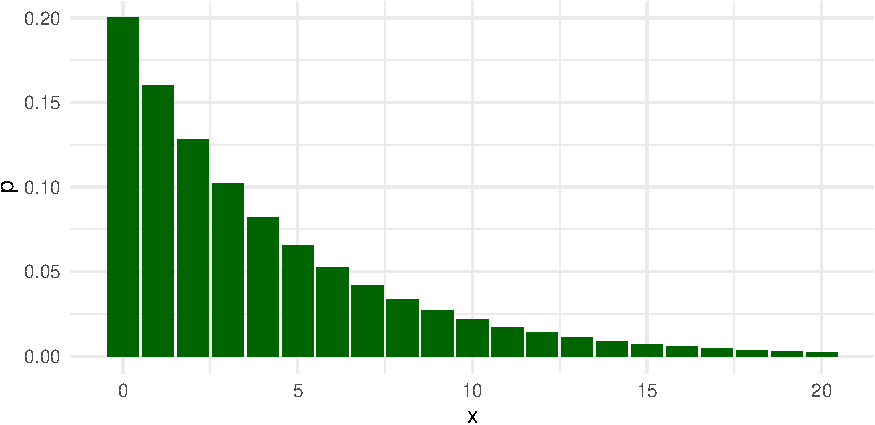
\includegraphics[width=0.75\linewidth]{Designing-Simulations-in-R_files/figure-latex/unnamed-chunk-28-1} \end{center}

The distribution is highly right-skewed, which suggests that the normal confidence interval might not work very well.

Now let's revise our previous simulation code to use the geometric distribution:

\begin{Shaded}
\begin{Highlighting}[]
\NormalTok{rps }\OtherTok{\textless{}{-}} \FunctionTok{replicate}\NormalTok{( }\DecValTok{1000}\NormalTok{, \{}
\NormalTok{  dat }\OtherTok{\textless{}{-}} \FunctionTok{rgeom}\NormalTok{( }\AttributeTok{n =} \DecValTok{10}\NormalTok{, }\AttributeTok{prob =} \DecValTok{1}\SpecialCharTok{/}\DecValTok{5}\NormalTok{)}
\NormalTok{  tt }\OtherTok{\textless{}{-}} \FunctionTok{t.test}\NormalTok{( dat )}
  \FunctionTok{findInterval}\NormalTok{( }\DecValTok{4}\NormalTok{, tt}\SpecialCharTok{$}\NormalTok{conf.int )}
\NormalTok{\})}
\FunctionTok{table}\NormalTok{( rps )}
\end{Highlighting}
\end{Shaded}

\begin{verbatim}
## rps
##   0   1   2 
##   8 892 100
\end{verbatim}

Our confidence interval is often entirely too low (such that the population mean is above the interval) and very rarely does our interval fall fully above the population mean.
Furthermore, our coverage rate is not 95\% as it should be:

\begin{Shaded}
\begin{Highlighting}[]
\FunctionTok{mean}\NormalTok{( rps }\SpecialCharTok{==} \DecValTok{1}\NormalTok{ )}
\end{Highlighting}
\end{Shaded}

\begin{verbatim}
## [1] 0.892
\end{verbatim}

To take account of Monte Carlo error, we will again do a proportion test.
The following test result calculates a confidence interval for the true coverage rate under the scenario we are examining:

\begin{Shaded}
\begin{Highlighting}[]
\NormalTok{covered }\OtherTok{\textless{}{-}} \FunctionTok{as.numeric}\NormalTok{( rps }\SpecialCharTok{==} \DecValTok{1}\NormalTok{ )}
\FunctionTok{prop.test}\NormalTok{( }\FunctionTok{sum}\NormalTok{(covered), }\FunctionTok{length}\NormalTok{(covered), }\AttributeTok{p =} \FloatTok{0.95}\NormalTok{)}
\end{Highlighting}
\end{Shaded}

\begin{verbatim}
## 
##  1-sample proportions test with continuity
##  correction
## 
## data:  sum(covered) out of length(covered), null probability 0.95
## X-squared = 69.605, df = 1, p-value <
## 2.2e-16
## alternative hypothesis: true p is not equal to 0.95
## 95 percent confidence interval:
##  0.8707042 0.9102180
## sample estimates:
##     p 
## 0.892
\end{verbatim}

Our coverage is \emph{too low}; the confidence interval based on the \(t\)-test misses the the true value more often than it should.

\section{Simulating across different scenarios}\label{simulating-across-different-scenarios}

So far, we have looked at coverage rates of the confidence interval under a single, specific scenario, with a sample size of 10, a population mean of 4, and a geometrically distributed variable.
We know from statistical theory (specifically, the central limit theorem) that the confidence interval should work better if the sample size is big enough.
But how big does it have to get?
One way to examine this question is to expand the simulation to look at several different scenarios involving different sample sizes.
We can think of this as a one-factor experiment, where we manipulate sample size and use simulation to estimate how confidence interval coverage rates change.

To implement such an experiment, we will write our own function that executes the full simulation process:

\begin{Shaded}
\begin{Highlighting}[]
\NormalTok{ttest\_CI\_experiment }\OtherTok{=} \ControlFlowTok{function}\NormalTok{( n ) \{}
  
\NormalTok{  rps }\OtherTok{\textless{}{-}} \FunctionTok{replicate}\NormalTok{( }\DecValTok{1000}\NormalTok{, \{}
\NormalTok{    dat }\OtherTok{\textless{}{-}} \FunctionTok{rgeom}\NormalTok{( }\AttributeTok{n =}\NormalTok{ n, }\AttributeTok{prob =} \DecValTok{1}\SpecialCharTok{/}\DecValTok{5}\NormalTok{) }\CommentTok{\# simulate data}
\NormalTok{    tt }\OtherTok{\textless{}{-}} \FunctionTok{t.test}\NormalTok{( dat )              }\CommentTok{\# analyze data}
    \FunctionTok{findInterval}\NormalTok{( }\DecValTok{4}\NormalTok{, tt}\SpecialCharTok{$}\NormalTok{conf.int )   }\CommentTok{\# evaluate coverage}
\NormalTok{  \})}

\NormalTok{  coverage }\OtherTok{\textless{}{-}} \FunctionTok{mean}\NormalTok{( rps }\SpecialCharTok{==} \DecValTok{1}\NormalTok{ )       }\CommentTok{\# summarize results}
  
  \FunctionTok{return}\NormalTok{(coverage)}
\NormalTok{\}}
\end{Highlighting}
\end{Shaded}

The code inside the body of the function is identical to what we've used above, but we've turned the sample size into a function argument, called \texttt{n}, because we want to be able to run the code for several different sample sizes.
With our function in hand, we can now run the simulation for a single scenario just by calling it:

\begin{Shaded}
\begin{Highlighting}[]
\FunctionTok{ttest\_CI\_experiment}\NormalTok{(}\AttributeTok{n =} \DecValTok{10}\NormalTok{)}
\end{Highlighting}
\end{Shaded}

\begin{verbatim}
## [1] 0.885
\end{verbatim}

Even though the sample size is still \texttt{n\ =\ 10}, the simulated coverage rate is a little bit different from what we found previously.
That's because there's some Monte Carlo error in each simulated coverage rate.

Our task is now to use this function for several different values of \(n\). We could just do this by copy-pasting and changing the value of \texttt{n}:

\begin{Shaded}
\begin{Highlighting}[]
\FunctionTok{ttest\_CI\_experiment}\NormalTok{(}\AttributeTok{n =} \DecValTok{10}\NormalTok{)}
\end{Highlighting}
\end{Shaded}

\begin{verbatim}
## [1] 0.922
\end{verbatim}

\begin{Shaded}
\begin{Highlighting}[]
\FunctionTok{ttest\_CI\_experiment}\NormalTok{(}\AttributeTok{n =} \DecValTok{20}\NormalTok{)}
\end{Highlighting}
\end{Shaded}

\begin{verbatim}
## [1] 0.91
\end{verbatim}

\begin{Shaded}
\begin{Highlighting}[]
\FunctionTok{ttest\_CI\_experiment}\NormalTok{(}\AttributeTok{n =} \DecValTok{30}\NormalTok{)}
\end{Highlighting}
\end{Shaded}

\begin{verbatim}
## [1] 0.914
\end{verbatim}

However, this will quickly get cumbersome if we want to evaluate many different sample sizes.
A better approach is to use a mapping function from the \texttt{purrr} package.\footnote{Alternately, readers familiar with the \texttt{*apply()} family of functions from Base R might prefer to use \texttt{lapply()} or \texttt{sapply()}, which do essentially the same thing as \texttt{purrr::map\_dbl()}.}
The \texttt{map\_dbl()} function takes a list of values and calls a function for each value in the list.\footnote{\href{https://r4ds.had.co.nz/iteration.html\#the-map-functions}{Section 21.5 of R for Data Science (1st edition)} provides an introduction to mapping.}
This accomplishes the same thing as using a \texttt{for} loop to iterate through a list of items, but is more succinct.
We'll first create a list of sample sizes to test out:

\begin{Shaded}
\begin{Highlighting}[]
\NormalTok{ns }\OtherTok{\textless{}{-}} \FunctionTok{c}\NormalTok{(}\DecValTok{10}\NormalTok{, }\DecValTok{20}\NormalTok{, }\DecValTok{30}\NormalTok{, }\DecValTok{40}\NormalTok{, }\DecValTok{60}\NormalTok{, }\DecValTok{80}\NormalTok{, }\DecValTok{100}\NormalTok{, }\DecValTok{120}\NormalTok{, }\DecValTok{140}\NormalTok{, }\DecValTok{160}\NormalTok{, }\DecValTok{180}\NormalTok{, }\DecValTok{200}\NormalTok{)}
\end{Highlighting}
\end{Shaded}

Now we can use \texttt{map\_dbl()} to evaluate the coverage rate for each sample size:

\begin{Shaded}
\begin{Highlighting}[]
\NormalTok{coverage\_est }\OtherTok{\textless{}{-}} \FunctionTok{map\_dbl}\NormalTok{( ns, ttest\_CI\_experiment)}
\end{Highlighting}
\end{Shaded}

It's helpful to depict simulation results graphically.
To do so, we will store the simulation results in a dataset and then create a line plot using a log scale for the horizontal axis:

\begin{Shaded}
\begin{Highlighting}[]
\NormalTok{res }\OtherTok{\textless{}{-}} \FunctionTok{data.frame}\NormalTok{( }
  \AttributeTok{n =}\NormalTok{ ns, }
  \AttributeTok{coverage =} \DecValTok{100} \SpecialCharTok{*}\NormalTok{ coverage\_est }
\NormalTok{)}

\FunctionTok{ggplot}\NormalTok{( res, }\FunctionTok{aes}\NormalTok{( }\AttributeTok{x =}\NormalTok{ n, }\AttributeTok{y =}\NormalTok{ coverage ) ) }\SpecialCharTok{+}
  \FunctionTok{geom\_hline}\NormalTok{( }\AttributeTok{yintercept=}\DecValTok{95}\NormalTok{, }\AttributeTok{col=}\StringTok{"red"}\NormalTok{ ) }\SpecialCharTok{+}   \CommentTok{\# reference line for nominal coverage rate}
  \FunctionTok{geom\_line}\NormalTok{() }\SpecialCharTok{+} 
  \FunctionTok{geom\_point}\NormalTok{( }\AttributeTok{size =} \DecValTok{4}\NormalTok{ ) }\SpecialCharTok{+}
  \FunctionTok{scale\_x\_log10}\NormalTok{( }\AttributeTok{breaks =}\NormalTok{ ns, }\AttributeTok{minor\_breaks =} \ConstantTok{NULL}\NormalTok{) }\SpecialCharTok{+}
  \FunctionTok{labs}\NormalTok{( }
    \AttributeTok{title=}\StringTok{"Coverage rates for t{-}test on exponential data"}\NormalTok{,}
    \AttributeTok{x =} \StringTok{"n (sample size)"}\NormalTok{, }
    \AttributeTok{y =} \StringTok{"coverage (\%)"} 
\NormalTok{  ) }\SpecialCharTok{+}
  \FunctionTok{coord\_cartesian}\NormalTok{(}\AttributeTok{xlim =} \FunctionTok{c}\NormalTok{(}\DecValTok{9}\NormalTok{,}\DecValTok{240}\NormalTok{), }\AttributeTok{ylim=}\FunctionTok{c}\NormalTok{(}\DecValTok{85}\NormalTok{,}\DecValTok{100}\NormalTok{), }\AttributeTok{expand =} \ConstantTok{FALSE}\NormalTok{) }\SpecialCharTok{+} 
  \FunctionTok{theme\_minimal}\NormalTok{()}
\end{Highlighting}
\end{Shaded}

\begin{center}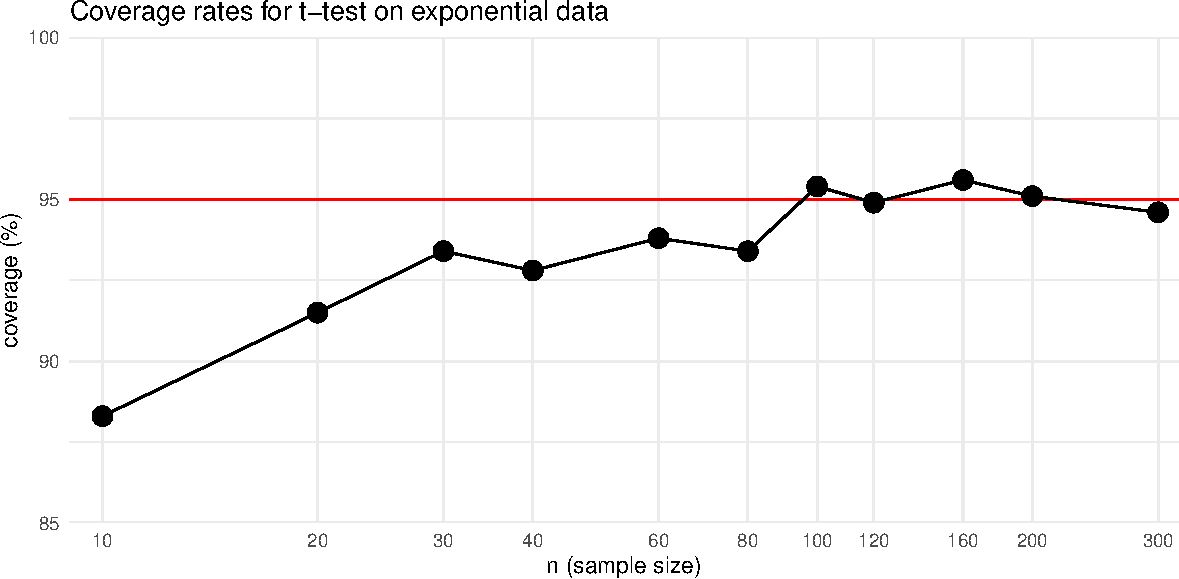
\includegraphics[width=0.75\linewidth]{Designing-Simulations-in-R_files/figure-latex/ttest_result_figure-1} \end{center}

We can see from the graph that the confidence interval's coverage rate improves as sample size gets larger. For sample sizes over 100, the interval appears to have coverage quite close to the nominal 95\% level.
Although the general trend is pretty clear, the graph is still a bit messy because each point is an \emph{estimated} coverage rate, with some Monte Carlo error baked in.

\section{Extending the simulation design}\label{extending-the-simulation-design}

So far, we have executed a simple simulation to assess how well a statistical method works in a given circumstance, then expanded the simulation by running a single-factor experiment in which we varied the sample size to see how the method's performance changes.
In our example, we found that coverage is below what it should be for small sample sizes, but improves for sample sizes in the 100's.

This example captures all the major steps of a simulation study, which we outlined at the start of Chapter \ref{introduction}.
We generated some hypothetical data according to a fully-specified data-generating process: either a normal distribution or a geometric distribution with a mean of 4.
We applied a defined data-analysis procedure to the simulated data: a confidence interval based on the \(t\) distribution.
We assessed how well the procedure worked across replications of the data-generating and data-analysis processes, in this case focusing on the coverage rate of the confidence interval.
After creating a function to implement this whole process for a single scenario, we investigated how the performance of the confidence interval changed depending on sample size.

In simulations of more complex models and data-analysis methods, some or all of the steps in the process might have more moving pieces or entail more complex calculations.
For instance, in the confidence interval simulation, we might want to compare the performance of several different approaches to calculating a confidence interval.
We might also want to examine how coverage rates are affected by other aspects of the data-generating process, such as looking at different population mean values for the geometric distribution---or even entirely different distributions.
With such additional layers of complexity, we will need to think systematically about each of the component parts of the simulation.
In the next chapter, we introduce an abstract, general framework for simulations that is helpful for guiding simulation design and managing all the considerations involved.

\section{Exercises}\label{exercises}

\begin{enumerate}
\def\labelenumi{\arabic{enumi}.}
\item
  The simulation function we developed in this chapter uses 1000 replications of the data-generating and data-analysis process, which leads to some Monte Carlo error in the simulation results. Modify the \texttt{ttest\_CI\_experiment()} function to make the number of replications an input argument, then re-run the simulation and re-create the graph of the results. What do your results indicate about when sample size is large enough to obtain nominal coverage?
\item
  Repeat the one-factor simulation, but using \(p = 1/10\) so that the population mean is \((1 - p) / p = 9\). How do the coverage rates change?
\item
  Modify the \texttt{ttest\_CI\_experiment()} function so that it returns a \texttt{data.frame} with the estimated coverage rate and the lower and upper end-points of a 95\% confidence interval for the true coverage rate (you can use \texttt{prop.test()} to obtain this). Re-run the simulations with the modified function and create a graph that depicts the coverage rates and the 95\% confidence intervals. (Hint: use the \texttt{ggplot2} function \texttt{geom\_pointrange()} to represent the confidence intervals.)
\end{enumerate}

\section{Challenges}\label{challenges}

\begin{enumerate}
\def\labelenumi{\arabic{enumi}.}
\setcounter{enumi}{3}
\item
  Here is a modified version of the \texttt{ttest\_CI\_experiment()} function that creates a data frame with lower and upper end-points of the simulated confidence intervals:

\begin{Shaded}
\begin{Highlighting}[]
\NormalTok{lotsa\_CIs\_experiment }\OtherTok{=} \ControlFlowTok{function}\NormalTok{( n ) \{}

\NormalTok{  lotsa\_CIs }\OtherTok{\textless{}{-}} \FunctionTok{replicate}\NormalTok{( }\DecValTok{1000}\NormalTok{, \{}
\NormalTok{    dat }\OtherTok{\textless{}{-}} \FunctionTok{rgeom}\NormalTok{( }\AttributeTok{n =}\NormalTok{ n, }\AttributeTok{prob =} \DecValTok{1}\SpecialCharTok{/}\DecValTok{5}\NormalTok{)                            }\CommentTok{\# simulate data}
\NormalTok{    tt }\OtherTok{\textless{}{-}} \FunctionTok{t.test}\NormalTok{( dat )                                         }\CommentTok{\# analyze data}
    \FunctionTok{data.frame}\NormalTok{(}\AttributeTok{lower =}\NormalTok{ tt}\SpecialCharTok{$}\NormalTok{conf.int[}\DecValTok{1}\NormalTok{], }\AttributeTok{upper =}\NormalTok{ tt.conf.int[}\DecValTok{2}\NormalTok{])  }\CommentTok{\# return CI}
\NormalTok{  \})}

  \CommentTok{\# summarize results}
  \CommentTok{\# \textless{}fill in the rest\textgreater{}}

  \FunctionTok{return}\NormalTok{(coverage)}
\NormalTok{\}}
\end{Highlighting}
\end{Shaded}

  Complete the function by writing code to compute the estimated coverage rate and a 95\% confidence interval for the true coverage rate.
\item
  Modify \texttt{ttest\_CI\_experiment()} or \texttt{lotsa\_CIs\_experiment()} so that the user can specify the population mean of the data-generating process. Also let the user specify the number of replications to use. Here is a function skeleton to use as a starting point:

\begin{Shaded}
\begin{Highlighting}[]
\NormalTok{ttest\_CI\_experiment }\OtherTok{\textless{}{-}} \ControlFlowTok{function}\NormalTok{( n, pop\_mean, reps) \{}

\NormalTok{  pop\_prob }\OtherTok{\textless{}{-}} \DecValTok{1} \SpecialCharTok{/}\NormalTok{ (pop\_mean }\SpecialCharTok{+} \DecValTok{1}\NormalTok{)}

  \CommentTok{\# \textless{}fill in the rest\textgreater{}}

  \FunctionTok{return}\NormalTok{(coverage)}
\NormalTok{\}}
\end{Highlighting}
\end{Shaded}
\item
  Using the modified function from the previous problem, implement a two-factor simulation study for several different values of \texttt{n} and several different population means.
\end{enumerate}

\part{Structure and Mechanics of a Simulation Study}\label{part-structure-and-mechanics-of-a-simulation-study}

\chapter{Structure of a simulation study}\label{structure-of-a-simulation-study}

Monte Carlo simulation is a very flexible tool that researchers apply to study a vast array of different models and topics.
However, within the realm of methodological studies, simulations share a common structure, nearly always involving the same set of steps or component pieces.
In learning to design your own simulations, it is very useful to recognize the core, abstract components that most simulation studies share.
Identifying these components will help you to organize your work and structure the coding tasks involved in writing a simulation.

In this chapter, we outline the component structure of a methodological simulation study, highlighting the four steps involved in a simulation of a single scenario and the three additional steps involved in multifactor simulations.
We then describe a strategy for implementing simulations that mirrors the same component structure, where each step in the simulation is represented by a separate function or object.
We call this strategy \textbf{\emph{tidy, modular simulation}}.
Finally, we show how the tidy, modular simulation strategy informs the structure and organization of code for a simulation study, walking through basic code skeletons (cf.~\ref{function-skeletons}) for each of the steps in a single-scenario simulation.

\section{General structure of a simulation}\label{general-structure-of-a-simulation}

In Chapter \ref{introduction} we described the four main steps involved in a simulation study. These steps are summarized in the top portion of Table \ref{tab:simulation}.

\begin{longtable}[]{@{}
  >{\raggedright\arraybackslash}p{(\columnwidth - 4\tabcolsep) * \real{0.0909}}
  >{\raggedright\arraybackslash}p{(\columnwidth - 4\tabcolsep) * \real{0.5152}}
  >{\raggedright\arraybackslash}p{(\columnwidth - 4\tabcolsep) * \real{0.3939}}@{}}
\caption{\label{tab:simulation} Steps in the Simulation Process}\tabularnewline
\toprule\noalign{}
\begin{minipage}[b]{\linewidth}\raggedright
\end{minipage} & \begin{minipage}[b]{\linewidth}\raggedright
Step
\end{minipage} & \begin{minipage}[b]{\linewidth}\raggedright
Description
\end{minipage} \\
\midrule\noalign{}
\endfirsthead
\toprule\noalign{}
\begin{minipage}[b]{\linewidth}\raggedright
\end{minipage} & \begin{minipage}[b]{\linewidth}\raggedright
Step
\end{minipage} & \begin{minipage}[b]{\linewidth}\raggedright
Description
\end{minipage} \\
\midrule\noalign{}
\endhead
\bottomrule\noalign{}
\endlastfoot
1 & \textbf{Generate} & Generate a sample of artificial data based on a specific statistical model or data-generating process. \\
2 & \textbf{Analyze} & Apply one or more data-analysis procedures, estimators, or workflows to the artificial data. \\
3 & \textbf{Repeat} & Repeat steps (1) \& (2) \(R\) times, recording \(R\) sets of results. \\
4 & \textbf{Summarize} & Assess the performance of the procedure across the \(R\) replications. \\
5 & \textbf{Design} & Specify a set of conditions to examine \\
6 & \textbf{Execute} & Run the simulation for each condition in the design. \\
7 & \textbf{Synthesize} & Specify a set of conditions to examine \\
\end{longtable}

In the simple example presented in Chapter \ref{t-test-simulation}, we put each of these steps into action with R code:

\begin{itemize}
\tightlist
\item
  We used the geometric distribution as a data-generating process;
\item
  We used the confidence interval from a one-sample \(t\)-test as the data-analysis procedure;
\item
  We repeatedly simulated the confidence intervals with R's \texttt{replicate()} function; and
\item
  We summarized the results by estimating the fraction of the intervals that covered the population mean.
\end{itemize}

We also saw that it was helpful to wrap all of these steps up into a single function, so that we could run the simulation across multiple sample sizes.

These four initial steps are common and shared across nearly all simulations.
In our first example, each of the steps was fairly simple, sometimes involving only a single line of code.
More generally, each of the steps might be quite a bit more complex. The data-generating process might involve a more complex model with multiple variables or multilevel structure.
The data analysis procedure might involve solving a multidimensional optimization problem to get parameter estimates, or might involve a data analysis workflow with multiple steps or contingencies.
Further, we might use more than one metric for summarizing the results across replications and describing the performance of the data analysis procedure.
Because each of the four steps involves its own set of choices, it will useful to recognize them as distinct from one another.

In methodological research projects, we usually want to examine simulation results across an array of different conditions that differ not only in terms of sample size, but also in other parameters or features of the data-generating process.
Running a simulation study across multiple conditions entails several further steps, which are summarized in the bottom portion of Table \ref{tab:simulation}. We will first need to specify the factors and specific conditions to be examined in our experimental design. We will then need to execute the simulation for each of the conditions and store all the results for further analysis. Finally, we will need to find ways to synthesize or make sense of the main patterns in the results across all of the conditions in the design.

Just as with the first four steps, it is useful to recognize these further steps as distinct from one another, each involving its own set of choices and techniques.
The design step requires choosing which parameters and features of the data-generating process to vary, as well as which specific values to use for each factor that is varied.
Executing a simulation might require a lot of computing power, especially if the simulation design has many conditions or the data analysis procedure takes a long time to compute.
How to effectively implement the execution step will therefore depend on the computing requirements and available resources.
Finally, many different techniques can be used to synthesizing findings from a multifactor simulation.
Which ones are most useful will depend on one's research questions and the choices made in each of the preceeding steps.
Across all seven steps, recognizing the distinct pieces will let us more effectively tackle the many decisions involved in designing and running a simulation.

\section{Tidy, modular simulations}\label{tidy-modular-simulations}

It is apparent from Table \ref{tab:simulation} that writing a simulation in R involves a bunch of considerations.
Considering the number of choices to be made, it is critical to stay organized and to approach the process systematically.
Recognizing the components of a simulation is the starting point.
Next is to see how to translate the components into R code.

n our own methodological work, we have found it very useful to always follow the same approach to writing code for a simulation.
We call this approach \emph{tidy, modular simulation}. It involves two simple principles:

\begin{enumerate}
\def\labelenumi{\arabic{enumi}.}
\tightlist
\item
  Implement each component of a simulation as its own, separate function or object.
\item
  Store all results in rectangular data sets.
\end{enumerate}

Writing separate functions for each component step of a simulation has several benefits.
The first is the practical benefit of turning the coding process from a monolithic (and potentially daunting) activity into a set of smaller, discrete tasks.
This lets us focus on one task at a time and makes it easier to see progress.
Second, following this principle makes for code that is easier to read, test, and debug.
Rather than having to scan through an entire code file to understand how the data analysis procedure is implemented, we can quickly identify the function that implements it, then focus on understanding the working of that function.
Likewise, if another researcher wanted to test out the data analysis procedure on a dataset of their own, they could do so by running the corresponding function rather than having to dissect an entire script.
Third, writing separate code for each component makes it possible to tweak the code or swap out pieces of the simulation, such as by adding additional estimation methods or trying out a data-generating process with different distributional assumptions.
We've already seen this in the example from Chapter \ref{t-test-simulation}, where we modified our initial data-generating process to use a geometric distribution rather than a normal distribution.
In short, following the first principle makes for simpler, more robust code that is easier to navigate and extend.

The second principle of tidy, modular simulation is to store all results in rectangular datasets, such as the base R \texttt{data.frame} object or the tidyverse \texttt{tibble} object.\footnote{\citet{Wickham2014tidydata} provides a broader introduction to the concept of tidy data in the context of data-analysis tasks.}
This principle applies to any and all output, including the simulated data from Step 1, the results of data analysis procedures from Step 2, full sets of replicated simulation results from Step 3, and summarized results from Step 4.
A primary benefit of following this principle is that it facilitates working with the output of each stage in the simulation process.
Analysts who are comfortable using R to analyze real data will find that they can use the same skills and tools to examine simulation output if it is in tabular form.
Many of the data processing and data analysis tools available in R work with---or even require---rectangular datasets.
Thus, using rectangular datasets makes it easier to inspect, summarize, and even visualize the output.

\section{Skeleton of a simulation study}\label{skeleton-of-a-simulation-study}

The principles of tidy simulation imply that code for a simulation study should usually follow the same broad outline and organization, involving functions for each step in process.
We will describe the outlines of simulation code using function skeletons to illustrate the inputs and outputs of each component.
These skeletons skip over all the specific details, so that we can see the structure more clearly.
We will first examine the structure of the code for simulating one specific scenario, then consider how to extend the code to systematically explore a variety of scenarios, as in a multifactor simulation.

First, let's look at the structure of the first four steps:

\begin{Shaded}
\begin{Highlighting}[]
\CommentTok{\# Generate (data{-}generating process)}

\NormalTok{generate\_data }\OtherTok{\textless{}{-}} \ControlFlowTok{function}\NormalTok{( model\_params ) \{}
  \CommentTok{\# stuff}
  \FunctionTok{return}\NormalTok{(data)}
\NormalTok{\}}

\CommentTok{\# Analyze (data{-}analysis procedure)}

\NormalTok{analyze }\OtherTok{\textless{}{-}} \ControlFlowTok{function}\NormalTok{( data ) \{}
  \CommentTok{\# stuff}
  \FunctionTok{return}\NormalTok{(one\_result)}
\NormalTok{\}}

\CommentTok{\# Repeat}

\NormalTok{one\_run }\OtherTok{\textless{}{-}} \ControlFlowTok{function}\NormalTok{( model\_params ) \{}
\NormalTok{  dat }\OtherTok{\textless{}{-}} \FunctionTok{generate\_data}\NormalTok{( model\_params )}
\NormalTok{  one\_result }\OtherTok{\textless{}{-}} \FunctionTok{analyze}\NormalTok{(dat)}
  \FunctionTok{return}\NormalTok{(one\_result)}
\NormalTok{\}}

\NormalTok{results }\OtherTok{\textless{}{-}} \FunctionTok{map\_df}\NormalTok{(}\DecValTok{1}\SpecialCharTok{:}\NormalTok{R, \textbackslash{}(x) }\FunctionTok{one\_run}\NormalTok{( params ))}

\CommentTok{\# Summarize (calculate performance measures)}

\NormalTok{assess\_performance }\OtherTok{\textless{}{-}} \ControlFlowTok{function}\NormalTok{( results, model\_params ) \{}
  \CommentTok{\# stuff}
  \FunctionTok{return}\NormalTok{(performance\_measures)}
\NormalTok{\}}

\FunctionTok{assess\_performance}\NormalTok{(results, params)}
\end{Highlighting}
\end{Shaded}

The code above shows the full skeleton of the simulation.
It involves four functions, where the outputs of one function get used as inputs in subsequent functions.
We will now look at the inputs and outputs of each function to see how they align with the four steps in the simulation process.
Subsequent chapters examine each piece in much greater detail---putting meat on the bones of each function skeleton, to torture our metafor---and discussing techniques and examples of how to design the components.

Besides illustrating the skeletal framework of a simulation, readers might find it useful to use it as a template from which to start writing their own code.
The \texttt{simhelpers} package includes the function \texttt{create\_skeleton()}, which will open a new R script that contains a template for a simulation study, with sections corresponding to each component:

\begin{Shaded}
\begin{Highlighting}[]
\NormalTok{simhelpers}\SpecialCharTok{::}\FunctionTok{create\_skeleton}\NormalTok{()}
\end{Highlighting}
\end{Shaded}

The template that appears is a slightly more elaborate version of the code above, with the main difference being that it also includes some additional lines of code to wire the pieces together for a multifactor simulation.
Starting from this template, you will already be well on the road to writing a tidy, modular simulation.

\subsection{Data-Generating Process}\label{data-generating-process}

The first step in a simulation is specifying a data-generating process. This is a hypothetical model for how data might arise, involving measurements or observations of one or more variables. The bare-bones skeleton of a data-generating function looks like the following:

\begin{Shaded}
\begin{Highlighting}[]
\NormalTok{generate\_data }\OtherTok{\textless{}{-}} \ControlFlowTok{function}\NormalTok{( model\_params ) \{}
  \CommentTok{\# stuff}
  \FunctionTok{return}\NormalTok{(data)}
\NormalTok{\}}
\end{Highlighting}
\end{Shaded}

The function takes as input a set of model parameter values, denoted here as \texttt{model\_params}.
Based on those model parameters, the function generates a hypothetical dataset as output.
Generating our own data based on a model allows us to know what the answer is (e.g., the true population mean or the true average effect of an intervention), so that we have benchmark against which to compare the results of a data analysis procedure that generates noisy estimates of the true value.

In practice, \texttt{model\_params} will usually not be just one input but rather a set of multiple input arguments.
The arguments might include inputs such as the population mean for a variable, the standard deviation of a distribution of treatment effects, or a parameter controlling the degree of skewness in the population distribution.
Many data-generating processes involving multiple variables, such as the response variable and predictor variables in a regression model.
In such instances, the inputs of \texttt{generate\_data()} might also include parameters that determine the degree of dependence or correlation between variables.
Further, the \texttt{generate\_data()} inputs will also usually include arguments relating to the sample size and structure of the hypothetical dataset.
For instance, in a simulation of a multilevel dataset where individuals are nested within clusters, the inputs might include an arguments to specify the total number of clusters and the average number of individuals per cluster.
We discuss the inputs and form of the data-generating function further in Chapter \ref{data-generating-processes}.

\subsection{Data Analysis Procedure}\label{data-analysis-procedure}

The second step in a simulation is specifying a data analysis procedure or set of procedures.
The bare-bones skeleton of a data-generating function looks like the following:

\begin{Shaded}
\begin{Highlighting}[]
\NormalTok{analyze }\OtherTok{\textless{}{-}} \ControlFlowTok{function}\NormalTok{( data ) \{}
  \CommentTok{\# stuff}
  \FunctionTok{return}\NormalTok{(one\_result)}
\NormalTok{\}}
\end{Highlighting}
\end{Shaded}

The function should take a single dataset as input and produce a set of estimates or results (e.g., point estimates, standard errors, confidence intervals, p-values, predictions, etc.).
Because we will be using the function to analyze hypothetical datasets simulated from the data-generating process, the \texttt{analyze()} function needs to work with \texttt{data} inputs that are produced by the \texttt{generate\_data()} function.
Thus, the code in the body of \texttt{analyze()} can assume that \texttt{data} will include relevant variables with specific names.

Inside the body of the function, \texttt{analyze()} includes code to carry out a data analysis procedure.
This might involve conducting a hypothesis test, as in the example from Chapter \ref{t-test-simulation}.
In another context, it might involve estimating an average growth rate from along with a standard error, given on a dataset with longitudinal repeated measurements from multiple individuals.
In still another context, it might involve generating individual-level predictions from a machine learning algorithm.
In simulations that involve comparing multiple analysis methods, we might write an \texttt{analyze()} function for each of the methods of interest, or we might write one function that does the calculations for all of the methods.

A well-written estimation method should, in principle, work not only on a simulated, hypothetical dataset but also on a real empirical dataset that has the same format (i.e., appropriate variable names and structure).
Because of this, the inputs of the \texttt{analyze()} function should not typically include any information about the parameters of the data-generating process.
To be realistic, the code for our simulated data-analysis procedure should not make use of anything that the analyst could not know when analyzing a real dataset.
Thus, \texttt{analyze()} has an argument for the sample dataset but not for \texttt{model\_params}.
We discuss the form and content of the data analysis function further in Chapter \ref{data-analysis-procedures}.

\subsection{Repetition}\label{repetition}

The third step in a simulation is to repeatedly evaluate the data-generating process and data analysis procedure.
In practice, this amounts to calling the \texttt{generate\_data()} function and then running the \texttt{analyze()} function on the result.
Here is the skeleton from our simulation template:

\begin{Shaded}
\begin{Highlighting}[]
\NormalTok{one\_run }\OtherTok{\textless{}{-}} \ControlFlowTok{function}\NormalTok{( model\_params ) \{}
\NormalTok{  dat }\OtherTok{\textless{}{-}} \FunctionTok{generate\_data}\NormalTok{( model\_params )}
\NormalTok{  one\_result }\OtherTok{\textless{}{-}} \FunctionTok{analyze}\NormalTok{(dat)}
  \FunctionTok{return}\NormalTok{(one\_result)}
\NormalTok{\}}

\NormalTok{results }\OtherTok{\textless{}{-}} \FunctionTok{map\_dfr}\NormalTok{(}\DecValTok{1}\SpecialCharTok{:}\NormalTok{R, \textbackslash{}(x) }\FunctionTok{one\_run}\NormalTok{( params ))}
\end{Highlighting}
\end{Shaded}

We first create a helper function called \texttt{one\_run()}, which takes \texttt{model\_params} as input.
Inside the body of the function, we call the \texttt{generate\_data()} function to simulate a hypothetical dataset.
We pass this dataset to \texttt{analyze()} and return a small dataset containing the results of the data-analysis procedure.
The \texttt{one\_run()} method is like a coordinator or dispatcher of the system: it generates the data, calls all the evaluation methods we want to call, combines all the results, and hands them back for recording.
Making a helper method such as \texttt{one\_run()} can be helpful because it facilitates debugging.

Once we have the \texttt{one\_run()} helper function, we need a way to call it repeatedly. As with many things in R, there are a variety of different ways to do something over and over.
In the above skeleton, we use the \texttt{map\_dfr()} function from the \texttt{purrr} package.\footnote{In the example from Chapter \ref{t-test-simulation}, we used the \texttt{replicate()} function from base R to repeat the process of generating and analyzing data.
  This function is a fine alternative to the \texttt{map\_dfr()} approach demonstrated in the skeleton.
  The only drawback is that it requires some further work to combine the results across replications.
  Here is a different version of the skeleton, which uses \texttt{replicate()} instead of \texttt{map\_dfr()}:

\begin{Shaded}
\begin{Highlighting}[]
\NormalTok{results\_list }\OtherTok{\textless{}{-}} \FunctionTok{replicate}\NormalTok{(}\AttributeTok{n =}\NormalTok{ R, }\AttributeTok{expr =}\NormalTok{ \{}
\NormalTok{  dat }\OtherTok{\textless{}{-}} \FunctionTok{generate\_data}\NormalTok{( params )}
\NormalTok{  one\_result }\OtherTok{\textless{}{-}} \FunctionTok{analyze}\NormalTok{(dat)}
  \FunctionTok{return}\NormalTok{(one\_result)}
\NormalTok{\}, }\AttributeTok{simplify =} \ConstantTok{FALSE}\NormalTok{)}

\NormalTok{results }\OtherTok{\textless{}{-}} \FunctionTok{list\_rbind}\NormalTok{(results\_list)}
\end{Highlighting}
\end{Shaded}

  This version of the skeleton does not create a \texttt{one\_run()} helper function, but instead puts the code from the body of \texttt{one\_run()} directly into the \texttt{expr} argument of \texttt{replicate()}.}
In the first argument, we specify a list of indices, one for each time we want to repeat the simulation process.
In the second argument, we specify a function that evaluates \texttt{one\_run()} for specified values of the model parameters stored in \texttt{params}.
The \texttt{map\_dfr()} function then calls the function on each entry in the list of indices, repeating the simulation process \texttt{R} times in all.
The function then stacks up all of the replications into a big dataset, with one or more rows per replication.\footnote{The \texttt{\_dfr} suffix in \texttt{map\_dfr()} stands for \texttt{data.frame} by row, meaning that each evaluation should produce a \texttt{data.frame} as output, and the outputs will be stacked by row.}

We go into further detail about how to approach running the simulation process in Chapter \ref{running-the-simulation-process}.
Among other things, we will illustrate how to use the \texttt{simhelpers} package to automate the process of coding this step, thereby avoiding the need to write a \texttt{one\_run()} helper function.

\subsection{Performance summaries}\label{performance-summaries}

The fourth step in a simulation is to summarize the distribution of simulation across replications.
Here is the skeleton from our simulation template:

\begin{Shaded}
\begin{Highlighting}[]
\NormalTok{assess\_performance }\OtherTok{\textless{}{-}} \ControlFlowTok{function}\NormalTok{( results, model\_params ) \{}
  \CommentTok{\# stuff}
  \FunctionTok{return}\NormalTok{(performance\_measures)}
\NormalTok{\}}

\FunctionTok{assess\_performance}\NormalTok{(results, params)}
\end{Highlighting}
\end{Shaded}

The \texttt{assess\_performance()} function takes \texttt{results} as input, which should be a dataset containing all of the replications of the data-generating and analysis process.
Its other input is \texttt{model\_params}, which includes the true parameter values of the data-generating process.
The function then uses these inputs to calculate performance measures and returns a summary of the performance measures in a dataset.

Performance measures are the metrics or criteria used to assess the performance of a statistical method across repeated samples from the data-generating process.
For example, we might want to know how close an estimator gets to the target parameter, on average, using a measure called root mean-squared error.
We might want to know if a confidence interval captures the truth parameter the right proportion of the time, as in the simulation from Chapter \ref{t-test-simulation}.
Performance measures are defined in terms of the sampling distribution of estimators or analysis results, across an infinite number of replications of the data-generating process.
In practice, we use many replications of the process, but still only a finite number. Consequently, we actually \emph{estimate} the performance measures and need to attend to the Monte Carlo error in the estimates.
We discuss the specifics of different performance measures and assessment of Monte Carlo error in Chapter \ref{performance-criteria}.

\subsection{Multifactor simulations}\label{multifactor-simulations}

Thus far, we have sketched out the structure of a modular, tidy simulation for a single context.
In our \(t\)-test case study, for example, we might ask how well the \(t\)-test works when we have \(n=100\) units and the observations follow geometric distribution.
However, we rarely want to examine a method only in a single context.
Typically, in we will want to explore how well a procedure works across a range of different contexts.
If we choose conditions in a structured and thoughtful manner, we will be able to examine broad trends and potentially make more general claims about the behaviors of the data-analysis procedures under investigation.
Thus, it is helpful to think of simulations as akin to a designed experiment: in seeking to understand the properties of one or more procedures, we test them under a variety of different scenarios to see how they perform, then seek to identify more general patterns that hold beyond the specific scenarios examined.
This is the heart of simulation for methodological evaluation.

To implement a multifactor simulation, we will follows the same principles of modular, tidy simulation.
In particular, we will take the code developed for simulating a single context and combine it into a function that can be evaluated for any and all scenarios of interest.
Simulation studies often follow a full factorial design, in which each level of a factor (something we vary, such as sample size, true treatment effect, or residual variance) is crossed with every other level.
The experimental design then consists of sets of parameter values (including design parameters, such as sample sizes), and these too can be represented in an object, distinct from the other components of the simulation.
We will discuss multiple-scenario simulations in Part III (starting with Chapter \ref{exp-design}, after we more fully develop the core concepts and techniques involved in simulating a single context.

\chapter{Case Study: Heteroskedastic ANOVA}\label{case-ANOVA}

In this chapter, we present another detailed example of a simulation study, which demonstrates how to put the tidy, modular simulation strategy into practice.

To illustrate the process of programming a simulation, we reconstruct the simulations from Brown and Forsythe (1974).
We also use this case study as a recurring example in some of the following chapters.

Brown and Forsythe wanted to study methods for null hypothesis testing in the following model: Consider a population consisting of \(g\) separate groups, with population means \(\mu_1,...,\mu_g\) and population variances \(\sigma_1^2,...,\sigma_g^2\) for some characteristic \(X\).
We obtain samples of size \(n_1,...,n_g\) from each of the groups, and take measurements of the characteristic for each sampled unit.
Let \(x_{ij}\) denote the measurement from unit \(i\) in group \(j\), for \(i = 1,...,n_j\) for each \(j = 1,..., g\).
Our goal is to use the sample data to test the hypothesis that the population means are all equal, i.e.,
\[
H_0: \mu_1 = \mu_2 = \cdots = \mu_g.
\]
Now, if the population \emph{variances} were all equal (i.e., \(\sigma_1^2 = \sigma_2^2 = \cdots = \sigma_g^2\)), we could use a conventional one-way analysis of variance (ANOVA) to test.
However, one-way ANOVA might not work well if the variances are not equal.
The question is then what are best practices for testing, when in this heteroskedastic case.

To tackle this question, Brown and Forsythe evaluated two different hypothesis testing procedures, developed by James (1951) and Welch (1951), that had been proposed for testing this hypothesis without assuming equality of variances, along with the conventional one-way ANOVA F-test as a benchmark.
They also proposed and evaluated a new procedure of their own devising.
(This latter pieces makes this paper one of a canonical format for statistical methodology papers: find some problem that current procedures do not perfectly solve, invent something to do a better job, and then do simulation and/or math to build a case that the new procedure is better.)
Overall, the simulation involves comparing the performance of these different hypothesis testing procedures (the methods) under a range of conditions (different data generating processes).

For hypothesis testing, there are two main performance metrics of interest: type-I error rate and power.
The type-I error rate is, when the null hypothesis is true, how often a test falsely rejects the null.
It is a measure of how \emph{valid} a method is.
Power is how often a test correctly rejects the null when it is indeed false.
It is a measure of how \emph{powerful} (or sensitive) a method is.
The authors explored error rates and power for nominal \(\alpha\)-levels of 1\%, 5\%, and 10\%.
Table 1 of their paper reports the simulation results for type-I error (labeled as ``size''); ideally, a test should have true type-I error very close to the nominal \(\alpha\).

They looked at ten different scenarios:

\begin{table}

\caption{\label{tab:BF-scenarios}Scenarios explored by Brown and Forsythe from their Table 1}
\centering
\begin{tabular}[t]{l|l|l}
\hline
Groups & Sample Sizes & Standard Deviations\\
\hline
4 & 4,4,4,4 & 1,1,1,1\\
\hline
4 & 4,8,10,12 & 1,2,2,3\\
\hline
4 & 11,11,11,11 & 1,1,1,1\\
\hline
4 & 11,16,16,21 & 1,2,2,3\\
\hline
6 & 4,4,4,4,4,4 & 1,1,1,1,1,1\\
\hline
6 & 4,6,6,8,10,12 & 1,2,2,3\\
\hline
6 & 6,6,6,6,6,6 & 1,1,1,1,1,1\\
\hline
6 & 11,11,11,11,11,11 & 1,1,1,1,1,1\\
\hline
6 & 16,16,16,16,16,16 & 1,2,2,3\\
\hline
6 & 21,21,21,21,21,21 & 1,2,2,3\\
\hline
10 & 20,20,20,20,20,20,20,20,20,20 & 1,1,1.5,1.5,2,2,2.5,2.5,3,3\\
\hline
\end{tabular}
\end{table}

We also provide some of the numbers they reported in their Table 1 for these scenarios on Table \ref{tab:BF-table1}.

\begin{table}

\caption{\label{tab:BF-table1}Portion of "Table 1," reproduced from Brown and Forsythe}
\centering
\begin{tabular}[t]{r|r|r|r|r|r|r|r|r|r}
\hline
group & F\_10\% & F\_5\% & F\_1\% & F*\_10\% & F*\_5\% & F*\_1\% & W\_10\% & W\_5\% & W\_1\%\\
\hline
1 & 10.2 & 4.9 & 0.9 & 7.8 & 3.4 & 0.5 & 9.6 & 4.5 & 0.8\\
\hline
2 & 12.0 & 6.7 & 1.7 & 8.9 & 4.1 & 0.7 & 10.3 & 4.7 & 0.8\\
\hline
3 & 9.9 & 5.1 & 1.1 & 9.5 & 4.8 & 1.0 & 10.8 & 5.7 & 1.6\\
\hline
4 & 5.9 & 3.0 & 0.6 & 10.3 & 5.7 & 1.4 & 9.8 & 4.9 & 0.9\\
\hline
5 & 21.9 & 14.4 & 5.6 & 11.0 & 6.2 & 1.8 & 11.3 & 6.5 & 2.0\\
\hline
6 & 10.1 & 5.1 & 1.0 & 9.8 & 5.7 & 1.5 & 10.0 & 5.0 & 0.9\\
\hline
7 & 11.4 & 6.3 & 1.8 & 10.7 & 5.7 & 1.5 & 10.1 & 5.0 & 1.1\\
\hline
8 & 10.3 & 4.9 & 1.1 & 10.3 & 5.1 & 1.0 & 10.2 & 5.0 & 1.0\\
\hline
9 & 17.3 & 10.8 & 3.9 & 11.1 & 6.2 & 1.8 & 10.5 & 5.5 & 1.2\\
\hline
10 & 7.3 & 4.0 & 1.0 & 11.5 & 6.5 & 1.8 & 10.6 & 5.4 & 1.1\\
\hline
11 & 9.6 & 4.9 & 1.0 & 7.3 & 3.4 & 0.4 & 11.4 & 6.1 & 1.4\\
\hline
\end{tabular}
\end{table}

Table \ref{tab:BF-table1} reports results on power; it is desirable to have higher power to reject null hypotheses that are false, so higher rates are better here.

To replicate this simulation we are going to first write code to evaluate our three procedures in a specific scenario with a specific set of core parameters (e.g., sample sizes, number of groups, and so forth), and then scale up to do a range of scenarios where we vary these parameters.

\section{The data-generating model}\label{the-data-generating-model}

In the heteroskedastic one-way ANOVA simulation, there are three sets of parameter values: population means, population variances, and sample sizes.
Rather than attempting to write a general data-generating function immediately, it is often easier to write code for a specific case first and then use that code as a launch point for the rest.
For example, say that we have four groups with means of 1, 2, 5, 6; variances of 3, 2, 5, 1; and sample sizes of 3, 6, 2, 4:

\begin{Shaded}
\begin{Highlighting}[]
\NormalTok{mu }\OtherTok{\textless{}{-}} \FunctionTok{c}\NormalTok{(}\DecValTok{1}\NormalTok{, }\DecValTok{2}\NormalTok{, }\DecValTok{5}\NormalTok{, }\DecValTok{6}\NormalTok{)}
\NormalTok{sigma\_sq }\OtherTok{\textless{}{-}} \FunctionTok{c}\NormalTok{(}\DecValTok{3}\NormalTok{, }\DecValTok{2}\NormalTok{, }\DecValTok{5}\NormalTok{, }\DecValTok{1}\NormalTok{)}
\NormalTok{sample\_size }\OtherTok{\textless{}{-}} \FunctionTok{c}\NormalTok{(}\DecValTok{3}\NormalTok{, }\DecValTok{6}\NormalTok{, }\DecValTok{2}\NormalTok{, }\DecValTok{4}\NormalTok{)}
\end{Highlighting}
\end{Shaded}

Following Brown and Forsythe, we'll assume that the measurements are normally distributed within each sub-group of the population. The following code generates a vector of group id's and a vector of simulated measurements:

\begin{Shaded}
\begin{Highlighting}[]
\NormalTok{N }\OtherTok{\textless{}{-}} \FunctionTok{sum}\NormalTok{(sample\_size) }\CommentTok{\# total sample size}
\NormalTok{g }\OtherTok{\textless{}{-}} \FunctionTok{length}\NormalTok{(sample\_size) }\CommentTok{\# number of groups}

\CommentTok{\# group id}
\NormalTok{group }\OtherTok{\textless{}{-}} \FunctionTok{rep}\NormalTok{(}\DecValTok{1}\SpecialCharTok{:}\NormalTok{g, }\AttributeTok{times =}\NormalTok{ sample\_size)}

\CommentTok{\# mean for each unit of the sample}
\NormalTok{mu\_long }\OtherTok{\textless{}{-}} \FunctionTok{rep}\NormalTok{(mu, }\AttributeTok{times =}\NormalTok{ sample\_size) }

\CommentTok{\# sd for each unit of the sample}
\NormalTok{sigma\_long }\OtherTok{\textless{}{-}} \FunctionTok{rep}\NormalTok{(}\FunctionTok{sqrt}\NormalTok{(sigma\_sq), }\AttributeTok{times =}\NormalTok{ sample\_size) }

\CommentTok{\# See what we have?}
\FunctionTok{tibble}\NormalTok{( }\AttributeTok{group=}\NormalTok{group, }\AttributeTok{mu=}\NormalTok{mu\_long, }\AttributeTok{sigma=}\NormalTok{sigma\_long)}
\end{Highlighting}
\end{Shaded}

\begin{verbatim}
## # A tibble: 15 x 3
##    group    mu sigma
##    <int> <dbl> <dbl>
##  1     1     1  1.73
##  2     1     1  1.73
##  3     1     1  1.73
##  4     2     2  1.41
##  5     2     2  1.41
##  6     2     2  1.41
##  7     2     2  1.41
##  8     2     2  1.41
##  9     2     2  1.41
## 10     3     5  2.24
## 11     3     5  2.24
## 12     4     6  1   
## 13     4     6  1   
## 14     4     6  1   
## 15     4     6  1
\end{verbatim}

\begin{Shaded}
\begin{Highlighting}[]
\CommentTok{\# Now make our data}
\NormalTok{x }\OtherTok{\textless{}{-}} \FunctionTok{rnorm}\NormalTok{(N, }\AttributeTok{mean =}\NormalTok{ mu\_long, }\AttributeTok{sd =}\NormalTok{ sigma\_long)}
\FunctionTok{tibble}\NormalTok{(}\AttributeTok{group =}\NormalTok{ group, }\AttributeTok{x =}\NormalTok{ x)}
\end{Highlighting}
\end{Shaded}

\begin{verbatim}
## # A tibble: 15 x 2
##    group      x
##    <int>  <dbl>
##  1     1  0.130
##  2     1  4.22 
##  3     1 -0.504
##  4     2  1.70 
##  5     2 -0.112
##  6     2  1.27 
##  7     2  1.05 
##  8     2  2.92 
##  9     2  2.14 
## 10     3  2.88 
## 11     3  6.22 
## 12     4  4.53 
## 13     4  5.98 
## 14     4  6.55 
## 15     4  6.67
\end{verbatim}

We have made a small dataset of group membership and outcome.
We note that there are many different and legitimate ways of doing this in R.
E.g., we could generate each group separately, and then stack our groups, instead of using \texttt{rep} to do it all at once.
In general, we advocate the adage that if you can do it at all, then you should feel good about yourself.
Do not worry about writing code the ``best'' way when you are initially putting a simulation together.

To continue, as we are going to generate data over and over, we wrap this code in a function.
We also make our means, variances and sample sizes be parameters of our function so we can make datasets of different sizes and shapes, like so:

\begin{Shaded}
\begin{Highlighting}[]
\NormalTok{generate\_data }\OtherTok{\textless{}{-}} \ControlFlowTok{function}\NormalTok{(mu, sigma\_sq, sample\_size) \{}

\NormalTok{  N }\OtherTok{\textless{}{-}} \FunctionTok{sum}\NormalTok{(sample\_size)}
\NormalTok{  g }\OtherTok{\textless{}{-}} \FunctionTok{length}\NormalTok{(sample\_size)}

\NormalTok{  group }\OtherTok{\textless{}{-}} \FunctionTok{rep}\NormalTok{(}\DecValTok{1}\SpecialCharTok{:}\NormalTok{g, }\AttributeTok{times =}\NormalTok{ sample\_size)}
\NormalTok{  mu\_long }\OtherTok{\textless{}{-}} \FunctionTok{rep}\NormalTok{(mu, }\AttributeTok{times =}\NormalTok{ sample\_size)}
\NormalTok{  sigma\_long }\OtherTok{\textless{}{-}} \FunctionTok{rep}\NormalTok{(}\FunctionTok{sqrt}\NormalTok{(sigma\_sq), }\AttributeTok{times =}\NormalTok{ sample\_size)}

\NormalTok{  x }\OtherTok{\textless{}{-}} \FunctionTok{rnorm}\NormalTok{(N, }\AttributeTok{mean =}\NormalTok{ mu\_long, }\AttributeTok{sd =}\NormalTok{ sigma\_long)}
\NormalTok{  sim\_data }\OtherTok{\textless{}{-}} \FunctionTok{tibble}\NormalTok{(}\AttributeTok{group =}\NormalTok{ group, }\AttributeTok{x =}\NormalTok{ x)}

  \FunctionTok{return}\NormalTok{(sim\_data)}
\NormalTok{\}}
\end{Highlighting}
\end{Shaded}

The above code is simply the code we built previously, all bundled up.
Our workflow is to scrabble around to get it to work once, the way we want, and then bundle up our final work into a function for later reuse.

Given our method, we can easily call our function to get a new set of simulated data.
For example, to generate a dataset with the same parameters as before, we can do:

\begin{Shaded}
\begin{Highlighting}[]
\NormalTok{sim\_data }\OtherTok{\textless{}{-}} \FunctionTok{generate\_data}\NormalTok{(}\AttributeTok{mu =}\NormalTok{ mu, }\AttributeTok{sigma\_sq =}\NormalTok{ sigma\_sq, }
                          \AttributeTok{sample\_size =}\NormalTok{ sample\_size)}
\end{Highlighting}
\end{Shaded}

To generate one with 0s for the averages of each group, but the same group variances and sample sizes as before, we can do:

\begin{Shaded}
\begin{Highlighting}[]
\NormalTok{sim\_data\_null }\OtherTok{\textless{}{-}} \FunctionTok{generate\_data}\NormalTok{( }\AttributeTok{mu =} \FunctionTok{c}\NormalTok{( }\DecValTok{0}\NormalTok{, }\DecValTok{0}\NormalTok{, }\DecValTok{0}\NormalTok{, }\DecValTok{0}\NormalTok{ ),}
                                \AttributeTok{sigma\_sq =}\NormalTok{ sigma\_sq, }
                                \AttributeTok{sample\_size =}\NormalTok{ sample\_size)}
\end{Highlighting}
\end{Shaded}

\subsection{Coding remark}\label{coding-remark}

In the above, we built some sample code, and then bundled it into a function by literally cutting and pasting the initial work we did into a function skeleton.
In the process, we shifted from having variables in our workspace with different names to using those variable names as parameters in our function call.

Developing code in this way is not without hazards.
In particular, after finishing making our function, our workspace has a variable \texttt{mu} in it and our function also has a parameter named \texttt{mu}.
Inside the function, R will use the parameter \texttt{mu} first, but this is potentially confusing.
As are, potentially, lines such as \texttt{mu\ =\ mu}, which means ``set the function's parameter called \texttt{mu} to the variable called \texttt{mu}.''
These are different things (with the same name).

One way to check your code, once a function is built, is to comment out the initial code (or delete it), restart R or at least clear out the workspace, and then re-run the code that uses the function.
If things still work, then you should be somewhat confident you successfully bundled your code into the function.

You can also, once you bundle your code, do a search and replace to change variable names in your function to something more generic, to make the separation more clear.

\section{The estimation procedures}\label{the-estimation-procedures}

Brown and Forsythe considered four different hypothesis testing procedures for heteroskedastic ANOVA.
We start with the simplest one, which is just to use a conventional one-way ANOVA (while mistakenly assuming homoskedasticity). R's \texttt{oneway.test} function will actually calculate this test automatically:

\begin{Shaded}
\begin{Highlighting}[]
\NormalTok{sim\_data }\OtherTok{\textless{}{-}} \FunctionTok{generate\_data}\NormalTok{(}\AttributeTok{mu =}\NormalTok{ mu, }\AttributeTok{sigma\_sq =}\NormalTok{ sigma\_sq,}
                          \AttributeTok{sample\_size =}\NormalTok{ sample\_size)}
\FunctionTok{oneway.test}\NormalTok{(x }\SpecialCharTok{\textasciitilde{}} \FunctionTok{factor}\NormalTok{(group), }\AttributeTok{data =}\NormalTok{ sim\_data, }\AttributeTok{var.equal =} \ConstantTok{TRUE}\NormalTok{)}
\end{Highlighting}
\end{Shaded}

\begin{verbatim}
## 
##  One-way analysis of means
## 
## data:  x and factor(group)
## F = 11.481, num df = 3, denom df = 11,
## p-value = 0.001029
\end{verbatim}

The main result we need here is the \(p\)-value, which will let us assess the test's Type-I error and power for a given nominal \(\alpha\)-level. The following function takes simulated data as input and returns as output the \(p\)-value from a one-way ANOVA:

\begin{Shaded}
\begin{Highlighting}[]
\NormalTok{ANOVA\_F\_aov }\OtherTok{\textless{}{-}} \ControlFlowTok{function}\NormalTok{(sim\_data) \{}
\NormalTok{  oneway\_anova }\OtherTok{\textless{}{-}} \FunctionTok{oneway.test}\NormalTok{(x }\SpecialCharTok{\textasciitilde{}} \FunctionTok{factor}\NormalTok{(group), }\AttributeTok{data =}\NormalTok{ sim\_data,}
                              \AttributeTok{var.equal =} \ConstantTok{TRUE}\NormalTok{)}
  \FunctionTok{return}\NormalTok{(oneway\_anova}\SpecialCharTok{$}\NormalTok{p.value)}
\NormalTok{\}}

\FunctionTok{ANOVA\_F\_aov}\NormalTok{(sim\_data)}
\end{Highlighting}
\end{Shaded}

\begin{verbatim}
## [1] 0.001028701
\end{verbatim}

We might instead write the code to implement the ANOVA test ourselves.
This has some plusses (e.g., \texttt{oneway.test} maybe is doing a lot of other stuff which could take time and slow down our simulation) and minuses (e..g, writing our own code takes \emph{our} time, and it gives us lots of room to make mistakes and thus make life hard on ourself).
For further discussion of the trade-offs, see Chapter \ref{optimize-code}, where we do implement it by hand and see what kind of speed-ups we can obtain by doing that.

We next implement the Welch test, another one of the tests considered by Brown and Forsythe.
Here is a function that calculates the Welch test by hand, again following the notation and formulas from the paper:

\begin{Shaded}
\begin{Highlighting}[]
\NormalTok{Welch\_F }\OtherTok{\textless{}{-}} \ControlFlowTok{function}\NormalTok{(sim\_data) \{}

\NormalTok{  stats }\OtherTok{\textless{}{-}}\NormalTok{ sim\_data }\SpecialCharTok{\%\textgreater{}\%} \FunctionTok{group\_by}\NormalTok{( group ) }\SpecialCharTok{\%\textgreater{}\%}
    \FunctionTok{summarise}\NormalTok{( }\AttributeTok{x\_bar =} \FunctionTok{mean}\NormalTok{( x ),}
               \AttributeTok{s\_sq =} \FunctionTok{var}\NormalTok{( x ),}
               \AttributeTok{n =} \FunctionTok{n}\NormalTok{() )}
  
\NormalTok{  g }\OtherTok{=} \FunctionTok{nrow}\NormalTok{( stats )}

\NormalTok{  stats }\OtherTok{\textless{}{-}} \FunctionTok{mutate}\NormalTok{( stats, }
                   \AttributeTok{w =}\NormalTok{ n }\SpecialCharTok{/}\NormalTok{ s\_sq )}
  
\NormalTok{  res }\OtherTok{\textless{}{-}}\NormalTok{ stats }\SpecialCharTok{\%\textgreater{}\%}
    \FunctionTok{summarise}\NormalTok{( }\AttributeTok{u =} \FunctionTok{sum}\NormalTok{(w),}
               \AttributeTok{x\_tilde =} \FunctionTok{sum}\NormalTok{( w }\SpecialCharTok{*}\NormalTok{ x\_bar ) }\SpecialCharTok{/}\NormalTok{ u,}
               \AttributeTok{msbtw =} \FunctionTok{sum}\NormalTok{( w }\SpecialCharTok{*}\NormalTok{ (x\_bar }\SpecialCharTok{{-}}\NormalTok{ x\_tilde)}\SpecialCharTok{\^{}}\DecValTok{2}\NormalTok{ ) }\SpecialCharTok{/}\NormalTok{ (g }\SpecialCharTok{{-}} \DecValTok{1}\NormalTok{),}
               \AttributeTok{G =} \FunctionTok{sum}\NormalTok{( (}\DecValTok{1} \SpecialCharTok{{-}}\NormalTok{ w }\SpecialCharTok{/}\NormalTok{ u)}\SpecialCharTok{\^{}}\DecValTok{2} \SpecialCharTok{/}\NormalTok{ (n }\SpecialCharTok{{-}} \DecValTok{1}\NormalTok{) ),}
               \AttributeTok{denom =} \DecValTok{1} \SpecialCharTok{+}\NormalTok{  G }\SpecialCharTok{*} \DecValTok{2} \SpecialCharTok{*}\NormalTok{ (g }\SpecialCharTok{{-}} \DecValTok{2}\NormalTok{) }\SpecialCharTok{/}\NormalTok{ (g}\SpecialCharTok{\^{}}\DecValTok{2} \SpecialCharTok{{-}} \DecValTok{1}\NormalTok{),}
               \AttributeTok{W =}\NormalTok{ msbtw }\SpecialCharTok{/}\NormalTok{ denom,}
               \AttributeTok{f =}\NormalTok{ (g}\SpecialCharTok{\^{}}\DecValTok{2} \SpecialCharTok{{-}} \DecValTok{1}\NormalTok{) }\SpecialCharTok{/}\NormalTok{ (}\DecValTok{3} \SpecialCharTok{*}\NormalTok{ G) )}

\NormalTok{  pval }\OtherTok{\textless{}{-}} \FunctionTok{pf}\NormalTok{(res}\SpecialCharTok{$}\NormalTok{W, }\AttributeTok{df1 =}\NormalTok{ g }\SpecialCharTok{{-}} \DecValTok{1}\NormalTok{, }\AttributeTok{df2 =}\NormalTok{ res}\SpecialCharTok{$}\NormalTok{f, }\AttributeTok{lower.tail =} \ConstantTok{FALSE}\NormalTok{)}

  \FunctionTok{return}\NormalTok{(pval)}
\NormalTok{\}}

\FunctionTok{Welch\_F}\NormalTok{(sim\_data)}
\end{Highlighting}
\end{Shaded}

\begin{verbatim}
## [1] 0.02256937
\end{verbatim}

Our estimation function does not care if the data are simulated or not--we call the parameter \texttt{data} not \texttt{sim\_data} to reflect this.
Eventually, we might imagine using this function on our real data!
Also, we can put a lot of complex stuff in a function--and then forget all about it.
In the above, for example, you can understand everything we say about writing simulations even if you do not understand anything at all about what this function is doing: it is just a black box that takes data and returns a \(p\)-value.

\section{Running the simulation}\label{running-the-simulation}

We now have functions that implement steps 2 and 3 of the simulation.
Given some parameters, \texttt{generate\_data} produces a simulated dataset and \texttt{ANOVA\_F\_aov} and \texttt{Welch\_F} use the simulated data to calculate \(p\)-values two different ways.
We now want to know which way is better, and how.
To answer this question, we next need to repeat this chain of calculations a bunch of times.

We first make a function that puts our chain together in a single method.
This method is also responsible for putting the results together in a tidy structure that is easy to aggregate and analyze.

\begin{Shaded}
\begin{Highlighting}[]
\NormalTok{one\_run }\OtherTok{=} \ControlFlowTok{function}\NormalTok{( mu, sigma\_sq, sample\_size ) \{}
\NormalTok{  sim\_data }\OtherTok{\textless{}{-}} \FunctionTok{generate\_data}\NormalTok{(}\AttributeTok{mu =}\NormalTok{ mu, }\AttributeTok{sigma\_sq =}\NormalTok{ sigma\_sq,}
                            \AttributeTok{sample\_size =}\NormalTok{ sample\_size)}
\NormalTok{  anova\_p }\OtherTok{\textless{}{-}} \FunctionTok{ANOVA\_F\_aov}\NormalTok{(sim\_data)}
\NormalTok{  Welch\_p }\OtherTok{\textless{}{-}} \FunctionTok{Welch\_F}\NormalTok{(sim\_data)}
  \FunctionTok{tibble}\NormalTok{(}\AttributeTok{ANOVA =}\NormalTok{ anova\_p, }\AttributeTok{Welch =}\NormalTok{ Welch\_p)}
\NormalTok{\}}

\FunctionTok{one\_run}\NormalTok{( }\AttributeTok{mu =}\NormalTok{ mu, }\AttributeTok{sigma\_sq =}\NormalTok{ sigma\_sq, }\AttributeTok{sample\_size =}\NormalTok{ sample\_size )}
\end{Highlighting}
\end{Shaded}

\begin{verbatim}
## # A tibble: 1 x 2
##       ANOVA    Welch
##       <dbl>    <dbl>
## 1 0.0000530 0.000568
\end{verbatim}

A single simulation trial simply does steps 2 and 3, ending with a nice dataframe or tibble that has our results for that single run.

We next call \texttt{one\_run()} over and over; see \ref{repeating-oneself} for some discussion of options.
The following uses \texttt{map\_df} to run \texttt{one\_run()} 4 times and then stack the results into a single data frame (the \texttt{\_df} tells R to do the stacking):

\begin{Shaded}
\begin{Highlighting}[]
\NormalTok{sim\_data }\OtherTok{\textless{}{-}} \FunctionTok{map\_df}\NormalTok{(}\DecValTok{1}\SpecialCharTok{:}\DecValTok{4}\NormalTok{,}
                  \SpecialCharTok{\textasciitilde{}} \FunctionTok{one\_run}\NormalTok{(}\AttributeTok{mu =}\NormalTok{ mu, }\AttributeTok{sigma\_sq =}\NormalTok{ sigma\_sq,}
                          \AttributeTok{sample\_size =}\NormalTok{ sample\_size) )}
\NormalTok{sim\_data}
\end{Highlighting}
\end{Shaded}

\begin{verbatim}
## # A tibble: 4 x 2
##        ANOVA    Welch
##        <dbl>    <dbl>
## 1 0.00141    0.0321  
## 2 0.00143    0.0587  
## 3 0.00000282 0.000567
## 4 0.00924    0.0855
\end{verbatim}

Voila! We have simulated \(p\)-values!

\section{Analyzing the Simulation}\label{analyzing-the-simulation}

We now have all the pieces in place to reproduce the results from Brown and Forsythe (1974).
We first focus on calculating the actual type-I error rate of these tests---that is, the proportion of the time that they reject the null hypothesis of equal means when that null is actually true---for an \(\alpha\)-level of .05.
We therefore need to simulate data according to process where the population means are indeed all equal. Arbitrarily, we start with \(g = 4\) groups and set all of the means equal to zero:

\begin{Shaded}
\begin{Highlighting}[]
\NormalTok{mu }\OtherTok{\textless{}{-}} \FunctionTok{rep}\NormalTok{(}\DecValTok{0}\NormalTok{, }\DecValTok{4}\NormalTok{)}
\end{Highlighting}
\end{Shaded}

In the fifth row of Table 1, Brown and Forsythe examine performance for the following parameter values for sample size and population variance:

\begin{Shaded}
\begin{Highlighting}[]
\NormalTok{sample\_size }\OtherTok{\textless{}{-}} \FunctionTok{c}\NormalTok{(}\DecValTok{4}\NormalTok{, }\DecValTok{8}\NormalTok{, }\DecValTok{10}\NormalTok{, }\DecValTok{12}\NormalTok{)}
\NormalTok{sigma\_sq }\OtherTok{\textless{}{-}} \FunctionTok{c}\NormalTok{(}\DecValTok{3}\NormalTok{, }\DecValTok{2}\NormalTok{, }\DecValTok{2}\NormalTok{, }\DecValTok{1}\NormalTok{)}\SpecialCharTok{\^{}}\DecValTok{2}
\end{Highlighting}
\end{Shaded}

With these parameter values, we can use our \texttt{replicate} code to simulate 10,000 \(p\)-values:

\begin{Shaded}
\begin{Highlighting}[]
\NormalTok{p\_vals }\OtherTok{\textless{}{-}} \FunctionTok{rerun}\NormalTok{(}\DecValTok{10000}\NormalTok{, }
\NormalTok{  sim\_data }\OtherTok{\textless{}{-}} \FunctionTok{one\_run}\NormalTok{(}\AttributeTok{mu =}\NormalTok{ mu,}
                      \AttributeTok{sigma\_sq =}\NormalTok{ sigma\_sq,}
                      \AttributeTok{sample\_size =}\NormalTok{ sample\_size) )}
\end{Highlighting}
\end{Shaded}

\begin{verbatim}
## Warning: `rerun()` was deprecated in purrr 1.0.0.
## i Please use `map()` instead.
##   # Previously
## rerun(10000, sim_data <- one_run(mu = mu,
## sigma_sq = sigma_sq, sample_size = sample_size))
## 
##   # Now
## map(1:10000, ~ sim_data <- one_run(mu = mu,
## sigma_sq = sigma_sq, sample_size = sample_size))
## This warning is displayed once every 8 hours.
## Call `lifecycle::last_lifecycle_warnings()` to
## see where this warning was generated.
\end{verbatim}

\begin{Shaded}
\begin{Highlighting}[]
\NormalTok{p\_vals }\OtherTok{\textless{}{-}} \FunctionTok{bind\_rows}\NormalTok{(p\_vals)}
\NormalTok{p\_vals}
\end{Highlighting}
\end{Shaded}

\begin{verbatim}
## # A tibble: 10,000 x 2
##     ANOVA Welch
##     <dbl> <dbl>
##  1 0.276  0.512
##  2 0.503  0.649
##  3 0.438  0.693
##  4 0.781  0.898
##  5 0.764  0.779
##  6 0.153  0.383
##  7 0.942  0.921
##  8 0.640  0.845
##  9 0.0978 0.174
## 10 0.724  0.820
## # i 9,990 more rows
\end{verbatim}

We next use our replications to calculate the rejection rates.
The rule is that the null is rejected if the \(p\)-value is less than \(\alpha\). To get the rejection rate, calculate the proportion of replications where the null is rejected.

\begin{Shaded}
\begin{Highlighting}[]
\FunctionTok{sum}\NormalTok{(p\_vals}\SpecialCharTok{$}\NormalTok{ANOVA }\SpecialCharTok{\textless{}} \FloatTok{0.05}\NormalTok{) }\SpecialCharTok{/} \DecValTok{10000}
\end{Highlighting}
\end{Shaded}

\begin{verbatim}
## [1] 0.1357
\end{verbatim}

This is equivalent to taking the mean of the logical conditions:

\begin{Shaded}
\begin{Highlighting}[]
\FunctionTok{mean}\NormalTok{(p\_vals}\SpecialCharTok{$}\NormalTok{ANOVA }\SpecialCharTok{\textless{}} \FloatTok{0.05}\NormalTok{)}
\end{Highlighting}
\end{Shaded}

\begin{verbatim}
## [1] 0.1357
\end{verbatim}

We get a rejection rate that is much larger than \(\alpha = .05\).
We have learned that the ANOVA F-test does not adequately control Type-I error under this set of conditions.

\begin{Shaded}
\begin{Highlighting}[]
\FunctionTok{mean}\NormalTok{(p\_vals}\SpecialCharTok{$}\NormalTok{Welch }\SpecialCharTok{\textless{}} \FloatTok{0.05}\NormalTok{)}
\end{Highlighting}
\end{Shaded}

\begin{verbatim}
## [1] 0.063
\end{verbatim}

The Welch test does much better, although it appears to be a little bit in excess of 0.05.

Note that these two numbers are quite close (though not quite identical) to the corresponding entries in Table 1 of Brown and Forsythe (1974). The difference is due to the fact that both Table 1 and are results are actually \emph{estimated} rejection rates, because we have not actually simulated an infinite number of replications. The estimation error arising from using a finite number of replications is called \emph{simulation error} (or \emph{Monte Carlo error}).
Later on, we will look more at how to estimate and control the Monte Carlo simulation error in our studies.

\section{Exercises}\label{exAnovaExercises}

The following exercises involve exploring and tweaking the above simulation code we have developed to replicate the results of Brown and Forsythe (1974).

\begin{enumerate}
\def\labelenumi{\arabic{enumi}.}
\item
  Table 1 from Brown and Forsythe reported rejection rates for \(\alpha = .01\) and \(\alpha = .10\) in addition to \(\alpha = .05\). Calculate the rejection rates of the ANOVA F and Welch tests for all three \(\alpha\)-levels.
\item
  Try simulating the Type-I error rates for the parameter values in the first two rows of Table 1 of the original paper. Use 10,000 replications. How do your results compare to the results reported in Table 1?
\item
  Try simulating the \textbf{power levels} for a couple of sets of parameter values from Table 2. Use 10,000 replications. How do your results compare to the results reported in the Table?
\item
  One might, instead of having \texttt{one\_run} return a single row with the columns for the \(p\)-values, have multiple rows with each row being a test (so one row for ANOVA and one for Welch). E.g., it might produce results like this:
\end{enumerate}

\begin{Shaded}
\begin{Highlighting}[]
\FunctionTok{one\_run\_long}\NormalTok{()}
\end{Highlighting}
\end{Shaded}

\begin{verbatim}
## # A tibble: 2 x 2
##   method pvalue
##   <chr>   <dbl>
## 1 ANOVA   0.835
## 2 Welch   0.780
\end{verbatim}

Modify \texttt{one\_run()} to do this, update your simulation code, and then use \texttt{group\_by()} plus \texttt{summarise()} to calculate rejection rates in one go. The ``long'' approach is often nicer when evaluating more than two methods, or when each method returns not just a \(p\)-value but other quantities of interest.

\chapter{Data-Generating Processes (DGPs)}\label{data-generating-processes}

The data generating process (DGP) is the recipe we use to create fake data that we then analyze.
Often we express our DGP as a specific model, with parameters that we can set to generate data.
The advantage of this is, generally, when we generate from a specified model we know the ``right answer,'' and can thus compare our estimates to this right answer in order to assess whether our estimation procedures worked.

The easiest way to describe a DGP is usually via a mathematical model, which is fundamentally a sequence of equations and random variables that define a series of steps.
Describing DGPs in this way is especially important for more complex DGPs, such as those for hierarchical data.
These models will often be a series of chained linear equations that use a set of parameters that we set out.
Once we have them, we can convert these equations to code by simply following these laid out steps.

In this chapter, after giving a high level overview of the DGP process, we will walk through a running example of clustered data.
In particular, we are going to focus on generating two-level data of students nested in schools.

There are several ingredients of a full mathematical model that we could use to generate data.

\textbf{COVARIATES, STRUCTURAL COVARIATES, and OUTCOMES}
Covariates are the things that we are usually given when analyzing real data, such as student demographics, or school-level characteristics such as the school's treatment assignment.
Structural covariates are covariates that we do not tend to think of as covariates per se; they are more just consequences of the data.
These are elements such as the number of observations in each school or proportion treated in each school.

In the real world statistical analysis, we rarely model covariates, but instead condition on them.
In a simulation, however, we have to decide how they come to be.

Structural covariates are also a consequence of how we decide to generate data; for example, if we are generating sites of different size, we may put a distribution on site size, and generate the sizes according to that distribution.

Outcomes are a type of covariate that are usually dependent on other covariates in our model.
In other words, some covariates depend on other covariates, which can govern the order that we can generate all of our data.

\textbf{MODEL}
This is the parametric relationship between everything, such as a specification of how the outcomes are linked to the covariates.
This includes specification of the randomness (the distribution of the residuals, etc.).
The model will usually contain equations that one might see in an analysis of data that looks like what we are trying to generate.

The full model will also have some extra parts that define how to generate the covariates and structural covariates.
For example, we might specify that site sizes are uniformly distributed between a specified minimum and maximum size, or that some covariate is normally distributed.
We might also specify an equation that connects size size to site average treatment impact, or things of that nature.

\textbf{PARAMETERS}
For a given model, parameters describe how strong a relationship there is between covariate and outcome, variance of the residuals, and so forth.
We usually estimate these \emph{from} data.
Critically, if we know them, we can \emph{generate new data}.

\textbf{DESIGN PARAMETERS}
Design parameters are the parameters that go with the parts of our model that we normally would not use when analyzing our data.
These are, e.g., the number of sites, the range of allowed site sizes.
These will control how we generate the structural covariates.
We might also have parameters governing covariate generation, such as means and variances and so forth.

For example, for the Welch data earlier we have, for observation \(i\) in group \(g\), a mathematical representation of our data of:

\[ X_{ig} = \mu_g + \epsilon_{ig} \mbox{ with } \epsilon_{ig} \sim N( 0, \sigma^2_g ) \]

These math equations would also come along with specified parameter values (the \(\mu_g\), the \(\sigma^2_g\)), and the design parameter of the sample sizes \(n_g\).

\section{A statistical model is a recipe for data generation}\label{a-statistical-model-is-a-recipe-for-data-generation}

Once we have a recipe (our mathematical model), the next step is to translate it to code.
In the real world:

\begin{itemize}
\tightlist
\item
  We obtain data, we pick a model, we estimate parameters.
\item
  The data comes with covariates and outcomes.
\item
  It also comes with sample size, sizes of the clusters, etc.
\end{itemize}

In the simulation world, by comparison:

\begin{itemize}
\tightlist
\item
  We pick a model, we decide how much data, we generate covariates, we pick the parameters, and then we generate outcomes.
\item
  We need to decide how many clusters we have, how big the clusters are, etc.
\item
  We have to specify how the covariates are made. This last piece is very different from real-world analysis.
\end{itemize}

In terms of code, a function that implements a data-generating model should have the following form:

\begin{Shaded}
\begin{Highlighting}[]
\NormalTok{generate\_data }\OtherTok{\textless{}{-}} \ControlFlowTok{function}\NormalTok{(parameters) \{}

  \CommentTok{\# generate pseudo{-}random numbers and use those to}
  \CommentTok{\# make some data}
  
  \FunctionTok{return}\NormalTok{(sim\_data)}
\NormalTok{\}}
\end{Highlighting}
\end{Shaded}

The function takes a set of parameter values as input, simulates random numbers and does calculations, and produces as output a set of simulated data.
Again, there will in general be multiple parameters, and these will include not only the model parameters (e.g.~the coefficients of a regression), but also sample sizes and other study design parameters.
The output will typically be a dataframe, mimicking what data one would see in the ``real world,'' possibly augmented by some other latent (normally unobserved in the real world) values that we can use later on to assess whether the estimation procedures we are checking are close to the truth.

For example, from our Welch case study, we had the following method that generates grouped data with a single outcome.

\begin{Shaded}
\begin{Highlighting}[]
\NormalTok{generate\_data }\OtherTok{\textless{}{-}} \ControlFlowTok{function}\NormalTok{(mu, sigma\_sq, sample\_size) \{}

\NormalTok{  N }\OtherTok{\textless{}{-}} \FunctionTok{sum}\NormalTok{(sample\_size) }
\NormalTok{  g }\OtherTok{\textless{}{-}} \FunctionTok{length}\NormalTok{(sample\_size) }
  
\NormalTok{  group }\OtherTok{\textless{}{-}} \FunctionTok{rep}\NormalTok{(}\DecValTok{1}\SpecialCharTok{:}\NormalTok{g, }\AttributeTok{times =}\NormalTok{ sample\_size) }
\NormalTok{  mu\_long }\OtherTok{\textless{}{-}} \FunctionTok{rep}\NormalTok{(mu, }\AttributeTok{times =}\NormalTok{ sample\_size)}
\NormalTok{  sigma\_long }\OtherTok{\textless{}{-}} \FunctionTok{rep}\NormalTok{(}\FunctionTok{sqrt}\NormalTok{(sigma\_sq), }\AttributeTok{times =}\NormalTok{ sample\_size) }
  
\NormalTok{  x }\OtherTok{\textless{}{-}} \FunctionTok{rnorm}\NormalTok{(N, }\AttributeTok{mean =}\NormalTok{ mu\_long, }\AttributeTok{sd =}\NormalTok{ sigma\_long)}
\NormalTok{  sim\_data }\OtherTok{\textless{}{-}} \FunctionTok{tibble}\NormalTok{(}\AttributeTok{group =}\NormalTok{ group, }\AttributeTok{x =}\NormalTok{ x)}
    
  \FunctionTok{return}\NormalTok{(sim\_data)}
\NormalTok{\}}
\end{Highlighting}
\end{Shaded}

Our function takes both parameters as we normally thing of them (\texttt{mu}, \texttt{sigma\_sq}), and other values that we might not think of as parameters per-se (\texttt{sample\_size}).
When simulating data, we have to specify quantities that we, when analyzing data, often have to take for granted.

\section{Checking the data-generating function}\label{checking-the-data-generating-function}

An important part of programing in R---particularly when writing functions---is finding ways to test and check the correctness of your code. Thus, after writing a data-generating function, we need to consider how to test whether the output it produces is correct. How best to do this will depend on the data-generating process being implemented.

For the heteroskedastic ANOVA problem, one basic thing we could do is check that the simulated data from each group follows a normal distribution. By generating very large samples from each group, we can effectively check characteristics of the population distribution.
In the following code, we simulate very large samples from each of the four groups, and check that the means and variances agree with the input parameters:

\begin{Shaded}
\begin{Highlighting}[]
\NormalTok{check\_data }\OtherTok{\textless{}{-}} \FunctionTok{generate\_data}\NormalTok{(}\AttributeTok{mu =}\NormalTok{ mu, }\AttributeTok{sigma\_sq =}\NormalTok{ sigma\_sq,}
                            \AttributeTok{sample\_size =} \FunctionTok{rep}\NormalTok{(}\DecValTok{10000}\NormalTok{, }\DecValTok{4}\NormalTok{))}

\NormalTok{chk }\OtherTok{\textless{}{-}}\NormalTok{ check\_data }\SpecialCharTok{\%\textgreater{}\%} \FunctionTok{group\_by}\NormalTok{( group ) }\SpecialCharTok{\%\textgreater{}\%}
\NormalTok{  dplyr}\SpecialCharTok{::}\FunctionTok{summarise}\NormalTok{( }\AttributeTok{n =} \FunctionTok{n}\NormalTok{(),}
             \AttributeTok{mean =} \FunctionTok{mean}\NormalTok{( x ),}
             \AttributeTok{var =} \FunctionTok{var}\NormalTok{( x ) ) }\SpecialCharTok{\%\textgreater{}\%}
  \FunctionTok{mutate}\NormalTok{( }\AttributeTok{mu =}\NormalTok{ mu,}
          \AttributeTok{sigma2 =}\NormalTok{ sigma\_sq ) }\SpecialCharTok{\%\textgreater{}\%}
  \FunctionTok{relocate}\NormalTok{( group, n, mean, mu, var, sigma2 )}
\NormalTok{chk}
\end{Highlighting}
\end{Shaded}

\begin{verbatim}
## # A tibble: 4 x 6
##   group     n     mean    mu   var sigma2
##   <int> <int>    <dbl> <dbl> <dbl>  <dbl>
## 1     1 10000  0.00899     0  9.05      9
## 2     2 10000 -0.0246      0  4.04      4
## 3     3 10000 -0.0144      0  3.97      4
## 4     4 10000  0.00302     0  1.00      1
\end{verbatim}

We are recovering our parameters.

We can also make some diagnostic plots to assess whether we have normal data (using QQ plots, where we expect a straight line if the data are normal):

\begin{Shaded}
\begin{Highlighting}[]
\FunctionTok{ggplot}\NormalTok{( check\_data, }\FunctionTok{aes}\NormalTok{( }\AttributeTok{sample=}\NormalTok{x ) ) }\SpecialCharTok{+}
  \FunctionTok{facet\_wrap}\NormalTok{( }\SpecialCharTok{\textasciitilde{}}\NormalTok{ group ) }\SpecialCharTok{+}
  \FunctionTok{stat\_qq}\NormalTok{()}
\end{Highlighting}
\end{Shaded}

\begin{center}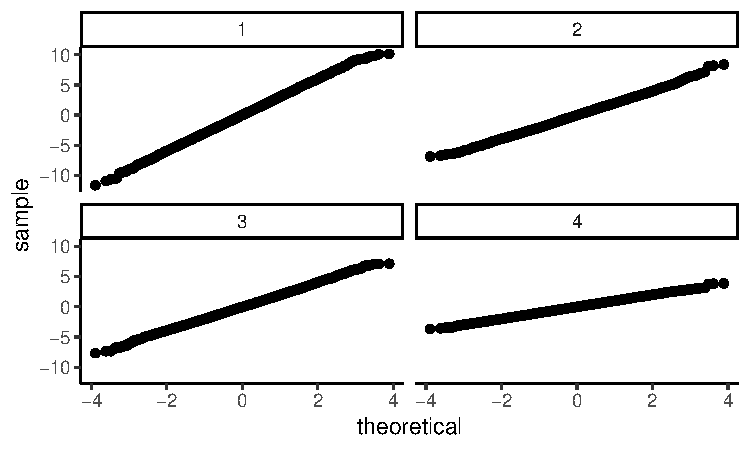
\includegraphics[width=0.75\linewidth]{Designing-Simulations-in-R_files/figure-latex/unnamed-chunk-67-1} \end{center}

We again check out.
Here, these checks may seem a bit silly, but most bugs are silly---at least once you find them!
It is easy for small things such as a sign error to happen once your model gets a bit more complex; even simple checks such as these can be quite helpful.

\section{Example: Simulating clustered data}\label{case-cluster}

Generating data with complex structure can be intimidating, but if you set out a recipe for how the data is generated it is often not to bad to build that recipe up with code.
We will next provide a more complex example with a case study of using simulation to determine best practices for analyzing data from a cluster-randomized RCT of students nested in schools.

Recent literature on multisite trials (where, for example, students are randomized to treatment or control within each of a series of sites) has explored how variation in the size of impacts across sites can affect how estimators behave, and what models we should use when there is impact variation (e.g., \citet{miratrix2021applied}, \citet{Bloom:2016um}).
We are going to extend this work to explore best practices for estimating treatment effects in cluster randomized trials.

Cluster randomized trials are randomized experiments where the unit of randomization is a group of individuals, rather than the individuals themselves.
For example, if we have a collection of schools, with students in schools, a cluster randomized trial would randomize the \emph{schools} into treatment or control, and then measure our outcome on the \emph{students} inside the schools.
We might be trying to estimate, for example, whether the average score of the treatment schools is different from the average score of the control schools.
In particular, we want to investigate what happens when the average treatment impact of a school is related to the size of the school.

Often we will design a data generating process to allow us to answer a specific question.
For our Welch example, we wanted to know how different amounts of variation in different groups impacted estimation.
We therefore needed a data generation process that allowed us to control that variation.
To figure out what we need for our clustered data example, we need to think about how we are going to use those data in our simulation study.

\subsection{A design decision: What do we want to manipulate?}\label{a-design-decision-what-do-we-want-to-manipulate}

There are a lot of ways we might generate cluster randomized trial data.
To pick between the many options, we need to think about the goals of the simulation.

Overall, our final data should be a collection of clusters with different sizes and different baseline mean outcomes.
Some of the clusters will be treated, and some not.
We can imagine our final data being individual students in schools, with each student having a school id, a treatment assignment (shared for all in the school) and an outcome.
A good starting point for building a DGP is to first write down a sketch of what the eventual data might look like on a piece of scratch paper.
In our case, for example, we might write down:

\begin{longtable}[]{@{}rrrrr@{}}
\toprule\noalign{}
schoolID & Z & size & studentID & Y \\
\midrule\noalign{}
\endhead
\bottomrule\noalign{}
\endlastfoot
1 & 1 & 24 & 1 & 3.6 \\
1 & 1 & 24 & 3 & 1.0 \\
1 & etc & etc & etc & etc \\
1 & 1 & 24 & 24 & 2.0 \\
2 & 0 & 32 & 1 & 0.5 \\
2 & 0 & 32 & 2 & 1.5 \\
2 & 0 & 32 & 3 & 1.2 \\
etc & etc & etc & etc & etc \\
\end{longtable}

We know we are planning on comparing multiple estimators, seeing how they behave differently under different conditions.
We also know that we are interested in what happens when the size of the treatment impact varies across sites, and in particular what happens when it is associated with site size.

Given these goals and beliefs, we might think:

\begin{enumerate}
\def\labelenumi{\arabic{enumi})}
\tightlist
\item
  We figure if all the sites are the same size, then all the estimators will probably be ok. But if sites vary, then maybe we could have issues with our estimators.
\item
  Also, if site size varies, but has nothing to do with impact, then all the estimators might still be ok, at least for bias, but if size is associated with treatment impact, then maybe how our estimators end up averaging across sites is going to matter.
\end{enumerate}

Usually, when running a simulation, it is good practice to test the simple option along with the complex one.
We want to both check that something does not matter as well as verify that it does.
Given this, we land on the following points:

\begin{itemize}
\tightlist
\item
  We need a DGP that has the option to make all-same-size sites or variable size sites.
\item
  Our DGP should have some impact variation across sites.
\item
  Our DGP should allow for different sites to have different treatment impacts.
\item
  We should have the option to connect impact variation to site size.
\end{itemize}

\subsection{A model for a cluster RCT}\label{a-model-for-a-cluster-rct}

It is usually easiest to start a recipe for data generating by writing down the mathematical model.
Write down something, and then, if you do not yet know how to generate some part of what you wrote down, specify how to generate those parts that you are using, in an iterative process.

For our model, we start with a model for our student outcome:

\[ Y_{ij} = \beta_{0j} + \epsilon_{ij} \mbox{ with } \epsilon_{ij} \sim N( 0, \sigma^2_\epsilon ) \]
where \(Y_{ij}\) is the outcome for student \(i\) in site \(j\), \(\beta_{0j}\) is the average outcome in site \(j\), and \(\epsilon_{ij}\) is the residual error for student \(i\) in site \(j\).

We then need to figure out how to make the average outcome in site \(j\).
In looking at our goals, we want \(\beta_{0j}\) to depend on treatment assignment.
We might then write down:

\[ \beta_{0j} = \gamma_0 + \gamma_1 Z_j + u_j \mbox{ with } u_j \sim N( 0, \sigma^2_u )\]
saying the average outcome in site \(j\) is the average outcome in the control group (\(\gamma_0\)) plus some treatment impact (\(\gamma_1\)) if the site is treated.
We added a \(u_j\) so that our different sites can be different from each other in terms of their average outcome, even if they are not treated.
To keep things simple, we are having a common treatment impact within cluster: if we treat a cluster, everyone in the cluster is raised by some specified amount.

But we also want the size of impact to possibly vary by site size.
This suggests we also want a treatment by site size interaction term.
Instead of just using the site size, however, we are going to standardize our site sizes so they are more interpretable.
This makes it so if we double the sizes of all the sites, it does not change our size covariate: we want the size covariate to be relative size, not absolute.
To do this, we create a covariate which is the percent of the average site size that a site is:
\[ S_j = \frac{n_j - \bar{n}}{ \bar{n} } \]

where \(\bar{n}\) is the average site size. Using this coveriate, we then revise our equation for our site \(j\) to:
\[ \beta_{0j} = \gamma_{0} + \gamma_{1} Z_j + \gamma_2 Z_j S_j + u_j \]
A nice thing about \(S_j\) is that it is centered at 0, meaning the average site has an impact of just \(\gamma_1\).
If \(S_j\) was not centered at zero, then our overall average impact in our data would be a mix of the \(\gamma_1\) and the \(\gamma_2\).
By centering, we make it so the average impact is just \(\gamma_1\)--\(\gamma_1\) is our target site average treatment impact.

If we put all the above together, we see we have specified a multilevel model to describe our data:
\[
\begin{aligned}
Y_{ij} &= \beta_{0j} + \epsilon_{ij} \\
\epsilon_{ij} &\sim N( 0, \sigma^2_\epsilon ) \\
\beta_{0j} &= \gamma_{0} + \gamma_{1} Z_j + \gamma_2 Z_j S_j + u_j \\
u_j &\sim N( 0, \sigma^2_u )
\end{aligned}
\]
Our parameters are the mean outcome of control unit (\(\gamma_0\)), the average treatment impact (\(\gamma_1\)), the amount of cross site variation (\(\sigma^2_u\)), and residual variation (\(\sigma^2_\epsilon\)).
Our \(\gamma_2\) is our site-size by treatment interaction term: bigger sites will (assuming \(\gamma_2\) is positive) have larger treatment impacts.

If you prefer the reduced form, it would be:

\[ Y_{ij} = \gamma_{0} + \gamma_{1} Z_j + \gamma_2 Z_j S_j  + u_j + \epsilon_{ij}  \]
We might also include a main effect for \(S_j\).
A main effect would make larger sites systematically different than smaller sites at baseline, rather than having it only be part of our treatment variation term.
For simplicity we drop it here.

In reviewing the above, we might notice that we do not have any variation in treatment impact that is not explained by site size.
We could once again revise our model to include a term for this, but we will leave it out for now.
See the exercises at the end of the chapter.

So far we have a mathematical model analogous to what we would write if we were \emph{analyzing} the data.
To \emph{generate} data, we also need several other quantities specified.
First, we need to know the number of clusters (\(J\)) and the sizes of the clusters (\(n_j\), for \(j = 1, \ldots, J\)).
We have to provide a recipe for generating these sizes.
We might try

\[ n_j \sim unif( (1-\alpha)\bar{n}, (1+\alpha)\bar{n} ) = \bar{n} + \bar{n}\alpha \cdot unif(-1, 1) ,\]
with a fixed \(\alpha\) to control the amount of variation in cluster size.
If \(\bar{n} = 100\) and \(\alpha = 0.25\) then we would, for example, have sites ranging from 75 to 125 in size.
This specification is nice in that we can determine two parameters, \(\bar{n}\) and \(\alpha\), to get our site sizes, and both parameters are easy to comprehend: average site size and amount of site size variation.

Given how we are generating site size, look again at our treatment impact heterogeneity term:

\[ \gamma_2 Z_j S_j = \gamma_2 Z_j \left(\frac{n_j - \bar{n}}{\bar{n}}\right) = \gamma_2 Z_j \alpha U_j, \]
where \(U_j\) is the \(U_j \sim unif(-1,1)\) uniform variable used to generate \(n_j\).
Due to our standardizing by average site size, we make our covariate not change in terms of its importance as a function of site size, but rather as a function of site variation \(\alpha\).
In particular, \(\frac{n_j - \bar{n}}{\bar{n}}\) will range from \(-\alpha\) to \(\alpha\), regardless of average site size.
Carefully setting up a DGP so the ``knobs'' we use are standardized like this can make interpreting the simulation results much easier.
Consider if we did not standardize and just had \(\gamma_2 n_j\) in our equation: in this case, for a set \(\gamma_2\), the overall average impact would grow if we changed the average site size, which could make interpreting the results across scenarios very confusing.
We generally want the parameters in our DGP to change only one aspect of our simulation, if possible, to make isolating effects of different DGP characteristics easier.

We next need to define how we generate our treatment indicator, \(Z_j\).
We might specify the proportion \(p\) of clusters we will assign to treatment, and then generate \(Z_j = 1\) or \(Z_j = 0\) using a simple random sampling approach on our \(J\) clusters.
We will see code for this below.

\subsection{Converting our model to code}\label{converting-our-model-to-code}

When sketching out our DGP mathematically we worked from the students to the schools.
For actual data generation, we will now follow our final model, but go by layers in the other direction.
First, we generate the sites:

\begin{itemize}
\tightlist
\item
  Generate site sizes
\item
  Generate site-level covariates
\item
  Generate site level random effects
\end{itemize}

Then we generate the students inside the sites:

\begin{itemize}
\tightlist
\item
  Generate student covariates
\item
  Generate student residuals
\item
  Add everything up to generate student outcomes
\end{itemize}

The mathematical model gives us exactly the details we need to execute on these steps.

We start by specifying a function with all the parameters we might want to pass it, including defaults for each (see \ref{default-arguments} for more on function defaults):

\begin{Shaded}
\begin{Highlighting}[]
\NormalTok{gen\_dat\_model }\OtherTok{\textless{}{-}} \ControlFlowTok{function}\NormalTok{( }\AttributeTok{n\_bar =} \DecValTok{10}\NormalTok{,}
                           \AttributeTok{J =} \DecValTok{30}\NormalTok{,}
                           \AttributeTok{p =} \FloatTok{0.5}\NormalTok{,}
                           \AttributeTok{gamma\_0 =} \DecValTok{0}\NormalTok{, }\AttributeTok{gamma\_1 =} \DecValTok{0}\NormalTok{, }\AttributeTok{gamma\_2 =} \DecValTok{0}\NormalTok{,}
                           \AttributeTok{sigma2\_u =} \DecValTok{0}\NormalTok{, }\AttributeTok{sigma2\_e =} \DecValTok{1}\NormalTok{,}
                           \AttributeTok{alpha =} \DecValTok{0}\NormalTok{ ) \{}
  \CommentTok{\# Code (see below) goes here.}
\NormalTok{\}}
\end{Highlighting}
\end{Shaded}

Note our parameters are a mix of \emph{model parameters} (\texttt{gamma\_0}, \texttt{gamma\_1}, \texttt{sigma2\_e}, etc., representing coefficients in regressions, variance terms, etc.) and \emph{design parameters} (\texttt{n\_bar}, \texttt{J}, \texttt{p}) that directly inform data generation.
We set default arguments (e.g., gamma\_0=0) so we can ignore aspects of the DGP that we do not care about later on.

Inside the model, we will have a block of code to generate the sites, and then another to generate the students.

\textbf{Make the sites.}
We make the sites first:

\begin{Shaded}
\begin{Highlighting}[]
  \CommentTok{\# generate site sizes }
\NormalTok{  n\_min }\OtherTok{=} \FunctionTok{round}\NormalTok{( n\_bar }\SpecialCharTok{*}\NormalTok{ (}\DecValTok{1} \SpecialCharTok{{-}}\NormalTok{ alpha) )}
\NormalTok{  n\_max }\OtherTok{=} \FunctionTok{round}\NormalTok{( n\_bar }\SpecialCharTok{*}\NormalTok{ (}\DecValTok{1} \SpecialCharTok{+}\NormalTok{ alpha) )}
\NormalTok{  nj }\OtherTok{\textless{}{-}} \FunctionTok{sample}\NormalTok{( n\_min}\SpecialCharTok{:}\NormalTok{n\_max, J, }\AttributeTok{replace=}\ConstantTok{TRUE}\NormalTok{ )}

  \CommentTok{\# Generate average control outcome and average ATE for all sites}
  \CommentTok{\# (The random effects)}
\NormalTok{  u0j }\OtherTok{=} \FunctionTok{rnorm}\NormalTok{( J, }\AttributeTok{mean=}\DecValTok{0}\NormalTok{, }\AttributeTok{sd=}\FunctionTok{sqrt}\NormalTok{( sigma2\_u ) )}
  
  \CommentTok{\# randomize units within each site (proportion p to treatment)}
\NormalTok{  Zj }\OtherTok{=} \FunctionTok{ifelse}\NormalTok{( }\FunctionTok{sample}\NormalTok{( }\DecValTok{1}\SpecialCharTok{:}\NormalTok{J ) }\SpecialCharTok{\textless{}=}\NormalTok{ J }\SpecialCharTok{*}\NormalTok{ p, }\DecValTok{1}\NormalTok{, }\DecValTok{0}\NormalTok{)}
  
  \CommentTok{\# Calculate site intercept for each site}
\NormalTok{  beta\_0j }\OtherTok{=}\NormalTok{ gamma\_0 }\SpecialCharTok{+}\NormalTok{ gamma\_1 }\SpecialCharTok{*}\NormalTok{ Zj }\SpecialCharTok{+}\NormalTok{ gamma\_2 }\SpecialCharTok{*}\NormalTok{ Zj }\SpecialCharTok{*}\NormalTok{ (nj}\SpecialCharTok{{-}}\NormalTok{n\_bar)}\SpecialCharTok{/}\NormalTok{n\_bar }\SpecialCharTok{+}\NormalTok{ u0j}
\end{Highlighting}
\end{Shaded}

The code is a literal translation of the math we did before.
Note the line with \texttt{sample(1:J)\ \textless{}=\ J*p}; this is a simple trick to generate a treatment and control 0/1 indicator.

There is also a serious error in the above code (serious in that the code will run and look fine in many cases, but not always do what we want); we leave it as an exercise (see below) to find and fix it.

\textbf{Make the individuals.}
We next use the site characteristics to then generate the individuals.

\begin{Shaded}
\begin{Highlighting}[]
  \CommentTok{\# Make individual site membership}
\NormalTok{  sid }\OtherTok{=} \FunctionTok{as.factor}\NormalTok{( }\FunctionTok{rep}\NormalTok{( }\DecValTok{1}\SpecialCharTok{:}\NormalTok{J, nj ) )}
\NormalTok{  dd }\OtherTok{=} \FunctionTok{data.frame}\NormalTok{( }\AttributeTok{sid =}\NormalTok{ sid )}
  
  \CommentTok{\# Make individual level tx variables}
\NormalTok{  dd}\SpecialCharTok{$}\NormalTok{Z }\OtherTok{=}\NormalTok{ Zj[ dd}\SpecialCharTok{$}\NormalTok{sid ]}
  
  \CommentTok{\# Generate the residuals }
\NormalTok{  N }\OtherTok{=} \FunctionTok{sum}\NormalTok{( nj )}
\NormalTok{  e }\OtherTok{=} \FunctionTok{rnorm}\NormalTok{( N, }\AttributeTok{mean=}\DecValTok{0}\NormalTok{, }\AttributeTok{sd=}\FunctionTok{sqrt}\NormalTok{( sigma2\_e ) )}
  
  \CommentTok{\# Bundle and send out}
\NormalTok{  dd }\OtherTok{\textless{}{-}} \FunctionTok{mutate}\NormalTok{( dd, }
                \AttributeTok{sid=}\FunctionTok{as.factor}\NormalTok{(sid),}
                \AttributeTok{Yobs =}\NormalTok{ beta\_0j[sid] }\SpecialCharTok{+}\NormalTok{ e, }
                \AttributeTok{Z =}\NormalTok{ Zj[ sid ] )}
\end{Highlighting}
\end{Shaded}

A key piece here is the \texttt{rep()} function that takes a list and repeats each element of the list a specified number of times.
In particular, \texttt{rep()} repeats each number (\(1, 2, /ldots,J\)), the corresponding number of times as listed in \texttt{nj}.

Once we put the above code in our function skeleton, we can our function as so:

\begin{Shaded}
\begin{Highlighting}[]
\NormalTok{dat }\OtherTok{\textless{}{-}} \FunctionTok{gen\_dat\_model}\NormalTok{( }\AttributeTok{n=}\DecValTok{5}\NormalTok{, }\AttributeTok{J=}\DecValTok{3}\NormalTok{, }\AttributeTok{p=}\FloatTok{0.5}\NormalTok{, }
                        \AttributeTok{gamma\_0=}\DecValTok{0}\NormalTok{, }\AttributeTok{gamma\_1=}\FloatTok{0.2}\NormalTok{, }\AttributeTok{gamma\_2=}\FloatTok{0.2}\NormalTok{,}
                        \AttributeTok{sigma2\_u =} \FloatTok{0.4}\NormalTok{, }\AttributeTok{sigma2\_e =} \DecValTok{1}\NormalTok{,}
                      \AttributeTok{alpha =} \FloatTok{0.5}\NormalTok{ )}

\NormalTok{dat}
\end{Highlighting}
\end{Shaded}

\begin{verbatim}
##    sid Z        Yobs
## 1    1 1  2.35779312
## 2    1 1  0.57601909
## 3    1 1  1.37583246
## 4    2 0 -0.04417977
## 5    2 0  0.35837270
## 6    2 0  2.43903900
## 7    2 0 -1.45205220
## 8    2 0 -1.05747062
## 9    2 0 -0.50122103
## 10   3 0 -0.25961309
## 11   3 0 -0.42459575
\end{verbatim}

Our data generation code is complete.
The next step is to test the code, making sure it is doing what we think it is.
See the exercises for more on this.

\section{Exercises}\label{exercises-1}

\subsection{\texorpdfstring{The Welch test on a shifted-and-scaled \(t\) distribution}{The Welch test on a shifted-and-scaled t distribution}}\label{ex_dgp}

The shifted-and-scaled \(t\)-distribution has parameters \(\mu\) (mean), \(\sigma\) (scale), and \(\nu\) (degrees of freedom).
If \(T\) follows a student's \(t\)-distribution with \(\nu\) degrees of freedom, then \(S = \mu + \sigma T\) follows a shifted-and-scaled \(t\)-distribution.

The following function will generate random draws from this distribution (the scaling of \((\nu-2)/\nu\) is to account for a non-scaled \(t\)-distribution having a variance of \(\nu/(\nu-2)\)).

\begin{Shaded}
\begin{Highlighting}[]
\NormalTok{r\_tss }\OtherTok{\textless{}{-}} \ControlFlowTok{function}\NormalTok{(n, mean, sd, df) \{}
\NormalTok{  mean }\SpecialCharTok{+}\NormalTok{ sd }\SpecialCharTok{*} \FunctionTok{sqrt}\NormalTok{( (df}\DecValTok{{-}2}\NormalTok{)}\SpecialCharTok{/}\NormalTok{df ) }\SpecialCharTok{*} \FunctionTok{rt}\NormalTok{(}\AttributeTok{n =}\NormalTok{ n, }\AttributeTok{df =}\NormalTok{ df)}
\NormalTok{\}}

\FunctionTok{r\_tss}\NormalTok{(}\AttributeTok{n =} \DecValTok{8}\NormalTok{, }\AttributeTok{mean =} \DecValTok{3}\NormalTok{, }\AttributeTok{sd =} \DecValTok{2}\NormalTok{, }\AttributeTok{df =} \DecValTok{5}\NormalTok{)}
\end{Highlighting}
\end{Shaded}

\begin{verbatim}
## [1]  4.6290066  3.3199535 -0.1054816  2.1896919
## [5]  2.4605947  0.1443433  1.0526101  1.9674069
\end{verbatim}

\begin{enumerate}
\def\labelenumi{\arabic{enumi}.}
\item
  Modify the Welch simulation's \texttt{simulate\_data()} function to generate data from shifted-and-scaled \(t\)-distributions rather than from normal distributions. Include the degrees of freedom as an input argument.
  Simulate a dataset with low degrees of freedom and plot it to see if you see a few outliers.
\item
  Now generate more data and calculate the means and standard deviations to see if they are correctly calibrated (generate a big dataset to ensure you get reliable mean and standard deviation estimates). Check \texttt{df} equal to 500, 5, 3, and 2.
\item
  Once you are satisfied you have a correct DGP function, re-run the Type-I error rate calculations from the prior exercises in Section \ref{exAnovaExercises} using a \(t\)-distribution with 5 degrees of freedom.
  Do the results change substantially?
\end{enumerate}

\subsection{Checking and extending the Cluster RCT DGP}\label{checking-and-extending-the-cluster-rct-dgp}

\begin{enumerate}
\def\labelenumi{\arabic{enumi}.}
\setcounter{enumi}{3}
\item
  What is the variance of the outcomes generated by our model if there is no treatment effect? (Try simulating data to check!) What other quick checks can you make on your DGP to make sure it is working?
\item
  In \texttt{gen\_dat\_model()} we have the following line of code to generate the number of individuals per site.
\end{enumerate}

\begin{Shaded}
\begin{Highlighting}[]
\NormalTok{nj }\OtherTok{\textless{}{-}} \FunctionTok{sample}\NormalTok{( n\_min}\SpecialCharTok{:}\NormalTok{n\_max, J, }
                 \AttributeTok{replace=}\ConstantTok{TRUE}\NormalTok{ )}
\end{Highlighting}
\end{Shaded}

This code has an error. Generate a variety of datasets where you vary \texttt{n\_min}, \texttt{n\_max} and \texttt{J} to discover the error. Then repair the code.
Checking your data generating process across a range of scenarios is extremely important.

\begin{enumerate}
\def\labelenumi{\arabic{enumi}.}
\setcounter{enumi}{5}
\item
  The DGP allows for site-level treatment impact variation--but only if it is related to site size. How could you modify your simulation to allow for site-level treatment impact variation that is not related to site size? Implement this change and generate some data to show how it works.
\item
  Extend the data generating process to include an individual level covariate \(X\) that is predictive of outcome. In particular, you will want to adjust your level one equation to
\end{enumerate}

\[ Y_{ij} = \beta_{0j} + \beta_{1} X_{ij} + \epsilon_{ij} . \]
Keep the same \(\beta_1\) for all sites.
You will have to specify how to generate your \(X_{ij}\).
For starters, just generate it as a standard normal, and do not worry about having the mean of \(X_{ij}\) vary by sites unless you are excited to try to get that to work.

\section{Extension: Standardization in a data generating process}\label{extension-standardization-in-a-data-generating-process}

In this chapter, we made a model to generate data for a cluster randomized trial.
Given our model, we can generate data by specifying our parameters and variables of \(\gamma_{0}, \gamma_{1}, \gamma_{2}, \sigma^2_\epsilon, \sigma^2_u, \bar{n}, \alpha, J, p\).

One factor that tends to show up when working with multisite data is how much variation there is within sites vs between sites.
For example, the Intra-Class Correlation (ICC), a measure of how much of the variation in the outcome is due to differences between sites, is a major component for power calculations.
Because of this, we will likely want to manipulate the amount of within vs.~between variation in our simulations.

An easy way to do this would be to simply raise or lower the amount of variation within sites (\(\sigma^2_u\)).
This unfortunately has a side effect: if we increase \(\sigma^2_u\), our overall variation of \(Y\) will also increase.
This will make it hard to think about, e.g., power, since we have confounded within vs.~between variation with overall variation (which is itself bad for power).
It also impacts interpretation of coefficients.
A treatment effect of 0.2 on our outcome scale is ``smaller'' if there is more overall variation.

Right now, our model is
\[ Y_{ij} = \gamma_{0} + \gamma_{1} Z_j + \gamma_2 Z_j \left(\frac{n_j - \bar{n}}{\bar{n}} \right)  + u_j + \epsilon_{ij}  \]

Given our model, the variance of our control-side outcomes is
\[ 
\begin{aligned}
var( Y_{ij}(0) ) &= var( \beta_{0j} + \epsilon_{ij} ) \\
 &= var( \gamma_{0} + \gamma_{1} Z_j + \gamma_{2}Z_j \tilde{n}_j + u_j + \epsilon_{ij} ) \\
&= \sigma^2_u + \sigma^2_\epsilon
\end{aligned}
\]
We see that as we increase either within or between variation, overall variation increases.

We can improve our data generating process to allow for directly controlling the amount of within vs.~between variation without it being confounded with overall variation.
To do this we first (1) Standardize our data and then (2) reparameterize, so we have human-selected parameters that we can interpret that we then \emph{translate} to our list of data generation parameters.
In particular, we will index our DGP with the more interpretable parameter of the Intra-Class Correlation (ICC), and standardize our DGP so it is all in effect size units.

The effect size of an impact is defined as the impact over the control-side standard deviation.
(Sometimes people use the pooled standard deviation, but this is usually a bad choice if one suspects treatment variation. More treatment variation should not reduce the effect size for the same absolute average impact.)

\[ ES = \frac{\gamma_1}{SD( Y | Z_j = 0 )} = \frac{\gamma_1}{\sqrt{ \sigma^2_u + \sigma^2_\epsilon } } \]

The way we think about how ``big'' \(\gamma_1\) is depends on how much site variation and residual variation there is.
But it is also easier to detect effects when the residual variation is small.
Effect sizes ``standardize out'' these sorts of tensions. We can use that.

In particular, we will use the Intraclass Correlation Coeffiicent (ICC), defined as
\[ ICC = \frac{ \sigma^2_u }{ \sigma^2_\epsilon + \sigma^2_u } . \]
The ICC is a measure of within vs.~between variation.

What we then do is first standardized our data, meaning we ensure the control side variance equals 1.
Using the above, this means \(\sigma^2_u + \sigma^2_\epsilon = 1\).
It also gives us \(ICC = \sigma^2_u\), and \(\sigma^2_\epsilon = 1 - ICC\).

Our two model parameters are now tied together by our single ICC tuning parameter.
The core idea is we can now manipulate the aspects of the DGP we want while holding other aspects of the DGP constant.
Given our standardized scale, we have dropped a parameter from our set of parameters we might want to vary, and ensured that varying the other parameter (now the ICC) is varying only one aspect of the DGP, not both.
Before, increasing \(\sigma^2_u\) had two consequences: total variation and relative amount of variation at the school level.
Now, manipulating ICC only does the latter.

E.g., we can call our DGP function as follows:

\begin{Shaded}
\begin{Highlighting}[]
\NormalTok{ICC }\OtherTok{=} \FloatTok{0.3}
\NormalTok{dat }\OtherTok{\textless{}{-}} \FunctionTok{gen\_dat\_model}\NormalTok{( }\AttributeTok{n\_bar =} \DecValTok{20}\NormalTok{, }\AttributeTok{J =} \DecValTok{30}\NormalTok{, }\AttributeTok{p =} \FloatTok{0.5}\NormalTok{,}
                      \AttributeTok{gamma\_0 =} \DecValTok{0}\NormalTok{, }\AttributeTok{gamma\_1 =} \FloatTok{0.3}\NormalTok{, }\AttributeTok{gamma\_2 =} \FloatTok{0.2}\NormalTok{,}
                      \AttributeTok{sigma2\_u =}\NormalTok{ ICC, }\AttributeTok{sigma2\_e =} \DecValTok{1} \SpecialCharTok{{-}}\NormalTok{ ICC,}
                      \AttributeTok{alpha =} \FloatTok{0.5}\NormalTok{ )}
\end{Highlighting}
\end{Shaded}

\chapter{Data analysis procedures}\label{data-analysis-procedures}

In the abstract, a function that implements an estimation procedure should have the following form:

\begin{Shaded}
\begin{Highlighting}[]
\NormalTok{estimate }\OtherTok{\textless{}{-}} \ControlFlowTok{function}\NormalTok{(data) \{}

  \CommentTok{\# calculations/model{-}fitting/estimation procedures}
  
  \FunctionTok{return}\NormalTok{(estimates)}
\NormalTok{\}}
\end{Highlighting}
\end{Shaded}

The function takes a data set as input, fits a model or otherwise calculates an estimate, possibly with associated standard errors and so forth, and produces as output these estimates.
In principle, you should be able to run your function on real data as well as simulated.

The estimates could be point-estimates of parameters, standard errors, confidence intervals, etc.
Depending on the research question, this function might involve a combination of several procedures (e.g., a diagnostic test for heteroskedasticity, followed by the conventional formula or heteroskedasticity-robust formula for standard errors).
Also depending on the research question, we might need to create \emph{several} functions that implement different estimation procedures to be compared.

In Chapter \ref{case-ANOVA}, for example, we saw different functions for some of the methods Brown and Forsythe considered for heteroskedastic ANOVA.

\section{Validating Estimation Procedures}\label{validating-estimation-procedures}

Just as with the data-generating function, it is important to verify the accuracy of the estimation functions.
For our Welch test, we can actually check our results against the built-in \texttt{oneway.test} function. Let's do that with a fresh set of data:

\begin{Shaded}
\begin{Highlighting}[]
\NormalTok{sim\_data }\OtherTok{\textless{}{-}} \FunctionTok{generate\_data}\NormalTok{(}\AttributeTok{mu =}\NormalTok{ mu, }\AttributeTok{sigma\_sq =}\NormalTok{ sigma\_sq,}
                          \AttributeTok{sample\_size =}\NormalTok{ sample\_size)}

\NormalTok{aov\_results }\OtherTok{\textless{}{-}} \FunctionTok{oneway.test}\NormalTok{(x }\SpecialCharTok{\textasciitilde{}} \FunctionTok{factor}\NormalTok{(group),}
                           \AttributeTok{data =}\NormalTok{ sim\_data, }
                           \AttributeTok{var.equal =} \ConstantTok{FALSE}\NormalTok{)}
\NormalTok{aov\_results}
\end{Highlighting}
\end{Shaded}

\begin{verbatim}
## 
##  One-way analysis of means (not assuming
##  equal variances)
## 
## data:  x and factor(group)
## F = 52.554, num df = 3.0000, denom df =
## 4.9584, p-value = 0.0003506
\end{verbatim}

\begin{Shaded}
\begin{Highlighting}[]
\NormalTok{Welch\_results }\OtherTok{\textless{}{-}} \FunctionTok{Welch\_F}\NormalTok{(sim\_data)}
\FunctionTok{all.equal}\NormalTok{(aov\_results}\SpecialCharTok{$}\NormalTok{p.value, Welch\_results)}
\end{Highlighting}
\end{Shaded}

\begin{verbatim}
## [1] TRUE
\end{verbatim}

We use \texttt{all.equal()} because it will check equality up to a tolerance in R, which can avoid some weird floating point errors due to rounding.

\section{Checking via simulation}\label{checking-via-simulation}

If your estimation procedure truly is new, how would you check it?
Well, one obvious answer is simulation!

In principle, for large samples and data generated under the assumptions required by your new procedure, you should have a fairly good sense that your estimation procedures should work.
It is often the case that as you design your simulation, and then start analyzing the results, you will find your estimators are really not working as planned.

Such surprises will usually be due to (at least) three factors: you did not implement your method correctly, your method is not yet a good idea in the first place, or you do not yet understand something important about how your method works.
When faced with poor performance you thus will debug your code, revise your method, and do some serious thinking.
Ideally this will eventually lead you to a deeper understanding of a method that is a better idea in general, and correctly implemented in all likelihood.

For example, in one research project Luke and other co-authors were working on a way to improve Instrumental Variable (IV) estimation using post-stratification.
The idea is to group units based on a covariate that predicts compliance status, and then estimate within each group; hopefully this would improve overall estimation.

In the first simulation, the estimates were full of NAs and odd results because we failed to properly account for what happens when the number of compliers was estimated to be zero.
That was table stakes: after repairing that, we still found odd behavior and serious and unexpected bias, which turned out to be due to failing to implement the averaging of the groups step correctly.
We fixed the estimator again and re-ran, and found that even when we had a variable that was almost perfectly predictive of compliance, gains were still surprisingly minimal.
Eventually we understood that the groups with very few compliers were actually so unstable that they ruined the overall estimate.
These results inspired us to introduce other estimators that dropped or down-weighted such strata, which gave our paper a deeper purpose and contribution.

Simulation is an iterative process.
It is to help you, the researcher, learn about your estimators so you can find a way forward with your work.
What you learn then feeds back to the prior research, and you have a cycle that you eventually step off of, if you want to finish your paper.
But do not expect it to be a single, well-defined, trajectory.

\section{Including Multiple estimation procedures}\label{including-multiple-estimation-procedures}

In Chapter \citet{data-generating-processes}, Section \ref{case-cluster} we introduced a case study of evaluating different procedures for estimating treatment impacts in a cluster randomized trial.
As a point of design, we generally recommend writing different functions for each estimation method one is planning on evaluating. This makes it easier to plug into play different methods as desired, and also helps generate a code base that is flexible and useful for other purposes.
It also, continuing our usual mantra, makes debugging easier: you can focus attention on one thing at a time, and worry less about how errors in one area might propagate to others.

For the cluster RCT context, we use two libraries, the \texttt{lme4} package (for multilevel modeling), the \texttt{arm} package (which gives us nice access to standard errors, with \texttt{se.fixef()}), and \texttt{lmerTest} (which gives us \(p\)-values for multilevel modeling).
We also need the \texttt{estimatr} package to get robust SEs with \texttt{lm\_robust}.
This use of different packages for different estimators is quite typical: in many simulations, many of the estimation approaches being considered are usually taken from the literature, and if you are lucky this means you can simply use a package that implements those methods.

We load our libraries at the top of our code:

\begin{Shaded}
\begin{Highlighting}[]
\FunctionTok{library}\NormalTok{( lme4 )}
\FunctionTok{library}\NormalTok{( arm )}
\FunctionTok{library}\NormalTok{( lmerTest )}
\FunctionTok{library}\NormalTok{( estimatr )}
\end{Highlighting}
\end{Shaded}

Our three analysis functions are then Multilevel Regression (MLM):

\begin{Shaded}
\begin{Highlighting}[]
\NormalTok{analysis\_MLM }\OtherTok{\textless{}{-}} \ControlFlowTok{function}\NormalTok{( dat ) \{}
\NormalTok{  M1 }\OtherTok{=} \FunctionTok{lmer}\NormalTok{( Yobs }\SpecialCharTok{\textasciitilde{}} \DecValTok{1} \SpecialCharTok{+}\NormalTok{ Z }\SpecialCharTok{+}\NormalTok{ (}\DecValTok{1}\SpecialCharTok{|}\NormalTok{sid),}
             \AttributeTok{data=}\NormalTok{dat )}
\NormalTok{  est }\OtherTok{=} \FunctionTok{fixef}\NormalTok{( M1 )[[}\StringTok{"Z"}\NormalTok{]]}
\NormalTok{  se }\OtherTok{=} \FunctionTok{se.fixef}\NormalTok{( M1 )[[}\StringTok{"Z"}\NormalTok{]]}
\NormalTok{  pv }\OtherTok{=} \FunctionTok{summary}\NormalTok{(M1)}\SpecialCharTok{$}\NormalTok{coefficients[}\StringTok{"Z"}\NormalTok{,}\DecValTok{5}\NormalTok{]}
  \FunctionTok{tibble}\NormalTok{( }\AttributeTok{ATE\_hat =}\NormalTok{ est, }\AttributeTok{SE\_hat =}\NormalTok{ se, }\AttributeTok{p\_value =}\NormalTok{ pv )}
\NormalTok{\}}
\end{Highlighting}
\end{Shaded}

Linear Regression with Cluster-Robust Standard Errors (LM):

\begin{Shaded}
\begin{Highlighting}[]
\NormalTok{analysis\_OLS }\OtherTok{\textless{}{-}} \ControlFlowTok{function}\NormalTok{( dat ) \{}
\NormalTok{  M2 }\OtherTok{\textless{}{-}} \FunctionTok{lm\_robust}\NormalTok{( Yobs }\SpecialCharTok{\textasciitilde{}} \DecValTok{1} \SpecialCharTok{+}\NormalTok{ Z, }
            \AttributeTok{data=}\NormalTok{dat, }\AttributeTok{clusters=}\NormalTok{sid )}
\NormalTok{  est }\OtherTok{\textless{}{-}}\NormalTok{ M2}\SpecialCharTok{$}\NormalTok{coefficients[[}\StringTok{"Z"}\NormalTok{]]}
\NormalTok{  se  }\OtherTok{\textless{}{-}}\NormalTok{ M2}\SpecialCharTok{$}\NormalTok{std.error[[}\StringTok{"Z"}\NormalTok{]]}
\NormalTok{  pv }\OtherTok{\textless{}{-}}\NormalTok{ M2}\SpecialCharTok{$}\NormalTok{p.value[[}\StringTok{"Z"}\NormalTok{]]}
  \FunctionTok{tibble}\NormalTok{( }\AttributeTok{ATE\_hat =}\NormalTok{ est, }\AttributeTok{SE\_hat =}\NormalTok{ se, }\AttributeTok{p\_value =}\NormalTok{ pv )}
\NormalTok{\}}
\end{Highlighting}
\end{Shaded}

and Aggregate data (Agg):

\begin{Shaded}
\begin{Highlighting}[]
\NormalTok{analysis\_agg }\OtherTok{\textless{}{-}} \ControlFlowTok{function}\NormalTok{( dat ) \{}
\NormalTok{  datagg }\OtherTok{\textless{}{-}} 
\NormalTok{    dat }\SpecialCharTok{\%\textgreater{}\%} 
    \FunctionTok{group\_by}\NormalTok{( sid, Z ) }\SpecialCharTok{\%\textgreater{}\%}
    \FunctionTok{summarise}\NormalTok{( }
      \AttributeTok{Ybar =} \FunctionTok{mean}\NormalTok{( Yobs ),}
      \AttributeTok{n =} \FunctionTok{n}\NormalTok{() }
\NormalTok{    )}
  
  \FunctionTok{stopifnot}\NormalTok{( }\FunctionTok{nrow}\NormalTok{( datagg ) }\SpecialCharTok{==} \FunctionTok{length}\NormalTok{(}\FunctionTok{unique}\NormalTok{(dat}\SpecialCharTok{$}\NormalTok{sid) ) )}
  
\NormalTok{  M3 }\OtherTok{\textless{}{-}} \FunctionTok{lm\_robust}\NormalTok{( Ybar }\SpecialCharTok{\textasciitilde{}} \DecValTok{1} \SpecialCharTok{+}\NormalTok{ Z, }
                   \AttributeTok{data=}\NormalTok{datagg, }\AttributeTok{se\_type =} \StringTok{"HC2"}\NormalTok{ )}
\NormalTok{  est }\OtherTok{\textless{}{-}}\NormalTok{ M3}\SpecialCharTok{$}\NormalTok{coefficients[[}\StringTok{"Z"}\NormalTok{]]}
\NormalTok{  se }\OtherTok{\textless{}{-}}\NormalTok{ M3}\SpecialCharTok{$}\NormalTok{std.error[[}\StringTok{"Z"}\NormalTok{]]}
\NormalTok{  pv }\OtherTok{\textless{}{-}}\NormalTok{ M3}\SpecialCharTok{$}\NormalTok{p.value[[}\StringTok{"Z"}\NormalTok{]]}
  \FunctionTok{tibble}\NormalTok{( }\AttributeTok{ATE\_hat =}\NormalTok{ est, }\AttributeTok{SE\_hat =}\NormalTok{ se, }\AttributeTok{p\_value =}\NormalTok{ pv )}
\NormalTok{\}}
\end{Highlighting}
\end{Shaded}

Note the \texttt{stopifnot} command: putting \emph{assert statements} in your code like this is a good way to guarantee you are not introducing weird and hard-to-track errors in your code.
For example, R likes to recycle vectors to make them the right length; if you gave it a wrong length in error, this can be a brutal error to discover.
The \texttt{stopifnot} statements halt your code as soon as something goes wrong, rather than letting that initial wrongness flow on to further work, showing up in odd results that you don't understand later on.
See Section \ref{about-stopifnot} for more.

All of our methods give output in the similar format:

\begin{Shaded}
\begin{Highlighting}[]
\FunctionTok{analysis\_MLM}\NormalTok{( dat )}
\end{Highlighting}
\end{Shaded}

\begin{verbatim}
## # A tibble: 1 x 3
##   ATE_hat SE_hat p_value
##     <dbl>  <dbl>   <dbl>
## 1   0.227  0.222   0.316
\end{verbatim}

\begin{Shaded}
\begin{Highlighting}[]
\FunctionTok{analysis\_OLS}\NormalTok{( dat )}
\end{Highlighting}
\end{Shaded}

\begin{verbatim}
## # A tibble: 1 x 3
##   ATE_hat SE_hat p_value
##     <dbl>  <dbl>   <dbl>
## 1   0.171  0.228   0.462
\end{verbatim}

\begin{Shaded}
\begin{Highlighting}[]
\FunctionTok{analysis\_agg}\NormalTok{( dat )}
\end{Highlighting}
\end{Shaded}

\begin{verbatim}
## # A tibble: 1 x 3
##   ATE_hat SE_hat p_value
##     <dbl>  <dbl>   <dbl>
## 1   0.232  0.222   0.305
\end{verbatim}

This will allow us to make our simulation, for each iteration, call each method in turn on the same dataset, stack the results into a small table, and return that result.
This will in turn get stacked to make one giant table of results, which makes evaluating performance quite easy.
We will see this in the next chapter.

\section{Exercises}\label{exercises-2}

\subsection{More Welch and adding the BFF test}\label{more-welch-and-adding-the-bff-test}

Let's continue to explore and tweak the simulation code we have developed to replicate the results of Brown and Forsythe (1974).

\begin{enumerate}
\def\labelenumi{\arabic{enumi}.}
\tightlist
\item
  Write a function that implements the Brown-Forsythe F*-test (the BFF* test!) as described on p.~130 of Brown and Forsythe (1974).
  Call it on a sample dataset to check it.
\end{enumerate}

\begin{Shaded}
\begin{Highlighting}[]
\NormalTok{BF\_F }\OtherTok{\textless{}{-}} \ControlFlowTok{function}\NormalTok{(x\_bar, s\_sq, n, g) \{}
  
  \CommentTok{\# fill in the guts here}
  
  \FunctionTok{return}\NormalTok{(pval)}
\NormalTok{\}}
\end{Highlighting}
\end{Shaded}

\begin{enumerate}
\def\labelenumi{\arabic{enumi}.}
\setcounter{enumi}{1}
\tightlist
\item
  Try calling your \texttt{BF\_F} function on a variety of datasets of different sizes and shapes, to make sure it works. What kinds of datasets should you test out?
\end{enumerate}

\subsection{More estimators for Cluster Randomized Trials}\label{more-estimators-for-cluster-randomized-trials}

\begin{enumerate}
\def\labelenumi{\arabic{enumi}.}
\setcounter{enumi}{2}
\tightlist
\item
  Sometimes you might want to consider two versions of an estimator. For example, in our cluster RCT code we used robust standard errors for the linear model estimator. Say we also want to include naive standard error estimates that we get out of the \texttt{lm} call.
\end{enumerate}

Extend the \texttt{OLS} call to be

\begin{verbatim}
analysis_OLS <- function( dat, robustSE = TRUE ) {
\end{verbatim}

and have the code inside calculate SEs based on the flag. Then modify the \texttt{analyze\_data()} to include both approaches (you will have to call \texttt{analysis\_OLS} twice).

\begin{enumerate}
\def\labelenumi{\arabic{enumi}.}
\setcounter{enumi}{3}
\tightlist
\item
  Efficiency-wise, estimating the OLS twice might not be ideal, but clarity-wise it might be considered helpful. Articulate two reasons for the design choice of implementing the two OLS calls separately, and articulate two reasons for instead having the \texttt{analysis\_OLS} method generate both standard errors internally in a single call.
\end{enumerate}

\chapter{Running the Simulation Process}\label{running-the-simulation-process}

In the prior two chapters we saw how to write functions that generate data according to a specified model (and parameters) and functions that implement estimation procedures on simulated data.
We next put those two together and repeat a bunch of times to obtain a lot of results such as point estimates, estimated standard errors and/or confidence intervals.

We use two primary ways of doing this in this textbook.
The first is to write a function that does a single step of a simulation, and then use the \texttt{map()} function to run that single step multiple times.

For our Cluster RCT case study, for example, we would write the following that takes our simulation parameters and runs a single trial of our simulation:

\begin{Shaded}
\begin{Highlighting}[]
\NormalTok{one\_run }\OtherTok{\textless{}{-}} \ControlFlowTok{function}\NormalTok{( }\AttributeTok{n\_bar =} \DecValTok{30}\NormalTok{, }\AttributeTok{J=}\DecValTok{20}\NormalTok{, }
                     \AttributeTok{gamma\_1 =} \FloatTok{0.3}\NormalTok{, }\AttributeTok{gamma\_2 =} \FloatTok{0.5}\NormalTok{,}
                     \AttributeTok{sigma2\_u =} \FloatTok{0.20}\NormalTok{, }\AttributeTok{sigma2\_e =} \FloatTok{0.80}\NormalTok{,}
                     \AttributeTok{alpha =} \FloatTok{0.75}\NormalTok{ ) \{}
  
\NormalTok{  dat }\OtherTok{\textless{}{-}} \FunctionTok{gen\_dat\_model}\NormalTok{( }\AttributeTok{n\_bar =}\NormalTok{ n\_bar, }\AttributeTok{J=}\NormalTok{J, }
                        \AttributeTok{gamma\_1 =}\NormalTok{ gamma\_1, }\AttributeTok{gamma\_2 =}\NormalTok{ gamma\_2,}
                        \AttributeTok{sigma2\_u =}\NormalTok{ sigma2\_u, }\AttributeTok{sigma2\_e =}\NormalTok{ sigma2\_e,}
                        \AttributeTok{alpha =}\NormalTok{ alpha )}
\NormalTok{  MLM }\OtherTok{=} \FunctionTok{analysis\_MLM}\NormalTok{( dat )}
\NormalTok{  LR }\OtherTok{=} \FunctionTok{analysis\_OLS}\NormalTok{( dat )}
\NormalTok{  Agg }\OtherTok{=} \FunctionTok{analysis\_agg}\NormalTok{( dat )}
  
  \FunctionTok{bind\_rows}\NormalTok{( }\AttributeTok{MLM =}\NormalTok{ MLM, }\AttributeTok{LR =}\NormalTok{ LR, }\AttributeTok{Agg =}\NormalTok{ Agg,}
             \AttributeTok{.id =} \StringTok{"method"}\NormalTok{ )}
\NormalTok{\}}
\end{Highlighting}
\end{Shaded}

We have added a bunch of defaults to our function, so we can easily run it without remembering all the things we can change.

When we call it, we get a nice table of results that we can evaluate:

\begin{Shaded}
\begin{Highlighting}[]
\FunctionTok{one\_run}\NormalTok{( }\AttributeTok{n\_bar =} \DecValTok{30}\NormalTok{, }\AttributeTok{J =} \DecValTok{20}\NormalTok{, }\AttributeTok{alpha=}\FloatTok{0.5}\NormalTok{ )}
\end{Highlighting}
\end{Shaded}

\begin{verbatim}
## # A tibble: 3 x 4
##   method  ATE_hat SE_hat p_value
##   <chr>     <dbl>  <dbl>   <dbl>
## 1 MLM     0.0450   0.192   0.818
## 2 LR     -0.00683  0.192   0.972
## 3 Agg     0.0580   0.193   0.768
\end{verbatim}

The results for each method is a single line.
We record estimated impact, estimated standard error, and a nominal \(p\)-value.
Note how the \texttt{bind\_rows()} method can take naming on the fly, and give us a column of \texttt{method}, which will be very useful for keeping track of what estimated what.
We intentionally wrap up our results with a data frame to make later processing of data with the tidyverse package much easier.

We then use the \texttt{map()} function to run this function multiple times:

\begin{Shaded}
\begin{Highlighting}[]
\FunctionTok{set.seed}\NormalTok{( }\DecValTok{40404}\NormalTok{ )}
\NormalTok{R }\OtherTok{=} \DecValTok{1000}
\NormalTok{ATE }\OtherTok{=} \FloatTok{0.30}
\NormalTok{runs }\OtherTok{\textless{}{-}} 
  \FunctionTok{map\_df}\NormalTok{( }\DecValTok{1}\SpecialCharTok{:}\NormalTok{R, }\SpecialCharTok{\textasciitilde{}}\FunctionTok{one\_run}\NormalTok{( }\AttributeTok{n\_bar =} \DecValTok{30}\NormalTok{, }\AttributeTok{J=}\DecValTok{20}\NormalTok{, }\AttributeTok{gamma\_1 =}\NormalTok{ ATE ),}
          \AttributeTok{.id=}\StringTok{"runID"}\NormalTok{ ) }

\FunctionTok{saveRDS}\NormalTok{( runs, }\AttributeTok{file =} \StringTok{"results/cluster\_RCT\_simulation.rds"}\NormalTok{ )}
\end{Highlighting}
\end{Shaded}

What the \texttt{map()} function is doing is first making a list from 1 to R, and then for each element in that list, it is calling \texttt{one\_run()} with the parameters \texttt{n\_bar\ =\ 30,\ J=20}.
The \texttt{\textasciitilde{}} is a shorthand way of writing a function that takes one argument, and then calls \texttt{one\_run()} with that argument; the argument is the iteration number (1, 2, 3, \ldots, R), but we are ignoring it. The \texttt{.id\ =\ "runID"} argument is a way of keeping track of which iteration number produced which result.
The \texttt{\_df} at the end of \texttt{map\_df()} is a way of telling \texttt{map()} to take the results of each iteration and bind them together into a single data frame.

Once our simulation is complete, we save our results to a file for future use; this speeds up our lives since we will not have to constantly re-run our simulation each time we want to explore the results.

We have arrived! We now have the individual results of all our methods applied to each of 1000 generated datasets.
The next step is to evaluate how well the estimators did.
Regarding our point estimate, for example, we have these primary questions:

\begin{itemize}
\tightlist
\item
  Is it biased? (bias)
\item
  Is it precise? (standard error)
\item
  Does it predict well? (RMSE)
\end{itemize}

In the next chapter, we systematically go through answering these questions for our initial scenario.

\section{Writing simulations quick with the simhelpers package}\label{writing-simulations-quick-with-the-simhelpers-package}

The \texttt{map} approach is a bit strange, with building a secret function on the fly with \texttt{\textasciitilde{}}, and also having the copy over all the parameters we pass from \texttt{one\_run()} to \texttt{gen\_dat\_model()}.
The \texttt{simhelpers} package provides a shortcut that makes this step easier.

To do it, we first need to write a single estimation procedure function that puts all of our estimators together:

\begin{Shaded}
\begin{Highlighting}[]
\NormalTok{analyze\_data }\OtherTok{=} \ControlFlowTok{function}\NormalTok{( dat ) \{}
\NormalTok{  MLM }\OtherTok{=} \FunctionTok{analysis\_MLM}\NormalTok{( dat )}
\NormalTok{  LR }\OtherTok{=} \FunctionTok{analysis\_OLS}\NormalTok{( dat )}
\NormalTok{  Agg }\OtherTok{=} \FunctionTok{analysis\_agg}\NormalTok{( dat )}
  
  \FunctionTok{bind\_rows}\NormalTok{( }\AttributeTok{MLM =}\NormalTok{ MLM, }\AttributeTok{LR =}\NormalTok{ LR, }\AttributeTok{Agg =}\NormalTok{ Agg,}
             \AttributeTok{.id =} \StringTok{"method"}\NormalTok{ )}
\NormalTok{\}}
\end{Highlighting}
\end{Shaded}

This is simply the \texttt{one\_run()} method from above, but without the data generating part.
When we pass a dataset to it, we get a nice table of results that we can evaluate, as we did before.

\begin{Shaded}
\begin{Highlighting}[]
\NormalTok{dat }\OtherTok{=} \FunctionTok{gen\_dat\_model}\NormalTok{( }\AttributeTok{n=}\DecValTok{30}\NormalTok{, }\AttributeTok{J =} \DecValTok{20}\NormalTok{, }\AttributeTok{gamma\_1 =} \FloatTok{0.30}\NormalTok{ )}
\FunctionTok{analyze\_data}\NormalTok{( dat )}
\end{Highlighting}
\end{Shaded}

\begin{verbatim}
## # A tibble: 3 x 4
##   method ATE_hat SE_hat  p_value
##   <chr>    <dbl>  <dbl>    <dbl>
## 1 MLM      0.517  0.119 0.000489
## 2 LR       0.509  0.122 0.000785
## 3 Agg      0.570  0.118 0.000138
\end{verbatim}

We can now use \texttt{simhelpers} to write us a new function for the entire simulation:

\begin{Shaded}
\begin{Highlighting}[]
\FunctionTok{library}\NormalTok{(simhelpers)}
\NormalTok{sim\_function }\OtherTok{\textless{}{-}} \FunctionTok{bundle\_sim}\NormalTok{( gen\_dat\_model, analyze\_data )}
\end{Highlighting}
\end{Shaded}

We can then use it as so:

\begin{Shaded}
\begin{Highlighting}[]
\FunctionTok{sim\_function}\NormalTok{( }\DecValTok{2}\NormalTok{, }\AttributeTok{n\_bar =} \DecValTok{30}\NormalTok{, }\AttributeTok{J =} \DecValTok{20}\NormalTok{, }\AttributeTok{gamma\_1 =}\NormalTok{ ATE )}
\end{Highlighting}
\end{Shaded}

\begin{verbatim}
## # A tibble: 6 x 4
##   method ATE_hat SE_hat  p_value
##   <chr>    <dbl>  <dbl>    <dbl>
## 1 MLM      0.533  0.128 0.000818
## 2 LR       0.519  0.134 0.00209 
## 3 Agg      0.662  0.295 0.0379  
## 4 MLM      0.326  0.116 0.0194  
## 5 LR       0.326  0.115 0.0153  
## 6 Agg      0.542  0.232 0.0312
\end{verbatim}

The \texttt{bundle\_sim()} command takes our DGP function and our estimation procedures function and gives us back a function, which we have called \texttt{sim\_function}, that will run a simulation using whatever parameters we give it.
The \texttt{bundle\_sim()} command examines \texttt{gen\_dat\_model} function, figures out what parameters it needs, and makes sure that the newly created function is able to take those parameters from the user.

To use it for our simulation, we would then write

\begin{Shaded}
\begin{Highlighting}[]
\NormalTok{rns }\OtherTok{\textless{}{-}} \FunctionTok{sim\_function}\NormalTok{( R, }\AttributeTok{n\_bar =} \DecValTok{30}\NormalTok{, }\AttributeTok{J =} \DecValTok{20}\NormalTok{, }\AttributeTok{gamma\_1 =}\NormalTok{ ATE )}
\FunctionTok{saveRDS}\NormalTok{( runs, }\AttributeTok{file =} \StringTok{"results/cluster\_RCT\_simulation.rds"}\NormalTok{ )}
\end{Highlighting}
\end{Shaded}

This is a bit more elegant than the \texttt{map()} approach, and is especially useful when we have a lot of parameters to pass around.

\section{Adding Checks and Balances}\label{adding-checks-and-balances}

In the extensions of the prior DGP chapter, we discussed indexing our DGP by the ICC instead of the two variance components.
We can do this, and also translate some of the more obscure model parameters to easier to interpret parameters from within our simulation driver as follows:

\begin{Shaded}
\begin{Highlighting}[]
\NormalTok{one\_run }\OtherTok{\textless{}{-}} \ControlFlowTok{function}\NormalTok{( }\AttributeTok{n\_bar =} \DecValTok{30}\NormalTok{, }\AttributeTok{J=}\DecValTok{20}\NormalTok{, }
                     \AttributeTok{ATE =} \FloatTok{0.3}\NormalTok{, }\AttributeTok{size\_coef =} \FloatTok{0.5}\NormalTok{,}
                     \AttributeTok{ICC =} \FloatTok{0.4}\NormalTok{,}
                     \AttributeTok{alpha =} \FloatTok{0.75}\NormalTok{ ) \{}
    \FunctionTok{stopifnot}\NormalTok{( ICC }\SpecialCharTok{\textgreater{}=} \DecValTok{0} \SpecialCharTok{\&\&}\NormalTok{ ICC }\SpecialCharTok{\textless{}} \DecValTok{1}\NormalTok{ )}

\NormalTok{  dat }\OtherTok{\textless{}{-}} \FunctionTok{gen\_dat\_model}\NormalTok{( }\AttributeTok{n\_bar =}\NormalTok{ n\_bar, }\AttributeTok{J=}\NormalTok{J, }
                        \AttributeTok{gamma\_1 =}\NormalTok{ ATE, }\AttributeTok{gamma\_2 =}\NormalTok{ size\_coef,}
                        \AttributeTok{sigma2\_u =}\NormalTok{ ICC, }\AttributeTok{sigma2\_e =} \DecValTok{1}\SpecialCharTok{{-}}\NormalTok{ICC,}
                        \AttributeTok{alpha =}\NormalTok{ alpha )}
\NormalTok{  MLM }\OtherTok{=} \FunctionTok{analysis\_MLM}\NormalTok{( dat )}
\NormalTok{  LR }\OtherTok{=} \FunctionTok{analysis\_OLS}\NormalTok{( dat )}
\NormalTok{  Agg }\OtherTok{=} \FunctionTok{analysis\_agg}\NormalTok{( dat )}
  
  \FunctionTok{bind\_rows}\NormalTok{( }\AttributeTok{MLM =}\NormalTok{ MLM, }\AttributeTok{LR =}\NormalTok{ LR, }\AttributeTok{Agg =}\NormalTok{ Agg,}
             \AttributeTok{.id =} \StringTok{"method"}\NormalTok{ )}
\NormalTok{\}}
\end{Highlighting}
\end{Shaded}

Note the \texttt{stopifnot}: it is wise to ensure our parameter transforms are all reasonable, so we do not get unexplained errors or strange results later on.
It is best if your code fails as soon as possible! Otherwise debugging can be quite hard.

In our modified \texttt{one\_run()} we are transforming our ICC parameter into specific other parameters that are used in our actual model to maintain our effect size interpretation of our simulation.
We have not even modified our \texttt{gen\_dat\_model()} DGP method: we are just specifying the constellation of parameters as a function of the parameters we want to directly control in the simulation.

Controlling how we use the foundational elements such as our data generating code is a key tool for making the higher level simulations sensible and more easily interpretable.
Here we have put our entire simulation into effect size units, and are now providing ``knobs'' to the simulation that are directly interpretable.

\section{Exercises}\label{exercises-3}

\begin{enumerate}
\def\labelenumi{\arabic{enumi}.}
\tightlist
\item
  In the prior chapter's exercises, you made a new \texttt{BF\_F} function for the Welch simulation. Now incorporate the \texttt{BF\_F} function into the \texttt{one\_run()} function, and use your revised function to generate simulation results for this additional estimator.
\end{enumerate}

\chapter{Performance criteria}\label{performance-criteria}

Once we have run our simulation, we have a pile of results to sort through.
Given these results, the question is now: how do we assess the performance of our evaluated estimation procedures?

In this chapter, we look at a variety of \textbf{performance criteria} that are commonly used to compare the relative performance of multiple estimators or measure how well an estimator works.
These performance criteria are all assessments of how the estimator behaves if you repeat the experimental process an infinite number of times.
In statistical terms, these criteria are summaries of the true sampling distribution of the estimator, given a specified data generating process.
For example, the bias of an estimator in a given scenario is how far off, on average, the estimator would be from the true parameter value if you repeated the experiment an infinite number of times.

Although we cannot observe the sampling distribution of an estimator directly (and it can only rarely be worked out in full mathematical detail), the set of estimates generated by a simulation constitute a (typically large) \emph{sample} from the sampling distribution of the studied estimator. (Say that six times fast!)
We can then use that sample to \emph{estimate} the performance criteria of interest.
For example, when we wanted to know what percent of the time we would reject the null hypothesis (for a given, specified situation) we estimated that by seeing how often we rejected in 1000 trials.

Now, because we have only a sample of trials rather than the full distribution, our estimates are merely estimates.
In other words, they can be wrong, just due to random chance.
We can describe how wrong with the \textbf{Monte Carlo standard error (MCSE)}.
The MCSE is the standard error of our estimate of performance due to the simulation only having a finite number of trials.
Just as with statistical uncertainty when analyzing data, we can estimate our MCSE and even use them to generate confidence intervals for our performance estimates.
The MCSE is \emph{not} related to the estimators being evaluated; the MCSE is a function of how much simulation we can do.
In a simulation study, we could, in theory, know \emph{exactly} how well our estimators do for a given context, if we ran an infinite number of simulations; the MCSE tells us how far we are from this ideal, given how many simulation trials we actually ran.
Given a desired MCSE, we could similarly determine how many replications were needed to ensure our performance estimates have a desired level of precision.

\section{Inference vs.~Estimation}\label{inference-vs.-estimation}

There are two general classes of analysis one typically does with data: inference and estimation.
To illustrate, we continue to reflect on the question of best practices for analyzing a cluster randomized experiment.
For this problem, we are focused on the \emph{estimand} of the site-average treatment effect, \(\gamma_1\).
The \emph{estimand} is the thing we are trying to estimate.
We can ask whether \(\gamma_1\) is non-zero (inference), and we can further ask what \(\gamma_1\) actually is (estimation).
More expanded we have:

\emph{Inference} is when we do hypothesis testing, asking whether there is evidence for some sort of effect, or asking whether there is evidence that some coefficient is greater than or less than some specified value.
In particular, for our example, to know if there is evidence that there is an average treatment effect at all we would test the null of \(H_0: \gamma_1 = 0\).

\emph{Estimation} is when we try to measure the size of an estimand such as an actual average treatment effect \(\gamma_1\).
Estimation has two major components, the point estimator and the uncertainty estimator.
We generally evaluate both the \emph{actual} properties of the point estimator and the performance of the \emph{estimated} properties of the point estimator.
For example, consider a specific estimate \(\hat{\gamma_1}\) of our average treatment effect.
We first wish to know the actual bias and true standard error (\(SE\)) of \(\hat{\gamma_1}\).
These are its actual properties.
However, for each estimated \(\hat{\gamma_1}\), we also estimate \(\widehat{SE}\), as our estimated measure of how precise our estimate is.
We need to understand the properties of \(\widehat{SE}\) as well.

Inference and estimation are clearly highly related--if we have a good estimate of the treatment effect and it is not zero, then we are willing to say that there is a treatment effect--but depending on the framing, the way you would set up a simulation to investigate the behavior of your estimators could be different.

\section{Ways of Assessing and Comparing Estimation Procedures}\label{ways-of-assessing-and-comparing-estimation-procedures}

We often have different methods for obtaining some estimate, and we often want to know which is best.
For example, comparison is the core question behind our running example of identifying which estimation strategy (aggregation, linear regression, or multilevel modeling) we should generally use when analyzing cluster randomized trial data.
The goal of a simulation comparing our estimators would be to identify whether our estimation strategies were different, whether one was superior to the other (and when), and what the salient differences were.
To fully understand the trade-offs and benefits, we would examine and compare the properties of our different approaches across a variety of circumstances, and with respect to a variety of metrics of success.

For inference, we first might ask whether our methods are valid, i.e., ask whether the methods work correctly when we test for a treatment effect when there is none.
For example, we might wonder whether using multilevel models could open the door to inference problems if we had model misspecification, such as in a scenario where the residuals had some non-normal distribution.
These sorts of questions are questions of validity.

Also for inference, we might ask which method is better for detecting an effect when there is one.
Here, we want to know how our estimators perform in circumstances with a non-zero average treatment effect.
Do they reject the null often, or rarely?
How much does using aggregation decrease (or increase?) our chances of rejection?
These are questions about power.

For estimation, we generally are concerned with two things: bias and variance.
An estimator is biased if it would generally give estimates that are systematically higher (or lower) than the parameter being estimated in a given scenario.
The variance of an estimator is a measure of how much the estimates vary from trial to trial.
The variance is the true standard error, squared.

We might also be concerned with how well we can estimate the uncertainty of our estimators (i.e., estimate our standard error).
For example, we might have an estimator that works very well, but we have no ability to estimate how well.
Continuing our example, we might want to examine how well, for example, the standard errors we get from aggregation work as compared to the standard errors we get out of our linear regression approach.

Finally, we might want to know how well confidence intervals based on our methods work.
Do the intervals capture the true estimands with the desired level of accuracy, across the simulation trials?
Are the intervals for one method generally shorter or longer than those of another?

\section{Assessing a Point Estimator}\label{assessing-a-point-estimator}

Assessing the actual properties of a point estimator is generally fairly simple.
For a given scenario, repeatedly generate data and estimate effects.
Then take summary measures such as the mean and standard deviation of these repeated trials' estimates to estimate the actual properties of the estimator via Monte Carlo.
Given sufficient simulation trials, we can obtain arbitrarily accurate measures.

The most common measures of an estimator are the bias, variance, and mean squared error.
For example, we can ask what the \emph{actual} variance (or standard error) of our estimator is.
We can ask if our estimator is biased.
We can ask what the overall \(RMSE\) (root mean squared error) of our estimator is.

To be more formal, consider an estimator \(T\) that is targeting a parameter \(\theta\).
A simulation study generates a (typically large) sample of estimates \(T_1,...,T_R\), all of the target \(\theta\).
We know \(\theta\) because we generated the data.

We can first assess whether our estimator is biased, by comparing the mean of our \(R\) estimates
\[ \bar{T} = \frac{1}{R}\sum_{r=1}^R T_r \]
to \(\theta\).
The bias of our estimator is \(bias = \bar{T} - \theta\).

We can also ask how variable our estimator is, by calculating the variance of our \(R\) estimates
\[\displaystyle{S_T^2 = \frac{1}{R - 1}\sum_{r=1}^R \left(T_r - \bar{T}\right)^2} . \]

The square root of this, \(S_T\) is the true standard error of our estimator (up to Monte Carlo simulation uncertainty).

Finally, the Root Mean Square Error (RMSE) is a combination of the above two measures:
\[ RMSE = \left\{ \frac{1}{R} \sum_{r = 1}^R \left( T_r - \theta\right)^2 \right\}^{1/2}. \]
Often people talk about the MSE (Mean Squared Error)--this is just the RMSE squared.

An important relationship connecting these three measures is
\[ RMSE^2 = bias^2 + variance = bias^2 + SE^2 .\]
It is important to clarify an important point: the \emph{true standard error} of an estimator \(\hat{\gamma_1}\) is the standard deviation of \(\hat{\gamma_1}\) across multiple datasets.
In practice, we never know this value, but in a simulation we can obtain it as the standard deviation of our simulation trial estimates.
People generally, when they say ``Standard Error'' mean \emph{estimated} Standard Error, (\(\widehat{SE}\)) which is when one uses the emperical data to estimate \(SE\).
For assessing actual properties, we have the true standard error (up to Monte Carlo simulation error).

For absolute assessments of performance, an estimator with low bias, low variance, and thus low RMSE is desired.
For comparisons of relative performance, an estimator with lower RMSE is usually preferable to an estimator with higher RMSE; if two estimators have comparable RMSE, then the estimator with lower bias would usually be preferable.

It is important to recognize that the above performance measures depend on the scale of the parameter.
For example, if our estimators are measuring a treatment impact in dollars, then our bias, SE, and RMSE are all in dollars.
The variance and MSE would be in dollars squared, which is why we take their square roots to put them back on an intepretable dollars scale.

Usually in a simulation, the scale of the outcome is irrelevant as we are comparing one estimator to the other.
To ease interpretation, we might want to assess estimators relative to the baseline variation.
To achieve this, we can generate data so the outcome has unit variance (i.e., we generate \emph{standardized data}).
Then the bias, median bias, and root mean-squared error would all be in standard deviation units.

By contrast, a nonlinear change of scale of a parameter can lead to nonlinear changes in the performance measures.
For instance, suppose that \(\theta\) is a measure of the proportion of time that a behavior occurs.
A natural way to transform this parameter would be to put it on the log-odds (logit) scale.
However, because of the nonlinear aspect of the logit,
\[\text{Bias}\left[\text{logit}(T)\right] \neq \text{logit}\left(\text{Bias}[T]\right), \qquad \text{RMSE}\left[\text{logit}(T)\right] \neq \text{logit}\left(\text{RMSE}[T]\right),\]
and so on.
This is fine, but one should be aware that this can happen and do it on purpose.

\subsection{Comparing the Performances of the Cluster RCT Estimation Procedures}\label{comparing-the-performances-of-the-cluster-rct-estimation-procedures}

Given our simulation results generated in the last chapter, we next assess the bias, standard error, and RMSE of our three different estimators of the ATE.
These performance criteria address these primary questions:

\begin{itemize}
\tightlist
\item
  Is the estimator systematically off? (bias)
\item
  Is it precise? (standard error)
\item
  Does it predict well? (RMSE)
\end{itemize}

Let us see how the three estimators compare on these criteria.

\textbf{Are the estimators biased?}
Bias is with respect to a target estimand.
Here we assess whether our estimates are systematically different from the \(\gamma_1\) parameter we used to generate the data (this is the ATE parameter, which we had set to 0.30).

\begin{Shaded}
\begin{Highlighting}[]
\NormalTok{runs }\SpecialCharTok{\%\textgreater{}\%} 
  \FunctionTok{group\_by}\NormalTok{( method ) }\SpecialCharTok{\%\textgreater{}\%}
  \FunctionTok{summarise}\NormalTok{( }
    \AttributeTok{mean\_ATE\_hat =} \FunctionTok{mean}\NormalTok{( ATE\_hat ),}
    \AttributeTok{bias =} \FunctionTok{mean}\NormalTok{( ATE\_hat }\SpecialCharTok{{-}}\NormalTok{ ATE )  )}
\end{Highlighting}
\end{Shaded}

\begin{verbatim}
## # A tibble: 3 x 3
##   method mean_ATE_hat    bias
##   <chr>         <dbl>   <dbl>
## 1 Agg           0.306 0.00561
## 2 LR            0.390 0.0899 
## 3 MLM           0.308 0.00788
\end{verbatim}

Linear regression, with a bias of about 0.09 effect size units, appears about ten times as biased as the other estimators.
There is no evidence of major bias for Agg or MLM.
This is because the linear regression is targeting the person-average average treatment effect.
Our data generating process makes larger sites have larger effects, so the person average is going to be higher since those larger sites will count more.
Our estimand, by contrast, is the site average treatment effect, i.e., the simple average of each site's true impact, which our DGP has set to 0.30.
The Agg and MLM methods, by contrast, estimate this site-average effect, putting them in line with our DGP.

If we had instead decided our target estimand was the person average effect, then we would see linear regression as unbiased, and Agg and MLM as biased; it is important to think carefully about what the estimators are targeting, and report bias with respect to a clearly articulated goal.

\textbf{Which method has the smallest standard error?}
The true Standard Error is simply how variable a point estimator is, and is calculated as the standard deviation of the point estimates for a given estimator.
The Standard Error reflects how stable our estimates are across datasets that all came from the same data generating process.
We calculate the standard error, and also the relative standard error using linear regression as a baseline:

\begin{Shaded}
\begin{Highlighting}[]
\NormalTok{true\_SE }\OtherTok{\textless{}{-}}\NormalTok{ runs }\SpecialCharTok{\%\textgreater{}\%} 
  \FunctionTok{group\_by}\NormalTok{( method ) }\SpecialCharTok{\%\textgreater{}\%}
  \FunctionTok{summarise}\NormalTok{( }
    \AttributeTok{SE =} \FunctionTok{sd}\NormalTok{( ATE\_hat )}
\NormalTok{  )}
\NormalTok{true\_SE }\SpecialCharTok{\%\textgreater{}\%}
  \FunctionTok{mutate}\NormalTok{( }\AttributeTok{per\_SE =}\NormalTok{ SE }\SpecialCharTok{/}\NormalTok{ SE[method}\SpecialCharTok{==}\StringTok{"LR"}\NormalTok{] )}
\end{Highlighting}
\end{Shaded}

\begin{verbatim}
## # A tibble: 3 x 3
##   method    SE per_SE
##   <chr>  <dbl>  <dbl>
## 1 Agg    0.168  0.916
## 2 LR     0.183  1    
## 3 MLM    0.168  0.916
\end{verbatim}

These standard errors are all what we would be trying to estimate with a standard error estimator in a normal data analysis.
The other methods appear to have SEs about 8\% smaller than Linear Regression.

\textbf{Which method has the smallest Root Mean Squared Error?}

So far linear regression is not doing well: it has more bias and a larger standard error than the other two.
We can assess overall performance by combining these two quantities with the RMSE:

\begin{Shaded}
\begin{Highlighting}[]
\NormalTok{runs }\SpecialCharTok{\%\textgreater{}\%} 
  \FunctionTok{group\_by}\NormalTok{( method ) }\SpecialCharTok{\%\textgreater{}\%}
  \FunctionTok{summarise}\NormalTok{( }
    \AttributeTok{bias =} \FunctionTok{mean}\NormalTok{( ATE\_hat }\SpecialCharTok{{-}}\NormalTok{ ATE ),}
    \AttributeTok{SE =} \FunctionTok{sd}\NormalTok{( ATE\_hat ),}
    \AttributeTok{RMSE =} \FunctionTok{sqrt}\NormalTok{( }\FunctionTok{mean}\NormalTok{( (ATE\_hat }\SpecialCharTok{{-}}\NormalTok{ ATE)}\SpecialCharTok{\^{}}\DecValTok{2}\NormalTok{ ) )}
\NormalTok{  ) }\SpecialCharTok{\%\textgreater{}\%}
  \FunctionTok{mutate}\NormalTok{( }\AttributeTok{per\_RMSE =}\NormalTok{ RMSE }\SpecialCharTok{/}\NormalTok{ RMSE[method}\SpecialCharTok{==}\StringTok{"LR"}\NormalTok{] )}
\end{Highlighting}
\end{Shaded}

\begin{verbatim}
## # A tibble: 3 x 5
##   method    bias    SE  RMSE per_RMSE
##   <chr>    <dbl> <dbl> <dbl>    <dbl>
## 1 Agg    0.00561 0.168 0.168    0.823
## 2 LR     0.0899  0.183 0.204    1    
## 3 MLM    0.00788 0.168 0.168    0.823
\end{verbatim}

We also include SE and bias as reference.

RMSE is a way of taking both bias and variance into account, all at once.
For Agg and MLM, the RMSE is basically the standard error; this makes sense as they are not biased.
For LR, the combination of bias plus increased variability gives a higher RMSE.
That said, clearly the standard error dominates the bias term (note how RMSE and SE are more similar than RMSE and bias).
This is especially the case as RMSE is the square root of the bias and standard errors \emph{squared}; this makes difference between them even more extreme.
Overall, Agg and MLM have RMSEs around 16\% smaller than LR--this seems notable.

\subsection{Handling Estimands Not Represented By a Parameter}\label{handling-estimands-not-represented-by-a-parameter}

In our Cluster RCT example, we have focused on an estimand of the ATE as captured by our model parameter \(\gamma_1\).
But say we were interested in the person-average effect.
This is not represented by any number, so we would have to calculate it and then compare all of our estimates to it.

We offer two ways of doing this.
The first is to simply generate a massive dataset, and then average across it to get a good estimate of the true person-average effect.
If our dataset is big enough, then the uncertainty in this estimate will be neglidgable compared to the uncertainty in our simulation.

Here we try this:

\begin{Shaded}
\begin{Highlighting}[]
\NormalTok{dat }\OtherTok{=} \FunctionTok{gen\_dat\_model}\NormalTok{( }\AttributeTok{n\_bar =} \DecValTok{30}\NormalTok{, }\AttributeTok{J=}\DecValTok{100000}\NormalTok{, }
                     \AttributeTok{gamma\_1 =} \FloatTok{0.3}\NormalTok{, }\AttributeTok{gamma\_2 =} \FloatTok{0.5}\NormalTok{,}
                     \AttributeTok{sigma2\_u =} \FloatTok{0.20}\NormalTok{, }\AttributeTok{sigma2\_e =} \FloatTok{0.80}\NormalTok{,}
                     \AttributeTok{alpha =} \FloatTok{0.75}\NormalTok{  )}
\NormalTok{ATE\_person }\OtherTok{=} \FunctionTok{mean}\NormalTok{( dat}\SpecialCharTok{$}\NormalTok{Yobs[dat}\SpecialCharTok{$}\NormalTok{Z}\SpecialCharTok{==}\DecValTok{1}\NormalTok{] ) }\SpecialCharTok{{-}} \FunctionTok{mean}\NormalTok{( dat}\SpecialCharTok{$}\NormalTok{Yobs[dat}\SpecialCharTok{$}\NormalTok{Z}\SpecialCharTok{==}\DecValTok{0}\NormalTok{] )}
\NormalTok{ATE\_person}
\end{Highlighting}
\end{Shaded}

\begin{verbatim}
## [1] 0.3920888
\end{verbatim}

Note our estimate of the person-average effect of 0 is about what we would expect given the bias of the linear model!

Note how bias and RMSE have shifted, but SE is the same, when we compare to \texttt{ATE\_person}:

\begin{Shaded}
\begin{Highlighting}[]
\NormalTok{runs }\SpecialCharTok{\%\textgreater{}\%} 
  \FunctionTok{group\_by}\NormalTok{( method ) }\SpecialCharTok{\%\textgreater{}\%}
  \FunctionTok{summarise}\NormalTok{( }
    \AttributeTok{bias =} \FunctionTok{mean}\NormalTok{( ATE\_hat }\SpecialCharTok{{-}}\NormalTok{ ATE\_person ),}
    \AttributeTok{SE =} \FunctionTok{sd}\NormalTok{( ATE\_hat ),}
    \AttributeTok{RMSE =} \FunctionTok{sqrt}\NormalTok{( }\FunctionTok{mean}\NormalTok{( (ATE\_hat }\SpecialCharTok{{-}}\NormalTok{ ATE\_person)}\SpecialCharTok{\^{}}\DecValTok{2}\NormalTok{ ) )}
\NormalTok{  ) }\SpecialCharTok{\%\textgreater{}\%}
  \FunctionTok{mutate}\NormalTok{( }\AttributeTok{per\_RMSE =}\NormalTok{ RMSE }\SpecialCharTok{/}\NormalTok{ RMSE[method}\SpecialCharTok{==}\StringTok{"LR"}\NormalTok{] )}
\end{Highlighting}
\end{Shaded}

\begin{verbatim}
## # A tibble: 3 x 5
##   method     bias    SE  RMSE per_RMSE
##   <chr>     <dbl> <dbl> <dbl>    <dbl>
## 1 Agg    -0.0865  0.168 0.189     1.03
## 2 LR     -0.00222 0.183 0.183     1   
## 3 MLM    -0.0842  0.168 0.188     1.02
\end{verbatim}

We see Agg and MLM are now biased, and LR is unbiased.
RMSE is now a tension between bias and reduced variance.
Overall, Agg and MLM are 4\% worse than LR in terms of RMSE, because they have lower SEs but more bias.

The second method of calculating \texttt{ATE\_person} would be to record the true person average effect of the dataset of each simulation iteration, and then average those at the end.
To do this we would need to modify our \texttt{gen\_dat\_model()} DGP code to track this additional information.
We might have, for example

\begin{Shaded}
\begin{Highlighting}[]
\NormalTok{tx\_effect }\OtherTok{=}\NormalTok{ gamma\_1 }\SpecialCharTok{+}\NormalTok{ gamma\_2 }\SpecialCharTok{*}\NormalTok{ (nj}\SpecialCharTok{{-}}\NormalTok{n\_bar)}\SpecialCharTok{/}\NormalTok{n\_bar}
\NormalTok{beta\_0j }\OtherTok{=}\NormalTok{ gamma\_0 }\SpecialCharTok{+}\NormalTok{ Zj }\SpecialCharTok{*}\NormalTok{ tx\_effect }\SpecialCharTok{+}\NormalTok{ u0j}
\end{Highlighting}
\end{Shaded}

and then we would return \texttt{tx\_effect} as well as \texttt{Yobs} and \texttt{Z} as a column in our dataset.
This is similar to directly calculating \emph{potential outcomes}, as discussed in Chapter \ref{chap-potential-outcomes}.

Once we modified our DGP code, we \emph{also} need to modify our analysis functions to record this information.
We might have, for example:

\begin{Shaded}
\begin{Highlighting}[]
\NormalTok{analyze\_data }\OtherTok{=} \ControlFlowTok{function}\NormalTok{( dat ) \{}
\NormalTok{  MLM }\OtherTok{=} \FunctionTok{analysis\_MLM}\NormalTok{( dat )}
\NormalTok{  LR }\OtherTok{=} \FunctionTok{analysis\_OLS}\NormalTok{( dat )}
\NormalTok{  Agg }\OtherTok{=} \FunctionTok{analysis\_agg}\NormalTok{( dat )}
\NormalTok{  res }\OtherTok{\textless{}{-}} \FunctionTok{bind\_rows}\NormalTok{( }\AttributeTok{MLM =}\NormalTok{ MLM, }\AttributeTok{LR =}\NormalTok{ LR, }\AttributeTok{Agg =}\NormalTok{ Agg,}
             \AttributeTok{.id =} \StringTok{"method"}\NormalTok{ )}
\NormalTok{  res}\SpecialCharTok{$}\NormalTok{ATE\_person }\OtherTok{=} \FunctionTok{mean}\NormalTok{( dat}\SpecialCharTok{$}\NormalTok{tx\_effect )}
  \FunctionTok{return}\NormalTok{( res )}
\NormalTok{\}}
\end{Highlighting}
\end{Shaded}

Now when we run our simulation, we would have a column which is the true person average treatment effect for each dataset.
We could then take the average of those across our datasets to estimate the true person average treatment effect in the population, and then compare our point estimators to that value.

Clearly, an estimand that is not represented by a parameter is more difficult to work with, but it is not impossible.
As always, be clear as to what you are trying to estimate.

\section{Assessing a Standard Error Estimator}\label{assessing-a-standard-error-estimator}

Statistics is perhaps more about assessing how good an estimate is than making an estimate in the first place.
This translates to simulation studies: in our simulation we can know an estimator's actual properties, but if we were to use this estimator in practice we would have to also estimate its associated standard error, and generate confidence intervals and so forth using this standard error estimate.
To understand if this would work in practice, we would need to evaluate not only the behavior of the estimator itself, but the behavior of these associated things.
In other words, we generally not only want to know whether our point estimator is doing a good job, but we usually want to know whether we are able to get a good standard error for that point estimator as well.

To do this we first compare the expected value of \(\widehat{SE}\) (estimated with the average \(\widehat{SE}\) across our simulation trials) to the actual \(SE\).
This tells us whether our uncertainty estimates are \emph{biased}.
We could also examine the standard deviation of \(\widehat{SE}\) across trials, which tells us whether our estimates of uncertainty are relatively stable.
We finally could examine whether there is correlation between \(\widehat{SE}\) and the actual error (e.g., \(\left|T - \theta \right|\)).
Good estimates of uncertainty should predict error in a given context (especially if calculating conditional estimates); see \citet{sundberg2003conditional}.

For the first assessment, we usually assess the quality of a standard error estimator with a relative performance criteria, rather than an absolute one, meaning we compare the estimated standard error to the true standard error as a ratio.

For an example, suppose that in our simulation we are examining the performance of a point-estimator \(T\) for a parameter \(\theta\) along with an estimator \(\widehat{SE}\) for the standard error of \(T\).
In this case, we likely do not know the true standard error of \(T\), for our simulation context, prior to the simulation.
However, we can use the variance of \(T\) across the replications (\(S_T^2\)) to directly estimate the true sampling variance \(\text{Var}(T) = SE^2(T)\).
The \emph{relative bias} of \(\widehat{SE}^2\) would then be estimated by \(RB = \bar{V} / S_T^2\), where \(\bar{V}\) is the average of \(\widehat{SE}^2\) across simulation runs.
Note that a value of 1 for relative bias corresponds to exact unbiasedness of the variance estimator.
The relative bias measure is a measure of \emph{proportionate} under- or over-estimation.
For example, a relative bias of 1.12 would mean the standard error was, on average, 12\% too large.
We discuss relative performance measures further in Section \ref{sec-relative-performance}.

\subsection{Why Not Assess the Estimated SE directly?}\label{why-not-assess-the-estimated-se-directly}

We typically see assessment of \(\widehat{SE}^2\), not \(\widehat{SE}\).
In other words, we typically work with assessing whether the variance estimator is unbiased, etc., rather than the standard error estimator.
This comes out of a few reasons.
First, in practice, so-called unbiased standard errors usually are not in fact actually unbiased (see the delightfully titled section 11.5, ``The Joke Is on Us: The Standard Deviation Estimator is Biased after All,'' in \citet{westfall2013understanding} for further discussion).
For linear regression, for example, the classic standard error estimator is an unbiased \emph{variance} estimator, meaning that we have a small amount of bias due to the square-rooting because:

\[ E[ \sqrt{ V } ] \neq \sqrt{ E[ V ] } . \]

Variance is also the component that gives us the classic bias-variance breakdown of \(MSE = Variance + Bias^2\), so if we are trying to assign whether an overall MSE is due to instability or systematic bias, operating in this squared space may be preferable.

That being said, to put things in terms of performance criteria humans understand, it is usually nicer to put final evaluation metrics back into standard error units.
For example, saying there is a 10\% reduction in the standard error is more meaningful (even if less impressive sounding) than saying there is a 19\% reduction in the variance.

\subsection{Assessing SEs for Our Cluster RCT Simulation}\label{assessing-ses-for-our-cluster-rct-simulation}

To assess whether our estimated SEs are about right, we can look at the average \emph{estimated} (squared) standard error and compare it to the true standard error.
Our standard errors are \emph{inflated} if they are systematically larger than they should be, across the simulation runs.
We can also look at how stable our standard error estimates are, by taking the standard deviation of our standard error estimates.
We interpret this quantity relative to the actual standard error to get how far off, as a percent of the actual standard error, we tend to be.

\begin{Shaded}
\begin{Highlighting}[]
\NormalTok{runs }\SpecialCharTok{\%\textgreater{}\%}  \FunctionTok{group\_by}\NormalTok{( method ) }\SpecialCharTok{\%\textgreater{}\%}
  \FunctionTok{summarise}\NormalTok{( }
    \AttributeTok{SE =} \FunctionTok{sd}\NormalTok{( ATE\_hat ),}
    \AttributeTok{mean\_SEhat =} \FunctionTok{sqrt}\NormalTok{( }\FunctionTok{mean}\NormalTok{( SE\_hat}\SpecialCharTok{\^{}}\DecValTok{2}\NormalTok{ ) ),}
    \AttributeTok{infl =} \DecValTok{100} \SpecialCharTok{*}\NormalTok{ mean\_SEhat }\SpecialCharTok{/}\NormalTok{ SE,}
    \AttributeTok{sd\_SEhat =} \FunctionTok{sd}\NormalTok{( SE\_hat ),}
    \AttributeTok{stability =} \DecValTok{100} \SpecialCharTok{*}\NormalTok{ sd\_SEhat }\SpecialCharTok{/}\NormalTok{ SE )}
\end{Highlighting}
\end{Shaded}

\begin{verbatim}
## # A tibble: 3 x 6
##   method    SE mean_SEhat  infl sd_SEhat stability
##   <chr>  <dbl>      <dbl> <dbl>    <dbl>     <dbl>
## 1 Agg    0.168      0.174  104.   0.0232      13.8
## 2 LR     0.183      0.185  101.   0.0309      16.8
## 3 MLM    0.168      0.174  104.   0.0232      13.8
\end{verbatim}

The SEs for Agg and MLM appear to be a bit conservative on average. (3 or 4 percentage points too big).

The last column (\texttt{stability}) shows how variable the standard error estimates are relative to the true standard error.
50\% would mean the standard error estimates can easily be off by 50\% of the truth, which would not be particularly good.
Here we see the linear regression is more unstable than the other methods (cluster-robust standard errors are generally known to be a bit unstable, so this is not too surprising).
It is a bad day for linear regression.

\section{Assessing an Inferential Procedure (Hypothesis Testing)}\label{assessing-an-inferential-procedure-hypothesis-testing}

When hypothesis tests are used in practice, the researcher specifies a null (e.g., no treatment effect), collects data, and generates a \(p\)-value, which is a measure of how extreme the observed data are from what we would expect to naturally occur, if the null were true.
When we assess a method for hypothesis testing, we are therefore typically concerned with two aspects: \emph{validity} and \emph{power}.

\subsection{Validity}\label{validity}

Validity revolves around whether we erroneously reject a true null more than we should.
Put another way, we say an inference method is valid if it has no more than an \(\alpha\) chance of rejecting the null, when it is true, when we are testing at the \(\alpha\) level.
This means if we used this method 1000 times, where the null was true for all of those 1000 times, we should not see more than about \(1000 \alpha\) rejections (so, 50, if we were using the classic \(\alpha = 0.05\) rule).

To assess validity we would therefore specify a data generating process where the null is in fact true.
We then, for a series of such data sets with a true null, conduct our inferential processes on the data, record the \(p\)-value, and score whether we reject the null hypothesis or not.

We might then test our methods by exploring more extreme data generation processes, where the null is true but other aspects of the data (such as outliers or heavy skew) make estimation difficult.
This allows us to understand if our methods are robust to strange data patterns in finite sample contexts.

The key concept for validity is that the date we generate, no matter how we do it, must be data with a true null.
The check is always then to see if we reject the null more than we should.

\subsection{Power}\label{power}

Power is, loosely speaking, how often we notice an effect when one is there.
Power is a much more nebulous concept than validity, because some effects (e.g.~large effects) are clearly easier to notice than others.
If we are comparing estimators to each other, the overall chance of noticing is less of a concern, because we are typically interested in relative performance.
That being said, in order to generate data for a power evaluation, we have to generate data where there is something to detect.
In other words, we need to commit to what the alternative is, and this can be a tricky business.

Typically, we think of power as a function of sample size or effect size. Therefore, we will typically examine a sequence of scenarios with steadily increasing sample size or effect size, estimating the power for each scenario in the sequence.

We then, for each sample in our series, estimate the power by the same process as for validity, above.
When assessing validity, we want rejection rates to be low, below \(\alpha\), and when assessing power we want them to be as high as possible. But the simulation process itself, other than the data generating process, is exactly the same.

\subsection{The Rejection Rate}\label{the-rejection-rate}

To put some technical terms to this framing, for both validity and power assessment the main performance criterion is the \textbf{rejection rate} of the hypothesis test. When the data are simulated from a model in which the null hypothesis being tested is true, then the rejection rate is equivalent to the \textbf{Type-I error rate} of the test. When the data are simulated from a model in which the null hypothesis is false, then the rejection rate is equivalent to the \textbf{power} of the test (for the given alternate hypothesis represented by the DGP).
Ideally, a testing procedure should have actual Type-I error equal to the nominal level \(\alpha\) (this is the definition of validity), but such exact tests are rare.

There are some different perspectives on how close the actual Type-I error rate should be in order to qualify as suitable for use in practice. Following a strict statistical definition, a hypothesis testing procedure is said to be \textbf{level-\(\alpha\)} if its actual Type-I error rate is \emph{always} less than or equal to \(\alpha\).
Among a set of level-\(\alpha\) tests, the test with highest power would be preferred.
If looking only at null rejection rates, then the test with Type-I error closest to \(\alpha\) would usually be preferred.
A less stringent criteria is sometimes used instead, where type I error would be considered acceptable if it is within 50\% of the desired \(\alpha\).

Often, it is of interest to evaluate the performance of the test at several different \(\alpha\) levels.
A convenient way to calculate a set of different rejection rates is to record the simulated \(p\)-values and then calculate from those.
To illustrate, suppose that \(P_r\) is the \(p\)-value from simulation replication \(k\), for \(k = 1,...,R\).
Then the rejection rate for a level-\(\alpha\) test is defined as \(\rho_\alpha = \text{Pr}\left(P_r < \alpha\right)\) and estimated as, using the recorded \(p\)-values,
\[r_\alpha = \frac{1}{R} \sum_{r=1}^R I(P_r < \alpha).\]

For a null DGP, one can also plot the emperical cumulative density function of the \(p\)-values; a valid test should give a \(45^\circ\) line as the \(p\)-values should be standard uniform in distribution.

\subsection{Inference in our Cluster RCT Simulation}\label{inference-in-our-cluster-rct-simulation}

For our scenario, we generated data with an actual treatment effect.
Without further simulation, we therefore could only assess power, not validity.
This is easily solved!
We simply rerun our simulation code that we made last chapter with \texttt{simhelpers}, but with setting \texttt{ATE\ =\ 0}.

\begin{Shaded}
\begin{Highlighting}[]
\FunctionTok{set.seed}\NormalTok{( }\DecValTok{404044}\NormalTok{ )}
\NormalTok{runs\_val }\OtherTok{\textless{}{-}} \FunctionTok{sim\_function}\NormalTok{( R, }\AttributeTok{n\_bar =} \DecValTok{30}\NormalTok{, }\AttributeTok{J =} \DecValTok{20}\NormalTok{, }\AttributeTok{gamma\_1 =} \DecValTok{0}\NormalTok{ )}
\FunctionTok{saveRDS}\NormalTok{( runs\_val, }\AttributeTok{file =} \StringTok{"results/cluster\_RCT\_simulation\_validity.rds"}\NormalTok{ )}
\end{Highlighting}
\end{Shaded}

Assessing power and validity is exactly the same calculation: we see how often we have a \(p\)-value less than 0.05.
For power we have:

\begin{Shaded}
\begin{Highlighting}[]
\NormalTok{runs }\SpecialCharTok{\%\textgreater{}\%} \FunctionTok{group\_by}\NormalTok{( method ) }\SpecialCharTok{\%\textgreater{}\%}
  \FunctionTok{summarise}\NormalTok{( }\AttributeTok{power =} \FunctionTok{mean}\NormalTok{( p\_value }\SpecialCharTok{\textless{}=} \FloatTok{0.05}\NormalTok{ ) )}
\end{Highlighting}
\end{Shaded}

\begin{verbatim}
## # A tibble: 3 x 2
##   method power
##   <chr>  <dbl>
## 1 Agg    0.376
## 2 LR     0.503
## 3 MLM    0.383
\end{verbatim}

For validity:

\begin{Shaded}
\begin{Highlighting}[]
\NormalTok{runs\_val }\SpecialCharTok{\%\textgreater{}\%} \FunctionTok{group\_by}\NormalTok{( method ) }\SpecialCharTok{\%\textgreater{}\%}
  \FunctionTok{summarise}\NormalTok{( }\AttributeTok{power =} \FunctionTok{mean}\NormalTok{( p\_value }\SpecialCharTok{\textless{}=} \FloatTok{0.05}\NormalTok{ ) )}
\end{Highlighting}
\end{Shaded}

\begin{verbatim}
## # A tibble: 3 x 2
##   method power
##   <chr>  <dbl>
## 1 Agg    0.051
## 2 LR     0.059
## 3 MLM    0.048
\end{verbatim}

The power when there is an effect (for this specific scenario) is not particularly high, and the validity is around 0.05, as desired.

Linear regression has notabily higher power\ldots{} but this may be in part due to the invalidity of the test (note the rejection rate is around 6\%, rather than the target of 5\%).
The elevated power is also likely due to the upward bias in estimation.
As discussed above, LR is targeting the person-average impact which, in this case, is not 0 even under our null because we have kept our impact heterogeniety parameter to its default of \(\gamma_2=0.2\), meaning we have treatment variation around 0.
We could run our simulation with truly null effects to see if the false rejection rate goes down.

\section{Assessing Confidence Intervals}\label{assessing-confidence-intervals}

Some estimation procedures result in confidence intervals (or sets) which are ranges of values that should contain the true answer with some specified degree of confidence.
For example, a normal-based confidence interval is a combination of an estimator and its estimated uncertainty.

We typically score a confidence interval along two dimensions, \textbf{coverage rate} and \textbf{average length}.
To calculate coverage rate, we score whether each interval ``captured'' the true parameter.
A success is if the true parameter is inside the interval.
To calculate average length, we record each confidence interval's length, and then average across simulation runs.
We say an estimator has good properties if it has good coverage, i.e.~it is capturing the true value at least \(1-\alpha\) of the time, and if it is generally short (i.e., the average length of the interval is less than the average length for other methods).

Confidence interval coverage is simultaneously evaluating the estimators in terms of how well they estimate (precision) and their inferential properties.
We have combined inference and estimation.

Suppose that the confidence intervals are for the target parameter \(\theta\) and have coverage level \(\beta\).
Let \(A_r\) and \(B_r\) denote the lower and upper end-points of the confidence interval from simulation replication \(r\), and let \(W_r = B_r - A_r\), all for \(r = 1,...,R\).
The coverage rate \(\omega_\beta\) and average length \(\text{E}(W)\) criteria are then as defined in the table below.

\begin{longtable}[]{@{}
  >{\raggedright\arraybackslash}p{(\columnwidth - 4\tabcolsep) * \real{0.2500}}
  >{\raggedright\arraybackslash}p{(\columnwidth - 4\tabcolsep) * \real{0.4265}}
  >{\raggedright\arraybackslash}p{(\columnwidth - 4\tabcolsep) * \real{0.3235}}@{}}
\toprule\noalign{}
\begin{minipage}[b]{\linewidth}\raggedright
Criterion
\end{minipage} & \begin{minipage}[b]{\linewidth}\raggedright
Definition
\end{minipage} & \begin{minipage}[b]{\linewidth}\raggedright
Estimate
\end{minipage} \\
\midrule\noalign{}
\endhead
\bottomrule\noalign{}
\endlastfoot
Coverage & \(\omega_\beta = \text{Pr}(A \leq \theta \leq B)\) & \(\frac{1}{R}\sum_{r=1}^R I(A_r \leq \theta \leq B_r)\) \\
Expected length & \(\text{E}(W) = \text{E}(B - A)\) & \(\bar{W} = \bar{B} - \bar{A}\) \\
\end{longtable}

Just as with hypothesis testing, a strict statistical interpretation would deem a hypothesis testing procedure acceptable if it has actual coverage rate greater than or equal to \(\beta\).
If multiple tests satisfy this criterion, then the test with the lowest expected length would be preferable. Some analysts prefer to look at lower and upper coverage separately, where lower coverage is \(\text{Pr}(A \leq \theta)\) and upper coverage is \(\text{Pr}(\theta \leq B)\).

\subsection{Confidence Intervals in our Cluster RCT Example}\label{confidence-intervals-in-our-cluster-rct-example}

For our CRT simulation, we first have to calculate confidence intervals, and then assess coverage.
We could have used methods such as \texttt{confint()} in the estimation approaches; this would be preferred if we wanted more accurately calculated confidence intervals that used \(t\)-distributions and so forth to account for the moderate number of clusters.

But if we want to use normal assumption confidence intervals we can calculate them post-hoc:

\begin{Shaded}
\begin{Highlighting}[]
\NormalTok{runs }\SpecialCharTok{\%\textgreater{}\%} \FunctionTok{mutate}\NormalTok{( }\AttributeTok{CI\_l =}\NormalTok{ ATE\_hat }\SpecialCharTok{{-}} \FloatTok{1.96}\SpecialCharTok{*}\NormalTok{SE\_hat,}
                 \AttributeTok{CI\_h =}\NormalTok{ ATE\_hat }\SpecialCharTok{+} \FloatTok{1.96}\SpecialCharTok{*}\NormalTok{SE\_hat,}
                 \AttributeTok{covered =}\NormalTok{ CI\_l }\SpecialCharTok{\textless{}=}\NormalTok{ ATE }\SpecialCharTok{\&}\NormalTok{ ATE }\SpecialCharTok{\textless{}=}\NormalTok{ CI\_h,}
                 \AttributeTok{width =}\NormalTok{ CI\_h }\SpecialCharTok{{-}}\NormalTok{ CI\_l ) }\SpecialCharTok{\%\textgreater{}\%}
  \FunctionTok{group\_by}\NormalTok{( method ) }\SpecialCharTok{\%\textgreater{}\%}
  \FunctionTok{summarise}\NormalTok{( }\AttributeTok{coverage =} \FunctionTok{mean}\NormalTok{( covered ),}
             \AttributeTok{width =} \FunctionTok{mean}\NormalTok{( width ))}
\end{Highlighting}
\end{Shaded}

\begin{verbatim}
## # A tibble: 3 x 3
##   method coverage width
##   <chr>     <dbl> <dbl>
## 1 Agg       0.942 0.677
## 2 LR        0.908 0.717
## 3 MLM       0.943 0.677
\end{verbatim}

Our coverage is about right for Agg and MLM, and around 5 percentage points too low for LR.
Linear regression is taking a hit from the bias term.
The CIs of LR are a bit wider than the other methods due to the estimated SEs being slightly larger.

\section{Additional Thoughts on Measuring Performance}\label{additional-thoughts-on-measuring-performance}

In this section we provide some additional thoughts on performance measures.
We first discuss relative vs.~absolute criteria some more, then touch on robust measures of performance.
We finally summarize the measures we discuss in this chapter.

\subsection{Selecting Relative vs.~Absolute Criteria}\label{sec-relative-performance}

We have primarily examined performance estimators for point estimators using absolute criteria, focusing on measures like bias directly on the scale of the outcome.
In contrast, for evaluation things such as estimated standard errors, which are always positive and scale-dependent, it often makes sense to use relative criteria, i.e., criteria calculated as proportions of the target parameter (\(T/\theta\)) rather than as differences (\(T - \theta\)).
We typically apply absolute criteria to point estimators and relative criteria to standard error estimators (we are setting aside, for the moment, the relative criteria of a measure from one estimation procedure to another, as we saw earlier when we compared the SEs to a baseline SE of linear regression for the cluster randomized trial simulation.
So how do we select when to use what?

As a first piece of guidance, establish whether we expect the performance (e.g., bias, standard error, or RMSE) of a point estimate to depend on the magnitude of the estimand.
For example, if we are estimating some mean \(\theta\), and we generate data where \(\theta = 100\) vs where \(\theta = 1000\) (or any other arbitrary number), we would not generally expect the value of \(\theta\) to change the magnitude of bias, variance, or MSE.
On the other hand, these different \(\theta\)s would have a large impact on the \emph{relative} bias and \emph{relative} MSE.
(Want smaller relative bias? Just add a million to the parameter!)
For these sorts of ``location parameters'' we generally use absolute measures of performance.

That being said, a more principled approach for determining whether to use absolute or relative performance criteria depends on assessing performance for \emph{multiple} values of the parameter.
In many simulation studies, replications are generated and performance criteria are calculated for several different values of a parameter, say \(\theta = \theta_1,...,\theta_p\).
Let's focus on bias for now, and say that we've estimated (from a large number of replications) the bias at each parameter value.
We present two hypothetical scenarios, A and B, in the figures below.

\begin{center}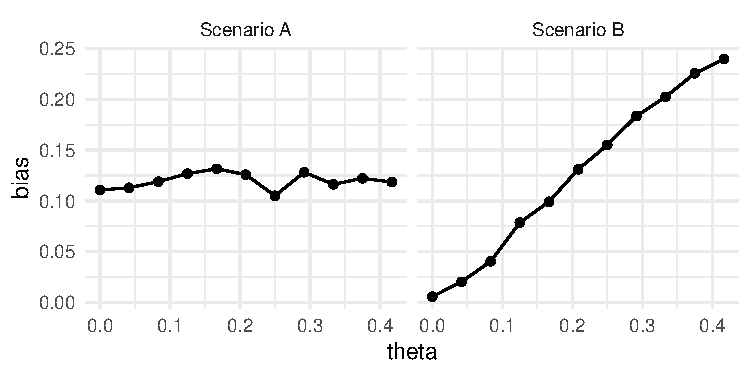
\includegraphics[width=0.75\linewidth]{Designing-Simulations-in-R_files/figure-latex/unnamed-chunk-102-1} \end{center}

If the absolute bias is roughly the same for all values of \(\theta\) (as in Scenario A), then it makes sense to report absolute bias as the summary performance criterion.
On the other hand, if the bias grows roughly in proportion to \(\theta\) (as in Scenario B), then relative bias might be a better summary criterion.

\textbf{Performance relative to a baseline estimator.}

Another relative measure, as we saw earlier, is to calculate performance relative to some baseline.
For example, if one of the estimators is the ``generic method,'' we could calculate ratios of the RMSE of our estimators to the baseline RMSE.
This can provide a way of standardizing across simulation scenarios where the overall scale of the RMSE changes radically.
This could be critical to, for example, examining trends across simulations that have different sample sizes, where we would expect all estimators' performance measures to improve as sample size grows.
This kind of relative standardization allows us to make statements such as ``Aggregation has standard errors around 8\% smaller than linear regression''--which is very interpretable, more interpretable than saying ``Aggregation has standard errors around 0.01 smaller than linear regression.''
In the latter case, we do not know if that is big or small.

While a powerful tool, standardization is not without risks: if you scale relative to something, then higher or lower ratios can either be due to the primary method of interest (the numerator) or due to the behavior of the reference method in the denominator.
These relative ratios can end up being confusing to interpret due to this tension.

They can also break when everything is on a constrained scale, like power.
If we have a power of 0.05, and we improve it to 0.10, we have doubled our power, but if it is 0.10 and we increase to 0.15, we have only increased by 50\%.
Ratios when near zero can be very deceiving.

\subsection{Robust Measures of Performance}\label{robust-measures-of-performance}

Depending on the model and estimation procedures being examined, a range of different criteria might be used to assess estimator performance.
For point estimation, we have seen bias, variance and MSE as the three core measures of performance.
Other criteria exist, such as the median bias and the median absolute deviation of \(T\), where we use the median \(\tilde{T}\) of our estimates rather than the mean \(\bar{T}\).

The usual bias, variance and MSE measures can be sensitive to outliers.
If an estimator generally does well, except for an occasional large mistake, these classic measures can return very poor overall performance.
Instead, we might turn to quantities such as the median bias (sort all the estimation errors across the simulation scenarios, and take the middle), or the Median Absolute Distance (MAD, where you take the median of the absolute values of the errors, which is an alternative to RMSE) as a measure of performance.

Other robust measures are also possible, such as simply truncating all errors to a maximum size (this is called Windsorizing).
This is a way of saying ``I don't care if you are off by 1000, I am only going to count it as 10.''

\subsection{Summary of Peformance Measures}\label{summary-of-peformance-measures}

We list most of the performance criteria we saw in this chapter in the table below, for reference:

\begin{longtable}[]{@{}
  >{\raggedright\arraybackslash}p{(\columnwidth - 4\tabcolsep) * \real{0.2500}}
  >{\raggedright\arraybackslash}p{(\columnwidth - 4\tabcolsep) * \real{0.3833}}
  >{\raggedright\arraybackslash}p{(\columnwidth - 4\tabcolsep) * \real{0.3667}}@{}}
\toprule\noalign{}
\begin{minipage}[b]{\linewidth}\raggedright
Criterion
\end{minipage} & \begin{minipage}[b]{\linewidth}\raggedright
Definition
\end{minipage} & \begin{minipage}[b]{\linewidth}\raggedright
Estimate
\end{minipage} \\
\midrule\noalign{}
\endhead
\bottomrule\noalign{}
\endlastfoot
Bias & \(\text{E}(T) - \theta\) & \(\bar{T} - \theta\) \\
Median bias & \(\text{M}(T) - \theta\) & \(\tilde{T} - \theta\) \\
Variance & \(\text{E}\left[\left(T - \text{E}(T)\right)^2\right]\) & \(S_T^2\) \\
MSE & \(\text{E}\left[\left(T - \theta\right)^2\right]\) & \(\left(\bar{T} - \theta\right)^2 + S_T^2\) \\
MAD & \(\text{M}\left[\left|T - \theta\right|\right]\) & \(\left[\left|T - \theta\right|\right]_{R/2}\) \\
Relative bias & \(\text{E}(T) / \theta\) & \(\bar{T} / \theta\) \\
Relative median bias & \(\text{M}(T) / \theta\) & \(\tilde{T} / \theta\) \\
Relative MSE & \(\text{E}\left[\left(T - \theta\right)^2\right] / \theta^2\) & \(\frac{\left(\bar{T} - \theta\right)^2 + S_T^2}{\theta^2}\) \\
\end{longtable}

\begin{itemize}
\tightlist
\item
  Bias and median bias are measures of whether the estimator is systematically higher or lower than the target parameter.
\item
  Variance is a measure of the \textbf{precision} of the estimator---that is, how far it deviates \emph{from its average}. We might look at the square root of this, to assess the precision in the units of the original measure. This is the true SE of the estimator.
\item
  Mean-squared error is a measure of \textbf{overall accuracy}, i.e.~is a measure how far we typically are from the truth. We more frequently use the root mean-squared error, or RMSE, which is just the square root of the MSE.
\item
  The median absolute deviation (MAD) is another measure of overall accuracy that is less sensitive to outlier estimates. The RMSE can be driven up by a single bad egg. The MAD is less sensitive to this.
\end{itemize}

\section{Uncertainty in Performance Estimates (the MCSE)}\label{uncertainty-in-performance-estimates-the-mcse}

Our performance criteria are defined as average performance across an infinite number of trials.
Of course, in our simulations we only run a finite number of trials, and estimate the performance criteria with the sample of trials we generate.
For example, if we are assessing coverage across 100 trials, we can calculate what fraction rejected the null for that 100.
This is an \emph{estimate} of the true coverage rate.
Due to random chance, we might see a higher, or lower, proportion rejected than what we would see if we ran the simulation forever.

To account for estimation uncertainty we want associated uncertainty estimates to go with our point estimates of performance.
We want to, in other words, treat our simulation results as a dataset in its own right.
(And yes, this is quite meta!)

Once we frame the problem in these terms, it is relatively straightforward to calculate standard errors for most of the performance critera because we have an independent and identically distributed set of measurements.
We call these standard errors Monte Carlo Simulation Errors, or MCSEs.
For some of the performance criteria we have to be a bit more clever, as we will discuss below.

We list MCSE expressions for many of our straightforward performance measures on the following table.
In reading the table, recall that, for an estimator \(T\), we have \(S_T\) being the standard deviation of \(T\) across our simulation runs (i.e., our estimated true Standard Error).
We also have

\begin{itemize}
\tightlist
\item
  Sample skewness (standardized): \(\displaystyle{g_T = \frac{1}{R S_T^3}\sum_{r=1}^R \left(T_r - \bar{T}\right)^3}\)
\item
  Sample kurtosis (standardized): \(\displaystyle{k_T = \frac{1}{R S_T^4} \sum_{r=1}^R \left(T_r - \bar{T}\right)^4}\)
\end{itemize}

\begin{longtable}[]{@{}
  >{\raggedright\arraybackslash}p{(\columnwidth - 2\tabcolsep) * \real{0.6667}}
  >{\raggedright\arraybackslash}p{(\columnwidth - 2\tabcolsep) * \real{0.3333}}@{}}
\toprule\noalign{}
\begin{minipage}[b]{\linewidth}\raggedright
Criterion for T
\end{minipage} & \begin{minipage}[b]{\linewidth}\raggedright
MCSE
\end{minipage} \\
\midrule\noalign{}
\endhead
\bottomrule\noalign{}
\endlastfoot
Bias (\(T-\theta\)) & \(\sqrt{S_T^2/ R}\) \\
Variance (\(S_T^2\)) & \(\displaystyle{S_T^2 \sqrt{\frac{k_T - 1}{R}}}\) \\
MSE & see below \\
MAD & - \\
Power \& Validity (\(r_\alpha\)) & \(\sqrt{ r_\alpha \left(1 - r_\alpha\right) / R}\) \\
Coverage (\(\omega_\beta\)) & \(\sqrt{\omega_\beta \left(1 - \omega_\beta\right) / R}\) \\
Average length (\(\text{E}(W)\)) & \(\sqrt{S_W^2 / R}\) \\
\end{longtable}

The MCSE for the MSE is a bit more complicated, and does not quite fit on our table:
\[ \widehat{MCSE}( \widehat{MSE} ) = \displaystyle{\sqrt{\frac{1}{R}\left[S_T^4 (k_T - 1) + 4 S_T^3 g_T\left(\bar{T} - \theta\right) + 4 S_T^2 \left(\bar{T} - \theta\right)^2\right]}} .\]

For relative quantities with respect to an estimand, simply divide the criterion by the target estimand.
E.g., for relative bias \(T / \theta\), the standard error would be
\[ SE\left( \frac{T}{\theta} \right) = \frac{1}{\theta} SE(T) = \sqrt{\frac{S_T^2}{R\theta^2}} .\]

For square rooted quantities, such as the SE for the true SE (square root of the Variance) or the RMSE (square root of MSE) we can use the Delta method.
The Delta method says (with some conditions), that if we assume \(X \sim N( \phi, V )\), then we can approximate the distribution of \(g(X)\) for some continuous function \(g(\cdot)\) as
\[ g(X) \sim N\left( g(\phi), \;\; g'(\phi)^2\cdot V \right) , \]
where \(g'(\phi)\) is the derivative of \(g(\cdot)\) evaluated at \(\phi\).
In other words,
\[ SE( g(\hat{X}) ) \approx g'(\theta)  \times SE(\hat{X}) .\]
For estimation, we plug in \(\hat{\theta}\) and our estimate of \(SE(\hat{X})\) into the above.
Back to the square root, we have \(g(x) = \sqrt(x)\) and \(g'(x) = 1/2\sqrt(x)\).
This gives, for example, the estimated MCSE of the SE as
\[ \widehat{SE}( \widehat{SE} ) = \widehat{SE}( S^2_T ) = \frac{1}{2S^2_T} \widehat{SE}( S^2_T ) = \frac{1}{2S^2_T} S_T^2 \sqrt{\frac{k_T - 1}{R}} = \frac{1}{2} \sqrt{\frac{k_T - 1}{R}} .\]

\subsection{MCSE for Relative Variance Estimators}\label{mcse-for-relative-variance-estimators}

Estimating the MCSE of the relative bias or relative MSE of a (squared) standard error estimator, i.e., of \(E( \widehat{SE^2} - SE^2 ) / SE^2 )\) or \(\widehat{MSE} / MSE\), is complicated by the appearance of an estimated quantity, \(SE^2\) or \(MSE\), in the denominator of the ratio.
This renders the simple division approach from above unusable, technically speaking.
The problem is we cannot use our clean expressions for MCSEs of relative performance measures since we are not taking the uncertainty of our denominator into account.

To properly assess the overall MCSE, we need to do something else.
One approach is to use the \emph{jackknife} technique.
Let \(\bar{V}_{(j)}\) and \(S_{T(j)}^2\) be the average squared standard error estimate and the true variance estimate calculated from the set of replicates \textbf{\emph{that excludes replicate \(j\)}}, for \(j = 1,...,R\).
The relative bias estimate, excluding replicate \(j\) would then be \(\bar{V}_{(j)} / S_{T(j)}^2\).
Calculating all \(R\) versions of this relative bias estimate and taking the variance of these \(R\) versions yields the jackknife variance estimator:

\[
MCSE\left( \frac{ \widehat{SE}^2 }{SE^2} \right) = \frac{1}{R} \sum_{j=1}^R \left(\frac{\bar{V}_{(j)}}{S_{T(j)}^2} - \frac{\bar{V}}{S_T^2}\right)^2.
\]

This would be quite time-consuming to compute if we did it by brute force. However, a few algebra tricks provide a much quicker way. The tricks come from observing that

\[
\begin{aligned}
\bar{V}_{(j)} &= \frac{1}{R - 1}\left(R \bar{V} - V_j\right) \\
S_{T(j)}^2 &= \frac{1}{R - 2} \left[(R - 1) S_T^2 - \frac{R}{R - 1}\left(T_j - \bar{T}\right)^2\right]
\end{aligned}
\]
These formulas can be used to avoid re-computing the mean and sample variance from every subsample.
Instead, you calculate the overall mean and overall variance, and then do a small adjustment with each jackknife iteration.
You can even implement this with vector processing in R!

\subsection{\texorpdfstring{Calculating MCSEs With the \texttt{simhelpers} Package}{Calculating MCSEs With the simhelpers Package}}\label{calculating-mcses-with-the-simhelpers-package}

The \texttt{simhelper} package is designed to calculate MCSEs (and the performance metrics themselves) for you.
It is easy to use: take this set of simulation runs on the Welch dataset:

\begin{Shaded}
\begin{Highlighting}[]
\FunctionTok{library}\NormalTok{( simhelpers )}
\FunctionTok{data}\NormalTok{( welch\_res )}
\NormalTok{welch }\OtherTok{\textless{}{-}}\NormalTok{ welch\_res }\SpecialCharTok{\%\textgreater{}\%}
  \FunctionTok{filter}\NormalTok{( method }\SpecialCharTok{==} \StringTok{"t{-}test"}\NormalTok{ ) }\SpecialCharTok{\%\textgreater{}\%}
\NormalTok{  dplyr}\SpecialCharTok{::}\FunctionTok{select}\NormalTok{( }\SpecialCharTok{{-}}\NormalTok{method, }\SpecialCharTok{{-}}\NormalTok{seed, }\SpecialCharTok{{-}}\NormalTok{iterations )}

\NormalTok{welch}
\end{Highlighting}
\end{Shaded}

\begin{verbatim}
## # A tibble: 8,000 x 8
##       n1    n2 mean_diff      est    var p_val
##    <dbl> <dbl>     <dbl>    <dbl>  <dbl> <dbl>
##  1    50    50         0  0.0258  0.0954 0.934
##  2    50    50         0  0.00516 0.0848 0.986
##  3    50    50         0 -0.0798  0.0818 0.781
##  4    50    50         0 -0.0589  0.102  0.854
##  5    50    50         0  0.0251  0.118  0.942
##  6    50    50         0 -0.115   0.106  0.725
##  7    50    50         0  0.157   0.115  0.645
##  8    50    50         0 -0.213   0.121  0.543
##  9    50    50         0  0.509   0.117  0.139
## 10    50    50         0 -0.354   0.0774 0.206
## # i 7,990 more rows
## # i 2 more variables: lower_bound <dbl>,
## #   upper_bound <dbl>
\end{verbatim}

We can calculate performance metrics across all the range of scenarios.
Here is the rejection rate:

\begin{Shaded}
\begin{Highlighting}[]
\NormalTok{welch\_sub }\OtherTok{=} \FunctionTok{filter}\NormalTok{( welch, n1 }\SpecialCharTok{==} \DecValTok{50}\NormalTok{, n2 }\SpecialCharTok{==} \DecValTok{50}\NormalTok{, mean\_diff}\SpecialCharTok{==}\DecValTok{0}\NormalTok{ )}
\FunctionTok{calc\_rejection}\NormalTok{(welch\_sub, p\_val)}
\end{Highlighting}
\end{Shaded}

\begin{verbatim}
##   K_rejection rej_rate rej_rate_mcse
## 1        1000    0.048   0.006759882
\end{verbatim}

And coverage:

\begin{Shaded}
\begin{Highlighting}[]
\FunctionTok{calc\_coverage}\NormalTok{(welch\_sub, lower\_bound, upper\_bound, mean\_diff)}
\end{Highlighting}
\end{Shaded}

\begin{verbatim}
## # A tibble: 1 x 5
##   K_coverage coverage coverage_mcse width
##        <int>    <dbl>         <dbl> <dbl>
## 1       1000    0.952       0.00676  1.25
## # i 1 more variable: width_mcse <dbl>
\end{verbatim}

Using \texttt{tidyverse} it is easy to process across scenarios (more on experimental design and multiple scenarios later):

\begin{Shaded}
\begin{Highlighting}[]
\NormalTok{welch }\SpecialCharTok{\%\textgreater{}\%} \FunctionTok{group\_by}\NormalTok{(n1,n2,mean\_diff) }\SpecialCharTok{\%\textgreater{}\%}
  \FunctionTok{summarise}\NormalTok{( }\FunctionTok{calc\_rejection}\NormalTok{( }\AttributeTok{p\_values =}\NormalTok{ p\_val ) )}
\end{Highlighting}
\end{Shaded}

\begin{verbatim}
## # A tibble: 8 x 6
## # Groups:   n1, n2 [2]
##      n1    n2 mean_diff K_rejection rej_rate
##   <dbl> <dbl>     <dbl>       <int>    <dbl>
## 1    50    50       0          1000    0.048
## 2    50    50       0.5        1000    0.34 
## 3    50    50       1          1000    0.876
## 4    50    50       2          1000    1    
## 5    50    70       0          1000    0.027
## 6    50    70       0.5        1000    0.341
## 7    50    70       1          1000    0.904
## 8    50    70       2          1000    1    
## # i 1 more variable: rej_rate_mcse <dbl>
\end{verbatim}

\subsection{MCSE Calculation in our Cluster RCT Example}\label{mcse-calculation-in-our-cluster-rct-example}

We can check our MCSEs for our performance measures to see if we have enough simulation trials to give us precise enough estimates to believe the differences we reported earlier.
In particular, we have:

\begin{Shaded}
\begin{Highlighting}[]
\FunctionTok{library}\NormalTok{( simhelpers )}
\NormalTok{runs}\SpecialCharTok{$}\NormalTok{ATE }\OtherTok{=}\NormalTok{ ATE}
\NormalTok{runs }\SpecialCharTok{\%\textgreater{}\%} 
  \FunctionTok{summarise}\NormalTok{( }\FunctionTok{calc\_absolute}\NormalTok{( }\AttributeTok{estimates =}\NormalTok{ ATE\_hat,}
                            \AttributeTok{true\_param =}\NormalTok{ ATE,}
                            \AttributeTok{criteria =} \FunctionTok{c}\NormalTok{(}\StringTok{"bias"}\NormalTok{,}\StringTok{"stddev"}\NormalTok{, }\StringTok{"rmse"}\NormalTok{)) ) }\SpecialCharTok{\%\textgreater{}\%}
\NormalTok{  dplyr}\SpecialCharTok{::}\FunctionTok{select}\NormalTok{( }\SpecialCharTok{{-}}\NormalTok{K\_absolute ) }\SpecialCharTok{\%\textgreater{}\%}
\NormalTok{  knitr}\SpecialCharTok{::}\FunctionTok{kable}\NormalTok{(}\AttributeTok{digits=}\DecValTok{3}\NormalTok{)}
\end{Highlighting}
\end{Shaded}

\begin{tabular}{r|r|r|r|r|r}
\hline
bias & bias\_mcse & stddev & stddev\_mcse & rmse & rmse\_mcse\\
\hline
0.034 & 0.003 & 0.178 & 0.002 & 0.181 & 0.003\\
\hline
\end{tabular}

We see the MCSEs are quite small relative to the linear regression bias term and all the SEs (\texttt{stddev}) and RMSEs: we have simulated enough runs to see the gross trends identified.
We have \emph{not} simulated enough to for sure know if MLM and Agg are not slightly biased. Given our MCSEs, they could have true bias of around 0.01 (two MCSEs).

\section{Exercises}\label{exercises-4}

\begin{enumerate}
\def\labelenumi{\arabic{enumi}.}
\item
  Continuing the exercises from the prior chapters, estimate rejection rates of the BFF* test for the parameter values in the fifth line of Table 1 of Brown and Forsythe (1974).
\item
  Implement the jackknife as described above in code. Check your answers against the \texttt{simhelpers} package for the built-in \texttt{t\_res} dataset:
\end{enumerate}

\begin{Shaded}
\begin{Highlighting}[]
\FunctionTok{library}\NormalTok{( simhelpers )}
\FunctionTok{calc\_relative}\NormalTok{(}\AttributeTok{data =}\NormalTok{ t\_res, }\AttributeTok{estimates =}\NormalTok{ est, }\AttributeTok{true\_param =}\NormalTok{ true\_param)}
\end{Highlighting}
\end{Shaded}

\begin{verbatim}
## # A tibble: 1 x 7
##   K_relative rel_bias rel_bias_mcse rel_mse
##        <int>    <dbl>         <dbl>   <dbl>
## 1       1000     1.00        0.0128   0.163
## # i 3 more variables: rel_mse_mcse <dbl>,
## #   rel_rmse <dbl>, rel_rmse_mcse <dbl>
\end{verbatim}

\begin{enumerate}
\def\labelenumi{\arabic{enumi}.}
\setcounter{enumi}{2}
\tightlist
\item
  As foreground to the following chapters, can you explore multiple scenarios for the cluster RCT example to see if the trends are common? First write a function that takes a parameter, runs the entire simulation, and returns the results as a small table. You pick which parameter, e.g., average treatment effect, \texttt{alpha}, or whatever you like), that you wish to vary. Here is a skeleton for the function:
\end{enumerate}

\begin{Shaded}
\begin{Highlighting}[]
\NormalTok{my\_simulation }\OtherTok{\textless{}{-}} \ControlFlowTok{function}\NormalTok{( my\_param ) \{}
  \CommentTok{\# call the sim\_function() simulation function from the end of last}
  \CommentTok{\# chapter, setting the parameter you want to vary to my\_param}
  
  \CommentTok{\# Analyze the results, generating a table of performance metrics,}
  \CommentTok{\# e.g., bias or coverage. Make sure your analysis is a data frame,}
  \CommentTok{\# like we saw earlier this chapter.}
  
  \CommentTok{\# Return results}
\NormalTok{\}}
\end{Highlighting}
\end{Shaded}

Then use code like the following to generate a set of results measured as a function of a varying parameter:

\begin{Shaded}
\begin{Highlighting}[]
\NormalTok{vals }\OtherTok{=} \FunctionTok{seq}\NormalTok{( start, stop, }\AttributeTok{length.out =} \DecValTok{5}\NormalTok{ )}
\NormalTok{res }\OtherTok{=} \FunctionTok{map\_df}\NormalTok{( vals, my\_simulation ) }
\end{Highlighting}
\end{Shaded}

The above code will give you a data frame of results, one column for each performance measure.
Finally, you can use this table and plot the performance measure as a function of the varying parameter.

\chapter{Project: Cronbach Alpha}\label{case_Cronbach}

In this section we walk through a case study of Cronbach Alpha to give an extended ``project,'' or series of exercises, that illustrate writing a complete simulation generated by the filling out of the code skeleton we get from \texttt{simhelpers}'s \texttt{create\_skeleton()} package.

\section{Background}\label{background}

Cronbach's \(\alpha\) coefficient is commonly reported as a measure of the internal consistency among a set of test items. Consider a set of \(p\) test items with population variance-covariance matrix \(\boldsymbol\Phi = \left[\phi_{ij}\right]_{i,j=1}^p\), where \(\phi_{ij}\) is the covariance of item \(i\) and item \(j\) on the test, across all students taking the test.
This population variance-covariance matrix describes how our \(p\) test items co-vary.

Cronback's \(\alpha\) is, under this model, defined as
\[
\alpha = \frac{p}{p - 1}\left(1 - \frac{\sum_{i=1}^p \phi_{ii}}{\sum_{i=1}^p \sum_{j=1}^p \phi_{ij}}\right).
\]

Given a sample of size \(n\), the usual estimate of \(\alpha\) is obtained by replacing the population variances and covariances with corresponding sample estimates. Letting \(s_{ij}\) denote the sample covariance of items \(i\) and \(j\)

\[
A = \frac{p}{p - 1}\left(1 - \frac{\sum_{i=1}^p s_{ii}}{\sum_{i=1}^p \sum_{j=1}^p s_{ij}}\right).
\]

If we assume that the items follow a multivariate normal distribution, then \(A\) corresponds to the maximum likelihood estimator of \(\alpha\).

Our goal is to examine the properties of \(A\) when the set of \(P\) items is \emph{not} multi-variate normal, but rather follows a multivariate \(t\) distribution with \(v\) degrees of freedom.
For simplicity, we shall assume that the items have common variance and have a \textbf{compound symmetric} covariance matrix, such that \(\phi_{11} = \phi_{22} = \cdots = \phi_{pp} = \phi\) and \(\phi_{ij} = \rho \phi\). In this case we can simplify our expression for \(\alpha\) to

\[
\alpha = \frac{p \rho}{1 + \rho (p - 1)}.
\]

\section{Getting started}\label{getting-started}

First create the skeleton of our simulation.
We will then walk through filling in all the pieces.

\begin{Shaded}
\begin{Highlighting}[]
\FunctionTok{library}\NormalTok{( simhelpers )}
\FunctionTok{create\_skeleton}\NormalTok{()}
\end{Highlighting}
\end{Shaded}

\section{The data-generating function}\label{the-data-generating-function}

The first two sections in the skeleton are about the data-generating model:

\begin{Shaded}
\begin{Highlighting}[]
\FunctionTok{rm}\NormalTok{(}\AttributeTok{list =} \FunctionTok{ls}\NormalTok{())}

\CommentTok{\#{-}{-}{-}{-}{-}{-}{-}{-}{-}{-}{-}{-}{-}{-}{-}{-}{-}{-}{-}{-}{-}{-}{-}{-}{-}{-}{-}{-}{-}{-}{-}{-}{-}{-}{-}{-}{-}{-}{-}{-}{-}{-}{-}{-}{-}{-}{-}{-}{-}{-}{-}{-}{-}{-}}
\CommentTok{\# Set development values for simulation parameters}
\CommentTok{\#{-}{-}{-}{-}{-}{-}{-}{-}{-}{-}{-}{-}{-}{-}{-}{-}{-}{-}{-}{-}{-}{-}{-}{-}{-}{-}{-}{-}{-}{-}{-}{-}{-}{-}{-}{-}{-}{-}{-}{-}{-}{-}{-}{-}{-}{-}{-}{-}{-}{-}{-}{-}{-}{-}}

\CommentTok{\# What are your model parameters?}
\CommentTok{\# What are your design parameters?}

\CommentTok{\#{-}{-}{-}{-}{-}{-}{-}{-}{-}{-}{-}{-}{-}{-}{-}{-}{-}{-}{-}{-}{-}{-}{-}{-}{-}{-}{-}{-}{-}{-}{-}{-}{-}{-}{-}{-}{-}{-}{-}{-}{-}{-}{-}{-}{-}{-}{-}{-}{-}{-}{-}{-}{-}{-}}
\CommentTok{\# Data Generating Model}
\CommentTok{\#{-}{-}{-}{-}{-}{-}{-}{-}{-}{-}{-}{-}{-}{-}{-}{-}{-}{-}{-}{-}{-}{-}{-}{-}{-}{-}{-}{-}{-}{-}{-}{-}{-}{-}{-}{-}{-}{-}{-}{-}{-}{-}{-}{-}{-}{-}{-}{-}{-}{-}{-}{-}{-}{-}}

\NormalTok{dgm }\OtherTok{\textless{}{-}} \ControlFlowTok{function}\NormalTok{(model\_params) \{}

  \FunctionTok{return}\NormalTok{(dat)}
\NormalTok{\}}

\CommentTok{\# Test the data{-}generating model {-} How can you verify that it is correct?}
\end{Highlighting}
\end{Shaded}

We need to create and test a function that takes model parameters (and sample sizes and such) as inputs, and produces a simulated dataset.
The following function generates a sample of \(n\) observations of \(p\) items from a multivariate \(t\)-distribution with a compound symmetric covariance matrix, intra-class correlation \(\rho\), and \(v\) degrees of freedom:

\begin{Shaded}
\begin{Highlighting}[]
\CommentTok{\# model parameters}
\NormalTok{alpha }\OtherTok{\textless{}{-}} \FloatTok{0.73} \CommentTok{\# true alpha}
\NormalTok{df }\OtherTok{\textless{}{-}} \DecValTok{12} \CommentTok{\# degrees of freedom}

\CommentTok{\# design parameters}
\NormalTok{n }\OtherTok{\textless{}{-}} \DecValTok{50} \CommentTok{\# sample size}
\NormalTok{p }\OtherTok{\textless{}{-}} \DecValTok{6} \CommentTok{\# number of items}


\FunctionTok{library}\NormalTok{(mvtnorm)}

\NormalTok{r\_mvt\_items }\OtherTok{\textless{}{-}} \ControlFlowTok{function}\NormalTok{(n, p, alpha, df) \{}
\NormalTok{  icc }\OtherTok{\textless{}{-}}\NormalTok{ alpha }\SpecialCharTok{/}\NormalTok{ (p }\SpecialCharTok{{-}}\NormalTok{ alpha }\SpecialCharTok{*}\NormalTok{ (p }\SpecialCharTok{{-}} \DecValTok{1}\NormalTok{))}
\NormalTok{  V\_mat }\OtherTok{\textless{}{-}}\NormalTok{ icc }\SpecialCharTok{+} \FunctionTok{diag}\NormalTok{(}\DecValTok{1} \SpecialCharTok{{-}}\NormalTok{ icc, }\AttributeTok{nrow =}\NormalTok{ p)}
\NormalTok{  X }\OtherTok{\textless{}{-}} \FunctionTok{rmvt}\NormalTok{(}\AttributeTok{n =}\NormalTok{ n, }\AttributeTok{sigma =}\NormalTok{ V\_mat, }\AttributeTok{df =}\NormalTok{ df)}
  \FunctionTok{colnames}\NormalTok{(X) }\OtherTok{\textless{}{-}}\NormalTok{ LETTERS[}\DecValTok{1}\SpecialCharTok{:}\NormalTok{p]}
\NormalTok{  X}
\NormalTok{\}}
\end{Highlighting}
\end{Shaded}

Note how we translate the target \(\alpha\) to \(ICC\) for our DGP; we will see this type of translation more later on.

We check our method first to see if we get the right kind of data:

\begin{Shaded}
\begin{Highlighting}[]
\NormalTok{small\_sample }\OtherTok{\textless{}{-}} \FunctionTok{r\_mvt\_items}\NormalTok{(}\AttributeTok{n =} \DecValTok{8}\NormalTok{, }\AttributeTok{p =} \DecValTok{3}\NormalTok{, }\AttributeTok{alpha =} \FloatTok{0.73}\NormalTok{, }\AttributeTok{df =} \DecValTok{5}\NormalTok{)}
\NormalTok{small\_sample}
\end{Highlighting}
\end{Shaded}

\begin{verbatim}
##               A          B           C
## [1,]  2.3124033  1.4871021  0.31446430
## [2,] -1.4587950 -1.3283014  0.63908069
## [3,]  1.5629021 -0.8914364 -0.54087633
## [4,] -0.3940601 -0.5341222  0.67531815
## [5,]  0.3540992  1.0526006  0.30111128
## [6,] -0.6923360 -2.4674208 -0.83354515
## [7,]  1.0175186  1.3437649  1.02493679
## [8,] -0.7536926 -0.8084425 -0.09497557
\end{verbatim}

It looks like we have 8 observations of 3 items, as desired.

To check that the function is indeed simulating data following the intended distribution, let's next generate a very large sample of items. We can then verify that the correlation matrix of the items is compound-symmetric and that the marginal distributions of the items follow \(t\)-distributions with specified degrees of freedom.

\begin{Shaded}
\begin{Highlighting}[]
\NormalTok{big\_sample }\OtherTok{\textless{}{-}} \FunctionTok{r\_mvt\_items}\NormalTok{(}\AttributeTok{n =} \DecValTok{100000}\NormalTok{, }\AttributeTok{p =} \DecValTok{4}\NormalTok{, }\AttributeTok{alpha =} \FloatTok{0.73}\NormalTok{, }\AttributeTok{df =} \DecValTok{5}\NormalTok{)}
\FunctionTok{round}\NormalTok{(}\FunctionTok{cor}\NormalTok{(big\_sample), }\DecValTok{3}\NormalTok{)}
\end{Highlighting}
\end{Shaded}

\begin{verbatim}
##       A     B     C     D
## A 1.000 0.398 0.395 0.396
## B 0.398 1.000 0.393 0.400
## C 0.395 0.393 1.000 0.402
## D 0.396 0.400 0.402 1.000
\end{verbatim}

Is this what it should look like?

We can also check normality:

\begin{Shaded}
\begin{Highlighting}[]
\FunctionTok{qqplot}\NormalTok{(}\FunctionTok{qt}\NormalTok{(}\FunctionTok{ppoints}\NormalTok{(}\DecValTok{200}\NormalTok{), }\AttributeTok{df =} \DecValTok{5}\NormalTok{), big\_sample[,}\DecValTok{2}\NormalTok{], }\AttributeTok{ylim =} \FunctionTok{c}\NormalTok{(}\SpecialCharTok{{-}}\DecValTok{4}\NormalTok{,}\DecValTok{4}\NormalTok{))}
\end{Highlighting}
\end{Shaded}

\begin{center}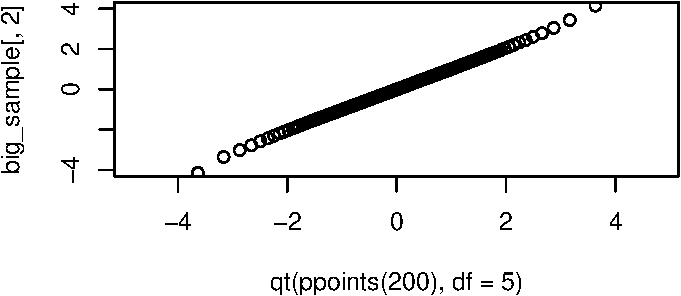
\includegraphics[width=0.75\linewidth]{Designing-Simulations-in-R_files/figure-latex/unnamed-chunk-116-1} \end{center}

Looks good! A nice straight line.

\section{The estimation function}\label{the-estimation-function}

The next section of the template looks like this:

\begin{Shaded}
\begin{Highlighting}[]
\CommentTok{\#{-}{-}{-}{-}{-}{-}{-}{-}{-}{-}{-}{-}{-}{-}{-}{-}{-}{-}{-}{-}{-}{-}{-}{-}{-}{-}{-}{-}{-}{-}{-}{-}{-}{-}{-}{-}{-}{-}{-}{-}{-}{-}{-}{-}{-}{-}{-}{-}{-}{-}{-}{-}{-}{-}}
\CommentTok{\# Model{-}fitting/estimation/testing functions}
\CommentTok{\#{-}{-}{-}{-}{-}{-}{-}{-}{-}{-}{-}{-}{-}{-}{-}{-}{-}{-}{-}{-}{-}{-}{-}{-}{-}{-}{-}{-}{-}{-}{-}{-}{-}{-}{-}{-}{-}{-}{-}{-}{-}{-}{-}{-}{-}{-}{-}{-}{-}{-}{-}{-}{-}{-}}

\NormalTok{estimate }\OtherTok{\textless{}{-}} \ControlFlowTok{function}\NormalTok{(dat, design\_params) \{}

  \FunctionTok{return}\NormalTok{(result)}
\NormalTok{\}}

\CommentTok{\# Test the estimation function}
\end{Highlighting}
\end{Shaded}

van Zyl, Neudecker, and Nel (2000) demonstrate that, if the items have a compound-symmetric covariance matrix, then the asymptotic variance of \(A\) is
\[
\text{Var}(A) \approx \frac{2p(1 - \alpha)^2}{(p - 1) n}.
\]
Substituting \(A\) in place of \(\alpha\) on the right hand side gives an estimate of the variance of \(A\). The following function calculates \(A\) and its variance estimator from a sample of data:

\begin{Shaded}
\begin{Highlighting}[]
\NormalTok{estimate\_alpha }\OtherTok{\textless{}{-}} \ControlFlowTok{function}\NormalTok{(dat) \{}
\NormalTok{  V }\OtherTok{\textless{}{-}} \FunctionTok{cov}\NormalTok{(dat)}
\NormalTok{  p }\OtherTok{\textless{}{-}} \FunctionTok{ncol}\NormalTok{(dat)}
\NormalTok{  n }\OtherTok{\textless{}{-}} \FunctionTok{nrow}\NormalTok{(dat)}
  
  \CommentTok{\# Calculate A with our formula}
\NormalTok{  A }\OtherTok{\textless{}{-}}\NormalTok{ p }\SpecialCharTok{/}\NormalTok{ (p }\SpecialCharTok{{-}} \DecValTok{1}\NormalTok{) }\SpecialCharTok{*}\NormalTok{ (}\DecValTok{1} \SpecialCharTok{{-}} \FunctionTok{sum}\NormalTok{(}\FunctionTok{diag}\NormalTok{(V)) }\SpecialCharTok{/} \FunctionTok{sum}\NormalTok{(V))}
  
  \CommentTok{\# Calculate our estimate of the variance (SE\^{}2) of A}
\NormalTok{  Var\_A }\OtherTok{\textless{}{-}} \DecValTok{2} \SpecialCharTok{*}\NormalTok{ p }\SpecialCharTok{*}\NormalTok{ (}\DecValTok{1} \SpecialCharTok{{-}}\NormalTok{ A)}\SpecialCharTok{\^{}}\DecValTok{2} \SpecialCharTok{/}\NormalTok{ ((p }\SpecialCharTok{{-}} \DecValTok{1}\NormalTok{) }\SpecialCharTok{*}\NormalTok{ n)}
  
  \CommentTok{\# Pack up our results}
  \FunctionTok{data.frame}\NormalTok{(}\AttributeTok{A =}\NormalTok{ A, }\AttributeTok{Var =}\NormalTok{ Var\_A)}
\NormalTok{\}}

\FunctionTok{estimate\_alpha}\NormalTok{(small\_sample)}
\end{Highlighting}
\end{Shaded}

\begin{verbatim}
##           A        Var
## 1 0.7080628 0.03196024
\end{verbatim}

The \texttt{psych} package provides a function for calculating \(\alpha\), which can be used to verify that the calculation of \(A\) in \texttt{estimate\_alpha} is correct:

\begin{Shaded}
\begin{Highlighting}[]
\FunctionTok{library}\NormalTok{(psych)}
\FunctionTok{summary}\NormalTok{(}\FunctionTok{alpha}\NormalTok{(}\AttributeTok{x =}\NormalTok{ small\_sample))}\SpecialCharTok{$}\NormalTok{raw\_alpha}
\end{Highlighting}
\end{Shaded}

\begin{verbatim}
## Number of categories should be increased  in order to count frequencies.
\end{verbatim}

\begin{verbatim}
## 
## Reliability analysis   
##  raw_alpha std.alpha G6(smc) average_r S/N  ase
##       0.71       0.7    0.87      0.44 2.4 0.13
##   mean   sd median_r
##  0.054 0.93     0.63
\end{verbatim}

\begin{verbatim}
## NULL
\end{verbatim}

The next step is to evaluate these individual estimates and see how well our estimator \(A\) performs.

\subsection{Exercices (Naive confidence intervals)}\label{exercices-naive-confidence-intervals}

\begin{enumerate}
\def\labelenumi{\arabic{enumi}.}
\tightlist
\item
  One way to obtain an approximate confidence interval for \(\alpha\) would be to take \(A \pm z \sqrt{\text{Var}(A)}\), where \(\text{Var}(A)\) is estimated as described above and \(z\) is a standard normal critical value at the appropriate level (i.e., \(z = 1.96\) for a 95\% CI).
  Extend your simulation to calculate a confidence interval for each simulation round (put this code inside \texttt{estimate\_alpha()}) and then calculate confidence interval coverage.
\end{enumerate}

Your \texttt{estimate\_alpha} would then give a result like this:

\begin{Shaded}
\begin{Highlighting}[]
\FunctionTok{set.seed}\NormalTok{(}\DecValTok{40200}\NormalTok{)}
\NormalTok{dat }\OtherTok{=} \FunctionTok{r\_mvt\_items}\NormalTok{(}\AttributeTok{n =} \DecValTok{50}\NormalTok{, }\AttributeTok{p =} \DecValTok{5}\NormalTok{, }\AttributeTok{alpha =} \FloatTok{0.9}\NormalTok{, }\AttributeTok{df =} \DecValTok{3}\NormalTok{ )}
\FunctionTok{estimate\_alpha}\NormalTok{(dat)}
\end{Highlighting}
\end{Shaded}

\begin{verbatim}
##           A          Var   CI_low   CI_high
## 1 0.9425904 0.0001647933 0.916916 0.9682647
\end{verbatim}

\begin{enumerate}
\def\labelenumi{\arabic{enumi}.}
\setcounter{enumi}{1}
\tightlist
\item
  You can calculate confidence intervals with coverage other than 95\% by calculating an appropriate number of standard errors, \(z\) (usually just taken as 2, as above, for a nominal 95\%), with
\end{enumerate}

\begin{Shaded}
\begin{Highlighting}[]
\NormalTok{coverage }\OtherTok{=} \FloatTok{0.95}
\NormalTok{z }\OtherTok{=} \FunctionTok{qnorm}\NormalTok{( (}\DecValTok{1}\SpecialCharTok{{-}}\NormalTok{coverage) }\SpecialCharTok{/} \DecValTok{2}\NormalTok{, }\AttributeTok{lower.tail =} \ConstantTok{FALSE}\NormalTok{ )}
\NormalTok{z}
\end{Highlighting}
\end{Shaded}

\begin{verbatim}
## [1] 1.959964
\end{verbatim}

Extend \texttt{estimate\_alpha()} to allow for a specified coverage by adding a parameter, \texttt{coverage}, along with a default of 0.95. Revise the body of \texttt{estimate\_alpha} to calculate a confidence interval with the specified coverage rate.

\section{Estimator performance}\label{estimator-performance}

The next section of the template deals with performance calculations.

\begin{Shaded}
\begin{Highlighting}[]
\CommentTok{\#{-}{-}{-}{-}{-}{-}{-}{-}{-}{-}{-}{-}{-}{-}{-}{-}{-}{-}{-}{-}{-}{-}{-}{-}{-}{-}{-}{-}{-}{-}{-}{-}{-}{-}{-}{-}{-}{-}{-}{-}{-}{-}{-}{-}{-}{-}{-}{-}{-}{-}{-}{-}{-}{-}}
\CommentTok{\# Calculate performance measures}
\CommentTok{\# (For some simulations, it may make more sense}
\CommentTok{\# to do this as part of the simulation driver.)}
\CommentTok{\#{-}{-}{-}{-}{-}{-}{-}{-}{-}{-}{-}{-}{-}{-}{-}{-}{-}{-}{-}{-}{-}{-}{-}{-}{-}{-}{-}{-}{-}{-}{-}{-}{-}{-}{-}{-}{-}{-}{-}{-}{-}{-}{-}{-}{-}{-}{-}{-}{-}{-}{-}{-}{-}{-}}

\NormalTok{performance }\OtherTok{\textless{}{-}} \ControlFlowTok{function}\NormalTok{(results, model\_params) \{}

  \FunctionTok{return}\NormalTok{(performance\_measures)}
\NormalTok{\}}

\CommentTok{\# Check performance calculations}
\end{Highlighting}
\end{Shaded}

The \texttt{performance()} function takes as input a bunch of simulated data (which we might call \texttt{results}) and the true values of the model parameters (\texttt{model\_params}) and returns as output a set of summary performance measures. As noted in the comments above, for simple simulations it might not be necessary to write a separate function to do these calculations. For more complex simulations, though, it can be helpful to break these calculations out in a function.

To start to get the code working that we would put into this function, it is useful to start with some simulation replicates to practice on.
We can generate 1000 replicates using samples of size \(n = 40\), \(p = 6\) items, a true \(\alpha = 0.8\), and \(v = 5\) degrees of freedom:

\begin{Shaded}
\begin{Highlighting}[]
\NormalTok{one\_run }\OtherTok{\textless{}{-}} \ControlFlowTok{function}\NormalTok{( n, p, alpha, df ) \{}
\NormalTok{    dat }\OtherTok{\textless{}{-}} \FunctionTok{r\_mvt\_items}\NormalTok{(}\AttributeTok{n =}\NormalTok{ n, }\AttributeTok{p =}\NormalTok{ p, }\AttributeTok{alpha =}\NormalTok{ alpha, }\AttributeTok{df =}\NormalTok{ df)}
    \FunctionTok{estimate\_alpha}\NormalTok{(dat)}
\NormalTok{\}}
\NormalTok{true\_alpha }\OtherTok{=} \FloatTok{0.7}
\NormalTok{results }\OtherTok{=} \FunctionTok{rerun}\NormalTok{( }\DecValTok{1000}\NormalTok{, }\FunctionTok{one\_run}\NormalTok{(}\DecValTok{40}\NormalTok{, }\DecValTok{6}\NormalTok{, }\AttributeTok{alpha=}\NormalTok{true\_alpha, }\AttributeTok{df=}\DecValTok{5}\NormalTok{) ) }\SpecialCharTok{\%\textgreater{}\%}
  \FunctionTok{bind\_rows}\NormalTok{()}
\end{Highlighting}
\end{Shaded}

\begin{verbatim}
## Warning: `rerun()` was deprecated in purrr 1.0.0.
## i Please use `map()` instead.
##   # Previously
## rerun(1000, one_run(40, 6, alpha = true_alpha,
## df = 5))
## 
##   # Now
## map(1:1000, ~ one_run(40, 6, alpha = true_alpha,
## df = 5))
## This warning is displayed once every 8 hours.
## Call `lifecycle::last_lifecycle_warnings()` to
## see where this warning was generated.
\end{verbatim}

\subsection{Exercises (Calculating Performance)}\label{exercises-calculating-performance}

For the Cronbach alpha simulation, we might want to calculate the following performance measures:

\begin{enumerate}
\def\labelenumi{\arabic{enumi}.}
\item
  With the parameters specified above, calculate the bias of \(A\). Also calculate the Monte Carlo standard error (MCSE) of the bias estimate.
\item
  Estimate the true Standard Error of \(A\).
\item
  Calculate the mean squared error of \(A\).
\item
  Calculate the relative bias of the asymptotic variance estimator.
\item
  Using the work from above, wrap your code in an \texttt{alpha\_performance()} function that takes the results of uses \texttt{run\_alpha\_sim} and returns a one-row data frame with columns corresponding to the bias, mean squared error, relative bias of the asymptotic variance estimator.
\end{enumerate}

E.g.,

\begin{Shaded}
\begin{Highlighting}[]
\FunctionTok{alpha\_performance}\NormalTok{(results, true\_alpha)}
\end{Highlighting}
\end{Shaded}

\begin{verbatim}
##          bias     bias_SE        SE       MSE
## 1 -0.02329445 0.003741931 0.1183302 0.1205433
##    bias_Var
## 1 0.5078144
\end{verbatim}

\begin{enumerate}
\def\labelenumi{\arabic{enumi}.}
\setcounter{enumi}{5}
\item
  Extend your function to add in the MCSEs for the SE and MSE. Code up the skewness and kurtosis values by hand, using the formula in the MCSE section of the performance measure chapter.
\item
  \textbf{(Challenge problem)} Code up a jackknife MCSE function to calculate the MCSE for the relative bias of the asymptotic variance estimator.
  Use the following template that takes a vector of point estimates and associated standard errors.
\end{enumerate}

\begin{Shaded}
\begin{Highlighting}[]
\NormalTok{jackknife\_MCSE }\OtherTok{\textless{}{-}} \ControlFlowTok{function}\NormalTok{( estimates, SEs ) \{}
  \CommentTok{\# code}
\NormalTok{\}}
\end{Highlighting}
\end{Shaded}

You would use this function as:

\begin{Shaded}
\begin{Highlighting}[]
\FunctionTok{jackknife\_MCSE}\NormalTok{( alpha\_reps}\SpecialCharTok{$}\NormalTok{A, }\FunctionTok{sqrt}\NormalTok{( alpha\_reps}\SpecialCharTok{$}\NormalTok{Var ) )}
\end{Highlighting}
\end{Shaded}

\section{Replication (and the simulation)}\label{replication-and-the-simulation}

We now have all the components we need to get simulation results, given a set of parameter values.
In the next section of the template, we put all these pieces together in a function---which we might call the \emph{simulation driver}---that takes as input 1) parameter values, 2) the desired number of replications, and 3) optionally, a seed value (this allows for reproducability, see Chapter \ref{sec-reproducability}. The function produces as output a single set of performance estimates. Generically, the function looks like this:

\begin{Shaded}
\begin{Highlighting}[]
\CommentTok{\#{-}{-}{-}{-}{-}{-}{-}{-}{-}{-}{-}{-}{-}{-}{-}{-}{-}{-}{-}{-}{-}{-}{-}{-}{-}{-}{-}{-}{-}{-}{-}{-}{-}{-}{-}{-}{-}{-}{-}{-}{-}{-}{-}{-}{-}{-}{-}{-}{-}{-}{-}{-}{-}{-}{-}{-}{-}{-}{-}}
\CommentTok{\# Simulation Driver {-} should return a data.frame or tibble}
\CommentTok{\#{-}{-}{-}{-}{-}{-}{-}{-}{-}{-}{-}{-}{-}{-}{-}{-}{-}{-}{-}{-}{-}{-}{-}{-}{-}{-}{-}{-}{-}{-}{-}{-}{-}{-}{-}{-}{-}{-}{-}{-}{-}{-}{-}{-}{-}{-}{-}{-}{-}{-}{-}{-}{-}{-}{-}{-}{-}{-}{-}}

\NormalTok{runSim }\OtherTok{\textless{}{-}} \ControlFlowTok{function}\NormalTok{(iterations, model\_params, design\_params, }\AttributeTok{seed =} \ConstantTok{NULL}\NormalTok{) \{}
  \ControlFlowTok{if}\NormalTok{ (}\SpecialCharTok{!}\FunctionTok{is.null}\NormalTok{(seed)) }\FunctionTok{set.seed}\NormalTok{(seed)}

\NormalTok{  results }\OtherTok{\textless{}{-}} \FunctionTok{rerun}\NormalTok{(iterations, \{}
\NormalTok{                dat }\OtherTok{\textless{}{-}} \FunctionTok{dgm}\NormalTok{(model\_params)}
                \FunctionTok{estimate}\NormalTok{(dat, design\_params)}
\NormalTok{              \}) }\SpecialCharTok{\%\textgreater{}\%}
    \FunctionTok{bind\_rows}\NormalTok{()}
  

  \FunctionTok{performance}\NormalTok{(results, model\_params)}
\NormalTok{\}}

\CommentTok{\# demonstrate the simulation driver}
\end{Highlighting}
\end{Shaded}

The \texttt{runSim} function should require very little modification for a new simulation. Essentially, all we need to change is the names of the functions that are called, so that they line up with the functions we have designed for our simulation. Here's what this looks like for the Cronbach alpha simulation (we pull out the code to replicate into its own method, \texttt{one\_run()}, which helps with debugging):

\begin{Shaded}
\begin{Highlighting}[]
\CommentTok{\#{-}{-}{-}{-}{-}{-}{-}{-}{-}{-}{-}{-}{-}{-}{-}{-}{-}{-}{-}{-}{-}{-}{-}{-}{-}{-}{-}{-}{-}{-}{-}{-}{-}{-}{-}{-}{-}{-}{-}{-}{-}{-}{-}{-}{-}{-}{-}{-}{-}{-}{-}{-}{-}{-}{-}{-}{-}{-}{-}}
\CommentTok{\# Simulation Driver {-} should return a data.frame or tibble}
\CommentTok{\#{-}{-}{-}{-}{-}{-}{-}{-}{-}{-}{-}{-}{-}{-}{-}{-}{-}{-}{-}{-}{-}{-}{-}{-}{-}{-}{-}{-}{-}{-}{-}{-}{-}{-}{-}{-}{-}{-}{-}{-}{-}{-}{-}{-}{-}{-}{-}{-}{-}{-}{-}{-}{-}{-}{-}{-}{-}{-}{-}}


\NormalTok{one\_run }\OtherTok{\textless{}{-}} \ControlFlowTok{function}\NormalTok{( n, p, alpha, df ) \{}
\NormalTok{    dat }\OtherTok{\textless{}{-}} \FunctionTok{r\_mvt\_items}\NormalTok{(}\AttributeTok{n =}\NormalTok{ n, }\AttributeTok{p =}\NormalTok{ p, }\AttributeTok{alpha =}\NormalTok{ alpha, }\AttributeTok{df =}\NormalTok{ df)}
    \FunctionTok{estimate\_alpha}\NormalTok{(dat)}
\NormalTok{\}}


\NormalTok{run\_alpha\_sim }\OtherTok{\textless{}{-}} \ControlFlowTok{function}\NormalTok{(iterations, n, p, alpha, df, }\AttributeTok{seed =} \ConstantTok{NULL}\NormalTok{) \{}
  
  \ControlFlowTok{if}\NormalTok{ (}\SpecialCharTok{!}\FunctionTok{is.null}\NormalTok{(seed)) }\FunctionTok{set.seed}\NormalTok{(seed)}

\NormalTok{  results }\OtherTok{\textless{}{-}} 
    \FunctionTok{rerun}\NormalTok{(iterations, }\FunctionTok{one\_run}\NormalTok{(n, p, alpha, df) ) }\SpecialCharTok{\%\textgreater{}\%}
    \FunctionTok{bind\_rows}\NormalTok{()}
  
  \FunctionTok{alpha\_performance}\NormalTok{(results, }\AttributeTok{alpha =}\NormalTok{ alpha)}
\NormalTok{\}}
\end{Highlighting}
\end{Shaded}

\section{Extension: Confidence interval coverage}\label{extension-confidence-interval-coverage}

However, van Zyl, Neudecker, and Nel (2000) suggest that a better approximation involves first applying a transformation to \(A\) (to make it more normal in shape), then calculating a confidence interval, then back-transforming to the original scale (this is very similar to the procedure for calculating confidence intervals for correlation coefficients, using Fisher's \(z\) transformation). Let our transformed parameter and estimator be

\[
\begin{aligned}
\beta &= \frac{1}{2} \ln\left(1 - \alpha\right) \\
B &= \frac{1}{2} \ln\left(1 - A\right)
\end{aligned}
\]

and our transformed variance estimator be

\[
V^B = \frac{p}{2 n (p - 1)}.
\]
(This expression comes from a Delta method expansion on \(A\).)

An approximate confidence interval for \(\beta\) is given by \([B_L, B_U]\), where

\[
B_L = B - z \sqrt{V^B}, \qquad B_U = B + z \sqrt{V^B}.
\]

Applying the inverse of the transformation gives a confidence interval for \(\alpha\):

\[
\left[1 - \exp(2B_U), \ 1 - \exp(2 B_L)\right].
\]

\section{A taste of multiple scenarios}\label{a-taste-of-multiple-scenarios}

In the previous sections, we've created code that will generate a set of performance estimates, given a set of parameter values. We can created a dataset that represents every combination of parameter values that we want to examine. How do we put the pieces together?

If we only had a couple of parameter combinations, it would be easy enough to just call our \texttt{run\_alpha\_sim} function a couple of times:

\begin{Shaded}
\begin{Highlighting}[]
\FunctionTok{run\_alpha\_sim}\NormalTok{(}\AttributeTok{iterations =} \DecValTok{100}\NormalTok{, }\AttributeTok{n =} \DecValTok{50}\NormalTok{, }\AttributeTok{p =} \DecValTok{4}\NormalTok{, }\AttributeTok{alpha =} \FloatTok{0.7}\NormalTok{, }\AttributeTok{df =} \DecValTok{5}\NormalTok{)}
\end{Highlighting}
\end{Shaded}

\begin{verbatim}
## Warning: `rerun()` was deprecated in purrr 1.0.0.
## i Please use `map()` instead.
##   # Previously
##   rerun(100, one_run(n, p, alpha, df))
## 
##   # Now
##   map(1:100, ~ one_run(n, p, alpha, df))
## This warning is displayed once every 8 hours.
## Call `lifecycle::last_lifecycle_warnings()` to
## see where this warning was generated.
\end{verbatim}

\begin{verbatim}
##          bias    bias_SE        SE       MSE
## 1 -0.01211522 0.01088426 0.1088426 0.1089725
##    bias_Var
## 1 0.4913622
\end{verbatim}

\begin{Shaded}
\begin{Highlighting}[]
\FunctionTok{run\_alpha\_sim}\NormalTok{(}\AttributeTok{iterations =} \DecValTok{100}\NormalTok{, }\AttributeTok{n =} \DecValTok{100}\NormalTok{, }\AttributeTok{p =} \DecValTok{4}\NormalTok{, }\AttributeTok{alpha =} \FloatTok{0.7}\NormalTok{, }\AttributeTok{df =} \DecValTok{5}\NormalTok{)}
\end{Highlighting}
\end{Shaded}

\begin{verbatim}
##         bias    bias_SE        SE        MSE
## 1 -0.0117337 0.00761985 0.0761985 0.07671916
##    bias_Var
## 1 0.4727169
\end{verbatim}

\begin{Shaded}
\begin{Highlighting}[]
\FunctionTok{run\_alpha\_sim}\NormalTok{(}\AttributeTok{iterations =} \DecValTok{100}\NormalTok{, }\AttributeTok{n =} \DecValTok{50}\NormalTok{, }\AttributeTok{p =} \DecValTok{8}\NormalTok{, }\AttributeTok{alpha =} \FloatTok{0.7}\NormalTok{, }\AttributeTok{df =} \DecValTok{5}\NormalTok{)}
\end{Highlighting}
\end{Shaded}

\begin{verbatim}
##          bias    bias_SE        SE       MSE
## 1 -0.02601087 0.01120983 0.1120983 0.1145292
##    bias_Var
## 1 0.4319068
\end{verbatim}

\begin{Shaded}
\begin{Highlighting}[]
\FunctionTok{run\_alpha\_sim}\NormalTok{(}\AttributeTok{iterations =} \DecValTok{100}\NormalTok{, }\AttributeTok{n =} \DecValTok{100}\NormalTok{, }\AttributeTok{p =} \DecValTok{8}\NormalTok{, }\AttributeTok{alpha =} \FloatTok{0.7}\NormalTok{, }\AttributeTok{df =} \DecValTok{5}\NormalTok{)}
\end{Highlighting}
\end{Shaded}

\begin{verbatim}
##          bias     bias_SE         SE        MSE
## 1 0.007758062 0.006203414 0.06203414 0.06220884
##    bias_Var
## 1 0.5299059
\end{verbatim}

But in an actual simulation we will probably have too many different combinations to do this ``by hand.''
The final sections of the simulation template demonstrate two different approaches to doing the calculations for \emph{every} combination of parameter values, given a set of parameter values one wants to explore.

This is discussed further in Chapter @ref(exp\_design), but let's get a small taste of doing this now.
In particular, the following code will evaluate the performance of \(A\) for true values of \(\alpha\) ranging from 0.5 to 0.9 (i.e., \texttt{alpha\_true\_seq\ \textless{}-\ seq(0.5,\ 0.9,\ 0.1)}) via \texttt{map\_df()}:

\begin{Shaded}
\begin{Highlighting}[]
\NormalTok{alpha\_true\_seq }\OtherTok{\textless{}{-}} \FunctionTok{seq}\NormalTok{(}\FloatTok{0.5}\NormalTok{, }\FloatTok{0.9}\NormalTok{, }\FloatTok{0.1}\NormalTok{)}
\NormalTok{results }\OtherTok{\textless{}{-}} \FunctionTok{map\_df}\NormalTok{( alpha\_true\_seq, }
\NormalTok{                   run\_simulation,}
                   \AttributeTok{R =} \DecValTok{100}\NormalTok{,}
                   \AttributeTok{n =} \DecValTok{50}\NormalTok{, }\AttributeTok{p =} \DecValTok{5}\NormalTok{, }\AttributeTok{df =} \DecValTok{5}\NormalTok{ )}
\end{Highlighting}
\end{Shaded}

How does coverage change for different values of \(A\)?

\subsection{Exercises}\label{exercises-5}

\begin{enumerate}
\def\labelenumi{\arabic{enumi}.}
\item
  Show the inverse transform of \(B = g(A)\) gives the above expression.
\item
  Make a new function, \texttt{estimate\_alpha\_xform()} that, given a dataset, calculates a confidence interval for \(\alpha\) following the method described above.
\item
  Using the modified \texttt{estimate\_alpha\_xform()}, generate 1000 replicated confidence intervals for \(n = 40\), \(p = 6\) items, a true \(\alpha = 0.8\), and \(v = 5\) degrees of freedom. Using these replicates, calculate the true coverage rate of the confidence interval. Also calculate the Monte Carlo standard error (MCSE) of this coverage rate.
\item
  Calculate the average length of the confidence interval for \(\alpha\), along with its MCSE.
\item
  Compare the results of this approach to the more naive approach. Are there gains in performance?
\item
  \emph{Challenge} Derive the variance expression for the transformed estimator using the Delta method on the variance expression for \(A\) coupled with the transform. The Delta method says that:
\end{enumerate}

\[ var( f(A) ) \approx \frac{1}{f'(\alpha)} (A - \alpha)^2 . \]

\chapter{Case study: Attrition in a simple randomized experiment}\label{case-study-attrition-in-a-simple-randomized-experiment}

Missingness of the outcome variable is a common problem in randomized experiments conducted with human participants. For experiments where the focus is on estimating average causal effects, many different strategies for handling attrition have been proposed. Gerber and Green (2012) describe several strategies, including:

\begin{itemize}
\tightlist
\item
  Complete-case analysis, in which observations with missing outcome data are simply dropped from analysis;
\item
  Regression estimation under the assumption that missingness is independent of potential outcomes, conditional on a set of pre-treatment covariates; and
\item
  Monotone treatment response bounds, which provides bounds on the average treatment effect among participants who would provide outcome data under any treatment condition, under the assumption that that the effect of treatment on providing outcome data is strictly non-negative.
\end{itemize}

In this case study, we will develop a data-generating process that allows us to study these different estimation strategies. To make things interesting, we will examine a scenario in which the data include covariates that influence the probability of providing outcome data under treatment and under control, as well as being predictive of the outcome.

To formalize these notions, let us define the following variables:

\begin{itemize}
\tightlist
\item
  \(X\): a continuous covariate
\item
  \(C\): a binary covariate
\item
  \(A\): an indicator for whether a participant provides outcome data if assigned to treatment (latent)
\item
  \(R\): an indicator for whether a participant provides outcome data if assigned to control, given that \(A = 1\) (latent)
\item
  \(Z\): a randomized treatment indicator
\item
  \(Y^0, Y^1\): potential outcomes (latent)
\item
  \(Y^F\): the outcome that would be observed if all participants were to respond (latent)
\item
  \(Y\): the measured outcome, which is only observed for some participants
\item
  \(O\): an indicator for whether the outcome \(Y\) is observed
\end{itemize}

We will posit that these variables are related as follows:

\textbf{TODO / NOTE: Dag code broken -- need to fix}

Now, let's lay out a more specific distributional model:
\[
\begin{aligned}
X &\sim N(0,1) \\
C &\sim Bern(\kappa) - \kappa\\
Z &\sim Bern(0.5) \\
A &\sim Bern\left(\pi_A(C,X)\right) \\
R &\sim Bern\left(\pi_R(C,X)\right)
\end{aligned}
\]
where the response indicators follow the models
\[
\begin{aligned}
\text{logit} \ \pi_A(C,X) &= \alpha_{A0} + \alpha_{A1} C + \alpha_{A2} X \\
\text{logit} \ \pi_R(C,X) &= \alpha_{R0} + \alpha_{R1} C + \alpha_{R2} X.
\end{aligned}
\]
Next, let \(B\) denote \(\text{E}(Y^0 | A, R, C, X)\) and suppose that
\[
B = \beta_0 + \beta_1 C + \beta_2 X + \beta_3 R + \beta_4 C \times R + \beta_5 X \times R.
\]
Let \(D\) denote the the treatment effect surface, \(\text{E}(Y^1 - Y^0 | A, R, C, X)\), and suppose that
\[
D = \delta_0 + \delta_1 C + \delta_2 X + \delta_3 R + \delta_4 C \times R + \delta_5 X \times R.
\]
Note that these models do not differentiate between the never-responders (who have \(A = 0\)) and those who respond only if assigned to treatment (who have \(A = 1, R = 0\)) because the outcome will never be observed for never-responders.

With these functions, we define the potential outcomes as
\[
\begin{aligned}
Y^0 &= B + e_0 \\
Y^1 &= B + D + e_1,
\end{aligned}
\]
where \((e_0, e_1)\) are bivariate normal with means of zero, standard deviations \(\sigma_0, \sigma_1\), and correlation \(\rho\).

The remaining variables in the model are structurally related to those previously defined:
\[
\begin{aligned}
O &= (1 - Z) R A + Z A \\
Y^F &= (1 - Z) Y^0 + Z Y^1 \\
Y &= \begin{cases} Y^F & \text{if} \quad O = 1 \\ 
\cdot & \text{if} \quad O = 0. \end{cases}
\end{aligned}
\]
The observed data include the variables \(X, C, Z, O\), and \(Y\).

\section{The data generating process}\label{the-data-generating-process}

Let's write a function to generate data based on this model. Here's a skeleton to get started:

\begin{Shaded}
\begin{Highlighting}[]
\NormalTok{sim\_attrition\_data }\OtherTok{\textless{}{-}} \ControlFlowTok{function}\NormalTok{(}
\NormalTok{    N,                      }\CommentTok{\# sample size}
\NormalTok{    kappa,                  }\CommentTok{\# probability of C}
\NormalTok{    alpha\_A,                }\CommentTok{\# regression for response under treatment}
\NormalTok{    alpha\_R,                }\CommentTok{\# regression for response under control}
\NormalTok{    beta,                   }\CommentTok{\# regression parameters for Y0}
\NormalTok{    delta,                  }\CommentTok{\# regression parameters for treatment response}
    \AttributeTok{sigma0 =} \DecValTok{1}\NormalTok{, }\AttributeTok{sigma1 =} \DecValTok{1}\NormalTok{, }\CommentTok{\# conditional standard deviation of potential outcomes}
\NormalTok{    rho                     }\CommentTok{\# conditional correlation between potential outcomes}
\NormalTok{) \{}
  \CommentTok{\# generate data frame}
  \FunctionTok{return}\NormalTok{(df)}
\NormalTok{\}}
\end{Highlighting}
\end{Shaded}

\section{Estimators}\label{estimators}

What estimators might we use with these data?

\section{Performance criteria}\label{performance-criteria-1}

What performance criteria should we look at?

\part{Multifactor Simulations}\label{part-multifactor-simulations}

\chapter{Designing the multifactor simulation experiment}\label{exp-design}

So far, we've created code that will give us results for a single combination of parameter values.
In practice, simulation studies typically examine a range of different values, including varying the level of the true parameter values and perhaps also varying sample sizes, to explore a range of different scenarios.
We either want reassurance that our findings are general, or we want to understand what aspects of the context lead to our found results.
A single simulation gives us no hint as to either of these questions.
It is only by looking across a range of settings that we can fully understand trade-offs, general rules, and limits.
Let's now look at the remaining piece of the simulation puzzle: the study's experimental design.

Simulation studies often take the form of \textbf{full factorial} designed experiments. In full factorials, each factor (a particular knob a researcher might turn to change the simulation conditions) is varied across multiple levels, and the design includes \emph{every} possible combination of the levels of every factor. One way to represent such a design is as a list of factors and levels.

For example, for the Cronbach alpha simulation, we might want to vary:

\begin{itemize}
\tightlist
\item
  the sample size, with values of 50 or 100; and
\item
  the number of items, with values of 4 or 8.
\item
  the true value of alpha, with values ranging from 0.1 to 0.9;
\item
  the degrees of freedom of the multivariate \(t\) distribution, with values of 5, 10, 20, or 100;
\end{itemize}

We first express the simulation parameters as a list of factors, each factor having a list of values to explore.
We will then run a simulation for every possible combination of these values.
We call this a \(2 \times 2 \times 9 \times 4\) factorial design, where each element is the number of options for that factor.
Here is code that generates all the scenarios we will run given the above design, storing these combinations in a data frame, \texttt{params}, that represents the full experimental design:

\begin{Shaded}
\begin{Highlighting}[]
\NormalTok{design\_factors }\OtherTok{\textless{}{-}} \FunctionTok{list}\NormalTok{(}
  \AttributeTok{n =} \FunctionTok{c}\NormalTok{(}\DecValTok{50}\NormalTok{, }\DecValTok{100}\NormalTok{),}
  \AttributeTok{p =} \FunctionTok{c}\NormalTok{(}\DecValTok{4}\NormalTok{, }\DecValTok{8}\NormalTok{),}
  \AttributeTok{alpha =} \FunctionTok{seq}\NormalTok{(}\FloatTok{0.1}\NormalTok{, }\FloatTok{0.9}\NormalTok{, }\FloatTok{0.1}\NormalTok{),}
  \AttributeTok{df =} \FunctionTok{c}\NormalTok{(}\DecValTok{5}\NormalTok{, }\DecValTok{10}\NormalTok{, }\DecValTok{20}\NormalTok{, }\DecValTok{100}\NormalTok{)}
\NormalTok{)}

\NormalTok{params }\OtherTok{\textless{}{-}} \FunctionTok{cross\_df}\NormalTok{(design\_factors)}
\NormalTok{params}
\end{Highlighting}
\end{Shaded}

\begin{verbatim}
## # A tibble: 144 x 4
##        n     p alpha    df
##    <dbl> <dbl> <dbl> <dbl>
##  1    50     4   0.1     5
##  2   100     4   0.1     5
##  3    50     8   0.1     5
##  4   100     8   0.1     5
##  5    50     4   0.2     5
##  6   100     4   0.2     5
##  7    50     8   0.2     5
##  8   100     8   0.2     5
##  9    50     4   0.3     5
## 10   100     4   0.3     5
## # i 134 more rows
\end{verbatim}

See what we get?
The parameters we would pass to \texttt{run.experiment()} correspond to the
columns of our dataset.
We have a total of \(2 \times 2 \times 9 \times 4 = 144\) rows, each row corresponding to a simulation scenario to explore.
With multifactor experiments, it is easy to end up running a lot of experiments!

\section{Choosing parameter combinations}\label{choosing-parameter-combinations}

How do we go about choosing parameter values to examine?
Choosing which parameters to use is a central part of good simulation design because the primary limitation of simulation studies is always their \emph{generalizability}.
On the one hand, it's difficult to extrapolate findings from a simulation study beyond the set of simulation conditions that were examined. On the other hand, it's often difficult or impossible to examine the full space of all possible parameter values, except for very simple problems. Even in the Cronbach alpha simulation, we've got four factors, and the last three could each take an infinite number of different levels, in theory. How can we come up with a defensible set of levels to examine?

The choice of simulation conditions needs to be made in the context of the problem or model that you're studying, so it's a bit difficult to offer valid, decontextualized advice.
We can provide a few observations all the same:

\begin{enumerate}
\def\labelenumi{\arabic{enumi}.}
\item
  For research simulations, it often is important to be able to relate your findings to previous research. This suggests that you should select parameter levels to make this possible, such as by looking at sample sizes similar to those examined in previous studies. That said, previous simulation studies are not always perfect (actually, there's a lot of really crummy ones out there!), and so prior work should not geneally be your sole guide or justification.
\item
  Generally, it is better to err on the side of being more comprehensive. You learn more by looking at a broader range of conditions, and you can always boil down your results to a more limited set of conditions for purposes of presentation.
\item
  It is also important to explore breakdown points (e.g., what sample size is too small for a method to work?) rather than focusing only on conditions where a method might be expected to work well. Pushing the boundaries and identifying conditions where estimation methods break will help you to provide better guidance for how the methods should be used in practice.
\end{enumerate}

An important point regarding (2) is that you can be more comprehensive and then have fewer replications per scenario.
For example, say you were planning on doing 1000 simulations per scenario, but then you realize there is some new factor that you don't think matters, but that you believe other researchers will worry about.
You could add in that factor, say with four levels, and then do 250 simulations per scenario.
The total work remains the same.

When analyzing the final simulation you can then first verify you do not see trends along this new factor, and then marganalize out the factor in your summaries of results.
Marginalizing out a factor (i.e., averaging your performance metrics across the additional factor) is a powerful technique of making a claim about how your methods work \emph{on average} across a \emph{range} of scenarios, rather than for a specific scenario.

Overall, you generally want to vary parameters that you believe matter, or that you think other people will believe matter.
The first is so you can learn.
The second is to build your case.

Once you have identified your parameters you then have to decide on the levels of the parameter you will include in the simulation.
There are three strategies you might take:

\begin{enumerate}
\def\labelenumi{\arabic{enumi}.}
\tightlist
\item
  Vary a parameter over its entire range (or nearly so).
\item
  Choose parameter levels to represent realistic practical range.

  \begin{itemize}
  \tightlist
  \item
    Empirical justification based on systematic reviews of applications
  \item
    Or at least informal impressions of what's realistic in practice
  \end{itemize}
\item
  Choose parameters to emulate one important application.
\end{enumerate}

In the above (1) is the most general---but also the most computationally intensive.
(2) will focus attention, ideally, on what is of practical relevance to a practitioner.
(3) is usually coupled with a subsequent applied data analysis, and in this case the simulation is often used to enrich that analysis.
For example, if the simulation shows the methods work for data with the given form of the target application, people may be more willing to believe the application's findings.

Regardless of how you select your primary parameters, you should also vary nuisance parameters (at least a little) to test sensitivity of results.
While simulations will (generally) never be fully generalizable, you can certainly make them so they avoid the obvious things a critic might identify as an easy dismissal of your findings.

To recap, as you think about your parameter selection, always keep the following design principles and acknowledgements:

\begin{itemize}
\tightlist
\item
  The primary limitation of simulation studies is \textbf{generalizability}.
\item
  Choose conditions that allow you to relate findings to previous work.
\item
  Err towards being comprehensive.

  \begin{itemize}
  \tightlist
  \item
    The goal should be to build an understanding of the major moving parts.
  \item
    Presentation of results can always be tailored to illustrate trends.
  \end{itemize}
\item
  Explore breakdown points (e.g., what sample size is too small for applying a given method?).
\end{itemize}

And fully expect to add and subtract from your set of parameters as you get your initial simulation results! No one ever runs just a single simulation.

\subsection{Choosing parameters for the Clustered RCT}\label{choosing-parameters-for-the-clustered-rct}

Extending our case study presented in Section \ref{case-cluster} to a multifactor simulation, let's think about how to design our full experiment.

So far, we have only investigated a single scenario at a time, although our modular approach does make exploring a range of scenarios by re-calling our simulation function relatively straightforward.
But how do our findings generalize? When are the different methods differently appropriate?
To answer this, we need to extend to a multifactor simulation to \emph{systematically} explore trends across contexts for our three estimators.
We begin by identifying some questions we might have, given our preliminary results.

Regarding bias, in our initial simulation, we noticed that Linear Regression is estimating a person-weighted quantity, and so would be considered biased for the site-average ATE.
We might next ask, how much does bias change if we change the site-size by impact relationship?

For precision, we also saw that Linear Regression has a higher standard error.
But is this a general finding? When does this occur?
Are there contexts where linear regression will do better than the others?
Originally we thought aggregation would lose information becuase little sites will have the same weight as big sites, but be more imprecisely estimated.
Were we wrong? Or perhaps if site size was even more variable, Agg might do worse and worse.

Finally, the estimated SEs all appeared to be good, although they were rather variable, relative to the true SE.
We might then ask, is this always the case? Will the estimated SEs fall apart (e.g., be way too large or way too small, in general) in different contexts?

To answer these questions we need to more systematically explore the space of models. But we have a lot of knobs to turn.
In our simulation, we can generate fake cluster randomized data with the following features:

\begin{itemize}
\item
  The treatment impact of the site can vary, and vary with the site size
\item
  We can have sites of different sizes if we want
\item
  We can also vary:

  \begin{itemize}
  \tightlist
  \item
    the site intercept variance
  \item
    the residual variance,
  \item
    the treatment impact
  \item
    the site size
  \item
    the number of sites, \ldots{}
  \end{itemize}
\end{itemize}

We cannot easily vary all of these.
We instead reflect on our research questions, speculate as to what is likely to matter, and then consider varying the following:

\begin{itemize}
\tightlist
\item
  Average site size: Does the number of students/site matter?
\item
  Number of sites: Do cluster-robust SEs work with fewer sites?
\item
  Variation in site size: Varying site sizes cause bias or break things?
\item
  Correlation of site size and site impact: Will correlation cause bias?
\item
  Cross site variation: Does the amount of site variation matter?
\end{itemize}

When designing the final factors, it is important to ensure those factors are isolated, in that changing one of them is not changing a host of other things that might impact performance.
For example, in our case, if we simply added more cross site variation by directly increasing the random effects for the clusters, our total variation will increase.
If we see that methods deteriorate, we then have a confound: is it the cross site variation causing the problem, or is it the total variation?
We therefore want to vary site variation while controlling total variation; this is why we use the ICC knob discussed in the section on the data generation process.

We might thus end up with the following for our factors:

\begin{Shaded}
\begin{Highlighting}[]
\NormalTok{crt\_design\_factors }\OtherTok{\textless{}{-}} \FunctionTok{list}\NormalTok{(}
  \AttributeTok{n\_bar =} \FunctionTok{c}\NormalTok{( }\DecValTok{20}\NormalTok{, }\DecValTok{80}\NormalTok{, }\DecValTok{320}\NormalTok{ ),}
  \AttributeTok{J =} \FunctionTok{c}\NormalTok{( }\DecValTok{5}\NormalTok{, }\DecValTok{20}\NormalTok{, }\DecValTok{80}\NormalTok{ ),}
  \AttributeTok{ATE =} \FunctionTok{c}\NormalTok{( }\FloatTok{0.2}\NormalTok{ ),}
  \AttributeTok{size\_coef =} \FunctionTok{c}\NormalTok{( }\DecValTok{0}\NormalTok{, }\FloatTok{0.2}\NormalTok{ ),}
  \AttributeTok{ICC =} \FunctionTok{c}\NormalTok{( }\DecValTok{0}\NormalTok{, }\FloatTok{0.2}\NormalTok{, }\FloatTok{0.4}\NormalTok{, }\FloatTok{0.6}\NormalTok{, }\FloatTok{0.8}\NormalTok{ ),}
  \AttributeTok{alpha =} \FunctionTok{c}\NormalTok{( }\DecValTok{0}\NormalTok{, }\FloatTok{0.5}\NormalTok{, }\FloatTok{0.8}\NormalTok{ )}
\NormalTok{)}
\end{Highlighting}
\end{Shaded}

\section{Using pmap to run multifactor simulations}\label{using-pmap-to-run-multifactor-simulations}

To run simulations across all of our factor combinations, we are going to use a very useful method in the \texttt{purrr} package called \texttt{pmap()}.
\texttt{pmap()} marches down a set of lists, running a function on each \(p\)-tuple of elements, taking the \(i^{th}\) element from each list for iteration \(i\), and passing them as parameters to the specified function.
\texttt{pmap()} then returns the results of this sequence of function calls as a list of results.

Here is a small illustration:

\begin{Shaded}
\begin{Highlighting}[]
\NormalTok{my\_function }\OtherTok{\textless{}{-}} \ControlFlowTok{function}\NormalTok{( a, b, theta, scale ) \{}
\NormalTok{    scale }\SpecialCharTok{*}\NormalTok{ (a }\SpecialCharTok{+}\NormalTok{ theta}\SpecialCharTok{*}\NormalTok{(b}\SpecialCharTok{{-}}\NormalTok{a))}
\NormalTok{\}}

\NormalTok{args }\OtherTok{=} \FunctionTok{list}\NormalTok{( }\AttributeTok{a =} \DecValTok{1}\SpecialCharTok{:}\DecValTok{3}\NormalTok{, }
             \AttributeTok{b =} \DecValTok{5}\SpecialCharTok{:}\DecValTok{7}\NormalTok{, }
             \AttributeTok{theta =} \FunctionTok{c}\NormalTok{(}\FloatTok{0.2}\NormalTok{, }\FloatTok{0.3}\NormalTok{, }\FloatTok{0.7}\NormalTok{) )}
\NormalTok{purrr}\SpecialCharTok{::}\FunctionTok{pmap\_dbl}\NormalTok{(  args, my\_function, }\AttributeTok{scale =} \DecValTok{10}\NormalTok{ )}
\end{Highlighting}
\end{Shaded}

\begin{verbatim}
## [1] 18 32 58
\end{verbatim}

One important note is the variable names for the lists being iterated over must correspond exactly to function arguments of the called function.
Extra parameters can be passed after the function name; these will be held constant, and passed to each function call.
See how \texttt{scale} is the same for all calls.

As we see above, \texttt{pmap()} has variants such as \texttt{\_dbl} or \texttt{\_df} just like the \texttt{map()} and \texttt{map2()} methods.
These variants will automatically stack or convert the list of things returned into a tidier collection (for \texttt{\_dbl} it will convert to a vector of numbers, for \texttt{\_df} it will stack the results to make a large dataframe, assuming each thing returned is a little dataframe).

So far, this is great, but it does not quite look like what we want: our factors are stored as a dataframe, not three lists.
This is where R gets interesting: in R, the columns of a dataframe are stored as a list of vectors or lists (with each of the vectors or lists having the exact same length).
This works beautifully with \texttt{pmap()}.
Witness:

\begin{Shaded}
\begin{Highlighting}[]
\NormalTok{args[[}\DecValTok{2}\NormalTok{]]}
\end{Highlighting}
\end{Shaded}

\begin{verbatim}
## [1] 5 6 7
\end{verbatim}

\begin{Shaded}
\begin{Highlighting}[]
\NormalTok{a\_df }\OtherTok{=} \FunctionTok{as.data.frame}\NormalTok{(args)}
\NormalTok{a\_df}
\end{Highlighting}
\end{Shaded}

\begin{verbatim}
##   a b theta
## 1 1 5   0.2
## 2 2 6   0.3
## 3 3 7   0.7
\end{verbatim}

\begin{Shaded}
\begin{Highlighting}[]
\NormalTok{a\_df[[}\DecValTok{2}\NormalTok{]]}
\end{Highlighting}
\end{Shaded}

\begin{verbatim}
## [1] 5 6 7
\end{verbatim}

\begin{Shaded}
\begin{Highlighting}[]
\NormalTok{purrr}\SpecialCharTok{::}\FunctionTok{pmap\_dbl}\NormalTok{( a\_df, my\_function, }\AttributeTok{scale =} \DecValTok{10}\NormalTok{)}
\end{Highlighting}
\end{Shaded}

\begin{verbatim}
## [1] 18 32 58
\end{verbatim}

We can pass \texttt{a\_df} to \texttt{pmap}, and \texttt{pmap} takes it as a list of lists, and therefore does exactly what it did before.

All of this means \texttt{pmap()} can run a specified function on each row of a dataset.
Continuing the Cronbach Alpha simulation from above, we would have the following:

\begin{Shaded}
\begin{Highlighting}[]
\NormalTok{params}\SpecialCharTok{$}\NormalTok{iterations }\OtherTok{\textless{}{-}} \DecValTok{500}
\NormalTok{sim\_results }\OtherTok{\textless{}{-}}\NormalTok{  params }\SpecialCharTok{\%\textgreater{}\%}
  \FunctionTok{mutate}\NormalTok{(}\AttributeTok{res =} \FunctionTok{pmap}\NormalTok{(., run\_alpha\_sim ) )}
\end{Highlighting}
\end{Shaded}

We add a column to \texttt{params} to record the desired 500 replications per condition.
The above code calls our \texttt{run\_alpha\_sim()} method for each row of our list of scenarios we want to explore.
Even better, we are storing the results \textbf{as a new variable in the same dataset}.

\begin{Shaded}
\begin{Highlighting}[]
\NormalTok{sim\_results}
\end{Highlighting}
\end{Shaded}

\begin{verbatim}
## # A tibble: 144 x 6
##        n     p alpha    df iterations res  
##    <dbl> <dbl> <dbl> <dbl>      <dbl> <lgl>
##  1    50     4   0.1     5        500 NA   
##  2   100     4   0.1     5        500 NA   
##  3    50     8   0.1     5        500 NA   
##  4   100     8   0.1     5        500 NA   
##  5    50     4   0.2     5        500 NA   
##  6   100     4   0.2     5        500 NA   
##  7    50     8   0.2     5        500 NA   
##  8   100     8   0.2     5        500 NA   
##  9    50     4   0.3     5        500 NA   
## 10   100     4   0.3     5        500 NA   
## # i 134 more rows
\end{verbatim}

We are creating a \textbf{list-column}, where each element in our list column is the little summary of our simulation results for that scenario.
Here is the third scenario, for example:

\begin{Shaded}
\begin{Highlighting}[]
\NormalTok{sim\_results}\SpecialCharTok{$}\NormalTok{res[[}\DecValTok{3}\NormalTok{]]}
\end{Highlighting}
\end{Shaded}

\begin{verbatim}
## [1] NA
\end{verbatim}

We finally use \texttt{unnest()} to expand the \texttt{res} variable, replicating the values of the main variables once for each row in the nested dataset:

\begin{Shaded}
\begin{Highlighting}[]
\FunctionTok{library}\NormalTok{(tidyr)}
\NormalTok{sim\_results }\OtherTok{\textless{}{-}} \FunctionTok{unnest}\NormalTok{(sim\_results, }\AttributeTok{cols =}\NormalTok{ res) }\SpecialCharTok{\%\textgreater{}\%}
\NormalTok{  dplyr}\SpecialCharTok{::}\FunctionTok{select}\NormalTok{( }\SpecialCharTok{{-}}\NormalTok{iterations )}
\NormalTok{sim\_results}
\end{Highlighting}
\end{Shaded}

\begin{verbatim}
## # A tibble: 144 x 5
##        n     p alpha    df res  
##    <dbl> <dbl> <dbl> <dbl> <lgl>
##  1    50     4   0.1     5 NA   
##  2   100     4   0.1     5 NA   
##  3    50     8   0.1     5 NA   
##  4   100     8   0.1     5 NA   
##  5    50     4   0.2     5 NA   
##  6   100     4   0.2     5 NA   
##  7    50     8   0.2     5 NA   
##  8   100     8   0.2     5 NA   
##  9    50     4   0.3     5 NA   
## 10   100     4   0.3     5 NA   
## # i 134 more rows
\end{verbatim}

We can put all of this together in a a tidy workflow as follows:

\begin{Shaded}
\begin{Highlighting}[]
\NormalTok{sim\_results }\OtherTok{\textless{}{-}} 
\NormalTok{  params }\SpecialCharTok{\%\textgreater{}\%}
  \FunctionTok{mutate}\NormalTok{(}\AttributeTok{res =} \FunctionTok{pmap}\NormalTok{(., }\AttributeTok{.f =}\NormalTok{ run\_alpha\_sim)) }\SpecialCharTok{\%\textgreater{}\%}
  \FunctionTok{unnest}\NormalTok{(}\AttributeTok{cols =}\NormalTok{ res)}
\end{Highlighting}
\end{Shaded}

If we wanted to use parallel processing (more on this later) we can also simply use the \texttt{simhelpers} package (the following code is auto-generated by the \texttt{create\_skeleton()} method as well):

\begin{Shaded}
\begin{Highlighting}[]
\FunctionTok{plan}\NormalTok{(multisession) }\CommentTok{\# choose an appropriate plan from the future package}
\FunctionTok{evaluate\_by\_row}\NormalTok{(params, run\_alpha\_sim)}
\end{Highlighting}
\end{Shaded}

We finally save our results using tidyverse's \texttt{write\_csv()}; see ``R for Data Science'' textbook, 11.5.
We can ensure we have a directory by making one via \texttt{dir.create()} (see Section \ref{saving-files} for more on files):

\begin{Shaded}
\begin{Highlighting}[]
\FunctionTok{dir.create}\NormalTok{(}\StringTok{"results"}\NormalTok{, }\AttributeTok{showWarnings =} \ConstantTok{FALSE}\NormalTok{ )}
\FunctionTok{write\_csv}\NormalTok{( sim\_results, }\AttributeTok{file =} \StringTok{"results/cronbach\_results.csv"}\NormalTok{ )}
\end{Highlighting}
\end{Shaded}

\section{Ways of repeating oneself}\label{ways-of-repeating-oneself}

We have three core elements in our simulation:
- Generate data
- Analyze data
- Assess performance

In arranging these elements, we have a choice: do we compute performance measures for each simulation scenario as we go (inside) vs.~computing after we get all of our individual results (outside)?

\emph{INSIDE (aggregate as you simulate):}
In this approach, illustrated above, we, for each scenario defined by a specific combination of factors, run our simulation for that scenario, assess the performance, and then return a nice summary table of how well our methods did.
This is the most straightforward, given what we have done so far: we have a method to run a simulation for a scenario, and we simply run that method for a bunch of scenarios and collate.

After the \texttt{pmap()} call, we end up with a dataframe with all our simulations, one simulation context per row (or maybe bundles, one for each method), with
our measured performance outcomes. This is ideally all we need to analyze.

We have less data to store, and it is easier to compartmentalize.
On the cons side, we have no ability to add new performance measures on the fly.

Overall, this seems pretty good.
That being said, sometimes we might want to use a lot of disk space and keep
much more. In particular, each row of the above corresponds to the summary
of a whole collection of individual runs. We might instead store all of
these runs, which brings us to the other approach.

\emph{OUTSIDE (keep all simulation runs):}
In this approach we do not aggregate, but instead, for each scenario, return the entire set of individual estimates.
The benefit of this is, given the raw estimates, you can dynamically add or change how you calculate performance measures.
You do, however, end up with massive amounts of data to store and manipulate.

To move from inside to outside, we just take the summarizing step out of \texttt{run\_alpha\_sim()}.
E.g.,:

\begin{Shaded}
\begin{Highlighting}[]
\NormalTok{run\_alpha\_sim\_raw }\OtherTok{\textless{}{-}} \ControlFlowTok{function}\NormalTok{(iterations, n, p, alpha, df, }\AttributeTok{coverage =} \FloatTok{0.95}\NormalTok{, }\AttributeTok{seed =} \ConstantTok{NULL}\NormalTok{) \{}
  
  \ControlFlowTok{if}\NormalTok{ (}\SpecialCharTok{!}\FunctionTok{is.null}\NormalTok{(seed)) }\FunctionTok{set.seed}\NormalTok{(seed)}
  
\NormalTok{  results }\OtherTok{\textless{}{-}} 
    \FunctionTok{replicate}\NormalTok{(}\AttributeTok{n =}\NormalTok{ iterations, \{}
\NormalTok{      dat }\OtherTok{\textless{}{-}} \FunctionTok{r\_mvt\_items}\NormalTok{(}\AttributeTok{n =}\NormalTok{ n, }\AttributeTok{p =}\NormalTok{ p, }\AttributeTok{alpha =}\NormalTok{ alpha, }\AttributeTok{df =}\NormalTok{ df)}
      \FunctionTok{estimate\_alpha}\NormalTok{(dat, }\AttributeTok{coverage =}\NormalTok{ coverage)}
\NormalTok{    \}, }\AttributeTok{simplify =} \ConstantTok{FALSE}\NormalTok{) }\SpecialCharTok{\%\textgreater{}\%}
    \FunctionTok{bind\_rows}\NormalTok{()}
  
\NormalTok{  results}
\NormalTok{\}}
\end{Highlighting}
\end{Shaded}

Each call to \texttt{run\_alpha\_sim\_raw()} now gives one row per simulation trial.
We replicate our simulation parameters for each row.

\begin{Shaded}
\begin{Highlighting}[]
\FunctionTok{run\_alpha\_sim\_raw}\NormalTok{( }\DecValTok{4}\NormalTok{, }\DecValTok{50}\NormalTok{, }\DecValTok{6}\NormalTok{, }\FloatTok{0.5}\NormalTok{, }\DecValTok{3}\NormalTok{ )}
\end{Highlighting}
\end{Shaded}

\begin{verbatim}
##           A      Var_A       CI_L      CI_U
## 1 0.5402995 0.01014358 0.29374115 0.7007831
## 2 0.3867717 0.01805035 0.05786946 0.6008526
## 3 0.4617342 0.01390704 0.17303773 0.6496454
## 4 0.4810237 0.01292815 0.20267301 0.6622008
\end{verbatim}

The primary advantage of this is we can then generate new performance measures, as they
occur to us, later on. The disadvantage is this result file will be \(R\)
times as many rows as the older file, which can get quite, quite large.

But disk space is cheap!
Here we run the same experiment with our more
complete storage. Note how the \texttt{pmap\_df} stacks the
multiple rows from each run, giving us everything nicely bundled up:

\begin{Shaded}
\begin{Highlighting}[]
\NormalTok{params}\SpecialCharTok{$}\NormalTok{res }\OtherTok{\textless{}{-}}\NormalTok{ params }\SpecialCharTok{\%\textgreater{}\%} 
    \FunctionTok{pmap}\NormalTok{( run\_alpha\_sim\_raw, }\AttributeTok{iterations =} \DecValTok{500}\NormalTok{ )}
\NormalTok{sim\_results\_full }\OtherTok{\textless{}{-}} \FunctionTok{unnest}\NormalTok{( params,}
                            \AttributeTok{cols =}\NormalTok{ res ) }
\FunctionTok{write\_csv}\NormalTok{( sim\_results\_full, }\StringTok{"results/cronbach\_results\_full.csv"}\NormalTok{ )}
\end{Highlighting}
\end{Shaded}

We end up with a lot more rows:

\begin{Shaded}
\begin{Highlighting}[]
\FunctionTok{nrow}\NormalTok{( sim\_results\_full )}
\end{Highlighting}
\end{Shaded}

\begin{verbatim}
## [1] 72000
\end{verbatim}

\begin{Shaded}
\begin{Highlighting}[]
\FunctionTok{nrow}\NormalTok{( sim\_results )}
\end{Highlighting}
\end{Shaded}

\begin{verbatim}
## [1] 144
\end{verbatim}

Compare the file sizes: one is several k, the other is around 20 megabytes.

\begin{Shaded}
\begin{Highlighting}[]
\FunctionTok{file.size}\NormalTok{(}\StringTok{"results/cronbach\_results.csv"}\NormalTok{) }\SpecialCharTok{/} \DecValTok{1024}
\end{Highlighting}
\end{Shaded}

\begin{verbatim}
## [1] 4.103516
\end{verbatim}

\begin{Shaded}
\begin{Highlighting}[]
\FunctionTok{file.size}\NormalTok{(}\StringTok{"results/cronbach\_results\_full.csv"}\NormalTok{) }\SpecialCharTok{/} \DecValTok{1024}
\end{Highlighting}
\end{Shaded}

\begin{verbatim}
## [1] 7516.222
\end{verbatim}

\subsection{Getting raw results ready for analysis}\label{getting-raw-results-ready-for-analysis}

If we generated raw results then we need to collapse them by experimental run
before calculating performance measures so we can explore the trends across the
experiments.
We do this by grouping our data and calling \texttt{alpha\_performance()} for each group:

\begin{Shaded}
\begin{Highlighting}[]
\NormalTok{results }\OtherTok{\textless{}{-}}\NormalTok{ sim\_results\_full }\SpecialCharTok{\%\textgreater{}\%}
  \FunctionTok{nest\_by}\NormalTok{( n, p, alpha, df, }\AttributeTok{.key =} \StringTok{"alpha\_sims"}\NormalTok{ )}
\NormalTok{results}
\end{Highlighting}
\end{Shaded}

\begin{verbatim}
## # A tibble: 144 x 5
## # Rowwise:  n, p, alpha, df
##        n     p alpha    df         alpha_sims
##    <dbl> <dbl> <dbl> <dbl> <list<tibble[,6]>>
##  1    50     4   0.1     5          [500 x 6]
##  2    50     4   0.1    10          [500 x 6]
##  3    50     4   0.1    20          [500 x 6]
##  4    50     4   0.1   100          [500 x 6]
##  5    50     4   0.2     5          [500 x 6]
##  6    50     4   0.2    10          [500 x 6]
##  7    50     4   0.2    20          [500 x 6]
##  8    50     4   0.2   100          [500 x 6]
##  9    50     4   0.3     5          [500 x 6]
## 10    50     4   0.3    10          [500 x 6]
## # i 134 more rows
\end{verbatim}

\begin{Shaded}
\begin{Highlighting}[]
\NormalTok{results}\SpecialCharTok{$}\NormalTok{performance }\OtherTok{=} \FunctionTok{map2}\NormalTok{( results}\SpecialCharTok{$}\NormalTok{alpha\_sims, }
\NormalTok{                               results}\SpecialCharTok{$}\NormalTok{alpha, alpha\_performance )}
\NormalTok{results }\OtherTok{\textless{}{-}}\NormalTok{ results }\SpecialCharTok{\%\textgreater{}\%}
\NormalTok{  dplyr}\SpecialCharTok{::}\FunctionTok{select}\NormalTok{( }\SpecialCharTok{{-}}\NormalTok{alpha\_sims ) }\SpecialCharTok{\%\textgreater{}\%}
  \FunctionTok{unnest}\NormalTok{( }\AttributeTok{cols=}\StringTok{"performance"}\NormalTok{ ) }
\NormalTok{results}
\end{Highlighting}
\end{Shaded}

\begin{verbatim}
## # A tibble: 576 x 7
## # Groups:   n, p, alpha, df [144]
##        n     p alpha    df criterion           est
##    <dbl> <dbl> <dbl> <dbl> <chr>             <dbl>
##  1    50     4   0.1     5 alpha bias      -0.103 
##  2    50     4   0.1     5 alpha RMSE       0.388 
##  3    50     4   0.1     5 V relative bias  0.436 
##  4    50     4   0.1     5 coverage         0.826 
##  5    50     4   0.1    10 alpha bias      -0.0527
##  6    50     4   0.1    10 alpha RMSE       0.263 
##  7    50     4   0.1    10 V relative bias  0.780 
##  8    50     4   0.1    10 coverage         0.908 
##  9    50     4   0.1    20 alpha bias      -0.0190
## 10    50     4   0.1    20 alpha RMSE       0.221 
## # i 566 more rows
## # i 1 more variable: MCSE <dbl>
\end{verbatim}

\begin{Shaded}
\begin{Highlighting}[]
\CommentTok{\# }\AlertTok{NOTE}\CommentTok{: This is HORRIBLE.  There has to be a better way.}
\end{Highlighting}
\end{Shaded}

Now, if we want to add a performance metric, we can simply change \texttt{alpha\_performance} and recalculate, without running the time-intensive simulations.
Being able to re-analyze your results is generally a far easier fix than running all the simulations again
after changing the \texttt{run\_alpha\_sim()} method.

The results of summarizing during the simulation vs.~after as we just did
leads to essentially the same place, however, although our old results are in long format (with one row per simulation metric vs.~the metrics being columns).

\section{Running the Cluster RCT multifactor experiment}\label{running-the-cluster-rct-multifactor-experiment}

Running our cluster RCT simulation is the exact same code as we have used before.
Simulations take awhile to run so we save them so we can analyze at our leisure.
Because we are not exactly sure what performance metrics we want, we will save our individual results, and calculate performance metrics on the full data.
I.e., we are storing the individual runs, not the analyzed results!

The code is as follows:

\begin{Shaded}
\begin{Highlighting}[]
\NormalTok{params }\OtherTok{\textless{}{-}} 
  \FunctionTok{cross\_df}\NormalTok{(crt\_design\_factors) }\SpecialCharTok{\%\textgreater{}\%}
  \FunctionTok{mutate}\NormalTok{(}
    \AttributeTok{reps =} \DecValTok{100}\NormalTok{,}
    \AttributeTok{seed =} \DecValTok{20200320} \SpecialCharTok{+} \DecValTok{1}\SpecialCharTok{:}\FunctionTok{n}\NormalTok{()}
\NormalTok{  )}
\NormalTok{params}\SpecialCharTok{$}\NormalTok{res }\OtherTok{=} \FunctionTok{pmap}\NormalTok{(params, }\AttributeTok{.f =}\NormalTok{ run\_CRT\_sim )}
\NormalTok{res }\OtherTok{=}\NormalTok{ params }\SpecialCharTok{\%\textgreater{}\%} \FunctionTok{unnest}\NormalTok{( }\AttributeTok{cols=}\FunctionTok{c}\NormalTok{(data) )}
\FunctionTok{saveRDS}\NormalTok{( res, }\AttributeTok{file =} \StringTok{"results/simulation\_CRT.rds"}\NormalTok{ )}
\end{Highlighting}
\end{Shaded}

The seed is for reproducibility; we discuss this more later on.

We then group by our simulation factors and calculate all our performance metrics at once directly.
For example, here is the code for calculating performance measures across our simulation for the cluster randomized experiments example:

\begin{Shaded}
\begin{Highlighting}[]
\NormalTok{res }\OtherTok{\textless{}{-}} \FunctionTok{readRDS}\NormalTok{( }\AttributeTok{file =} \StringTok{"results/simulation\_CRT.rds"}\NormalTok{ )}

\NormalTok{sres }\OtherTok{\textless{}{-}} 
\NormalTok{  res }\SpecialCharTok{\%\textgreater{}\%} 
  \FunctionTok{group\_by}\NormalTok{( n\_bar, J, ATE, size\_coef, ICC, alpha, method ) }\SpecialCharTok{\%\textgreater{}\%}
  \FunctionTok{summarise}\NormalTok{( }
    \AttributeTok{bias =} \FunctionTok{mean}\NormalTok{(ATE\_hat }\SpecialCharTok{{-}}\NormalTok{ ATE),}
    \AttributeTok{SE =} \FunctionTok{sd}\NormalTok{( ATE\_hat ),}
    \AttributeTok{RMSE =} \FunctionTok{sqrt}\NormalTok{( }\FunctionTok{mean}\NormalTok{( (ATE\_hat }\SpecialCharTok{{-}}\NormalTok{ ATE )}\SpecialCharTok{\^{}}\DecValTok{2}\NormalTok{ ) ),}
    \AttributeTok{ESE\_hat =} \FunctionTok{sqrt}\NormalTok{( }\FunctionTok{mean}\NormalTok{( SE\_hat}\SpecialCharTok{\^{}}\DecValTok{2}\NormalTok{ ) ),}
    \AttributeTok{SD\_SE\_hat =} \FunctionTok{sqrt}\NormalTok{( }\FunctionTok{sd}\NormalTok{( SE\_hat}\SpecialCharTok{\^{}}\DecValTok{2}\NormalTok{ ) ),}
    \AttributeTok{power =} \FunctionTok{mean}\NormalTok{( p\_value }\SpecialCharTok{\textless{}=} \FloatTok{0.05}\NormalTok{ ),}
    \AttributeTok{R =} \FunctionTok{n}\NormalTok{(),}
    \AttributeTok{.groups =} \StringTok{"drop"}
\NormalTok{  )}
\NormalTok{sres}
\end{Highlighting}
\end{Shaded}

\begin{verbatim}
## # A tibble: 810 x 14
##    n_bar     J   ATE size_coef   ICC alpha method
##    <dbl> <dbl> <dbl>     <dbl> <dbl> <dbl> <chr> 
##  1    20     5   0.2         0   0     0   Agg   
##  2    20     5   0.2         0   0     0   LR    
##  3    20     5   0.2         0   0     0   MLM   
##  4    20     5   0.2         0   0     0.5 Agg   
##  5    20     5   0.2         0   0     0.5 LR    
##  6    20     5   0.2         0   0     0.5 MLM   
##  7    20     5   0.2         0   0     0.8 Agg   
##  8    20     5   0.2         0   0     0.8 LR    
##  9    20     5   0.2         0   0     0.8 MLM   
## 10    20     5   0.2         0   0.2   0   Agg   
## # i 800 more rows
## # i 7 more variables: bias <dbl>, SE <dbl>,
## #   RMSE <dbl>, ESE_hat <dbl>, SD_SE_hat <dbl>,
## #   power <dbl>, R <int>
\end{verbatim}

\subsection{Making analyze\_data() quiet}\label{making-analyze_data-quiet}

If we run our simulation when there is little cluster variation, we start getting a lot of messages and warnings from our MLM estimator.
For example, from a single call we get:

\begin{Shaded}
\begin{Highlighting}[]
\NormalTok{res }\OtherTok{\textless{}{-}} \FunctionTok{analyze\_data}\NormalTok{(dat)}
\end{Highlighting}
\end{Shaded}

When we scale up to our full simulations, these warnings can become a nuisance.
Furthermore, we have found that the \texttt{lmer} command can sometimes just fail (we believe there is some bug in the optimizer that fails if things are just perfectly wrong).
If this was on simulation run 944 out of 1000, we would lose everything!
To protect ourselves, we trap messages and warnings as so (see Chapter @(\#safe\_code) for more on this):

\begin{verbatim}
quiet_lmer = quietly( lmer )
analyze_data <- function( dat ) {
    
    # MLM
    M1 <- quiet_lmer( Yobs ~ 1 + Z + (1|sid), data=dat )
    message1 = ifelse( length( M1$message ) > 0, 1, 0 )
    warning1 = ifelse( length( M1$warning ) > 0, 1, 0 )

   ...

    # Compile our results
    tibble( 
      method = c( "MLM", "LR", "Agg" ),
      ATE_hat = c( est1, est2, est3 ),
      SE_hat = c( se1, se2, se3 ),
      p_value = c( pv1, pv2, pv3 ),
      message = c( message1, 0, 0 ),
      warning = c( warning1, 0, 0 )
    )
}
\end{verbatim}

We now get a note about the message regarding convergence saved in our results:

\begin{Shaded}
\begin{Highlighting}[]
\NormalTok{res }\OtherTok{\textless{}{-}} \FunctionTok{analyze\_data}\NormalTok{(dat)}
\NormalTok{res}
\end{Highlighting}
\end{Shaded}

\begin{verbatim}
## # A tibble: 3 x 6
##   method ATE_hat SE_hat p_value message warning
##   <chr>    <dbl>  <dbl>   <dbl>   <dbl>   <dbl>
## 1 MLM    -0.376   1.44    0.842       0       0
## 2 LR     -0.0973  0.784   0.921       0       0
## 3 Agg    -0.440   0.856   0.698       0       0
\end{verbatim}

See? No more warnings, but we see the message as a variable in our results.

\chapter{Analyzing the multifactor experiment}\label{analyzing-the-multifactor-experiment}

Once we have performance measures for all our simulation scenarios, how do we explore them?
For our Cluster RCT simulation, we have 270 different simulation runs across our factors (with three rows per simulation run, one for each method).
How can we visualize and understand trends across this complex domain?

There are several techniques for summarizing across the data that one might use.

\section{Bundling}\label{bundling}

As a first step, we might bundle the simulations by the primary factors of interest.
We would then plot these bundles as box plots to see central tendency along with variation.
With bundling, we would need a good number of simulation runs per scenario, so that the MCSE in the performance measures does not make our boxplots look substantially more variable than the truth.

For example, as a first step to understanding bias, we might bundle our results by ICC.
In this code we are making groups of method by ICC level so we get side-by-side boxplots for each ICC level considered:

\begin{Shaded}
\begin{Highlighting}[]
\NormalTok{res }\OtherTok{\textless{}{-}} \FunctionTok{readRDS}\NormalTok{( }\StringTok{"results/simulation\_CRT.rds"}\NormalTok{ )}
\FunctionTok{ggplot}\NormalTok{( sres, }\FunctionTok{aes}\NormalTok{( ICC, bias, }\AttributeTok{col=}\NormalTok{method, }\AttributeTok{group=}\FunctionTok{paste0}\NormalTok{(ICC,method) ) ) }\SpecialCharTok{+}
  \FunctionTok{facet\_grid}\NormalTok{( alpha }\SpecialCharTok{\textasciitilde{}}\NormalTok{ size\_coef, }\AttributeTok{labeller =}\NormalTok{ label\_both ) }\SpecialCharTok{+}
  \FunctionTok{geom\_boxplot}\NormalTok{(}\AttributeTok{coef =} \ConstantTok{Inf}\NormalTok{) }\SpecialCharTok{+}
  \FunctionTok{geom\_hline}\NormalTok{( }\AttributeTok{yintercept =} \DecValTok{0}\NormalTok{ ) }\SpecialCharTok{+}
  \FunctionTok{theme\_minimal}\NormalTok{() }\SpecialCharTok{+}
  \FunctionTok{scale\_x\_continuous}\NormalTok{( }\AttributeTok{breaks =} \FunctionTok{unique}\NormalTok{( sres}\SpecialCharTok{$}\NormalTok{ICC) )}
\end{Highlighting}
\end{Shaded}

\begin{center}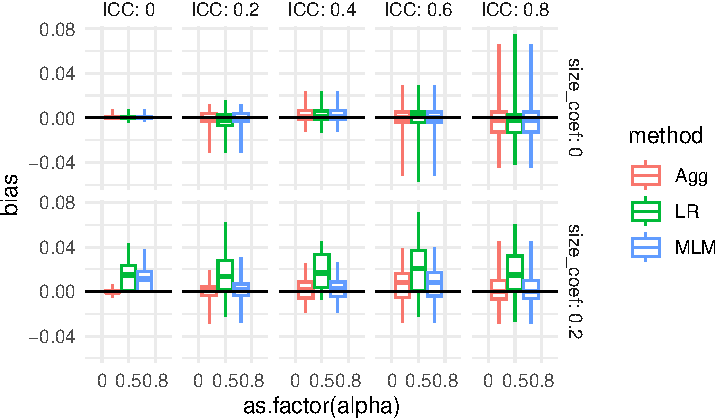
\includegraphics[width=0.75\linewidth]{Designing-Simulations-in-R_files/figure-latex/clusterRCT_plot_bias_v1-1} \end{center}

Each box is a collection of simulation trials. E.g., for \texttt{ICC\ =\ 0.6}, \texttt{size\_coef\ =\ 0.2}, and \texttt{alpha\ =\ 0.8} we have 9 scenarios representing the varying level 1 and level 2 sample sizes:

\begin{Shaded}
\begin{Highlighting}[]
\FunctionTok{filter}\NormalTok{( sres, ICC }\SpecialCharTok{==} \FloatTok{0.6}\NormalTok{, size\_coef }\SpecialCharTok{==} \FloatTok{0.2}\NormalTok{,}
\NormalTok{        alpha }\SpecialCharTok{==} \FloatTok{0.8}\NormalTok{, method}\SpecialCharTok{==}\StringTok{"Agg"}\NormalTok{ ) }\SpecialCharTok{\%\textgreater{}\%}
\NormalTok{  dplyr}\SpecialCharTok{::}\FunctionTok{select}\NormalTok{( n\_bar}\SpecialCharTok{:}\NormalTok{alpha, bias )}
\end{Highlighting}
\end{Shaded}

\begin{verbatim}
## # A tibble: 9 x 7
##   n_bar     J   ATE size_coef   ICC alpha     bias
##   <dbl> <dbl> <dbl>     <dbl> <dbl> <dbl>    <dbl>
## 1    20     5   0.2       0.2   0.6   0.8  0.00799
## 2    20    20   0.2       0.2   0.6   0.8 -0.0445 
## 3    20    80   0.2       0.2   0.6   0.8  0.0206 
## 4    80     5   0.2       0.2   0.6   0.8  0.111  
## 5    80    20   0.2       0.2   0.6   0.8 -0.0144 
## 6    80    80   0.2       0.2   0.6   0.8  0.0132 
## 7   320     5   0.2       0.2   0.6   0.8  0.151  
## 8   320    20   0.2       0.2   0.6   0.8  0.0361 
## 9   320    80   0.2       0.2   0.6   0.8  0.0394
\end{verbatim}

We are seeing a few outliers for some of the boxplots, suggesting that there are other factors driving bias. We could try bundling along different aspects to see:

\begin{Shaded}
\begin{Highlighting}[]
\FunctionTok{ggplot}\NormalTok{( sres, }\FunctionTok{aes}\NormalTok{( }\FunctionTok{as.factor}\NormalTok{(n\_bar), bias, }\AttributeTok{col=}\NormalTok{method, }\AttributeTok{group=}\FunctionTok{paste0}\NormalTok{(n\_bar,method) ) ) }\SpecialCharTok{+}
  \FunctionTok{facet\_grid}\NormalTok{( alpha }\SpecialCharTok{\textasciitilde{}}\NormalTok{  size\_coef, }\AttributeTok{labeller =}\NormalTok{ label\_both ) }\SpecialCharTok{+}
  \FunctionTok{geom\_boxplot}\NormalTok{(}\AttributeTok{coef =} \ConstantTok{Inf}\NormalTok{) }\SpecialCharTok{+}
  \FunctionTok{geom\_hline}\NormalTok{( }\AttributeTok{yintercept =} \DecValTok{0}\NormalTok{ ) }\SpecialCharTok{+}
  \FunctionTok{theme\_minimal}\NormalTok{()}
\end{Highlighting}
\end{Shaded}

\begin{center}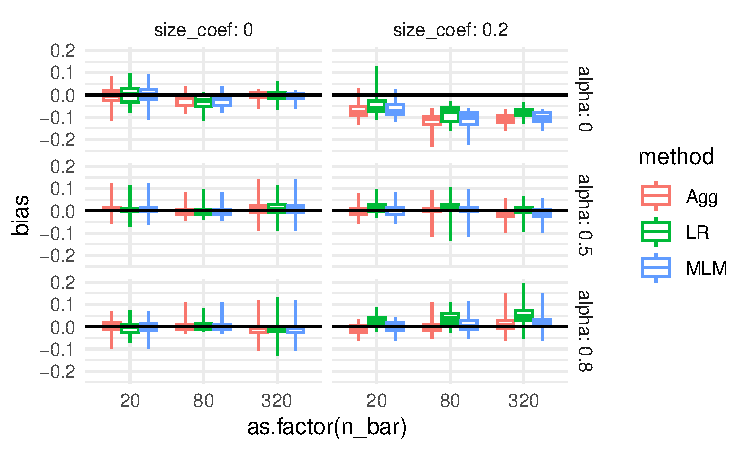
\includegraphics[width=0.75\linewidth]{Designing-Simulations-in-R_files/figure-latex/clusterRCT_plot_bias_v2-1} \end{center}

No progress there. Perhaps it is instability or MCSE.
We make a note to investigate further, later on.

\section{Aggregation}\label{aggregation}

The boxplots are hard for seeing trends.
Instead of bundling, we can therefore aggregate, to look at overall trends rather than individual simulation variation.
This is especially important if the number of replicates within each scenario is small, because then each scenario's performance is measured with a lot of error.

With aggregation, we average over some of the factors, collapsing our simulation results down to fewer moving parts.
This is better than having not had those factors in the first place!
Averaging over a factor is a more general answer than having not varied the factor at all.

For example, if we average across ICC and site variation, and see how the methods change performance as a function of \(J\), we would know that this is a general trend across a range of scenarios defined by different ICC and site variation levels.
Our conclusions would then be more general than if we picked a single ICC and amount of site variation: in this latter case we would not know if we would see our trend more broadly.

Also, with aggregation, we can have a smaller number of replications per factor combination.
The averaging will, in effect, give a lot more reps per aggregated performance measure.

A caution with aggregation is that it can be deceitful if you have scaling issues or extreme outliers.
With bias, our scale is fairly well set, so we are good!
But if we were aggregating standard errors over sample size, then the larger standard errors of the smaller sample size simulations (and the greater variability in estimating those standard errors) would swamp the standard errors of the larger sample sizes.
Usually, with aggregation, we want to average over something we believe will not change massively over the marginalized-out factors.
Alternatively, we can average over a relative measure, which tend to be more invariant and comparable across scenarios.

For our cluster RCT, we might aggregate as follows:

\begin{Shaded}
\begin{Highlighting}[]
\NormalTok{ssres }\OtherTok{\textless{}{-}} 
\NormalTok{  sres }\SpecialCharTok{\%\textgreater{}\%} 
  \FunctionTok{group\_by}\NormalTok{( ICC, method, alpha, size\_coef ) }\SpecialCharTok{\%\textgreater{}\%}
  \FunctionTok{summarise}\NormalTok{( }\AttributeTok{bias =} \FunctionTok{mean}\NormalTok{( bias ) )}

\FunctionTok{ggplot}\NormalTok{( ssres, }\FunctionTok{aes}\NormalTok{( ICC, bias, }\AttributeTok{col=}\NormalTok{method ) ) }\SpecialCharTok{+}
  \FunctionTok{facet\_grid}\NormalTok{( alpha }\SpecialCharTok{\textasciitilde{}}\NormalTok{  size\_coef, }\AttributeTok{labeller =}\NormalTok{ label\_both ) }\SpecialCharTok{+}
  \FunctionTok{geom\_point}\NormalTok{( }\AttributeTok{alpha=}\FloatTok{0.75}\NormalTok{ ) }\SpecialCharTok{+} 
  \FunctionTok{geom\_line}\NormalTok{( }\AttributeTok{alpha=}\FloatTok{0.75}\NormalTok{ ) }\SpecialCharTok{+}
  \FunctionTok{geom\_hline}\NormalTok{( }\AttributeTok{yintercept =} \DecValTok{0}\NormalTok{ ) }\SpecialCharTok{+}
  \FunctionTok{theme\_minimal}\NormalTok{()}
\end{Highlighting}
\end{Shaded}

\begin{center}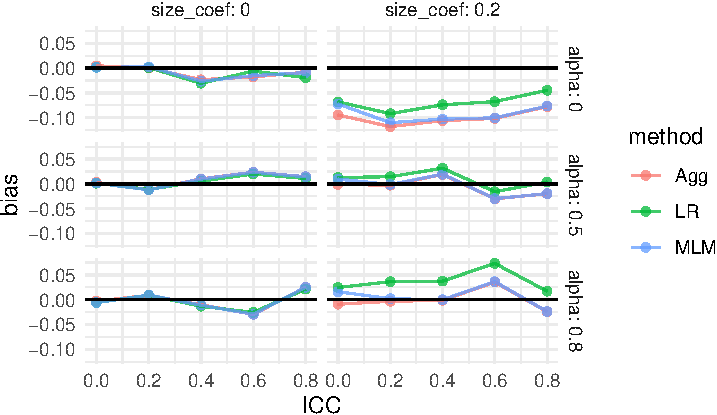
\includegraphics[width=0.75\linewidth]{Designing-Simulations-in-R_files/figure-latex/unnamed-chunk-151-1} \end{center}

This shows that site variation leads to greater bias, but only if the coefficient for size is nonzero.
We also see that all the estimators must be the same if site variation is 0, with the overplotted lines on the top row of the figure.

\section{Regression Summarization}\label{regression-summarization}

One can treat the simulation results as a dataset in its own right.
In this case we can regress a performance measure against the methods and various factor levels to get ``main effects'' of how the different levels impact performance holding the other levels constant.
The main effect of the method will tell us if a method is, on average, higher or lower than the baseline method.
The main effect of the factors will tell us if that factor impacts the performance measure.

These regressions can also include interactions between method and factor, to see if some factors impact different methods differently.
They can also include interactions between factors, which allows us to explore how the impact of a factor can matter more or less, depending on other aspects of the context.

For our cluster RCT, we might have, for example:

\begin{Shaded}
\begin{Highlighting}[]
\NormalTok{sres\_f }\OtherTok{=}\NormalTok{ sres }\SpecialCharTok{\%\textgreater{}\%}
  \FunctionTok{mutate}\NormalTok{( }\FunctionTok{across}\NormalTok{( }\FunctionTok{c}\NormalTok{( n\_bar, J, size\_coef, ICC, alpha ), factor ) )}

\NormalTok{M }\OtherTok{\textless{}{-}} \FunctionTok{lm}\NormalTok{( bias }\SpecialCharTok{\textasciitilde{}}\NormalTok{ (n\_bar }\SpecialCharTok{+}\NormalTok{ J }\SpecialCharTok{+}\NormalTok{ size\_coef }\SpecialCharTok{+}\NormalTok{ ICC }\SpecialCharTok{+}\NormalTok{ alpha) }\SpecialCharTok{*}\NormalTok{ method, }
         \AttributeTok{data =}\NormalTok{ sres\_f )}
\NormalTok{stargazer}\SpecialCharTok{::}\FunctionTok{stargazer}\NormalTok{(M, }\AttributeTok{type =} \StringTok{"text"}\NormalTok{,}
                     \AttributeTok{single.row =} \ConstantTok{TRUE}\NormalTok{ )}
\end{Highlighting}
\end{Shaded}

\begin{verbatim}
## 
## ==================================================
##                            Dependent variable:    
##                        ---------------------------
##                                   bias            
## --------------------------------------------------
## n_bar80                      -0.009 (0.007)       
## n_bar320                     -0.006 (0.007)       
## J20                           0.004 (0.007)       
## J80                           0.006 (0.007)       
## size_coef0.2                -0.035*** (0.006)     
## ICC0.2                       -0.004 (0.009)       
## ICC0.4                       -0.002 (0.009)       
## ICC0.6                       -0.003 (0.009)       
## ICC0.8                        0.001 (0.009)       
## alpha0.5                    0.055*** (0.007)      
## alpha0.8                    0.053*** (0.007)      
## methodLR                     -0.007 (0.014)       
## methodMLM                     0.006 (0.014)       
## n_bar80:methodLR             -0.001 (0.010)       
## n_bar320:methodLR             0.001 (0.010)       
## n_bar80:methodMLM            -0.001 (0.010)       
## n_bar320:methodMLM           -0.002 (0.010)       
## J20:methodLR                  0.006 (0.010)       
## J80:methodLR                  0.005 (0.010)       
## J20:methodMLM                 0.002 (0.010)       
## J80:methodMLM                 0.002 (0.010)       
## size_coef0.2:methodLR       0.030*** (0.008)      
## size_coef0.2:methodMLM        0.006 (0.008)       
## ICC0.2:methodLR               0.003 (0.013)       
## ICC0.4:methodLR              0.0004 (0.013)       
## ICC0.6:methodLR               0.005 (0.013)       
## ICC0.8:methodLR               0.002 (0.013)       
## ICC0.2:methodMLM             -0.006 (0.013)       
## ICC0.4:methodMLM             -0.008 (0.013)       
## ICC0.6:methodMLM             -0.008 (0.013)       
## ICC0.8:methodMLM             -0.008 (0.013)       
## alpha0.5:methodLR            -0.007 (0.010)       
## alpha0.8:methodLR             0.004 (0.010)       
## alpha0.5:methodMLM           -0.002 (0.010)       
## alpha0.8:methodMLM           -0.0003 (0.010)      
## Constant                    -0.034*** (0.010)     
## --------------------------------------------------
## Observations                       810            
## R2                                0.302           
## Adjusted R2                       0.270           
## Residual Std. Error         0.046 (df = 774)      
## F Statistic              9.547*** (df = 35; 774)  
## ==================================================
## Note:                  *p<0.1; **p<0.05; ***p<0.01
\end{verbatim}

We can quickly get a lot of features, and this approach can be hard to interpret. But picking out the significant coefficents does provide a lot of clues, rather rapidly.
E.g., many features interact with the LR method for bias. The other methods seem less impacted.

\section{Focus on subset, kick rest to supplement}\label{focus-on-subset-kick-rest-to-supplement}

Frequently researchers might simply filter the simulation results to a single factor level for some nuisance parameter.
For example, we might examine ICC of 0.20 only, as this is a ``reasonable'' value given substance matter knowledge.
We would then consider the other levels as a ``sensitivity'' analysis vaguely alluded to in our main report and placed elsewhere, such as an online supplemental appendix.

It would be our job, in this case, to verify that our reported findings on the main results indeed were echoed in our other, set-aside, simulation runs.

\section{Analyzing results when some trials have failed}\label{analyzing-results-when-some-trials-have-failed}

If methods fail, then this is something to investigate in its own right.
Ideally, failure is not too common, so we can drop those trials, or keep them, without really impacting our overall results.
But one should at least know what one is ignoring.

For example, in our cluster RCT, we know we have, at least sometimes, convergence issues.
We know that ICC is an important feature, so we can explore how often we get a convergence message by ICC level:

\begin{Shaded}
\begin{Highlighting}[]
\NormalTok{res }\SpecialCharTok{\%\textgreater{}\%} 
  \FunctionTok{group\_by}\NormalTok{( method, ICC ) }\SpecialCharTok{\%\textgreater{}\%}
  \FunctionTok{summarise}\NormalTok{( }\AttributeTok{message =} \FunctionTok{mean}\NormalTok{( message ) ) }\SpecialCharTok{\%\textgreater{}\%}
  \FunctionTok{pivot\_wider}\NormalTok{( }\AttributeTok{names\_from =} \StringTok{"method"}\NormalTok{, }\AttributeTok{values\_from=}\StringTok{"message"}\NormalTok{ )}
\end{Highlighting}
\end{Shaded}

\begin{verbatim}
## Warning: There were 15 warnings in `summarise()`.
## The first warning was:
## i In argument: `message = mean(message)`.
## i In group 1: `method = "Agg"` and `ICC = 0`.
## Caused by warning in `mean.default()`:
## ! argument is not numeric or logical: returning NA
## i Run `dplyr::last_dplyr_warnings()` to see the
##   14 remaining warnings.
\end{verbatim}

\begin{verbatim}
## # A tibble: 5 x 4
##     ICC   Agg    LR   MLM
##   <dbl> <dbl> <dbl> <dbl>
## 1   0      NA    NA    NA
## 2   0.2    NA    NA    NA
## 3   0.4    NA    NA    NA
## 4   0.6    NA    NA    NA
## 5   0.8    NA    NA    NA
\end{verbatim}

We see that when the ICC is 0 we get a lot of convergence issues, but as soon as we pull away from 0 it drops off considerably.
At this point we might decide to drop those runs with a message or keep them.
In this case, we decide to keep.
It shouldn't matter much in any case except the ICC = 0 case, and we know the convergence is due to trying to estimate a 0 variance, and thus is in some sense expected.
Furthermore, we know people using these methods would likely ignore these messages, and thus we are faithfully capturing how these methods would be used in practice.
We might eventually, however, want to do a separate analysis of the ICC = 0 context to see if the MLM approach actually falls apart, or if it is just throwing error messages.

\section{A demonstration of visualization}\label{a-demonstration-of-visualization}

We next explore a case study comparing different visualizations of the same performance metric (in this case, power).
The goal is to see how to examine a metric from several perspectives, and to see how to explore simulation results across scenarios.

For this example, we are going to look at a randomized experiment.
We will generate control potential outcomes, and then add a treatment effect to the treated units.
We assume the control group is normally distributed.
We will generate a random data set, estimate the
treatment effect by taking the difference in means and calculating the
associated standard error, and generating a \(p\)-value using the normal
approximation. (As we will see, this is not a good idea for small sample
size since we should be using a \(t\)-test style approach.)

Violating our usual modular approach, we ae going to have a single function that does an entire step: it generates two groups of the given sizes, one treatment and
one control, and then calculates the difference in means. It will then test
this difference using the normal approximation.

The function also calculates and returns the true effect size of the DGP as the true treatment
effect divided by the control standard deviation (useful for understanding
power, shown later on).

\begin{Shaded}
\begin{Highlighting}[]
\NormalTok{run.one }\OtherTok{=} \ControlFlowTok{function}\NormalTok{( nC, nT, sdC, tau, }\AttributeTok{mu =} \DecValTok{5}\NormalTok{, }\AttributeTok{sdTau =} \DecValTok{0}\NormalTok{ ) \{}
\NormalTok{  Y0 }\OtherTok{=}\NormalTok{ mu }\SpecialCharTok{+} \FunctionTok{rnorm}\NormalTok{( nC, }\AttributeTok{sd=}\NormalTok{sdC )}
\NormalTok{  Y1 }\OtherTok{=}\NormalTok{ mu }\SpecialCharTok{+} \FunctionTok{rnorm}\NormalTok{( nT, }\AttributeTok{sd=}\NormalTok{sdC ) }\SpecialCharTok{+}\NormalTok{ tau }\SpecialCharTok{+} \FunctionTok{rnorm}\NormalTok{( nT, }\AttributeTok{sd=}\NormalTok{sdTau )}

\NormalTok{  tau.hat }\OtherTok{=} \FunctionTok{mean}\NormalTok{( Y1 ) }\SpecialCharTok{{-}} \FunctionTok{mean}\NormalTok{( Y0 )}
\NormalTok{  SE.hat }\OtherTok{=} \FunctionTok{sqrt}\NormalTok{( }\FunctionTok{var}\NormalTok{( Y0 ) }\SpecialCharTok{/}\NormalTok{ ( nC ) }\SpecialCharTok{+} \FunctionTok{var}\NormalTok{( Y1 ) }\SpecialCharTok{/}\NormalTok{ ( nT ) )}

\NormalTok{  z }\OtherTok{=}\NormalTok{ tau.hat }\SpecialCharTok{/}\NormalTok{ SE.hat}
\NormalTok{  pv }\OtherTok{=} \DecValTok{2} \SpecialCharTok{*}\NormalTok{ (}\DecValTok{1} \SpecialCharTok{{-}} \FunctionTok{pnorm}\NormalTok{( }\FunctionTok{abs}\NormalTok{( z ) ))}

  \FunctionTok{data.frame}\NormalTok{( }\AttributeTok{tau.hat =}\NormalTok{ tau.hat, }\AttributeTok{SE.hat =}\NormalTok{ SE.hat, }\AttributeTok{z=}\NormalTok{z, }\AttributeTok{p.value=}\NormalTok{pv )}
\NormalTok{\}}
\end{Highlighting}
\end{Shaded}

Our function generates a data set, analyzes it, and give us back a variety
of results as a one-row dataframe, as per usual:

\begin{Shaded}
\begin{Highlighting}[]
\FunctionTok{run.one}\NormalTok{( }\AttributeTok{nT=}\DecValTok{5}\NormalTok{, }\AttributeTok{nC=}\DecValTok{10}\NormalTok{, }\AttributeTok{sdC=}\DecValTok{1}\NormalTok{, }\AttributeTok{tau=}\FloatTok{0.5}\NormalTok{ )}
\end{Highlighting}
\end{Shaded}

\begin{verbatim}
##     tau.hat    SE.hat          z   p.value
## 1 -0.246767 0.6607213 -0.3734812 0.7087903
\end{verbatim}

In this case, our results are a mix of the parameters and estimated quantities.

We then write a function that runs our single trial multiple times and
summarizes the results:

\begin{Shaded}
\begin{Highlighting}[]
\NormalTok{run.experiment }\OtherTok{=} \ControlFlowTok{function}\NormalTok{( nC, nT, sdC, tau, }\AttributeTok{mu =} \DecValTok{5}\NormalTok{, }\AttributeTok{sdTau =} \DecValTok{0}\NormalTok{, }\AttributeTok{R =} \DecValTok{500}\NormalTok{ ) \{}

\NormalTok{  eres }\OtherTok{=} \FunctionTok{replicate}\NormalTok{( R, }\FunctionTok{run.one}\NormalTok{( nC, nT, sdC, tau, }\AttributeTok{sdTau=}\NormalTok{sdTau, }\AttributeTok{mu=}\NormalTok{mu ), }
                    \AttributeTok{simplify=}\ConstantTok{FALSE}\NormalTok{ )}
\NormalTok{  eres }\OtherTok{=} \FunctionTok{bind\_rows}\NormalTok{( eres )}
\NormalTok{  eres }\SpecialCharTok{\%\textgreater{}\%} \FunctionTok{summarise}\NormalTok{( }\AttributeTok{E.tau.hat =} \FunctionTok{mean}\NormalTok{( tau.hat ),}
                      \AttributeTok{E.SE.hat =} \FunctionTok{mean}\NormalTok{( SE.hat ),}
                      \AttributeTok{power =} \FunctionTok{mean}\NormalTok{( p.value }\SpecialCharTok{\textless{}=} \FloatTok{0.05}\NormalTok{ ) ) }\SpecialCharTok{\%\textgreater{}\%}
    \FunctionTok{mutate}\NormalTok{( }\AttributeTok{nC=}\NormalTok{nC, }\AttributeTok{nT=}\NormalTok{nT, }\AttributeTok{sdC=}\NormalTok{sdC, }\AttributeTok{tau=}\NormalTok{tau, }\AttributeTok{mu=}\NormalTok{mu, }\AttributeTok{sdTau=}\NormalTok{sdTau, }\AttributeTok{R=}\NormalTok{R )}
\NormalTok{\}}
\end{Highlighting}
\end{Shaded}

For performance, we have the average average treatment effect estimate \texttt{E.tau.hat},
the average Standard Error estimate \texttt{E.SE.hat},
and the power \texttt{power} (defined as the percent of time we reject at
alpha=0.05, i.e., the percent of times our \(p\)-value was less than our 0.05
threshold):

Our function also adds in the details of the simulation (the parameters we passed
to the \texttt{run.one()} call). This is an easy way to keep track of things.

We test our function to see what we get:

\begin{Shaded}
\begin{Highlighting}[]
\FunctionTok{run.experiment}\NormalTok{( }\DecValTok{10}\NormalTok{, }\DecValTok{3}\NormalTok{, }\DecValTok{1}\NormalTok{, }\FloatTok{0.5}\NormalTok{, }\DecValTok{5}\NormalTok{, }\FloatTok{0.2}\NormalTok{ )}
\end{Highlighting}
\end{Shaded}

\begin{verbatim}
##   E.tau.hat  E.SE.hat power nC nT sdC tau mu
## 1  0.497077 0.6284977 0.218 10  3   1 0.5  5
##   sdTau   R
## 1   0.2 500
\end{verbatim}

We next use the above to run a \emph{multi-factor simulation experiment}. We are
going to vary four factors: control group size, treatment group size,
standard deviation of the units, and the treatment effect.

\begin{Shaded}
\begin{Highlighting}[]
\NormalTok{nC }\OtherTok{=} \FunctionTok{c}\NormalTok{( }\DecValTok{2}\NormalTok{, }\DecValTok{4}\NormalTok{, }\DecValTok{7}\NormalTok{, }\DecValTok{10}\NormalTok{, }\DecValTok{50}\NormalTok{, }\DecValTok{500}\NormalTok{ )}
\NormalTok{nT }\OtherTok{=} \FunctionTok{c}\NormalTok{( }\DecValTok{2}\NormalTok{, }\DecValTok{4}\NormalTok{, }\DecValTok{7}\NormalTok{, }\DecValTok{10}\NormalTok{, }\DecValTok{50}\NormalTok{, }\DecValTok{500}\NormalTok{ )}
\NormalTok{sdC }\OtherTok{=} \FunctionTok{c}\NormalTok{( }\DecValTok{1}\NormalTok{ )}
\NormalTok{tau }\OtherTok{=} \FunctionTok{c}\NormalTok{( }\DecValTok{0}\NormalTok{, }\FloatTok{0.5}\NormalTok{, }\DecValTok{1}\NormalTok{ )}
\NormalTok{sdTau }\OtherTok{=} \FunctionTok{c}\NormalTok{( }\DecValTok{0}\NormalTok{, }\FloatTok{0.5}\NormalTok{ )}

\NormalTok{experiments }\OtherTok{=} \FunctionTok{expand\_grid}\NormalTok{( }\AttributeTok{nC=}\NormalTok{nC, }\AttributeTok{nT=}\NormalTok{nT, }\AttributeTok{sdC=}\NormalTok{sdC, }\AttributeTok{tau=}\NormalTok{tau, }\AttributeTok{sdTau =}\NormalTok{ sdTau )}
\NormalTok{experiments}
\end{Highlighting}
\end{Shaded}

\begin{verbatim}
## # A tibble: 216 x 5
##       nC    nT   sdC   tau sdTau
##    <dbl> <dbl> <dbl> <dbl> <dbl>
##  1     2     2     1   0     0  
##  2     2     2     1   0     0.5
##  3     2     2     1   0.5   0  
##  4     2     2     1   0.5   0.5
##  5     2     2     1   1     0  
##  6     2     2     1   1     0.5
##  7     2     4     1   0     0  
##  8     2     4     1   0     0.5
##  9     2     4     1   0.5   0  
## 10     2     4     1   0.5   0.5
## # i 206 more rows
\end{verbatim}

We next run an experiment for each row of our dataframe of experiment factor
combinations, and save the results.
Note our method of adding the design parametes into our results makes this step arguably moe clean than some of the other templates we have seen.

\begin{Shaded}
\begin{Highlighting}[]
\NormalTok{exp.res }\OtherTok{\textless{}{-}}\NormalTok{ experiments }\SpecialCharTok{\%\textgreater{}\%} \FunctionTok{pmap\_df}\NormalTok{( run.experiment, }\AttributeTok{R=}\DecValTok{2000}\NormalTok{ )}
\FunctionTok{dir.create}\NormalTok{(}\StringTok{"results"}\NormalTok{, }\AttributeTok{showWarnings =} \ConstantTok{FALSE}\NormalTok{ )}
\FunctionTok{saveRDS}\NormalTok{( exp.res, }\AttributeTok{file=}\StringTok{"results/Neyman\_RCT\_results.rds"}\NormalTok{ )}
\end{Highlighting}
\end{Shaded}

The \texttt{R=500} after \texttt{run.experiment} passes the \emph{same} parameter of \(R=500\) to each
run (we run the same number of trials for each experiment).
We can put it there rather than have it be a column in our list of factors to run.

Here is a peek at our results:

\begin{Shaded}
\begin{Highlighting}[]
\FunctionTok{head}\NormalTok{( exp.res )}
\end{Highlighting}
\end{Shaded}

\begin{verbatim}
##      E.tau.hat  E.SE.hat  power nC nT sdC tau mu
## 1 -0.001525155 0.8818917 0.1975  2  2   1 0.0  5
## 2 -0.026286662 0.9307269 0.1915  2  2   1 0.0  5
## 3  0.485430674 0.8861287 0.2185  2  2   1 0.5  5
## 4  0.452375661 0.9363909 0.2095  2  2   1 0.5  5
## 5  1.029038283 0.8915091 0.3120  2  2   1 1.0  5
## 6  0.957434064 0.9347139 0.3025  2  2   1 1.0  5
##   sdTau    R
## 1   0.0 2000
## 2   0.5 2000
## 3   0.0 2000
## 4   0.5 2000
## 5   0.0 2000
## 6   0.5 2000
\end{verbatim}

\subsection{The initial analysis}\label{the-initial-analysis}

We are ready to analyze.

We start with plotting.
Plotting is always a good way to vizualize simulation results.
We first make
our tau into a factor, so \texttt{ggplot} behaves, and then plot all our
experiments as two rows based on one factor (\texttt{sdTau}) with the columns being
another (\texttt{nT}). (This style of plotting a bunch of small plots is called
``many multiples'' and is beloved by Tufte.) Within each plot we have the
x-axis for one factor (\texttt{nC}) and multiple lines for the final factor (\texttt{tau}).
The \(y\)-axis is our outcome of interest, power. We add a 0.05 line to show
when we are rejecting at rates above our nominal \(\alpha\). This plot shows
the relationship of 5 variables.

\begin{Shaded}
\begin{Highlighting}[]
\NormalTok{exp.res }\OtherTok{=}\NormalTok{ exp.res }\SpecialCharTok{\%\textgreater{}\%} \FunctionTok{mutate}\NormalTok{( }\AttributeTok{tau =} \FunctionTok{as.factor}\NormalTok{( tau ) )}
\FunctionTok{ggplot}\NormalTok{( exp.res, }\FunctionTok{aes}\NormalTok{( }\AttributeTok{x=}\NormalTok{nC, }\AttributeTok{y=}\NormalTok{power, }\AttributeTok{group=}\NormalTok{tau, }\AttributeTok{col=}\NormalTok{tau ) ) }\SpecialCharTok{+}
  \FunctionTok{facet\_grid}\NormalTok{( sdTau }\SpecialCharTok{\textasciitilde{}}\NormalTok{ nT, }\AttributeTok{labeller=}\NormalTok{label\_both ) }\SpecialCharTok{+}
  \FunctionTok{geom\_point}\NormalTok{() }\SpecialCharTok{+} \FunctionTok{geom\_line}\NormalTok{() }\SpecialCharTok{+}
  \FunctionTok{scale\_x\_log10}\NormalTok{() }\SpecialCharTok{+}
  \FunctionTok{geom\_hline}\NormalTok{( }\AttributeTok{yintercept=}\FloatTok{0.05}\NormalTok{, }\AttributeTok{col=}\StringTok{"black"}\NormalTok{, }\AttributeTok{lty=}\DecValTok{2}\NormalTok{)}
\end{Highlighting}
\end{Shaded}

\begin{center}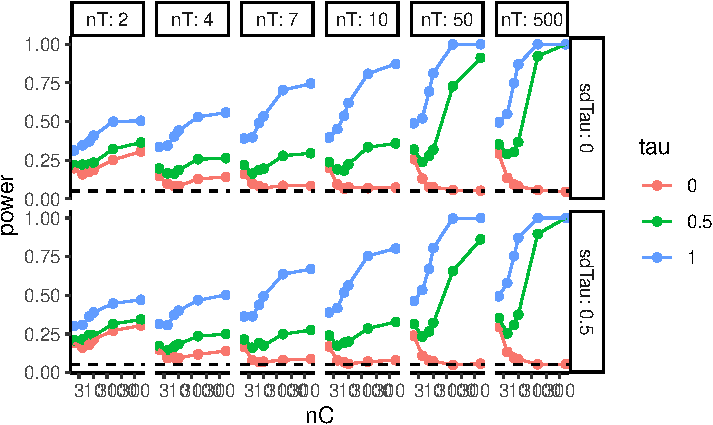
\includegraphics[width=0.75\linewidth]{Designing-Simulations-in-R_files/figure-latex/unnamed-chunk-159-1} \end{center}

We ae looking at power for different control and treatment group sizes. The tau is our treatment effect, and so for \(\tau = 0\) we are looking at validity (false rejection of the null) and for the other \(\tau\) power (noticing an effect when it is there).
Notice that we are seeing elevated rejection rates under the null for small and even moderate sample sizes!

\subsection{Focusing on validity}\label{focusing-on-validity}

We can zoom in on specific simulations run, to get some more detail
such as estimated power under the null for larger groups. Here we check
and we are seeing rejection rates (\texttt{power}) of around 0.05, which is what we want.

\begin{Shaded}
\begin{Highlighting}[]
\FunctionTok{filter}\NormalTok{( exp.res, tau}\SpecialCharTok{==}\DecValTok{0}\NormalTok{, nT }\SpecialCharTok{\textgreater{}=} \DecValTok{50}\NormalTok{, nC }\SpecialCharTok{\textgreater{}=} \DecValTok{50}\NormalTok{ ) }\SpecialCharTok{\%\textgreater{}\%}
\NormalTok{  knitr}\SpecialCharTok{::}\FunctionTok{kable}\NormalTok{(}\AttributeTok{digits=}\DecValTok{2}\NormalTok{)}
\end{Highlighting}
\end{Shaded}

\begin{tabular}{r|r|r|r|r|r|l|r|r|r}
\hline
E.tau.hat & E.SE.hat & power & nC & nT & sdC & tau & mu & sdTau & R\\
\hline
0 & 0.20 & 0.06 & 50 & 50 & 1 & 0 & 5 & 0.0 & 2000\\
\hline
0 & 0.21 & 0.05 & 50 & 50 & 1 & 0 & 5 & 0.5 & 2000\\
\hline
0 & 0.15 & 0.06 & 50 & 500 & 1 & 0 & 5 & 0.0 & 2000\\
\hline
0 & 0.15 & 0.05 & 50 & 500 & 1 & 0 & 5 & 0.5 & 2000\\
\hline
0 & 0.15 & 0.05 & 500 & 50 & 1 & 0 & 5 & 0.0 & 2000\\
\hline
0 & 0.16 & 0.06 & 500 & 50 & 1 & 0 & 5 & 0.5 & 2000\\
\hline
0 & 0.06 & 0.04 & 500 & 500 & 1 & 0 & 5 & 0.0 & 2000\\
\hline
0 & 0.07 & 0.06 & 500 & 500 & 1 & 0 & 5 & 0.5 & 2000\\
\hline
\end{tabular}

We can get fancy and look at rejection rate (power under \texttt{tau\ =\ 0}) as a
function of both nC and nT using an interaction-style plot where we average over the other variables:

\begin{Shaded}
\begin{Highlighting}[]
\NormalTok{exp.res.rej }\OtherTok{\textless{}{-}}\NormalTok{ exp.res }\SpecialCharTok{\%\textgreater{}\%} \FunctionTok{filter}\NormalTok{( tau }\SpecialCharTok{==} \DecValTok{0}\NormalTok{ ) }\SpecialCharTok{\%\textgreater{}\%}
  \FunctionTok{group\_by}\NormalTok{( nC, nT ) }\SpecialCharTok{\%\textgreater{}\%}
  \FunctionTok{summarize}\NormalTok{( }\AttributeTok{power =} \FunctionTok{mean}\NormalTok{( power ) )}

\NormalTok{exp.res.rej }\OtherTok{=} \FunctionTok{mutate}\NormalTok{( exp.res.rej, }\AttributeTok{power =} \FunctionTok{round}\NormalTok{( power }\SpecialCharTok{*} \DecValTok{100}\NormalTok{ ) )}

\FunctionTok{ggplot}\NormalTok{( exp.res.rej, }\FunctionTok{aes}\NormalTok{( }\AttributeTok{x=}\NormalTok{nC, }\AttributeTok{y=}\NormalTok{power, }\AttributeTok{group=}\NormalTok{nT, }\AttributeTok{col=}\FunctionTok{as.factor}\NormalTok{(nT) ) ) }\SpecialCharTok{+}
  \FunctionTok{geom\_point}\NormalTok{() }\SpecialCharTok{+} \FunctionTok{geom\_line}\NormalTok{() }\SpecialCharTok{+}
  \FunctionTok{geom\_hline}\NormalTok{( }\AttributeTok{yintercept =} \DecValTok{5}\NormalTok{ ) }\SpecialCharTok{+}
  \FunctionTok{scale\_y\_continuous}\NormalTok{( }\AttributeTok{limits =} \FunctionTok{c}\NormalTok{( }\DecValTok{0}\NormalTok{, }\DecValTok{40}\NormalTok{ ) ) }\SpecialCharTok{+}
  \FunctionTok{scale\_x\_log10}\NormalTok{( }\AttributeTok{breaks =} \FunctionTok{unique}\NormalTok{( exp.res.rej}\SpecialCharTok{$}\NormalTok{nC ) ) }\SpecialCharTok{+}
  \FunctionTok{labs}\NormalTok{( }\AttributeTok{x =} \StringTok{"\# C"}\NormalTok{, }\AttributeTok{y =} \StringTok{"Power"}\NormalTok{, }\AttributeTok{colour =} \StringTok{"\# T"}\NormalTok{ )}
\end{Highlighting}
\end{Shaded}

\begin{center}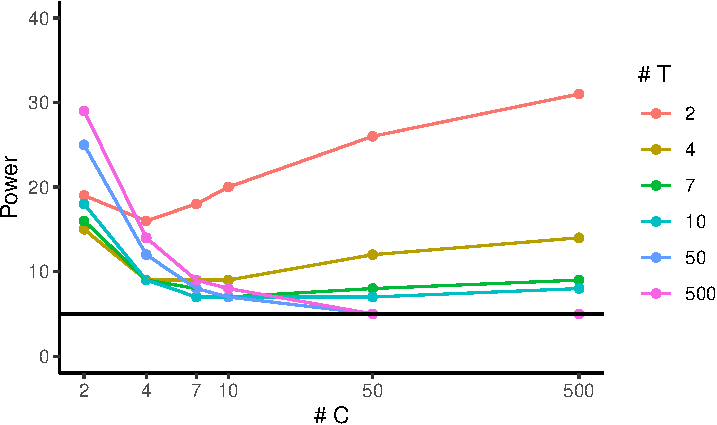
\includegraphics[width=0.75\linewidth]{Designing-Simulations-in-R_files/figure-latex/plot_interaction_Results-1} \end{center}

This plot focuses on the validity of our test.
It shows that we have massively elevated rates when either the number of treated or control units is small (10 or below).
It also shows that as the size of one group increases, if the other is small our rejection rates climb! Note how for 4 control units, the \(n_T = 500\) line is above the others (except for the \(n_T = 2\) line).

\subsection{Looking at main effects}\label{looking-at-main-effects}

We can ignore all the other factors while we look at one specific factor of interest.
This is looking at the \textbf{main effect} or \textbf{marginal effect} of the factor.

The easy way to do this is to let \texttt{ggplot} smooth our individual points on a
plot. Be sure to also plot the individual points to see variation, however.

\begin{Shaded}
\begin{Highlighting}[]
\FunctionTok{ggplot}\NormalTok{( exp.res, }\FunctionTok{aes}\NormalTok{( }\AttributeTok{x=}\NormalTok{nC, }\AttributeTok{y=}\NormalTok{power, }\AttributeTok{group=}\NormalTok{tau, }\AttributeTok{col=}\NormalTok{tau ) ) }\SpecialCharTok{+}
  \FunctionTok{geom\_jitter}\NormalTok{( }\AttributeTok{width=}\FloatTok{0.02}\NormalTok{, }\AttributeTok{height=}\DecValTok{0}\NormalTok{, }\AttributeTok{alpha=}\FloatTok{0.5}\NormalTok{ ) }\SpecialCharTok{+}
  \FunctionTok{geom\_smooth}\NormalTok{( }\AttributeTok{se =} \ConstantTok{FALSE}\NormalTok{ ) }\SpecialCharTok{+}
  \FunctionTok{scale\_x\_log10}\NormalTok{( }\AttributeTok{breaks=}\NormalTok{nC) }\SpecialCharTok{+}
  \FunctionTok{geom\_hline}\NormalTok{( }\AttributeTok{yintercept=}\FloatTok{0.05}\NormalTok{, }\AttributeTok{col=}\StringTok{"black"}\NormalTok{, }\AttributeTok{lty=}\DecValTok{2}\NormalTok{)}
\end{Highlighting}
\end{Shaded}

\begin{center}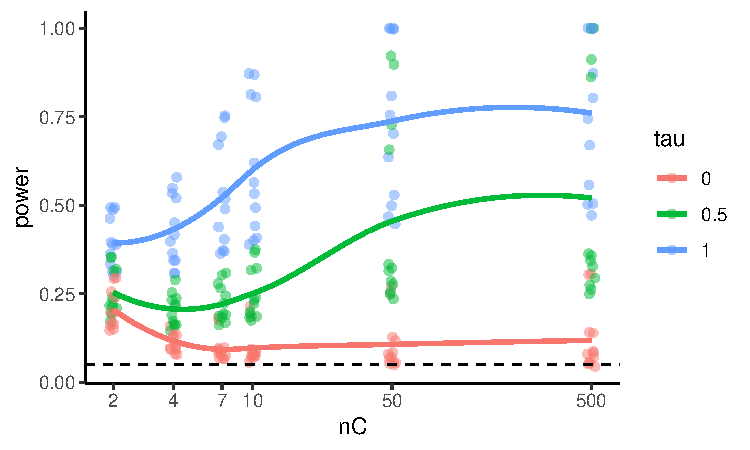
\includegraphics[width=0.75\linewidth]{Designing-Simulations-in-R_files/figure-latex/plotPool-1} \end{center}

Note how we see our individual runs that we marginalize over as the dots.

To look at our main effects we can also summarize our results, averaging our
experimental runs across other factor levels. For example, in the code below
we average over the different treatment group sizes and standard deviations,
and plot the marginalized results.

To marginalize, we group by the things we want to keep. \texttt{summarise()} then
averages over the things we want to get rid of.

\begin{Shaded}
\begin{Highlighting}[]
\NormalTok{exp.res.sum }\OtherTok{=}\NormalTok{ exp.res }\SpecialCharTok{\%\textgreater{}\%} \FunctionTok{group\_by}\NormalTok{( nC, tau ) }\SpecialCharTok{\%\textgreater{}\%}
  \FunctionTok{summarise}\NormalTok{( }\AttributeTok{power =} \FunctionTok{mean}\NormalTok{( power ) )}
\FunctionTok{head}\NormalTok{( exp.res.sum )}
\end{Highlighting}
\end{Shaded}

\begin{verbatim}
## # A tibble: 6 x 3
## # Groups:   nC [2]
##      nC tau   power
##   <dbl> <fct> <dbl>
## 1     2 0     0.205
## 2     2 0.5   0.254
## 3     2 1     0.395
## 4     4 0     0.114
## 5     4 0.5   0.204
## 6     4 1     0.427
\end{verbatim}

\begin{Shaded}
\begin{Highlighting}[]
\FunctionTok{ggplot}\NormalTok{( exp.res.sum, }\FunctionTok{aes}\NormalTok{( }\AttributeTok{x=}\NormalTok{nC, }\AttributeTok{y=}\NormalTok{power, }\AttributeTok{group=}\NormalTok{tau, }\AttributeTok{col=}\NormalTok{tau ) ) }\SpecialCharTok{+}
  \FunctionTok{geom\_line}\NormalTok{() }\SpecialCharTok{+} \FunctionTok{geom\_point}\NormalTok{() }\SpecialCharTok{+}
  \FunctionTok{scale\_x\_log10}\NormalTok{( }\AttributeTok{breaks=}\NormalTok{nC) }\SpecialCharTok{+}
  \FunctionTok{geom\_hline}\NormalTok{( }\AttributeTok{yintercept=}\FloatTok{0.05}\NormalTok{, }\AttributeTok{col=}\StringTok{"black"}\NormalTok{, }\AttributeTok{lty=}\DecValTok{2}\NormalTok{)}
\end{Highlighting}
\end{Shaded}

\begin{center}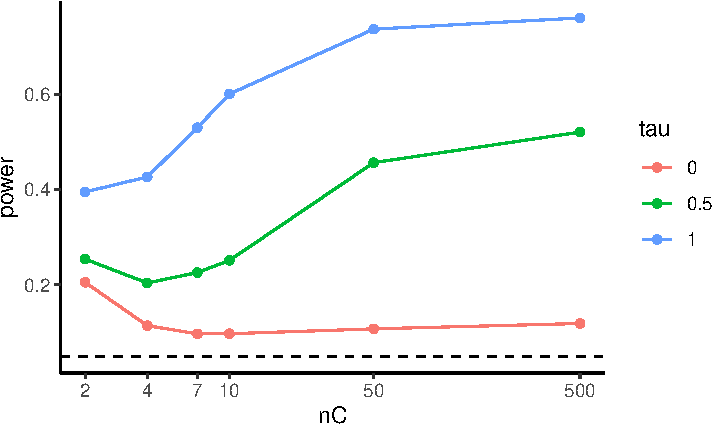
\includegraphics[width=0.75\linewidth]{Designing-Simulations-in-R_files/figure-latex/plotCollapse-1} \end{center}

We can try to get clever and look at other aspects of our experimental runs.
The above suggests that the smaller of the two groups is dictating things
going awry, in terms of elevated rejection rates under the null. We can also
look at things in terms of some other more easily interpretable parameter
(here we switch to effect size instead of raw treatment effect).

Given this, we might decide to look at total sample size or the smaller of
the two groups sample size and make plots that way (we are also subsetting to
just the \texttt{sd=1} cases as there is nothing really different about the two
options; we probably should average across but this could reduce clarity of
the presentation of results):

\begin{Shaded}
\begin{Highlighting}[]
\NormalTok{exp.res }\OtherTok{\textless{}{-}}\NormalTok{ exp.res }\SpecialCharTok{\%\textgreater{}\%} \FunctionTok{mutate}\NormalTok{( }\AttributeTok{n =}\NormalTok{ nC }\SpecialCharTok{+}\NormalTok{ nT,}
                               \AttributeTok{n.min =} \FunctionTok{pmin}\NormalTok{( nC, nT ) )}
\end{Highlighting}
\end{Shaded}

\begin{Shaded}
\begin{Highlighting}[]
\FunctionTok{ggplot}\NormalTok{( exp.res, }\FunctionTok{aes}\NormalTok{( }\AttributeTok{x=}\NormalTok{n, }\AttributeTok{y=}\NormalTok{power, }\AttributeTok{group=}\NormalTok{tau, }\AttributeTok{col=}\NormalTok{tau ) ) }\SpecialCharTok{+}
  \FunctionTok{geom\_jitter}\NormalTok{( }\AttributeTok{width=}\FloatTok{0.05}\NormalTok{, }\AttributeTok{height=}\DecValTok{0}\NormalTok{) }\SpecialCharTok{+}
  \FunctionTok{geom\_smooth}\NormalTok{( }\AttributeTok{se =} \ConstantTok{FALSE}\NormalTok{, }\AttributeTok{span =} \DecValTok{1}\NormalTok{) }\SpecialCharTok{+}
  \FunctionTok{scale\_x\_log10}\NormalTok{() }\SpecialCharTok{+}
  \FunctionTok{geom\_hline}\NormalTok{( }\AttributeTok{yintercept=}\FloatTok{0.05}\NormalTok{, }\AttributeTok{col=}\StringTok{"black"}\NormalTok{, }\AttributeTok{lty=}\DecValTok{2}\NormalTok{) }\SpecialCharTok{+}
  \FunctionTok{labs}\NormalTok{( }\AttributeTok{title =} \StringTok{"Total sample size"}\NormalTok{ )}
\end{Highlighting}
\end{Shaded}

\begin{center}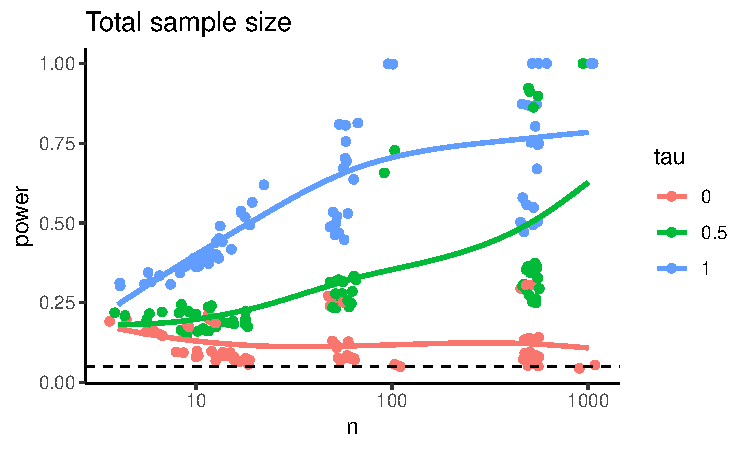
\includegraphics[width=0.75\linewidth]{Designing-Simulations-in-R_files/figure-latex/plotA-1} \end{center}

\begin{Shaded}
\begin{Highlighting}[]
\FunctionTok{ggplot}\NormalTok{( exp.res, }\FunctionTok{aes}\NormalTok{( }\AttributeTok{x=}\NormalTok{n.min, }\AttributeTok{y=}\NormalTok{power, }\AttributeTok{group=}\NormalTok{tau, }\AttributeTok{col=}\NormalTok{tau ) ) }\SpecialCharTok{+}
  \FunctionTok{geom\_jitter}\NormalTok{( }\AttributeTok{width=}\FloatTok{0.05}\NormalTok{, }\AttributeTok{height=}\DecValTok{0}\NormalTok{) }\SpecialCharTok{+}
  \FunctionTok{geom\_smooth}\NormalTok{( }\AttributeTok{se =} \ConstantTok{FALSE}\NormalTok{, }\AttributeTok{span =} \DecValTok{1}\NormalTok{) }\SpecialCharTok{+}
  \FunctionTok{scale\_x\_log10}\NormalTok{() }\SpecialCharTok{+}
  \FunctionTok{geom\_hline}\NormalTok{( }\AttributeTok{yintercept=}\FloatTok{0.05}\NormalTok{, }\AttributeTok{col=}\StringTok{"black"}\NormalTok{, }\AttributeTok{lty=}\DecValTok{2}\NormalTok{) }\SpecialCharTok{+}
  \FunctionTok{labs}\NormalTok{( }\AttributeTok{title =} \StringTok{"Minimum group size"}\NormalTok{ )}
\end{Highlighting}
\end{Shaded}

\begin{center}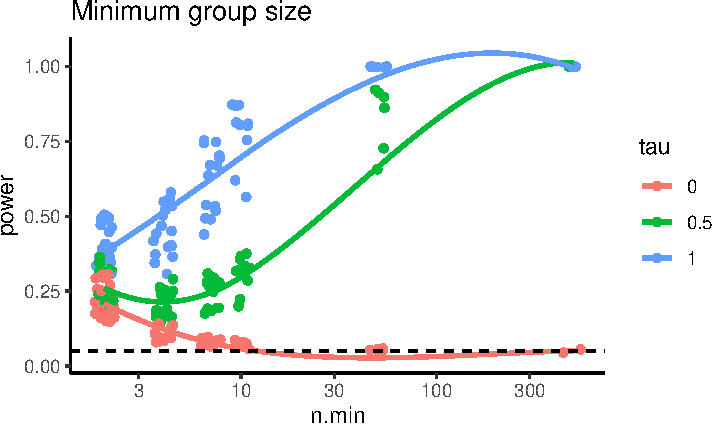
\includegraphics[width=0.75\linewidth]{Designing-Simulations-in-R_files/figure-latex/plotB-1} \end{center}

Note the few observations out in the high \texttt{n.min} region for the second
plot---this plot is a bit strange in that the different levels along the
x-axis are assymetric with respect to each other. It is not balanced.

\subsection{Recap}\label{recap}

Overall, this exploration demonstrates the process of looking at a single performance metric (power) and refining a series of plots to get a sense of what the simulation is taking us.
There are many different plots we might choose, and this depends on the messages we are trying to convey.

The key is to explore, and see what you can learn!

\section{Exercises}\label{exercises-6}

\begin{enumerate}
\def\labelenumi{\arabic{enumi})}
\tightlist
\item
  For our cluster RCT, use the simulation results to assess how much better (or worse) the different methods are to each other in terms of confidence interval coverage. What scenarios tend to result in the worst coverage?
\end{enumerate}

\chapter{Case study: Comparing different estimators}\label{case-study-comparing-different-estimators}

\emph{Features of this case study}
- Calculating performance metrics by estimator using tidyverse.
- Visualization of simulation results.
- Construction of the classic Bias + SE + RMSE performance plot.

In this case study we examine a simulation where we wish to compare different forms of
estimator for estimating the same thing. We still generate data, evaluate it,
and see how well our evaluation works. The difference is we now evaluate it
multiple ways, storing how the different ways work.

For our simple working example we are going to compare estimation of the
center of a symmetric distribution via mean, trimmed mean, and median (so the
mean and median are the same). These are the three estimation strategies
that we might be comparing in a paper (pretend we have ``invented'' the trimmed
mean and want to demonstrate its utility).

We are, as usual, going to break building this simulation evaluation down into lots of
functions to show the general framework. This framework can readily be
extended to more complicated simulation studies.
This case study illustrates how methodologists might compare different strategies for estimation, and is
closest to what we might see in the ``simulation'' section of a stats paper.

\section{The data generating process}\label{the-data-generating-process-1}

For our data-generation function we will use the scaled \(t\)-distribution so
the standard deviation will always be 1 but we will have different fatness of
tails (high chance of outliers):

\begin{Shaded}
\begin{Highlighting}[]
\NormalTok{gen.data }\OtherTok{=} \ControlFlowTok{function}\NormalTok{( n, df0 ) \{}
    \FunctionTok{rt}\NormalTok{( n, }\AttributeTok{df=}\NormalTok{df0 ) }\SpecialCharTok{/} \FunctionTok{sqrt}\NormalTok{( df0 }\SpecialCharTok{/}\NormalTok{ (df0}\DecValTok{{-}2}\NormalTok{) )}
\NormalTok{\}}
\end{Highlighting}
\end{Shaded}

The variance of a \(t\) is \(df/(df-2)\), so if we divide our observations by the
square root of this, we will standardize them so they have unit variance.
See, the standard deviation is 1 (up to random error, and as long as df0 \textgreater{}
2)!:

\begin{Shaded}
\begin{Highlighting}[]
\FunctionTok{sd}\NormalTok{( }\FunctionTok{gen.data}\NormalTok{( }\DecValTok{100000}\NormalTok{, }\AttributeTok{df0 =} \DecValTok{3}\NormalTok{ ) )}
\end{Highlighting}
\end{Shaded}

\begin{verbatim}
## [1] 1.01542
\end{verbatim}

(Normally our data generation code would be a bit more fancy.)

We next define the parameter we want (in our case this is the mean, is what
we are trying to estimate):

\begin{Shaded}
\begin{Highlighting}[]
\NormalTok{mu }\OtherTok{=} \DecValTok{0}
\end{Highlighting}
\end{Shaded}

\section{The data analysis methods}\label{the-data-analysis-methods}

We then write a function that takes data and uses all our different
estimators on it. We return a data frame of the three estimates, with each
row being one of our estimators. This is useful if our estimators return an
estimate and a standard error, for example.

\begin{Shaded}
\begin{Highlighting}[]
\NormalTok{analyze.data }\OtherTok{=} \ControlFlowTok{function}\NormalTok{( data ) \{}
\NormalTok{    mn }\OtherTok{=} \FunctionTok{mean}\NormalTok{( data )}
\NormalTok{    md }\OtherTok{=} \FunctionTok{median}\NormalTok{( data )}
\NormalTok{    mn.tr }\OtherTok{=} \FunctionTok{mean}\NormalTok{( data, }\AttributeTok{trim=}\FloatTok{0.1}\NormalTok{ )}
    \FunctionTok{data.frame}\NormalTok{( }\AttributeTok{estimator =} \FunctionTok{c}\NormalTok{( }\StringTok{"mean"}\NormalTok{, }\StringTok{"trim.mean"}\NormalTok{, }\StringTok{"median"}\NormalTok{ ),}
                \AttributeTok{estimate =} \FunctionTok{c}\NormalTok{( mn, mn.tr, md ) )}
\NormalTok{\}}
\end{Highlighting}
\end{Shaded}

Let's test:

\begin{Shaded}
\begin{Highlighting}[]
\NormalTok{dt }\OtherTok{=} \FunctionTok{gen.data}\NormalTok{( }\DecValTok{100}\NormalTok{, }\DecValTok{3}\NormalTok{ )}
\FunctionTok{analyze.data}\NormalTok{( dt )}
\end{Highlighting}
\end{Shaded}

\begin{verbatim}
##   estimator     estimate
## 1      mean -0.044891002
## 2 trim.mean  0.005257327
## 3    median  0.004890847
\end{verbatim}

Note that we have bundled our multiple methods into a single function.
With complex methods we generally advocate a separate function for each method, but sometimes for a target simulation having a host of methods wrapped in a single function is clean and tidy code.

Also note the three lines of output for our returned value.
This long-form output will make processing the simulation results easier.
That being said, returning in wide format is also completely legitimate.

\section{The simulation itself}\label{the-simulation-itself}

To evaluate, do a bunch of times, and assess results. Let's start by looking
at a specific case. We generate 1000 datasets of size 10, and estimate the
center using our three different estimators.

\begin{Shaded}
\begin{Highlighting}[]
\NormalTok{raw.exps }\OtherTok{\textless{}{-}} \FunctionTok{replicate}\NormalTok{( }\DecValTok{1000}\NormalTok{, \{}
\NormalTok{    dt }\OtherTok{=} \FunctionTok{gen.data}\NormalTok{( }\AttributeTok{n=}\DecValTok{10}\NormalTok{, }\AttributeTok{df0=}\DecValTok{5}\NormalTok{ )}
    \FunctionTok{analyze.data}\NormalTok{( dt )}
\NormalTok{\}, }\AttributeTok{simplify =} \ConstantTok{FALSE}\NormalTok{ )}
\NormalTok{raw.exps }\OtherTok{=} \FunctionTok{bind\_rows}\NormalTok{( raw.exps, }\AttributeTok{.id =} \StringTok{"runID"}\NormalTok{ )}
\end{Highlighting}
\end{Shaded}

Note how our \texttt{.id} argument gives each simulation run an ID. This can be
useful to see how the estimators covary.

We now have 1000 estimates for each of our estimators:

\begin{Shaded}
\begin{Highlighting}[]
\FunctionTok{head}\NormalTok{( raw.exps )}
\end{Highlighting}
\end{Shaded}

\begin{verbatim}
##   runID estimator    estimate
## 1     1      mean -0.09919345
## 2     1 trim.mean -0.20887036
## 3     1    median -0.12237738
## 4     2      mean -0.19312165
## 5     2 trim.mean -0.22091715
## 6     2    median -0.18534152
\end{verbatim}

\section{Calculating performance measures for all our estimators}\label{calculating-performance-measures-for-all-our-estimators}

We then want to assess estimator performance for each estimator.
We first write a function to calculate what we want from 1000 estimates:

\begin{Shaded}
\begin{Highlighting}[]
\NormalTok{estimator.quality }\OtherTok{=} \ControlFlowTok{function}\NormalTok{( estimates, mu ) \{}
\NormalTok{    RMSE }\OtherTok{=} \FunctionTok{sqrt}\NormalTok{( }\FunctionTok{mean}\NormalTok{( (estimates }\SpecialCharTok{{-}}\NormalTok{ mu)}\SpecialCharTok{\^{}}\DecValTok{2}\NormalTok{ ) )}
\NormalTok{    bias }\OtherTok{=} \FunctionTok{mean}\NormalTok{( estimates }\SpecialCharTok{{-}}\NormalTok{ mu )}
\NormalTok{    SE }\OtherTok{=} \FunctionTok{sd}\NormalTok{( estimates )}
    \FunctionTok{data.frame}\NormalTok{( }\AttributeTok{RMSE=}\NormalTok{RMSE, }\AttributeTok{bias=}\NormalTok{bias, }\AttributeTok{SE=}\NormalTok{SE )}
\NormalTok{\}}
\end{Highlighting}
\end{Shaded}

The key is our function is estimation-method agnostic: we will use it for each of our three estimators.
Here we evaluate our `mean' estimator:

\begin{Shaded}
\begin{Highlighting}[]
\FunctionTok{filter}\NormalTok{( raw.exps, estimator }\SpecialCharTok{==} \StringTok{"mean"}\NormalTok{ ) }\SpecialCharTok{\%\textgreater{}\%}
    \FunctionTok{pull}\NormalTok{( estimate ) }\SpecialCharTok{\%\textgreater{}\%}
    \FunctionTok{estimator.quality}\NormalTok{( }\AttributeTok{mu =}\NormalTok{ mu )}
\end{Highlighting}
\end{Shaded}

\begin{verbatim}
##        RMSE        bias        SE
## 1 0.3318663 -0.01079814 0.3318566
\end{verbatim}

Aside: Perhaps, code-wise, the above is piping having gone too far? If you don't like this style, you can do
this:

\begin{Shaded}
\begin{Highlighting}[]
\FunctionTok{estimator.quality}\NormalTok{( raw.exps}\SpecialCharTok{$}\NormalTok{estimate[ raw.exps}\SpecialCharTok{$}\NormalTok{estimator}\SpecialCharTok{==}\StringTok{"mean"}\NormalTok{], mu )}
\end{Highlighting}
\end{Shaded}

\begin{verbatim}
##        RMSE        bias        SE
## 1 0.3318663 -0.01079814 0.3318566
\end{verbatim}

To do all our three estimators, we group by estimator and evaluate for each
estimator. In tidyverse 1.0 \texttt{summarise} can handle multiple responses, but they
will look a bit weird in our output, hence the `unpack()' argument which
makes each column its own column (if we do not unpack, we have a ``data frame
column'' which is an odd thing).

\begin{Shaded}
\begin{Highlighting}[]
\NormalTok{raw.exps }\SpecialCharTok{\%\textgreater{}\%}
    \FunctionTok{group\_by}\NormalTok{( estimator ) }\SpecialCharTok{\%\textgreater{}\%}
    \FunctionTok{summarise}\NormalTok{( }\AttributeTok{qual =} \FunctionTok{estimator.quality}\NormalTok{( estimate, }\AttributeTok{mu =} \DecValTok{0}\NormalTok{ ) ) }\SpecialCharTok{\%\textgreater{}\%}
\NormalTok{    tidyr}\SpecialCharTok{::}\FunctionTok{unpack}\NormalTok{( }\AttributeTok{cols=}\FunctionTok{c}\NormalTok{(qual) )}
\end{Highlighting}
\end{Shaded}

\begin{verbatim}
## # A tibble: 3 x 4
##   estimator  RMSE     bias    SE
##   <chr>     <dbl>    <dbl> <dbl>
## 1 mean      0.332 -0.0108  0.332
## 2 median    0.331 -0.00855 0.331
## 3 trim.mean 0.311 -0.0105  0.311
\end{verbatim}

We then pack up the above into a function, as usual.
Our function takes our two parameters of sample size and degrees of freedom, and returns a data frame of results.

\begin{Shaded}
\begin{Highlighting}[]
\NormalTok{run.simulation }\OtherTok{=} \ControlFlowTok{function}\NormalTok{( n, df0 ) \{}
\NormalTok{    raw.exps }\OtherTok{\textless{}{-}} \FunctionTok{replicate}\NormalTok{( }\DecValTok{1000}\NormalTok{, \{}
\NormalTok{        dt }\OtherTok{=} \FunctionTok{gen.data}\NormalTok{( }\AttributeTok{n=}\NormalTok{n, }\AttributeTok{df0=}\NormalTok{df0 )}
        \FunctionTok{analyze.data}\NormalTok{( dt )}
\NormalTok{    \}, }\AttributeTok{simplify =} \ConstantTok{FALSE}\NormalTok{ )}
\NormalTok{    raw.exps }\OtherTok{=} \FunctionTok{bind\_rows}\NormalTok{( raw.exps, }\AttributeTok{.id =} \StringTok{"runID"}\NormalTok{ )}

\NormalTok{    rs }\OtherTok{\textless{}{-}}\NormalTok{ raw.exps }\SpecialCharTok{\%\textgreater{}\%}
        \FunctionTok{group\_by}\NormalTok{( estimator ) }\SpecialCharTok{\%\textgreater{}\%}
        \FunctionTok{summarise}\NormalTok{( }\AttributeTok{qual =} \FunctionTok{estimator.quality}\NormalTok{( estimate, }\AttributeTok{mu =} \DecValTok{0}\NormalTok{ ) ) }\SpecialCharTok{\%\textgreater{}\%}
\NormalTok{        tidyr}\SpecialCharTok{::}\FunctionTok{unpack}\NormalTok{( }\AttributeTok{cols=}\FunctionTok{c}\NormalTok{( qual ) )}

\NormalTok{    rs}
\NormalTok{\}}
\end{Highlighting}
\end{Shaded}

Our function will take our two parameters, run a simulation, and give us the
results. We see here that none of our estimators are particularly biased and
the trimmed mean has, possibly, the smallest RMSE, although it is a close
call.

\begin{Shaded}
\begin{Highlighting}[]
\FunctionTok{run.simulation}\NormalTok{( }\DecValTok{10}\NormalTok{, }\DecValTok{5}\NormalTok{ )}
\end{Highlighting}
\end{Shaded}

\begin{verbatim}
## # A tibble: 3 x 4
##   estimator  RMSE    bias    SE
##   <chr>     <dbl>   <dbl> <dbl>
## 1 mean      0.318 0.0136  0.318
## 2 median    0.315 0.00888 0.315
## 3 trim.mean 0.294 0.0111  0.294
\end{verbatim}

Ok, now we want to see how sample size impacts our different estimators. If
we also vary degrees of freedom we have a \emph{three}-factor experiment, where
one of the factors is our estimator itself. We are going to use a new clever
trick. As before, we use \texttt{pmap()}, but now we store the entire dataframe of
results we get back from our function in a new column of our original
dataframe. See R for DS, Chapter 25.3. This trick works best if we have
everything as a \texttt{tibble} which is basically a dataframe that prints a lot
nicer and doesn't try to second-guess what you are up to all the time.

\begin{Shaded}
\begin{Highlighting}[]
\NormalTok{ns }\OtherTok{=} \FunctionTok{c}\NormalTok{( }\DecValTok{10}\NormalTok{, }\DecValTok{50}\NormalTok{, }\DecValTok{250}\NormalTok{, }\DecValTok{1250}\NormalTok{ )}
\NormalTok{dfs }\OtherTok{=} \FunctionTok{c}\NormalTok{( }\DecValTok{3}\NormalTok{, }\DecValTok{5}\NormalTok{, }\DecValTok{15}\NormalTok{, }\DecValTok{30}\NormalTok{ )}
\NormalTok{lvls }\OtherTok{=} \FunctionTok{expand\_grid}\NormalTok{( }\AttributeTok{n=}\NormalTok{ns, }\AttributeTok{df=}\NormalTok{dfs )}

\CommentTok{\# So it stores our dataframe results in our lvls data properly.}
\NormalTok{lvls }\OtherTok{=} \FunctionTok{as\_tibble}\NormalTok{(lvls)}

\NormalTok{results }\OtherTok{\textless{}{-}}\NormalTok{ lvls }\SpecialCharTok{\%\textgreater{}\%} \FunctionTok{mutate}\NormalTok{( }\AttributeTok{results =} \FunctionTok{pmap}\NormalTok{( lvls, run.simulation ) )}
\end{Highlighting}
\end{Shaded}

We have stored our results (a bunch of dataframes) in our main matrix of
simulation runs.

\begin{Shaded}
\begin{Highlighting}[]
\FunctionTok{print}\NormalTok{( results, }\AttributeTok{n=}\DecValTok{4}\NormalTok{ )}
\end{Highlighting}
\end{Shaded}

\begin{verbatim}
## # A tibble: 16 x 3
##       n    df results         
##   <dbl> <dbl> <list>          
## 1    10     3 <tibble [3 x 4]>
## 2    10     5 <tibble [3 x 4]>
## 3    10    15 <tibble [3 x 4]>
## 4    10    30 <tibble [3 x 4]>
## # i 12 more rows
\end{verbatim}

The \texttt{unnest()} function will stack up our dataframes, replicating the other columns in the main dataframe so it makes a nice rectangular dataset, all nice like. See (hard to read) R for DS Chapter 25.4.

\begin{Shaded}
\begin{Highlighting}[]
\NormalTok{results }\OtherTok{\textless{}{-}} \FunctionTok{unnest}\NormalTok{( results, }\AttributeTok{cols=}\StringTok{"results"}\NormalTok{ )}
\NormalTok{results}
\end{Highlighting}
\end{Shaded}

\begin{verbatim}
## # A tibble: 48 x 6
##        n    df estimator  RMSE      bias    SE
##    <dbl> <dbl> <chr>     <dbl>     <dbl> <dbl>
##  1    10     3 mean      0.308 -0.00795  0.308
##  2    10     3 median    0.244 -0.00403  0.244
##  3    10     3 trim.mean 0.250 -0.00347  0.250
##  4    10     5 mean      0.321 -0.00142  0.322
##  5    10     5 median    0.315 -0.00763  0.315
##  6    10     5 trim.mean 0.294 -0.000161 0.294
##  7    10    15 mean      0.316 -0.00903  0.316
##  8    10    15 median    0.357  0.00890  0.357
##  9    10    15 trim.mean 0.316 -0.00138  0.316
## 10    10    30 mean      0.315 -0.00450  0.315
## # i 38 more rows
\end{verbatim}

And plot:

\begin{Shaded}
\begin{Highlighting}[]
\FunctionTok{ggplot}\NormalTok{( results, }\FunctionTok{aes}\NormalTok{(}\AttributeTok{x=}\NormalTok{n, }\AttributeTok{y=}\NormalTok{RMSE, }\AttributeTok{col=}\NormalTok{estimator) ) }\SpecialCharTok{+}
            \FunctionTok{facet\_wrap}\NormalTok{( }\SpecialCharTok{\textasciitilde{}}\NormalTok{ df, }\AttributeTok{nrow=}\DecValTok{1}\NormalTok{ ) }\SpecialCharTok{+}
            \FunctionTok{geom\_line}\NormalTok{() }\SpecialCharTok{+} \FunctionTok{geom\_point}\NormalTok{() }\SpecialCharTok{+}
            \FunctionTok{scale\_x\_log10}\NormalTok{( }\AttributeTok{breaks=}\NormalTok{ns )}
\end{Highlighting}
\end{Shaded}

\begin{center}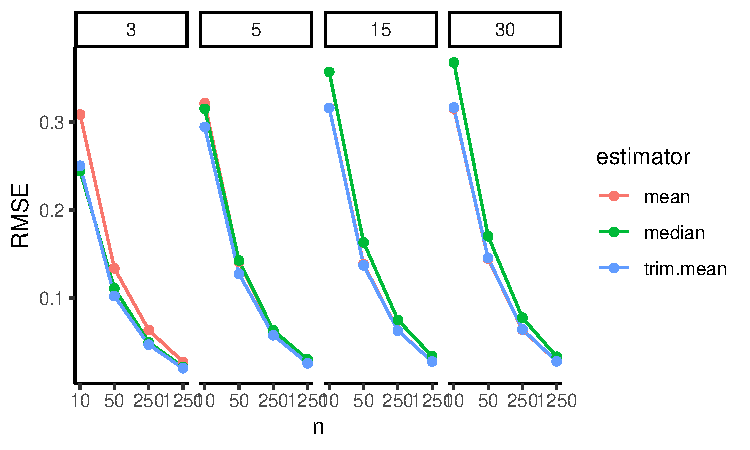
\includegraphics[width=0.75\linewidth]{Designing-Simulations-in-R_files/figure-latex/unnamed-chunk-179-1} \end{center}

\section{Improving the visualization of the results}\label{improving-the-visualization-of-the-results}

The above doesn't show differences clearly because all the RMSE goes to zero.
It helps to log our outcome, or otherwise rescale. The logging version shows
differences are relatively constant given changing sample size.

\begin{Shaded}
\begin{Highlighting}[]
\FunctionTok{ggplot}\NormalTok{( results, }\FunctionTok{aes}\NormalTok{(}\AttributeTok{x=}\NormalTok{n, }\AttributeTok{y=}\NormalTok{RMSE, }\AttributeTok{col=}\NormalTok{estimator) ) }\SpecialCharTok{+}
    \FunctionTok{facet\_wrap}\NormalTok{( }\SpecialCharTok{\textasciitilde{}}\NormalTok{ df, }\AttributeTok{nrow=}\DecValTok{1}\NormalTok{ ) }\SpecialCharTok{+}
    \FunctionTok{geom\_line}\NormalTok{() }\SpecialCharTok{+} \FunctionTok{geom\_point}\NormalTok{() }\SpecialCharTok{+}
    \FunctionTok{scale\_x\_log10}\NormalTok{( }\AttributeTok{breaks=}\NormalTok{ns ) }\SpecialCharTok{+}
    \FunctionTok{scale\_y\_log10}\NormalTok{()}
\end{Highlighting}
\end{Shaded}

\begin{center}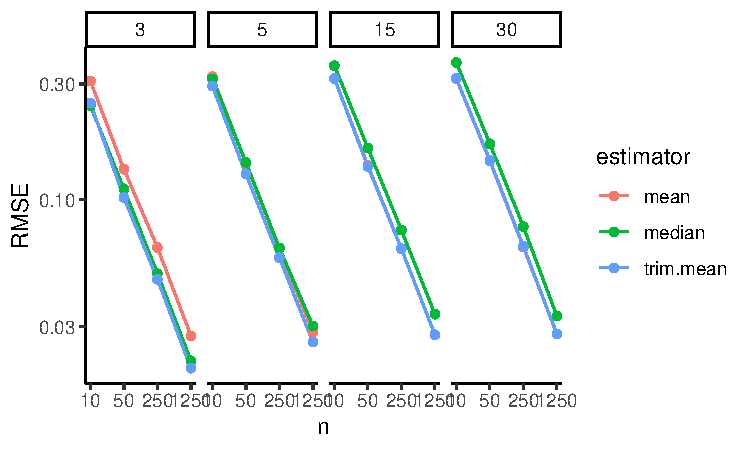
\includegraphics[width=0.75\linewidth]{Designing-Simulations-in-R_files/figure-latex/unnamed-chunk-180-1} \end{center}

Better is to rescale using our knowledge of standard errors. If we scale by
the square root of sample size, we should get horizontal lines. We now
clearly see the trends.

\begin{Shaded}
\begin{Highlighting}[]
\NormalTok{results }\OtherTok{\textless{}{-}} \FunctionTok{mutate}\NormalTok{( results, }\AttributeTok{scaleRMSE =}\NormalTok{ RMSE }\SpecialCharTok{*} \FunctionTok{sqrt}\NormalTok{(n) )}
\end{Highlighting}
\end{Shaded}

\begin{Shaded}
\begin{Highlighting}[]
\FunctionTok{ggplot}\NormalTok{( results, }\FunctionTok{aes}\NormalTok{(}\AttributeTok{x=}\NormalTok{n, }\AttributeTok{y=}\NormalTok{scaleRMSE, }\AttributeTok{col=}\NormalTok{estimator) ) }\SpecialCharTok{+}
    \FunctionTok{facet\_wrap}\NormalTok{( }\SpecialCharTok{\textasciitilde{}}\NormalTok{ df, }\AttributeTok{nrow=}\DecValTok{1}\NormalTok{) }\SpecialCharTok{+}
    \FunctionTok{geom\_line}\NormalTok{() }\SpecialCharTok{+} \FunctionTok{geom\_point}\NormalTok{() }\SpecialCharTok{+}
    \FunctionTok{scale\_x\_log10}\NormalTok{( }\AttributeTok{breaks=}\NormalTok{ns )}
\end{Highlighting}
\end{Shaded}

\begin{center}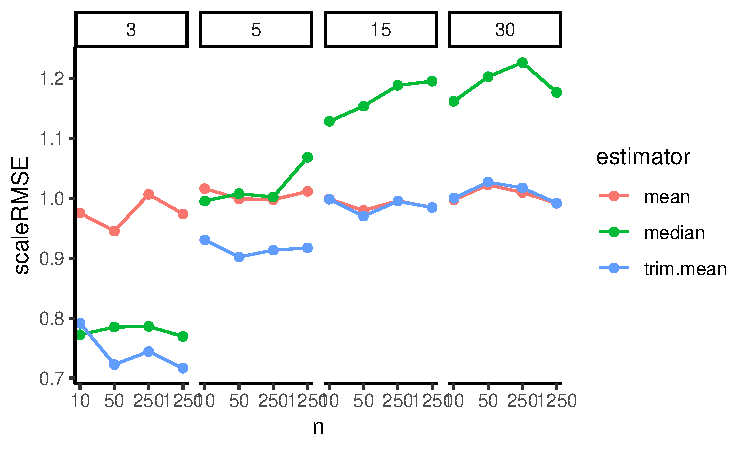
\includegraphics[width=0.75\linewidth]{Designing-Simulations-in-R_files/figure-latex/unnamed-chunk-182-1} \end{center}

Overall, we see the scaled error of the mean it is stable across the
different distributions. The trimmed mean is a real advantage when the
degrees of freedom are small. We are cropping outliers that destabilize our
estimate which leads to great wins. As the distribution grows more normal,
this is no longer an advantage and we get closer to the mean in terms of
performance. Here we are penalized slightly bye having dropped 10\% of our
data, so the standard errors will be slightly larger.

The median is not able to take advantage of the nuances of a data set because
it is entirely determined by the middle value. When outliers cause real
concern, this cost is minimal. When outliers are not a concern, the median is
just worse.

Overall, the trimmed mean seems an excellent choice: in the presence of
outliers it is far more stable than the mean, and when there are no outliers
the cost of using it is small.

In terms of thinking about designing simulation studies, we see clear
visual displays of simulation results can tell very clear stories. Eschew
complicated tables with lots of numbers.

\section{Extension: The Bias-variance tradeoff}\label{extension-the-bias-variance-tradeoff}

We can use the above simulation to examine these same estimators when we the
median is not the same as the mean. Say we want the mean of a distribution,
but have systematic outliers. If we just use the median, or trimmed mean, we
might have bias if the outliers tend to be on one side or another. For
example, consider the exponential distribution:

\begin{Shaded}
\begin{Highlighting}[]
\NormalTok{nums }\OtherTok{=} \FunctionTok{rexp}\NormalTok{( }\DecValTok{100000}\NormalTok{ )}
\FunctionTok{mean}\NormalTok{( nums )}
\end{Highlighting}
\end{Shaded}

\begin{verbatim}
## [1] 1.002233
\end{verbatim}

\begin{Shaded}
\begin{Highlighting}[]
\FunctionTok{mean}\NormalTok{( nums, }\AttributeTok{trim=}\FloatTok{0.1}\NormalTok{ )}
\end{Highlighting}
\end{Shaded}

\begin{verbatim}
## [1] 0.8323088
\end{verbatim}

\begin{Shaded}
\begin{Highlighting}[]
\FunctionTok{median}\NormalTok{( nums )}
\end{Highlighting}
\end{Shaded}

\begin{verbatim}
## [1] 0.6908992
\end{verbatim}

Our trimming, etc., is \emph{biased} if we think of our goal as estimating the
mean. But if the trimmed estimators are much more stable, we might still
wish to use them. Let's find out.

Let's generate a mixture distribution, just for fun. It will have a nice
normal base with some extreme outliers. We will make sure the overall mean,
including the outliers, is always 1, however. (So our target, \(\mu\) is now 1,
not 0.)

\begin{Shaded}
\begin{Highlighting}[]
\NormalTok{gen.data.outliers }\OtherTok{=} \ControlFlowTok{function}\NormalTok{( n, }\AttributeTok{prob.outlier =} \FloatTok{0.05}\NormalTok{ ) \{}
\NormalTok{    nN }\OtherTok{=} \FunctionTok{rbinom}\NormalTok{( }\DecValTok{1}\NormalTok{, n, prob.outlier )}
\NormalTok{    nrm }\OtherTok{=} \FunctionTok{rnorm}\NormalTok{( n }\SpecialCharTok{{-}}\NormalTok{ nN, }\AttributeTok{mean=}\FloatTok{0.5}\NormalTok{, }\AttributeTok{sd=}\DecValTok{1}\NormalTok{ )}
\NormalTok{    outmean }\OtherTok{=}\NormalTok{ (}\DecValTok{1} \SpecialCharTok{{-}}\NormalTok{ (}\DecValTok{1}\SpecialCharTok{{-}}\NormalTok{prob.outlier)}\SpecialCharTok{/}\DecValTok{2}\NormalTok{) }\SpecialCharTok{/}\NormalTok{ prob.outlier}
\NormalTok{    outs }\OtherTok{=} \FunctionTok{rnorm}\NormalTok{( nN, }\AttributeTok{mean=}\NormalTok{outmean, }\AttributeTok{sd=}\DecValTok{10}\NormalTok{ )}
    \FunctionTok{c}\NormalTok{( nrm, outs )}
\NormalTok{\}}
\end{Highlighting}
\end{Shaded}

Let's look at our distribution

\begin{Shaded}
\begin{Highlighting}[]
\NormalTok{Y }\OtherTok{=} \FunctionTok{gen.data.outliers}\NormalTok{( }\DecValTok{10000000}\NormalTok{, }\AttributeTok{prob.outlier =} \FloatTok{0.05}\NormalTok{ )}
\FunctionTok{mean}\NormalTok{( Y )}
\end{Highlighting}
\end{Shaded}

\begin{verbatim}
## [1] 1.000522
\end{verbatim}

\begin{Shaded}
\begin{Highlighting}[]
\FunctionTok{sd}\NormalTok{( Y )}
\end{Highlighting}
\end{Shaded}

\begin{verbatim}
## [1] 3.273068
\end{verbatim}

\begin{Shaded}
\begin{Highlighting}[]
\FunctionTok{hist}\NormalTok{( Y, }\AttributeTok{breaks=}\DecValTok{30}\NormalTok{, }\AttributeTok{col=}\StringTok{"grey"}\NormalTok{, }\AttributeTok{prob=}\ConstantTok{TRUE}\NormalTok{ )}
\end{Highlighting}
\end{Shaded}

\begin{center}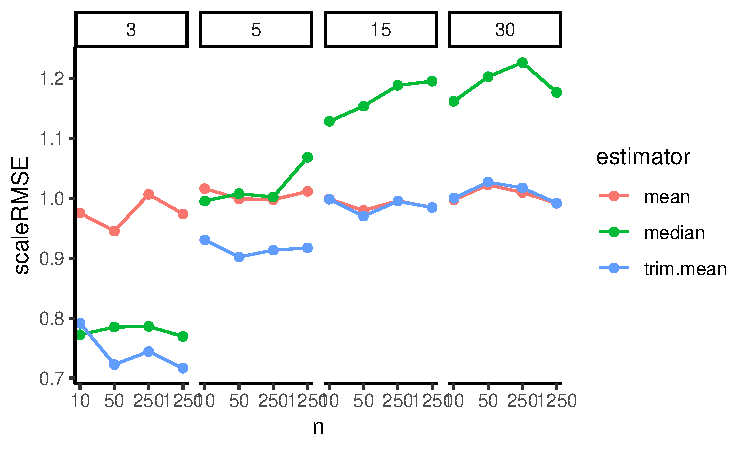
\includegraphics[width=0.75\linewidth]{Designing-Simulations-in-R_files/figure-latex/unnamed-chunk-185-1} \end{center}

We steal the code from above, modifying it slightly for our new function and
changing our target parameter from 0 to 1:

\begin{Shaded}
\begin{Highlighting}[]
\NormalTok{run.simulation.exp }\OtherTok{=} \ControlFlowTok{function}\NormalTok{( n ) \{}
\NormalTok{    raw.exps }\OtherTok{\textless{}{-}} \FunctionTok{replicate}\NormalTok{( }\DecValTok{1000}\NormalTok{, \{}
\NormalTok{        dt }\OtherTok{=} \FunctionTok{gen.data.outliers}\NormalTok{( }\AttributeTok{n=}\NormalTok{n )}
        \FunctionTok{analyze.data}\NormalTok{( dt )}
\NormalTok{    \}, }\AttributeTok{simplify =} \ConstantTok{FALSE}\NormalTok{ )}
\NormalTok{    raw.exps }\OtherTok{=} \FunctionTok{bind\_rows}\NormalTok{( raw.exps, }\AttributeTok{.id =} \StringTok{"runID"}\NormalTok{ )}

\NormalTok{    rs }\OtherTok{\textless{}{-}}\NormalTok{ raw.exps }\SpecialCharTok{\%\textgreater{}\%}
        \FunctionTok{group\_by}\NormalTok{( estimator ) }\SpecialCharTok{\%\textgreater{}\%}
        \FunctionTok{summarise}\NormalTok{( }\AttributeTok{qual =} \FunctionTok{estimator.quality}\NormalTok{( estimate, }\AttributeTok{mu =} \DecValTok{1}\NormalTok{ ) ) }\SpecialCharTok{\%\textgreater{}\%}
\NormalTok{        tidyr}\SpecialCharTok{::}\FunctionTok{unpack}\NormalTok{( }\AttributeTok{cols =} \FunctionTok{c}\NormalTok{( qual ) )}

\NormalTok{    rs}
\NormalTok{\}}

\NormalTok{res }\OtherTok{=} \FunctionTok{run.simulation.exp}\NormalTok{( }\DecValTok{100}\NormalTok{ )}
\NormalTok{res}
\end{Highlighting}
\end{Shaded}

\begin{verbatim}
## # A tibble: 3 x 4
##   estimator  RMSE     bias    SE
##   <chr>     <dbl>    <dbl> <dbl>
## 1 mean      0.326 -0.00208 0.326
## 2 median    0.475 -0.457   0.130
## 3 trim.mean 0.455 -0.440   0.115
\end{verbatim}

And for our experiment we vary the sample size

\begin{Shaded}
\begin{Highlighting}[]
\NormalTok{ns }\OtherTok{=} \FunctionTok{c}\NormalTok{( }\DecValTok{10}\NormalTok{, }\DecValTok{20}\NormalTok{, }\DecValTok{40}\NormalTok{, }\DecValTok{80}\NormalTok{, }\DecValTok{160}\NormalTok{, }\DecValTok{320}\NormalTok{ )}
\NormalTok{lvls }\OtherTok{=} \FunctionTok{tibble}\NormalTok{( }\AttributeTok{n=}\NormalTok{ns )}
\end{Highlighting}
\end{Shaded}

\begin{Shaded}
\begin{Highlighting}[]
\NormalTok{results }\OtherTok{\textless{}{-}}\NormalTok{ lvls }\SpecialCharTok{\%\textgreater{}\%} 
  \FunctionTok{mutate}\NormalTok{( }\AttributeTok{results =} \FunctionTok{pmap}\NormalTok{( lvls, run.simulation.exp ) ) }\SpecialCharTok{\%\textgreater{}\%} 
  \FunctionTok{unnest}\NormalTok{( }\AttributeTok{cols =} \FunctionTok{c}\NormalTok{(results) )}
\FunctionTok{head}\NormalTok{( results )}
\end{Highlighting}
\end{Shaded}

\begin{verbatim}
## # A tibble: 6 x 5
##       n estimator  RMSE      bias    SE
##   <dbl> <chr>     <dbl>     <dbl> <dbl>
## 1    10 mean      1.04  -0.0265   1.04 
## 2    10 median    0.593 -0.454    0.381
## 3    10 trim.mean 0.655 -0.381    0.533
## 4    20 mean      0.740 -0.000791 0.740
## 5    20 median    0.536 -0.454    0.285
## 6    20 trim.mean 0.518 -0.410    0.317
\end{verbatim}

Here we are going to plot multiple outcomes. Often with the simulation study
we are interested in different measures of performance. For us, we want to
know the standard error, bias, and overall error (RMSE). To plot this we
first gather our outcomes to make a long form dataframe of results:

\begin{Shaded}
\begin{Highlighting}[]
\NormalTok{res2 }\OtherTok{=} \FunctionTok{gather}\NormalTok{( results, RMSE, bias, SE, }\AttributeTok{key=}\StringTok{"Measure"}\NormalTok{,}\AttributeTok{value=}\StringTok{"value"}\NormalTok{ )}
\NormalTok{res2 }\OtherTok{=} \FunctionTok{mutate}\NormalTok{( res2, }\AttributeTok{Measure =} \FunctionTok{factor}\NormalTok{( Measure, }\AttributeTok{levels=}\FunctionTok{c}\NormalTok{(}\StringTok{"SE"}\NormalTok{,}\StringTok{"bias"}\NormalTok{,}\StringTok{"RMSE"}\NormalTok{ )))}
\end{Highlighting}
\end{Shaded}

And then we plot, making a facet for each outcome of interest:

\begin{Shaded}
\begin{Highlighting}[]
\FunctionTok{ggplot}\NormalTok{( res2, }\FunctionTok{aes}\NormalTok{(}\AttributeTok{x=}\NormalTok{n, }\AttributeTok{y=}\NormalTok{value, }\AttributeTok{col=}\NormalTok{estimator) ) }\SpecialCharTok{+}
    \FunctionTok{facet\_grid}\NormalTok{( . }\SpecialCharTok{\textasciitilde{}}\NormalTok{ Measure ) }\SpecialCharTok{+}
    \FunctionTok{geom\_hline}\NormalTok{( }\AttributeTok{yintercept=}\DecValTok{0}\NormalTok{, }\AttributeTok{col=}\StringTok{"darkgrey"}\NormalTok{ ) }\SpecialCharTok{+}
    \FunctionTok{geom\_line}\NormalTok{() }\SpecialCharTok{+} \FunctionTok{geom\_point}\NormalTok{() }\SpecialCharTok{+}
    \FunctionTok{scale\_x\_log10}\NormalTok{( }\AttributeTok{breaks=}\NormalTok{ns ) }\SpecialCharTok{+}
    \FunctionTok{labs}\NormalTok{( }\AttributeTok{y=}\StringTok{""}\NormalTok{ )}
\end{Highlighting}
\end{Shaded}

\begin{center}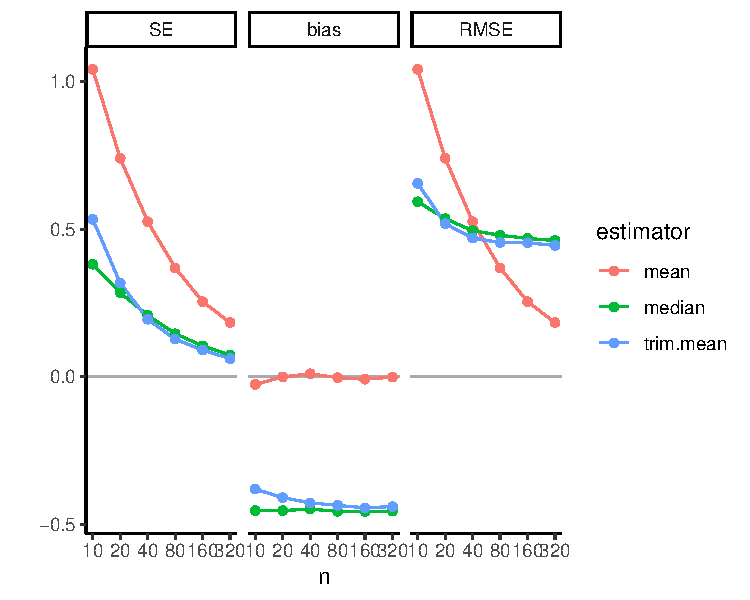
\includegraphics[width=0.75\linewidth]{Designing-Simulations-in-R_files/figure-latex/unnamed-chunk-189-1} \end{center}

We see how different estimators have different biases and different
uncertainties. The bias is negative for our trimmed estimators because we
are losing the big outliers above and so getting answers that are too low.

The RMSE captures the trade-off in terms of what estimator gives the lowest
overall \emph{error}. For this distribution, the mean wins as the sample size
increases because the bias basically stays the same and the SE drops. But
for smaller samples the trimming is superior. The median (essentially
trimming 50\% above and below) is overkill and has too much negative bias.

From a simulation study point of view, notice how we are looking at three
different qualities of our estimators. Some people really care about bias,
some care about RMSE. By presenting all results we are transparent about how
the different estimators operate.

Next steps would be to also examine the associated estimated standard errors
for the estimators, seeing if these estimates of estimator uncertainty are
good or poor. This leads to investigation of coverage rates and similar.

\chapter{Presentation of simulation results}\label{presentation-of-simulation-results}

Last chapter, we started to investigate how to present a multifactor experiment.
In this chapter, we talk about some principles behind the choices one might make in generating final reports of a simulation.
There are three primary approaches to the analysis and presentation of simulation results:

\begin{enumerate}
\def\labelenumi{\arabic{enumi}.}
\tightlist
\item
  Tabulation
\item
  Visualization
\item
  Modeling
\end{enumerate}

There are generally two primary goals for your results:

\begin{itemize}
\tightlist
\item
  Understand the effects of all of the factors manipulated in the simulation.
\item
  Develop evidence that addresses your research questions.
\end{itemize}

For your final write-up, you will not want to present everything.
A wall of numbers and observations will serve to pummel the reader, rather than inform them; readers rarely enjoy being pummeled, and the solution is quite often to skim such material while feeling hurt and betayed.
Instead, you should present selected results that clearly illustrate the main findings from the study and anything unusual/anomolous.
This will typically be with a few well-chosen figues.
Then, in the text of your write-up, you might include examples that make specific numerical comparisons.
Do not include too many of theses, and be sure to say why the numerical comparisons you include are important.
Finally, have supplementary materials that contain further detail such as additional figures and analysis, and complete simulation results.

If you want to be a moral person worthy of the awards of Heaven, you should also provide reproducible code so others could, if so desired, rerun the simulation and conduct the analysis themselves.
This last part provides a great legitimacy bump to your work: even if no one touches your code, knowing that they could builds confidence.
People naturally think, ``if that researcher is so willing to let me see what they actually did, then they must be fairly confident it does not contain too many horrendous mistakes and it is probably right.''

We briefly walk through the three modes of engaging with one's simulation results, with a few examples taken from the literature.

\section{Tabulation}\label{tabulation}

Traditionally, simulation study results are presented in big tables.
We think this doesn't really make the take-aways of a simulation readily apparent.
Perhaps tables are fine if\ldots{}
- they involve only a few numbers, and a few targeted comparisons
- it is important to report \emph{exact} values for some quantities

Unfortunately, simulations usually produce lots of numbers, and involve making lots of comparisons.
You are going to want to show, for example, the relative performance of alternative estimators, or the performance of your estimators under different conditions for the data-generating model.
This means a lot of rows, and a lot of dimensions.
Tables can do two dimensions; when you try to cram more than that into a table, no one is particularly well served.

Furthermore, in simulation, exact values for your bias/RMSE/type-I error, or whatever, are not usually of interest. And in fact, we rarely have them due to Monte Carlo simulation error.
The tables provide a false sense of security, unless you include uncertainty, which clutters your table even further.

Tables and simulations do not particularly well mix.
In particular, if you are ever tempted into putting your table in landscape mode to get it to fit on the page, think again.
It is often more useful and insightful to present results in graphs (Gelman, Pasarica, \& Dodhia, 2002).

So, onwards.

\section{Visualization}\label{visualization}

Visualization should nearly always be the first step in analyzing simulation results.

This often requires creating a \emph{BUNCH} of graphs to look at different aspects of the data.

Helpful tools/concepts:

\begin{itemize}
\tightlist
\item
  Boxplots are often useful for depicting range and central tendency across many combinations of parameter values.
\item
  Use color, shape, and line type to encode different factors
\item
  Small multiples (faceting) can then encode further factors (e.g., varying sample size)
\end{itemize}

We next present a series of visualizations taken from our published work, illustrating some different themes behind visualization that we believe are important.

\subsection{Example 1: Biserial correlation estimation}\label{example-1-biserial-correlation-estimation}

Our first example shows the bias of a biserial correlation estimate from an extreme groups design.
This simulation was a \(96 \times 2 \times 5 \times 5\) factorial design (true correlation for a range of values, cut-off type, cut-off percentile, and sample size).
The correlation, with 96 levels, forms the \(x\)-axis, giving us nice performance curves.
We use line type for the sample size, allowing us to easily see how bias collapses as sample size increases.
Finally, the facet grid gives our final factors of cut-off type and cut-off percentile.
All our factors, and nearly 5000 explored simulation scenarios, are visible in a single plot.

\begin{verbatim}
## `geom_smooth()` using formula = 'y ~ x'
\end{verbatim}

\begin{center}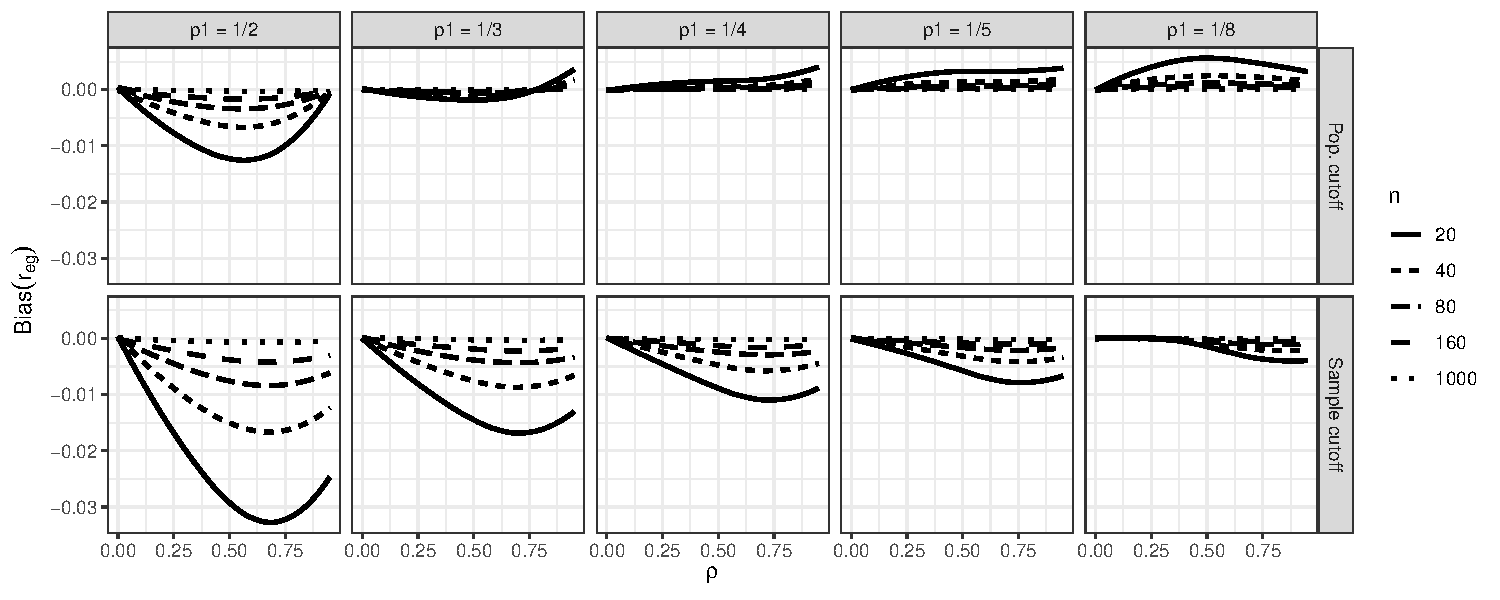
\includegraphics[width=0.75\linewidth]{Designing-Simulations-in-R_files/figure-latex/unnamed-chunk-191-1} \end{center}

Source: Pustejovsky, J. E. (2014). Converting from d to r to z when the design uses extreme groups, dichotomization, or experimental control. Psychological Methods, 19(1), 92-112.

Note that in our figure, we have smoothed the lines with respect to \texttt{rho} using \texttt{geom\_smooth()}.
This is a nice tool for taking some of the simulation jitter out of an analysis to show overall trends more directly.

\subsection{Example 2: Variance estimation and Meta-regression}\label{example-2-variance-estimation-and-meta-regression}

\begin{itemize}
\tightlist
\item
  Type-I error rates of small-sample corrected F-tests based on cluster-robust variance estimation in meta-regression
\item
  Comparison of 5 different small-sample corrections
\item
  Complex experimental design, varying

  \begin{itemize}
  \tightlist
  \item
    sample size (\(m\))
  \item
    dimension of hypothesis (\(q\))
  \item
    covariates tested
  \item
    degree of model mis-specification
  \end{itemize}
\end{itemize}

\begin{center}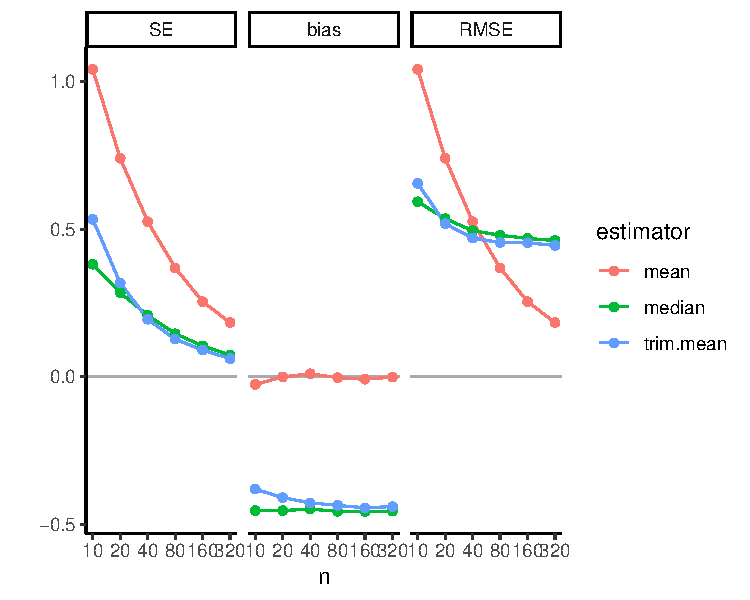
\includegraphics[width=0.75\linewidth]{Designing-Simulations-in-R_files/figure-latex/unnamed-chunk-192-1} \end{center}

Source: Tipton, E., \& Pustejovsky, J. E. (2015). Small-sample adjustments for tests of moderators and model fit using robust variance estimation in meta-regression. \emph{Journal of Educational and Behavioral Statistics, 40}(6), 604-634.

\subsection{Example: Heat maps of coverage}\label{example-heat-maps-of-coverage}

The visualization below shows the coverage of parametric bootstrap confidence intervals for momentary time sampling data
In this simulation study the authors were comparing maximum likelihood estimators to posterior mode (penalized likelihood) estimators of prevalence.
We have a 2-dimensional parameter space of prevalence (19 levels) by incidence (10 levels).
We also have 15 levels of sample size.

One option here is to use a heat map, showing the combinations of prevelance and incidence as a grid for each sample size level.
We break coverage into ranges of interest, with green being ``good'' (near 95\%) and yellow being ``close'' (92.5\% or above).
For this to work, we need our MCSE to be small enough that our coverage is estimated precisely enough to show structure.

\begin{verbatim}
## Warning: `qplot()` was deprecated in ggplot2 3.4.0.
## This warning is displayed once every 8 hours.
## Call `lifecycle::last_lifecycle_warnings()` to
## see where this warning was generated.
\end{verbatim}

\begin{center}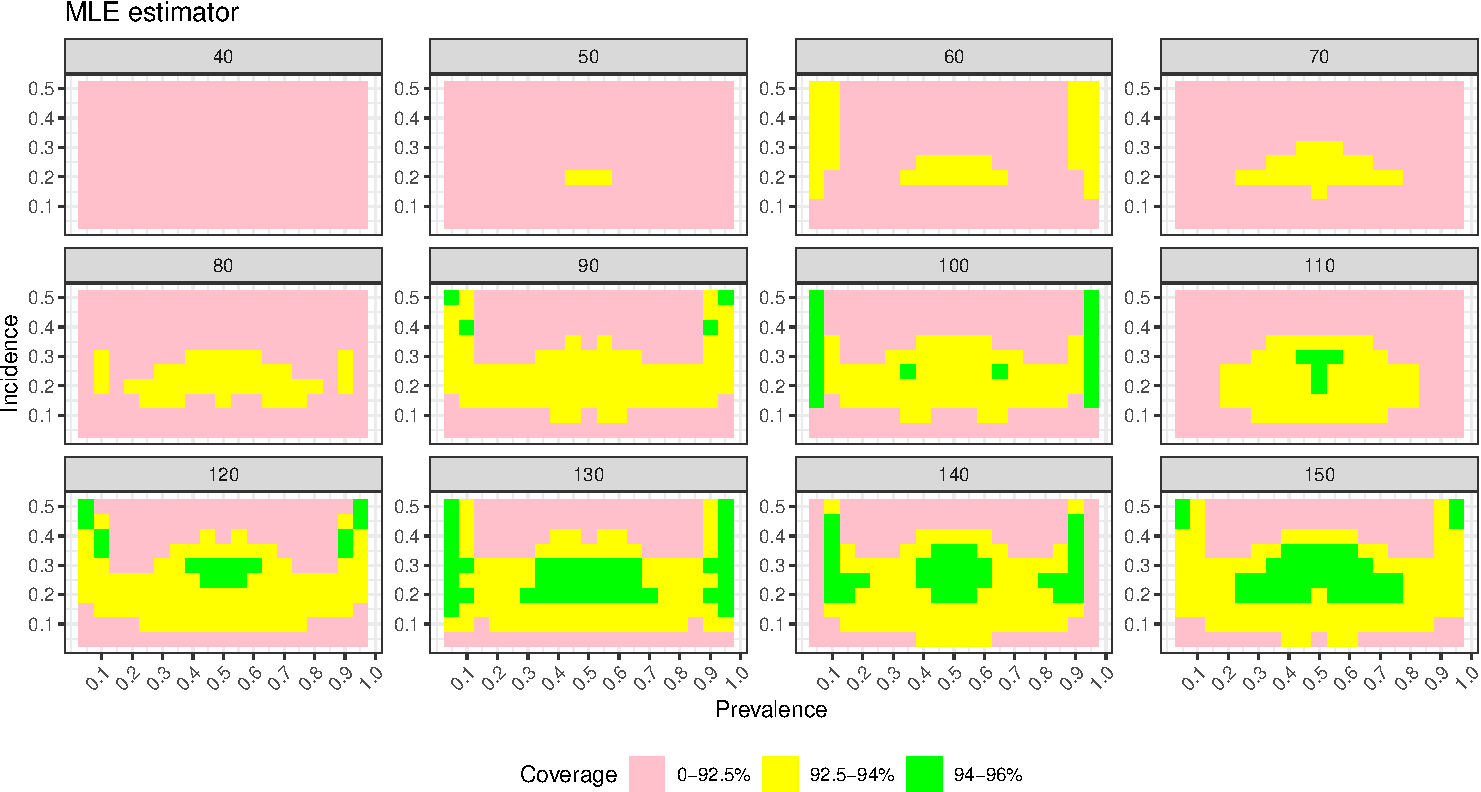
\includegraphics[width=0.75\linewidth]{Designing-Simulations-in-R_files/figure-latex/swan_example_setup-1} \end{center}

\begin{center}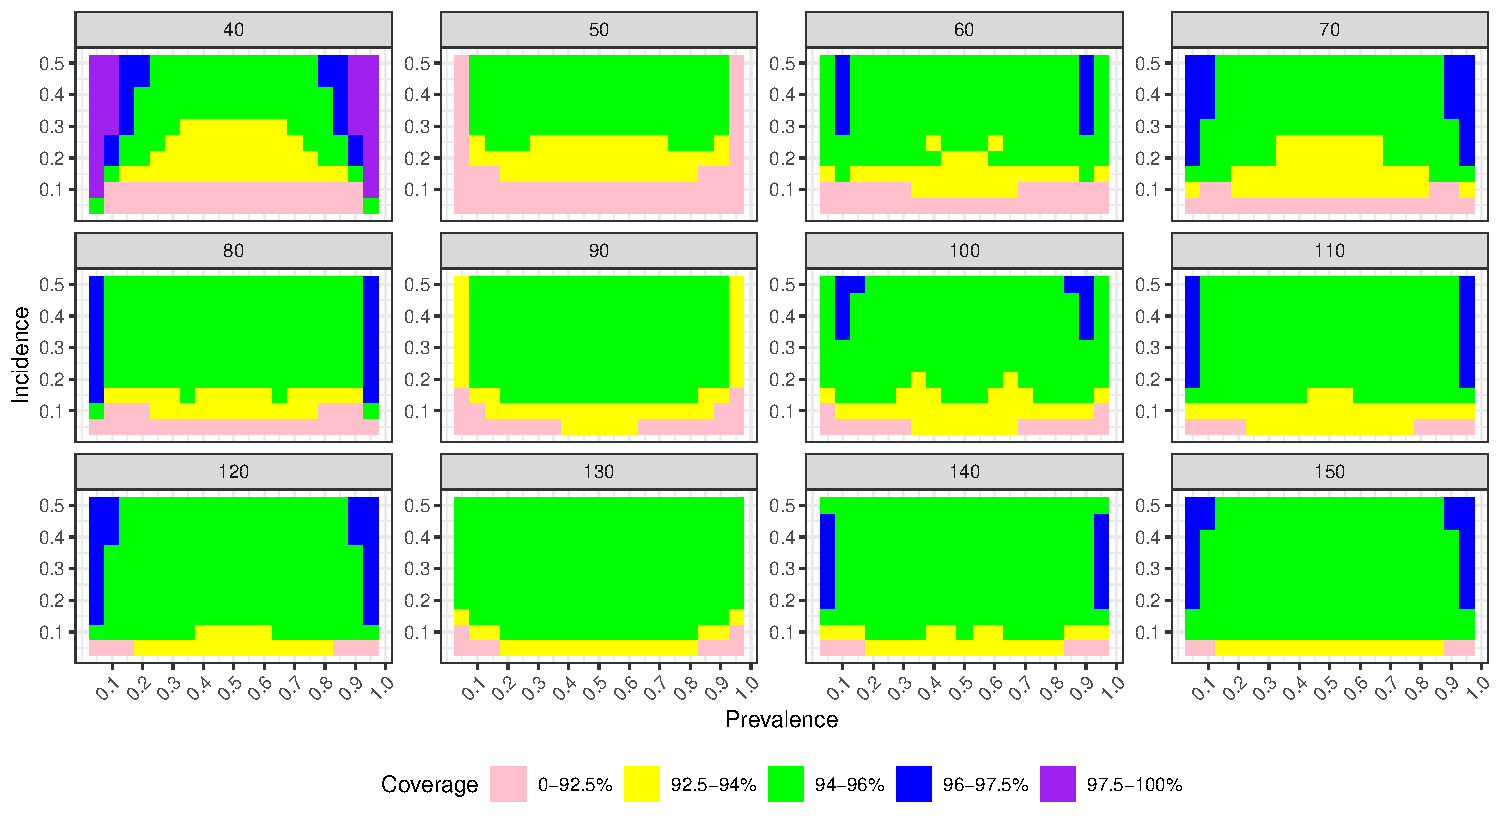
\includegraphics[width=0.75\linewidth]{Designing-Simulations-in-R_files/figure-latex/unnamed-chunk-193-1} \end{center}

To see this plot IRL, see Pustejovsky, J. E., \& Swan, D. M. (2015). Four methods for analyzing partial interval recording data, with application to single-case research. \emph{Multivariate Behavioral Research, 50}(3), 365-380.

\section{Modeling}\label{modeling}

Simulations are designed experiments, often with a full factorial structure.
We can therefore leverage classic means for analyzing such full factorial experiment.
In particular, we in effect model how a performance measure varies as a function of the different experimental factors.
We can use regression or other modeling to do this.

First, in the language of a full factor experiment, we might be interested in the ``main effects'' or ``interaction effects.''
A main effect is whether, averaging across the other factors in our experiment, a factor of interest systematically impacts our peformance measure.
When we look at a main effect, the other factors help ensure our main effect is generalizable: if we see a trend when we average over the other varying aspects, then we can state that for a host of simulation contexts, grouped by levels of our main effect, we see a trend.

For example, consider the Bias of biserial correlation estimate from an extreme groups design example from above.
Visually, we see that most factors appear to matter for bias, but we might want to get a sense of how much.
In particular, does the the population vs sample cutoff option matter, on average, for bias?

\begin{Shaded}
\begin{Highlighting}[]
\FunctionTok{options}\NormalTok{(}\AttributeTok{scipen =} \DecValTok{5}\NormalTok{)}
\NormalTok{mod }\OtherTok{=} \FunctionTok{lm}\NormalTok{( bias }\SpecialCharTok{\textasciitilde{}}\NormalTok{ fixed }\SpecialCharTok{+}\NormalTok{ rho }\SpecialCharTok{+} \FunctionTok{I}\NormalTok{(rho}\SpecialCharTok{\^{}}\DecValTok{2}\NormalTok{) }\SpecialCharTok{+}\NormalTok{ p1 }\SpecialCharTok{+}\NormalTok{ n, }\AttributeTok{data =}\NormalTok{ r\_F)}
\FunctionTok{summary}\NormalTok{(mod, }\AttributeTok{digits=}\DecValTok{2}\NormalTok{)}
\end{Highlighting}
\end{Shaded}

\begin{verbatim}
## 
## Call:
## lm(formula = bias ~ fixed + rho + I(rho^2) + p1 + n, data = r_F)
## 
## Residuals:
##        Min         1Q     Median         3Q 
## -0.0215935 -0.0013608  0.0003823  0.0015677 
##        Max 
##  0.0081802 
## 
## Coefficients:
##                       Estimate  Std. Error
## (Intercept)         0.00218473  0.00015107
## fixedSample cutoff -0.00363520  0.00009733
## rho                -0.00942338  0.00069578
## I(rho^2)            0.00720857  0.00070868
## p1.L                0.00461700  0.00010882
## p1.Q               -0.00160546  0.00010882
## p1.C                0.00081464  0.00010882
## p1^4               -0.00011190  0.00010882
## n.L                 0.00362949  0.00010882
## n.Q                -0.00103981  0.00010882
## n.C                 0.00027941  0.00010882
## n^4                 0.00001976  0.00010882
##                    t value Pr(>|t|)    
## (Intercept)         14.462  < 2e-16 ***
## fixedSample cutoff -37.347  < 2e-16 ***
## rho                -13.544  < 2e-16 ***
## I(rho^2)            10.172  < 2e-16 ***
## p1.L                42.426  < 2e-16 ***
## p1.Q               -14.753  < 2e-16 ***
## p1.C                 7.486 8.41e-14 ***
## p1^4                -1.028   0.3039    
## n.L                 33.352  < 2e-16 ***
## n.Q                 -9.555  < 2e-16 ***
## n.C                  2.568   0.0103 *  
## n^4                  0.182   0.8559    
## ---
## Signif. codes:  
## 0 '***' 0.001 '**' 0.01 '*' 0.05 '.' 0.1 ' ' 1
## 
## Residual standard error: 0.003372 on 4788 degrees of freedom
## Multiple R-squared:  0.5107, Adjusted R-squared:  0.5096 
## F-statistic: 454.4 on 11 and 4788 DF,  p-value: < 2.2e-16
\end{verbatim}

The above printout gives main effects for each factor, averaged across other factors.
It is automatically generating linear, quadradic, cubic and fourth order contrasts for the ordered factors of p1 and n.
We see that, across other contexts, the sample cutoff is around 0.004 lower than population.

We next discuss two additional tools:

\begin{quote}
\begin{itemize}
\tightlist
\item
  ANOVA can be useful for understanding major sources of variation in simulation results (e.g., identifying which factors have negligible/minor influence on the bias of an estimator).
\item
  Smoothing (e.g., local linear regression) over continuous factors
\end{itemize}
\end{quote}

\begin{Shaded}
\begin{Highlighting}[]
\NormalTok{anova\_table }\OtherTok{\textless{}{-}} \FunctionTok{aov}\NormalTok{(bias }\SpecialCharTok{\textasciitilde{}}\NormalTok{ rho }\SpecialCharTok{*}\NormalTok{ p1 }\SpecialCharTok{*}\NormalTok{ fixed }\SpecialCharTok{*}\NormalTok{ n, }\AttributeTok{data =}\NormalTok{ r\_F)}
\FunctionTok{summary}\NormalTok{(anova\_table)}
\end{Highlighting}
\end{Shaded}

\begin{verbatim}
##                  Df   Sum Sq  Mean Sq  F value
## rho               1 0.002444 0.002444  1673.25
## p1                4 0.023588 0.005897  4036.41
## fixed             1 0.015858 0.015858 10854.52
## n                 4 0.013760 0.003440  2354.60
## rho:p1            4 0.001722 0.000431   294.71
## rho:fixed         1 0.003440 0.003440  2354.69
## p1:fixed          4 0.001683 0.000421   287.98
## rho:n             4 0.002000 0.000500   342.31
## p1:n             16 0.019810 0.001238   847.51
## fixed:n           4 0.013359 0.003340  2285.97
## rho:p1:fixed      4 0.000473 0.000118    80.87
## rho:p1:n         16 0.001470 0.000092    62.91
## rho:fixed:n       4 0.002929 0.000732   501.23
## p1:fixed:n       16 0.001429 0.000089    61.12
## rho:p1:fixed:n   16 0.000429 0.000027    18.36
## Residuals      4700 0.006866 0.000001         
##                Pr(>F)    
## rho            <2e-16 ***
## p1             <2e-16 ***
## fixed          <2e-16 ***
## n              <2e-16 ***
## rho:p1         <2e-16 ***
## rho:fixed      <2e-16 ***
## p1:fixed       <2e-16 ***
## rho:n          <2e-16 ***
## p1:n           <2e-16 ***
## fixed:n        <2e-16 ***
## rho:p1:fixed   <2e-16 ***
## rho:p1:n       <2e-16 ***
## rho:fixed:n    <2e-16 ***
## p1:fixed:n     <2e-16 ***
## rho:p1:fixed:n <2e-16 ***
## Residuals                
## ---
## Signif. codes:  
## 0 '***' 0.001 '**' 0.01 '*' 0.05 '.' 0.1 ' ' 1
\end{verbatim}

\begin{Shaded}
\begin{Highlighting}[]
\FunctionTok{library}\NormalTok{(lsr)}
\FunctionTok{etaSquared}\NormalTok{(anova\_table)}
\end{Highlighting}
\end{Shaded}

\begin{verbatim}
##                     eta.sq eta.sq.part
## rho            0.021971037  0.26254289
## p1             0.212004203  0.77453319
## fixed          0.142527898  0.69783705
## n              0.123670355  0.66710072
## rho:p1         0.015479114  0.20052330
## rho:fixed      0.030918819  0.33377652
## p1:fixed       0.015125570  0.19684488
## rho:n          0.017979185  0.22560369
## p1:n           0.178055588  0.74260975
## fixed:n        0.120065971  0.66049991
## rho:p1:fixed   0.004247472  0.06439275
## rho:p1:n       0.013216569  0.17638308
## rho:fixed:n    0.026326074  0.29902214
## p1:fixed:n     0.012839790  0.17222072
## rho:p1:fixed:n 0.003857877  0.05883389
\end{verbatim}

\cmntM{Perhaps we need an example where some things don't matter?  We need to discuss what one learns from this table.}

\part{Common Challenges with Large-Scale Simulations}\label{part-common-challenges-with-large-scale-simulations}

\chapter{Ensuring reproducibility}\label{sec-reproducability}

In the prior section we built a simulation driver.
Because this function involves generating random numbers, re-running it with the exact same input parameters will still produce different results:

\begin{Shaded}
\begin{Highlighting}[]
\FunctionTok{run\_alpha\_sim}\NormalTok{(}\AttributeTok{iterations =} \DecValTok{10}\NormalTok{, }\AttributeTok{n =} \DecValTok{50}\NormalTok{, }\AttributeTok{p =} \DecValTok{6}\NormalTok{, }\AttributeTok{alpha =} \FloatTok{0.73}\NormalTok{, }\AttributeTok{df =} \DecValTok{5}\NormalTok{)}
\end{Highlighting}
\end{Shaded}

\begin{verbatim}
##         criterion         est        MCSE
## 1      alpha bias -0.03322927 0.031758861
## 2      alpha RMSE  0.10090497 0.008743501
## 3 V relative bias  0.48077615 0.114109836
## 4        coverage  0.80000000 0.068920244
\end{verbatim}

\begin{Shaded}
\begin{Highlighting}[]
\FunctionTok{run\_alpha\_sim}\NormalTok{(}\AttributeTok{iterations =} \DecValTok{10}\NormalTok{, }\AttributeTok{n =} \DecValTok{50}\NormalTok{, }\AttributeTok{p =} \DecValTok{6}\NormalTok{, }\AttributeTok{alpha =} \FloatTok{0.73}\NormalTok{, }\AttributeTok{df =} \DecValTok{5}\NormalTok{)}
\end{Highlighting}
\end{Shaded}

\begin{verbatim}
##         criterion         est        MCSE
## 1      alpha bias 0.004056121 0.015203417
## 2      alpha RMSE 0.045790250 0.002703622
## 3 V relative bias 1.511919446 0.207758767
## 4        coverage 1.000000000 0.068920244
\end{verbatim}

Of course, using a larger number of iterations will give us more precise estimates of the performance criteria. If we want to get the \emph{exact} same results, however, we have to control the random process.

This is more possible than it sounds: Monte Carlo simulations are random, but computers are not.
When we generate ``random numbers'' they actually come from a chain of mathematical equations that, given a number, will generate the next number in a deterministic sequence.
Given that number, it will generate the next, and so on.
The numbers we get back are a part of this chain of (very large) numbers that, ideally, cycles through an extremely long list of numbers in a haphazard and random looking fashion.

This is what the \texttt{seed} argument that we have glossed over before is all about.
If we set the same seed, we get the same results:

\begin{Shaded}
\begin{Highlighting}[]
\FunctionTok{run\_alpha\_sim}\NormalTok{(}\AttributeTok{iterations =} \DecValTok{10}\NormalTok{, }\AttributeTok{n =} \DecValTok{50}\NormalTok{, }\AttributeTok{p =} \DecValTok{6}\NormalTok{, }\AttributeTok{alpha =} \FloatTok{0.73}\NormalTok{, }\AttributeTok{df =} \DecValTok{5}\NormalTok{,}
              \AttributeTok{seed =} \DecValTok{6}\NormalTok{)}
\end{Highlighting}
\end{Shaded}

\begin{verbatim}
##         criterion         est       MCSE
## 1      alpha bias -0.02053560 0.02585963
## 2      alpha RMSE  0.08025083 0.01344827
## 3 V relative bias  0.64909209 1.43035647
## 4        coverage  0.90000000 0.06892024
\end{verbatim}

\begin{Shaded}
\begin{Highlighting}[]
\FunctionTok{run\_alpha\_sim}\NormalTok{(}\AttributeTok{iterations =} \DecValTok{10}\NormalTok{, }\AttributeTok{n =} \DecValTok{50}\NormalTok{, }\AttributeTok{p =} \DecValTok{6}\NormalTok{, }\AttributeTok{alpha =} \FloatTok{0.73}\NormalTok{, }\AttributeTok{df =} \DecValTok{5}\NormalTok{, }
              \AttributeTok{seed =} \DecValTok{6}\NormalTok{)}
\end{Highlighting}
\end{Shaded}

\begin{verbatim}
##         criterion         est       MCSE
## 1      alpha bias -0.02053560 0.02585963
## 2      alpha RMSE  0.08025083 0.01344827
## 3 V relative bias  0.64909209 1.43035647
## 4        coverage  0.90000000 0.06892024
\end{verbatim}

This is useful because it ensure the full reproducibility of the results. In practice, it is a good idea to always set seed values for your simulations, so that you (or someone else!) can exactly reproduce the results.
Let's look more at how this works.

\section{Seeds and pseudo-random number generators}\label{seeds-and-pseudo-random-number-generators}

In R, we can start a sequence of \textbf{deterministic} but \textbf{random-seeming} numbers by setting a ``seed''.
This means all the random numbers that come after it will be the same.

Compare this:

\begin{Shaded}
\begin{Highlighting}[]
\FunctionTok{rchisq}\NormalTok{(}\DecValTok{3}\NormalTok{, }\AttributeTok{df =} \DecValTok{5}\NormalTok{)}
\end{Highlighting}
\end{Shaded}

\begin{verbatim}
## [1] 1.193539 5.338936 6.294274
\end{verbatim}

\begin{Shaded}
\begin{Highlighting}[]
\FunctionTok{rchisq}\NormalTok{(}\DecValTok{3}\NormalTok{, }\AttributeTok{df =} \DecValTok{5}\NormalTok{)}
\end{Highlighting}
\end{Shaded}

\begin{verbatim}
## [1] 0.7189536 6.3697718 8.2913988
\end{verbatim}

To this:

\begin{Shaded}
\begin{Highlighting}[]
\FunctionTok{set.seed}\NormalTok{(}\DecValTok{20210527}\NormalTok{)}
\FunctionTok{rchisq}\NormalTok{(}\DecValTok{3}\NormalTok{, }\AttributeTok{df =} \DecValTok{5}\NormalTok{)}
\end{Highlighting}
\end{Shaded}

\begin{verbatim}
## [1] 1.643698 6.229613 3.249164
\end{verbatim}

\begin{Shaded}
\begin{Highlighting}[]
\FunctionTok{set.seed}\NormalTok{(}\DecValTok{20210527}\NormalTok{)}
\FunctionTok{rchisq}\NormalTok{(}\DecValTok{3}\NormalTok{, }\AttributeTok{df =} \DecValTok{5}\NormalTok{)}
\end{Highlighting}
\end{Shaded}

\begin{verbatim}
## [1] 1.643698 6.229613 3.249164
\end{verbatim}

By setting the seed the second time we reset our sequence of random numbers.
Similarly, to ensure reproducibility in our simulation, we will add an option to set the seed value of the random number generator.

This seed is low-level, meaning if we are generating numbers via \texttt{rnorm} or \texttt{rexp} or \texttt{rchisq}, it doesn't matter.
Each time we ask for a random number from the low-level pseudo-random number generator, it gives us the next number back.
These other functions, like \texttt{rnorm()}, etc., all call this low-level generator and than transform the number to be of the correct distribution.

\section{Including seed in our simulation driver}\label{including-seed-in-our-simulation-driver}

The easy way to ensure reproducability is to pass a seed as a parameter.
If we leave it NULL, we ignore it and just continue generating random numbers from wherever we are in the system.
If we specify a seed, however, we set it at the beginning of the scenario, and then all the numbers that follow will be in sequence.
Our code will typically look like this:

\begin{Shaded}
\begin{Highlighting}[]
\NormalTok{run\_alpha\_sim }\OtherTok{\textless{}{-}} \ControlFlowTok{function}\NormalTok{(iterations, n, p, alpha, df, }\AttributeTok{coverage =} \FloatTok{0.95}\NormalTok{, }\AttributeTok{seed =} \ConstantTok{NULL}\NormalTok{) \{}
  
  \ControlFlowTok{if}\NormalTok{ (}\SpecialCharTok{!}\FunctionTok{is.null}\NormalTok{(seed)) }\FunctionTok{set.seed}\NormalTok{(seed)}

\NormalTok{  results }\OtherTok{\textless{}{-}} 
    \FunctionTok{replicate}\NormalTok{(}\AttributeTok{n =}\NormalTok{ iterations, \{}
\NormalTok{      dat }\OtherTok{\textless{}{-}} \FunctionTok{r\_mvt\_items}\NormalTok{(}\AttributeTok{n =}\NormalTok{ n, }\AttributeTok{p =}\NormalTok{ p, }\AttributeTok{alpha =}\NormalTok{ alpha, }\AttributeTok{df =}\NormalTok{ df)}
      \FunctionTok{estimate\_alpha}\NormalTok{(dat, }\AttributeTok{coverage =}\NormalTok{ coverage)}
\NormalTok{    \}, }\AttributeTok{simplify =} \ConstantTok{FALSE}\NormalTok{) }\SpecialCharTok{\%\textgreater{}\%}
    \FunctionTok{bind\_rows}\NormalTok{()}
  
  \FunctionTok{alpha\_performance}\NormalTok{(results, }\AttributeTok{alpha =}\NormalTok{ alpha, }\AttributeTok{coverage =}\NormalTok{ coverage)}
\NormalTok{\}}
\end{Highlighting}
\end{Shaded}

Using our seed, we get identical results, as we saw in the intro, above.

\section{Reasons for setting the seed}\label{reasons-for-setting-the-seed}

Reproducibility allows us to easily check if we are running the same code that generate the results in some report.
It also helps with debugging.
For example, say we had an error that showed up one in a thousand, causing our simulation to crash sometimes.

If we set a seed, and see that it crashes, we can then go try and catch the error and repair our code, and then rerun the simulation.
If it runs clean, we know we got the error.
If we had not set the seed, we would not know if we were just getting (un) lucky, and avoiding the error by chance.

\chapter{Optimizing code (and why you often shouldn't)}\label{optimize-code}

Optimizing code is when you spend a bit more human effort to write code that will run faster on your computer.
In some cases, this can be a critical boost to running a simulation, where you inherently will be doing things a lot of times.
Cutting runtime down will always be tempting, as it allows you to run more replicates and get more precisely estimated performance measures for your simulation.

That being said, beyond a few obvious coding tricks we will discuss, one should optimize code only after you discover you need to.
Optimizing as you go usually means you will spend a lot of time wrestling with code far more complicated than it needs to be.
For example, often it is the estimation method that will take a lot of computational time, so having very fast data generation code won't help overall simulation runtimes much, as you are tweaking something that is only a small part of the overall pie, in terms of time.
Keep things simple; in general your time is more important than the computer's time.

In the next sections we will look at a few optimization efforts applied to the ANOVA example in the prior chapters.

\section{Hand-building functions}\label{hand-building-functions}

In the Welch example above, we used the system-implemented ANOVA.
An alternative approach would be to ``hand roll'' the ANOVA F statistic and test directly.
Doing so by hand can set you up to implement modified versions of these tests later on.
Also, although hand-building a method does take more work to program, it can result in a faster piece of code (this actually is the case here) which in turn can make the overall simulation faster.

Following the formulas on p.~129 of Brown and Forsythe (1974) we have (using data as generated in Chapter \ref{data-generating-processes}:

\begin{Shaded}
\begin{Highlighting}[]
\NormalTok{ANOVA\_F }\OtherTok{\textless{}{-}} \ControlFlowTok{function}\NormalTok{(sim\_data) \{}

\NormalTok{  x\_bar }\OtherTok{\textless{}{-}} \FunctionTok{with}\NormalTok{(sim\_data, }\FunctionTok{tapply}\NormalTok{(x, group, mean))}
\NormalTok{  s\_sq }\OtherTok{\textless{}{-}} \FunctionTok{with}\NormalTok{(sim\_data, }\FunctionTok{tapply}\NormalTok{(x, group, var))}
\NormalTok{  n }\OtherTok{\textless{}{-}} \FunctionTok{table}\NormalTok{(sim\_data}\SpecialCharTok{$}\NormalTok{group)}
\NormalTok{  g }\OtherTok{\textless{}{-}} \FunctionTok{length}\NormalTok{(x\_bar)}

\NormalTok{  df1 }\OtherTok{\textless{}{-}}\NormalTok{ g }\SpecialCharTok{{-}} \DecValTok{1}
\NormalTok{  df2 }\OtherTok{\textless{}{-}} \FunctionTok{sum}\NormalTok{(n) }\SpecialCharTok{{-}}\NormalTok{ g}

\NormalTok{  msbtw }\OtherTok{\textless{}{-}} \FunctionTok{sum}\NormalTok{(n }\SpecialCharTok{*}\NormalTok{ (x\_bar }\SpecialCharTok{{-}} \FunctionTok{mean}\NormalTok{(sim\_data}\SpecialCharTok{$}\NormalTok{x))}\SpecialCharTok{\^{}}\DecValTok{2}\NormalTok{) }\SpecialCharTok{/}\NormalTok{ df1}
\NormalTok{  mswn }\OtherTok{\textless{}{-}} \FunctionTok{sum}\NormalTok{((n }\SpecialCharTok{{-}} \DecValTok{1}\NormalTok{) }\SpecialCharTok{*}\NormalTok{ s\_sq) }\SpecialCharTok{/}\NormalTok{ df2}
\NormalTok{  fstat }\OtherTok{\textless{}{-}}\NormalTok{ msbtw }\SpecialCharTok{/}\NormalTok{ mswn}
\NormalTok{  pval }\OtherTok{\textless{}{-}} \FunctionTok{pf}\NormalTok{(fstat, df1, df2, }\AttributeTok{lower.tail =} \ConstantTok{FALSE}\NormalTok{)}

  \FunctionTok{return}\NormalTok{(pval)}
\NormalTok{\}}

\FunctionTok{ANOVA\_F}\NormalTok{(sim\_data)}
\end{Highlighting}
\end{Shaded}

\begin{verbatim}
## [1] 0.009208908
\end{verbatim}

To see the difference between our version and R's version, we can use an R package called \texttt{microbenchmark} to test how long the computations take for each version of the function.
The \texttt{microbenchmark} function runs each expression 100 times (by default) and tracks how long the computations take. It then summarizes the distribution of timings:

\begin{Shaded}
\begin{Highlighting}[]
\FunctionTok{library}\NormalTok{(microbenchmark)}
\NormalTok{timings }\OtherTok{\textless{}{-}} \FunctionTok{microbenchmark}\NormalTok{(}\AttributeTok{Rfunction =} \FunctionTok{ANOVA\_F\_aov}\NormalTok{(sim\_data),}
                          \AttributeTok{direct    =} \FunctionTok{ANOVA\_F}\NormalTok{(sim\_data))}
\NormalTok{timings}
\end{Highlighting}
\end{Shaded}

\begin{verbatim}
## Unit: microseconds
##       expr     min      lq     mean   median
##  Rfunction 453.901 605.451 711.6499 677.2505
##     direct 179.000 249.551 313.4281 282.7515
##        uq      max neval
##  762.7505 2080.700   100
##  317.9510 1612.401   100
\end{verbatim}

The direct function is 2.3 times faster than the built-in R function.

This result is not unusual.
Built-in R functions usually include lots of checks and error-handling, which take time to compute. These checks are crucial for messy, real-world data analysis but unnecessary with our pristine, simulated data.
Here we can skip them by doing the calculations directly.
In general, however, this is a trade-off: writing something yourself gives you a lot of chance to do something wrong, throwing off all your simulations. It might be faster, but you may pay dearly for it in terms of extra hours coding and debugging.
Optimize only if you need to!

\section{Computational efficiency versus simplicity}\label{sec_comp_efficiency}

An alternative approach to having a function that, for each call, generates a single set of data, would be to write a function that generates \emph{multiple} sets of simulated data all at once.

For example, for our ANOVA example we could specify that we want \texttt{R} replications of the study and have the function spit out a matrix with \texttt{R} columns, one for each simulated dataset:

\begin{Shaded}
\begin{Highlighting}[]
\NormalTok{generate\_data\_matrix }\OtherTok{\textless{}{-}} \ControlFlowTok{function}\NormalTok{(mu, sigma\_sq, sample\_size, R) \{}

\NormalTok{  N }\OtherTok{\textless{}{-}} \FunctionTok{sum}\NormalTok{(sample\_size) }
\NormalTok{  g }\OtherTok{\textless{}{-}} \FunctionTok{length}\NormalTok{(sample\_size) }
  
\NormalTok{  group }\OtherTok{\textless{}{-}} \FunctionTok{rep}\NormalTok{(}\DecValTok{1}\SpecialCharTok{:}\NormalTok{g, }\AttributeTok{times =}\NormalTok{ sample\_size) }
\NormalTok{  mu\_long }\OtherTok{\textless{}{-}} \FunctionTok{rep}\NormalTok{(mu, }\AttributeTok{times =}\NormalTok{ sample\_size)}
\NormalTok{  sigma\_long }\OtherTok{\textless{}{-}} \FunctionTok{rep}\NormalTok{(}\FunctionTok{sqrt}\NormalTok{(sigma\_sq), }\AttributeTok{times =}\NormalTok{ sample\_size) }

\NormalTok{  x\_mat }\OtherTok{\textless{}{-}} \FunctionTok{matrix}\NormalTok{(}\FunctionTok{rnorm}\NormalTok{(N }\SpecialCharTok{*}\NormalTok{ R, }\AttributeTok{mean =}\NormalTok{ mu\_long, }\AttributeTok{sd =}\NormalTok{ sigma\_long),}
                  \AttributeTok{nrow =}\NormalTok{ N, }\AttributeTok{ncol =}\NormalTok{ R)}
\NormalTok{  sim\_data }\OtherTok{\textless{}{-}} \FunctionTok{list}\NormalTok{(}\AttributeTok{group =}\NormalTok{ group, }\AttributeTok{x\_mat =}\NormalTok{ x\_mat)}
    
  \FunctionTok{return}\NormalTok{(sim\_data)}
\NormalTok{\}}

\FunctionTok{generate\_data\_matrix}\NormalTok{(}\AttributeTok{mu =}\NormalTok{ mu, }\AttributeTok{sigma\_sq =}\NormalTok{ sigma\_sq,}
                     \AttributeTok{sample\_size =}\NormalTok{ sample\_size, }\AttributeTok{R =} \DecValTok{4}\NormalTok{)}
\end{Highlighting}
\end{Shaded}

\begin{verbatim}
## $group
##  [1] 1 1 1 2 2 2 2 2 2 3 3 4 4 4 4
## 
## $x_mat
##             [,1]      [,2]       [,3]       [,4]
##  [1,]  2.1639323  1.646791 -0.9445957  1.2050393
##  [2,] -2.8225439  3.289125  0.8863700  3.7816431
##  [3,]  1.3419979 -3.020363  1.6196826  0.6425271
##  [4,] -0.5939495  1.184961  1.0200117  2.8301117
##  [5,]  0.1054279  3.499446  1.0267897  2.3166570
##  [6,]  4.0618127  4.340879  4.1291935 -1.0532910
##  [7,]  2.0611736  2.544518  1.3772973 -0.3861088
##  [8,]  2.2921786  2.299136  0.1706634  2.0329848
##  [9,]  2.5000308  3.686171  1.8712605  2.8557713
## [10,]  4.0966732  5.824634  6.6448117  2.6354699
## [11,]  5.9111997  3.480771  2.9453236  4.1680932
## [12,]  6.2201594  6.116809  5.8446326  6.2140816
## [13,]  5.9843999  6.488239  7.1954303  6.6280499
## [14,]  6.3928820  4.699057  5.9033074  8.8796297
## [15,]  7.9611464  7.282270  5.9095360  5.9131754
\end{verbatim}

This approach is a bit more computationally efficient because the setup calculations (getting \texttt{N}, \texttt{g}, \texttt{group}, \texttt{mu\_full}, and \texttt{sigma\_full}) only have to be done once instead of once per replication. It also makes clever use of vector recycling in the call to \texttt{rnorm()}. However, the structure of the resulting data is more complicated, which will make it more difficult to do the later estimation steps.
Furthermore, if the number of replicates \texttt{R} is large and each replication produces a large dataset, this ``all-at-once'' approach will entail generating and holding very large amounts of data in memory, which can create other performance issues.
On balance, we recommend the simpler approach of writing a function that generates a single simulated dataset per call (unless and until you have a principled reason to do otherwise).

\section{Reusing code to speed up computation}\label{reusing-code-to-speed-up-computation}

Computational and programming efficiency should usually be a secondary consideration when you are starting to design a simulation study.
It is better to produce accurate code, even if it is a bit slow, than to write code that is speedy but hard to follow (or even worse, that produces incorrect results).
All that said, there is some glaring redundancy in the two functions used for the ANOVA simulation.
Both \texttt{ANOVA\_F} and \texttt{Welch\_F} start by taking the simulated data and calculating summary statistics for each group, using the following code:

\begin{Shaded}
\begin{Highlighting}[]
\NormalTok{x\_bar }\OtherTok{\textless{}{-}} \FunctionTok{with}\NormalTok{(sim\_data, }\FunctionTok{tapply}\NormalTok{(x, group, mean))}
\NormalTok{s\_sq }\OtherTok{\textless{}{-}} \FunctionTok{with}\NormalTok{(sim\_data, }\FunctionTok{tapply}\NormalTok{(x, group, var))}
\NormalTok{n }\OtherTok{\textless{}{-}} \FunctionTok{table}\NormalTok{(sim\_data}\SpecialCharTok{$}\NormalTok{group)}
\NormalTok{g }\OtherTok{\textless{}{-}} \FunctionTok{length}\NormalTok{(x\_bar)}
\end{Highlighting}
\end{Shaded}

In the interest of not repeating ourselves, it would better to pull this code out as a separate function and then re-write the \texttt{ANOVA\_F} and \texttt{Welch\_F} functions to take the summary statistics as input. Here is a function that takes simulated data and returns a list of summary statistics:

\begin{Shaded}
\begin{Highlighting}[]
\NormalTok{summarize\_data }\OtherTok{\textless{}{-}} \ControlFlowTok{function}\NormalTok{(sim\_data) \{}
  
\NormalTok{  res }\OtherTok{\textless{}{-}}\NormalTok{ sim\_data }\SpecialCharTok{\%\textgreater{}\%} 
    \FunctionTok{group\_by}\NormalTok{( group ) }\SpecialCharTok{\%\textgreater{}\%}
    \FunctionTok{summarise}\NormalTok{( }\AttributeTok{x\_bar =} \FunctionTok{mean}\NormalTok{( x ),}
               \AttributeTok{s\_sq =} \FunctionTok{var}\NormalTok{( x ),}
               \AttributeTok{n =} \FunctionTok{n}\NormalTok{() )}
\NormalTok{  res}
\NormalTok{\}}
\end{Highlighting}
\end{Shaded}

We just packaged the code from above, and puts our results in a nice table (and thus pivoted to using tidyverse to calculate these things):

\begin{Shaded}
\begin{Highlighting}[]
\NormalTok{sim\_data }\OtherTok{=} \FunctionTok{generate\_data}\NormalTok{(}\AttributeTok{mu=}\NormalTok{mu, }\AttributeTok{sigma\_sq=}\NormalTok{sigma\_sq, }\AttributeTok{sample\_size=}\NormalTok{sample\_size)}
\FunctionTok{summarize\_data}\NormalTok{(sim\_data)}
\end{Highlighting}
\end{Shaded}

\begin{verbatim}
## # A tibble: 4 x 4
##   group x_bar  s_sq     n
##   <int> <dbl> <dbl> <int>
## 1     1  1.90 1.42      3
## 2     2  1.82 2.10      6
## 3     3  4.40 0.626     2
## 4     4  6.58 0.485     4
\end{verbatim}

Now we can re-write both \(F\)-test functions to use the output of this function:

\begin{Shaded}
\begin{Highlighting}[]
\NormalTok{ANOVA\_F\_agg }\OtherTok{\textless{}{-}} \ControlFlowTok{function}\NormalTok{(x\_bar, s\_sq, n) \{}
\NormalTok{  g }\OtherTok{=} \FunctionTok{length}\NormalTok{(x\_bar)}
\NormalTok{  df1 }\OtherTok{\textless{}{-}}\NormalTok{ g }\SpecialCharTok{{-}} \DecValTok{1}
\NormalTok{  df2 }\OtherTok{\textless{}{-}} \FunctionTok{sum}\NormalTok{(n) }\SpecialCharTok{{-}}\NormalTok{ g}
  
\NormalTok{  msbtw }\OtherTok{\textless{}{-}} \FunctionTok{sum}\NormalTok{(n }\SpecialCharTok{*}\NormalTok{ (x\_bar }\SpecialCharTok{{-}} \FunctionTok{weighted.mean}\NormalTok{(x\_bar, }\AttributeTok{w =}\NormalTok{ n))}\SpecialCharTok{\^{}}\DecValTok{2}\NormalTok{) }\SpecialCharTok{/}\NormalTok{ df1}
\NormalTok{  mswn }\OtherTok{\textless{}{-}} \FunctionTok{sum}\NormalTok{((n }\SpecialCharTok{{-}} \DecValTok{1}\NormalTok{) }\SpecialCharTok{*}\NormalTok{ s\_sq) }\SpecialCharTok{/}\NormalTok{ df2}
\NormalTok{  fstat }\OtherTok{\textless{}{-}}\NormalTok{ msbtw }\SpecialCharTok{/}\NormalTok{ mswn}
\NormalTok{  pval }\OtherTok{\textless{}{-}} \FunctionTok{pf}\NormalTok{(fstat, df1, df2, }\AttributeTok{lower.tail =} \ConstantTok{FALSE}\NormalTok{)}
 
  \FunctionTok{return}\NormalTok{(pval)}
\NormalTok{\}}

\NormalTok{summary\_stats }\OtherTok{\textless{}{-}} \FunctionTok{summarize\_data}\NormalTok{(sim\_data)}
\FunctionTok{with}\NormalTok{(summary\_stats, }\FunctionTok{ANOVA\_F\_agg}\NormalTok{(}\AttributeTok{x\_bar =}\NormalTok{ x\_bar, }\AttributeTok{s\_sq =}\NormalTok{ s\_sq, }\AttributeTok{n =}\NormalTok{ n))}
\end{Highlighting}
\end{Shaded}

\begin{verbatim}
## [1] 0.0003129849
\end{verbatim}

\begin{Shaded}
\begin{Highlighting}[]
\NormalTok{Welch\_F\_agg }\OtherTok{\textless{}{-}} \ControlFlowTok{function}\NormalTok{(x\_bar, s\_sq, n) \{}
\NormalTok{  g }\OtherTok{=} \FunctionTok{length}\NormalTok{(x\_bar)}
\NormalTok{  w }\OtherTok{\textless{}{-}}\NormalTok{ n }\SpecialCharTok{/}\NormalTok{ s\_sq}
\NormalTok{  u }\OtherTok{\textless{}{-}} \FunctionTok{sum}\NormalTok{(w)}
\NormalTok{  x\_tilde }\OtherTok{\textless{}{-}} \FunctionTok{sum}\NormalTok{(w }\SpecialCharTok{*}\NormalTok{ x\_bar) }\SpecialCharTok{/}\NormalTok{ u}
\NormalTok{  msbtw }\OtherTok{\textless{}{-}} \FunctionTok{sum}\NormalTok{(w }\SpecialCharTok{*}\NormalTok{ (x\_bar }\SpecialCharTok{{-}}\NormalTok{ x\_tilde)}\SpecialCharTok{\^{}}\DecValTok{2}\NormalTok{) }\SpecialCharTok{/}\NormalTok{ (g }\SpecialCharTok{{-}} \DecValTok{1}\NormalTok{)}

\NormalTok{  G }\OtherTok{\textless{}{-}} \FunctionTok{sum}\NormalTok{((}\DecValTok{1} \SpecialCharTok{{-}}\NormalTok{ w }\SpecialCharTok{/}\NormalTok{ u)}\SpecialCharTok{\^{}}\DecValTok{2} \SpecialCharTok{/}\NormalTok{ (n }\SpecialCharTok{{-}} \DecValTok{1}\NormalTok{))}
\NormalTok{  denom }\OtherTok{\textless{}{-}} \DecValTok{1} \SpecialCharTok{+}\NormalTok{  G }\SpecialCharTok{*} \DecValTok{2} \SpecialCharTok{*}\NormalTok{ (g }\SpecialCharTok{{-}} \DecValTok{2}\NormalTok{) }\SpecialCharTok{/}\NormalTok{ (g}\SpecialCharTok{\^{}}\DecValTok{2} \SpecialCharTok{{-}} \DecValTok{1}\NormalTok{)}
\NormalTok{  W }\OtherTok{\textless{}{-}}\NormalTok{ msbtw }\SpecialCharTok{/}\NormalTok{ denom}
\NormalTok{  f }\OtherTok{\textless{}{-}}\NormalTok{ (g}\SpecialCharTok{\^{}}\DecValTok{2} \SpecialCharTok{{-}} \DecValTok{1}\NormalTok{) }\SpecialCharTok{/}\NormalTok{ (}\DecValTok{3} \SpecialCharTok{*}\NormalTok{ G)}

\NormalTok{  pval }\OtherTok{\textless{}{-}} \FunctionTok{pf}\NormalTok{(W, }\AttributeTok{df1 =}\NormalTok{ g }\SpecialCharTok{{-}} \DecValTok{1}\NormalTok{, }\AttributeTok{df2 =}\NormalTok{ f, }\AttributeTok{lower.tail =} \ConstantTok{FALSE}\NormalTok{)}

  \FunctionTok{return}\NormalTok{(pval)}
\NormalTok{\}}

\FunctionTok{with}\NormalTok{(summary\_stats, }\FunctionTok{ANOVA\_F\_agg}\NormalTok{(}\AttributeTok{x\_bar =}\NormalTok{ x\_bar, }\AttributeTok{s\_sq =}\NormalTok{ s\_sq, }\AttributeTok{n =}\NormalTok{ n))}
\end{Highlighting}
\end{Shaded}

\begin{verbatim}
## [1] 0.0003129849
\end{verbatim}

The results are the same as before.

We should always test any optimized code against something we know is stable, since optimization is an easy way to get bad bugs.
Here we check against R's implementation:

\begin{Shaded}
\begin{Highlighting}[]
\NormalTok{summary\_stats }\OtherTok{\textless{}{-}} \FunctionTok{summarize\_data}\NormalTok{(sim\_data)}
\NormalTok{F\_results }\OtherTok{\textless{}{-}} \FunctionTok{with}\NormalTok{(summary\_stats,}
                  \FunctionTok{ANOVA\_F\_agg}\NormalTok{(}\AttributeTok{x\_bar =}\NormalTok{ x\_bar, }\AttributeTok{s\_sq =}\NormalTok{ s\_sq, }\AttributeTok{n =}\NormalTok{ n))}
\NormalTok{aov\_results }\OtherTok{\textless{}{-}} \FunctionTok{oneway.test}\NormalTok{(x }\SpecialCharTok{\textasciitilde{}} \FunctionTok{factor}\NormalTok{(group), }\AttributeTok{data =}\NormalTok{ sim\_data, }
                           \AttributeTok{var.equal =} \ConstantTok{TRUE}\NormalTok{)}
\FunctionTok{all.equal}\NormalTok{(aov\_results}\SpecialCharTok{$}\NormalTok{p.value, F\_results)}
\end{Highlighting}
\end{Shaded}

\begin{verbatim}
## [1] TRUE
\end{verbatim}

\begin{Shaded}
\begin{Highlighting}[]
\NormalTok{W\_results }\OtherTok{\textless{}{-}} \FunctionTok{with}\NormalTok{(summary\_stats,}
                  \FunctionTok{Welch\_F\_agg}\NormalTok{( }\AttributeTok{x\_bar =}\NormalTok{ x\_bar,}
                               \AttributeTok{s\_sq =}\NormalTok{ s\_sq, }\AttributeTok{n =}\NormalTok{ n))}
\NormalTok{aov\_results }\OtherTok{\textless{}{-}} \FunctionTok{oneway.test}\NormalTok{(x }\SpecialCharTok{\textasciitilde{}} \FunctionTok{factor}\NormalTok{(group),}
                           \AttributeTok{data =}\NormalTok{ sim\_data, }
                           \AttributeTok{var.equal =} \ConstantTok{FALSE}\NormalTok{)}
\FunctionTok{all.equal}\NormalTok{(aov\_results}\SpecialCharTok{$}\NormalTok{p.value, W\_results)}
\end{Highlighting}
\end{Shaded}

\begin{verbatim}
## [1] TRUE
\end{verbatim}

Here we are able to check against a known baseline.
Checking estimation functions can be a bit more difficult for procedures that are not already implemented in R. For example, the two other procedures examined by Brown and Forsythe, the James' test and Brown and Forsythe's \(F*\) test, are not available in base R.
They are, however, available in the user-contributed package \texttt{onewaytests}, found by searching for ``Brown-Forsythe'' at \url{http://rseek.org/}. We could benchmark our calculations against this package, but of course there is some risk that the package might not be correct. Another route is to verify your results on numerical examples reported in authoritative papers, on the assumption that there's less risk of an error there. In the original paper that proposed the test, Welch (1951) provides a worked numerical example of the procedure. He reports the following summary statistics:

\begin{Shaded}
\begin{Highlighting}[]
\NormalTok{g }\OtherTok{\textless{}{-}} \DecValTok{3}
\NormalTok{x\_bar }\OtherTok{\textless{}{-}} \FunctionTok{c}\NormalTok{(}\FloatTok{27.8}\NormalTok{, }\FloatTok{24.1}\NormalTok{, }\FloatTok{22.2}\NormalTok{)}
\NormalTok{s\_sq }\OtherTok{\textless{}{-}} \FunctionTok{c}\NormalTok{(}\FloatTok{60.1}\NormalTok{, }\FloatTok{6.3}\NormalTok{, }\FloatTok{15.4}\NormalTok{)}
\NormalTok{n }\OtherTok{\textless{}{-}} \FunctionTok{c}\NormalTok{(}\DecValTok{20}\NormalTok{, }\DecValTok{20}\NormalTok{, }\DecValTok{10}\NormalTok{)}
\end{Highlighting}
\end{Shaded}

He also reports \(W = 3.35\) and \(f = 22.6\). Replicating the calculations with our \texttt{Welch\_F\_agg} function:

\begin{Shaded}
\begin{Highlighting}[]
\FunctionTok{Welch\_F\_agg}\NormalTok{(}\AttributeTok{x\_bar =}\NormalTok{ x\_bar, }\AttributeTok{s\_sq =}\NormalTok{ s\_sq, }\AttributeTok{n =}\NormalTok{ n)}
\end{Highlighting}
\end{Shaded}

\begin{verbatim}
## [1] 0.05479049
\end{verbatim}

We get slightly different results! But we know that our function is correct---or at least consistent with \texttt{oneway.test}---so what's going on? It turns out that there was an error in some of Welch's intermediate calculations, which can only be spotted because he reported all of his work in the paper.

We then put all these pieces in our revised \texttt{one\_run()} method as so:

\begin{Shaded}
\begin{Highlighting}[]
\NormalTok{one\_run\_fast }\OtherTok{\textless{}{-}} \ControlFlowTok{function}\NormalTok{( mu, sigma\_sq, sample\_size ) \{}
\NormalTok{  sim\_data }\OtherTok{\textless{}{-}} \FunctionTok{generate\_data}\NormalTok{(}\AttributeTok{mu =}\NormalTok{ mu, }\AttributeTok{sigma\_sq =}\NormalTok{ sigma\_sq,}
                            \AttributeTok{sample\_size =}\NormalTok{ sample\_size)}
\NormalTok{  summary\_stats }\OtherTok{\textless{}{-}} \FunctionTok{summarize\_data}\NormalTok{(sim\_data)}
\NormalTok{  anova\_p }\OtherTok{\textless{}{-}} \FunctionTok{with}\NormalTok{(summary\_stats, }
                  \FunctionTok{ANOVA\_F\_agg}\NormalTok{(}\AttributeTok{x\_bar =}\NormalTok{ x\_bar,}\AttributeTok{s\_sq =}\NormalTok{ s\_sq, }\AttributeTok{n =}\NormalTok{ n))}
\NormalTok{  Welch\_p }\OtherTok{\textless{}{-}} \FunctionTok{with}\NormalTok{(summary\_stats, }
                  \FunctionTok{Welch\_F\_agg}\NormalTok{(}\AttributeTok{x\_bar =}\NormalTok{ x\_bar, }\AttributeTok{s\_sq =}\NormalTok{ s\_sq, }\AttributeTok{n =}\NormalTok{ n))}
  \FunctionTok{tibble}\NormalTok{(}\AttributeTok{ANOVA =}\NormalTok{ anova\_p, }\AttributeTok{Welch =}\NormalTok{ Welch\_p)}
\NormalTok{\}}

\FunctionTok{one\_run\_fast}\NormalTok{( }\AttributeTok{mu =}\NormalTok{ mu, }\AttributeTok{sigma\_sq =}\NormalTok{ sigma\_sq,}
              \AttributeTok{sample\_size =}\NormalTok{ sample\_size )}
\end{Highlighting}
\end{Shaded}

\begin{verbatim}
## # A tibble: 1 x 2
##      ANOVA  Welch
##      <dbl>  <dbl>
## 1 0.000982 0.0209
\end{verbatim}

The reason this is important is we are now doing our group aggregation only once, rather than once per method. We can use our microbenchmark to see our speedup:

\begin{Shaded}
\begin{Highlighting}[]
\FunctionTok{library}\NormalTok{(microbenchmark)}
\NormalTok{timings }\OtherTok{\textless{}{-}} \FunctionTok{microbenchmark}\NormalTok{(}\AttributeTok{noagg =} \FunctionTok{one\_run}\NormalTok{(}\AttributeTok{mu =}\NormalTok{ mu, }\AttributeTok{sigma\_sq =}\NormalTok{ sigma\_sq, }
                                          \AttributeTok{sample\_size =}\NormalTok{ sample\_size),}
                          \AttributeTok{agg =} \FunctionTok{one\_run\_fast}\NormalTok{(}\AttributeTok{mu =}\NormalTok{ mu, }\AttributeTok{sigma\_sq =}\NormalTok{ sigma\_sq, }
                                             \AttributeTok{sample\_size =}\NormalTok{ sample\_size) )}
\NormalTok{timings}
\end{Highlighting}
\end{Shaded}

\begin{verbatim}
## Unit: microseconds
##   expr      min       lq     mean   median
##  noagg  898.601 1100.351 2058.920 1541.151
##    agg 2060.602 2688.002 3908.476 3718.451
##        uq     max neval
##  2050.501 35723.6   100
##  4635.401 13862.2   100
\end{verbatim}

And our relative speedup is:

\begin{Shaded}
\begin{Highlighting}[]
\FunctionTok{with}\NormalTok{(}\FunctionTok{summary}\NormalTok{(timings), }\FunctionTok{round}\NormalTok{(mean[}\DecValTok{1}\NormalTok{] }\SpecialCharTok{/}\NormalTok{ mean[}\DecValTok{2}\NormalTok{], }\DecValTok{1}\NormalTok{))}
\end{Highlighting}
\end{Shaded}

\begin{verbatim}
## [1] 0.5
\end{verbatim}

To recap, there are two advantages of this kind of coding:

\begin{enumerate}
\def\labelenumi{\arabic{enumi}.}
\item
  Code reuse is generally good because when you have the same code in multiple places it can make it harder to read and understand your code. If you see two blocks of code you might worry they are only mostly similar, not exactly similar, and waste time trying to differentiate. If you have a single, well-named function, you immediately know what a block of code is doing.
\item
  Saving the results of calculations can speed up your computation since you are saving your partial work. This can be useful to reduce calculations that are particularly time intensive.
\end{enumerate}

\chapter{Error trapping and other headaches}\label{error-trapping-and-other-headaches}

If you have an advanced estimator, or are relying on some package, it is quite possible that every so often your estimate will trigger an error, or give you a NA result, or something similarly bad.
More innocuous, you might have estimators that can generate warnings; if you run 10,000 trials, that can add up to a lot of warnings, which can be overwhelming to sort through.
In some cases, these warnings might be coupled with the estimator returning a very off result; it is unclear, in this case, whether we should include that result in our overall performance measures for that estimator.
After all, it tried to warn us!

In this section, we talk about some ways to make your simulations safe and robust, and also discuss some ways to track warnings and include them in performance measures.

\section{Safe code}\label{safe_code}

Sometimes if you write a function that does a lot of complex things with
uncertain objects -- i.e.~consider a complex estimator using an unstable package not of your own creation -- you can run into trouble where you have a intermittent error.

This can really be annoying; consider the case where your simulation crashes on 1 out of 500 chance: if you run 1000 simulation trials, your program will likely not make it to the end, thus wasting all of your time.
To protect yourself, you can write code that can, instead of stopping when it reaches an error, trap the error and move on with the next simulation trial.

To illustrate, consider the following broken function that sometimes gives us what we want, sometimes gives us a NaN due to taking the square root of a negative number, and sometimes crashes completely due to \texttt{broken\_code()} not existing:

\begin{Shaded}
\begin{Highlighting}[]
\NormalTok{my\_complex\_function }\OtherTok{=} \ControlFlowTok{function}\NormalTok{( param ) \{}
    
\NormalTok{    vals }\OtherTok{=} \FunctionTok{rnorm}\NormalTok{( param, }\AttributeTok{mean =} \FloatTok{0.5}\NormalTok{ )}
    \ControlFlowTok{if}\NormalTok{ ( }\FunctionTok{sum}\NormalTok{( vals ) }\SpecialCharTok{\textgreater{}} \DecValTok{5}\NormalTok{ ) \{}
        \FunctionTok{broken\_code}\NormalTok{( }\DecValTok{4}\NormalTok{ )}
\NormalTok{    \} }\ControlFlowTok{else}\NormalTok{ \{}
        \FunctionTok{sqrt}\NormalTok{( }\FunctionTok{sum}\NormalTok{( vals ) }\SpecialCharTok{*} \FunctionTok{sign}\NormalTok{( vals )[[}\DecValTok{1}\NormalTok{]] )}
\NormalTok{    \}}
\NormalTok{\}}
\end{Highlighting}
\end{Shaded}

We run it like so:

\begin{Shaded}
\begin{Highlighting}[]
\FunctionTok{my\_complex\_function}\NormalTok{( }\DecValTok{2}\NormalTok{ )}
\end{Highlighting}
\end{Shaded}

\begin{verbatim}
## [1] 0.9437257
\end{verbatim}

\begin{Shaded}
\begin{Highlighting}[]
\FunctionTok{my\_complex\_function}\NormalTok{( }\DecValTok{2}\NormalTok{ )}
\end{Highlighting}
\end{Shaded}

\begin{verbatim}
## Warning in sqrt(sum(vals) * sign(vals)[[1]]):
## NaNs produced
\end{verbatim}

\begin{verbatim}
## [1] NaN
\end{verbatim}

\begin{Shaded}
\begin{Highlighting}[]
\FunctionTok{my\_complex\_function}\NormalTok{( }\DecValTok{7}\NormalTok{ )}
\end{Highlighting}
\end{Shaded}

\begin{verbatim}
## [1] 1.419031
\end{verbatim}

So far so good, other than a NaN warning. Now let's run it a bunch of times:

\begin{Shaded}
\begin{Highlighting}[]
\NormalTok{resu }\OtherTok{=} \FunctionTok{map}\NormalTok{( }\DecValTok{1}\SpecialCharTok{:}\DecValTok{20}\NormalTok{, }\SpecialCharTok{\textasciitilde{}} \FunctionTok{my\_complex\_function}\NormalTok{( }\DecValTok{7}\NormalTok{ ) )}
\end{Highlighting}
\end{Shaded}

\begin{verbatim}
## Warning in sqrt(sum(vals) * sign(vals)[[1]]):
## NaNs produced
\end{verbatim}

\begin{verbatim}
## Error in `map()`:
## i In index: 2.
## Caused by error in `broken_code()`:
## ! could not find function "broken_code"
\end{verbatim}

Oh no! Our function crashes sometimes.
To trap the errors we use the purrr package to make a ``safe'' function as so:

\begin{Shaded}
\begin{Highlighting}[]
\NormalTok{my\_safe\_function }\OtherTok{=} \FunctionTok{safely}\NormalTok{( my\_complex\_function,}
                           \AttributeTok{otherwise =} \ConstantTok{NA}\NormalTok{ )}
\FunctionTok{my\_safe\_function}\NormalTok{( }\DecValTok{7}\NormalTok{ )}
\end{Highlighting}
\end{Shaded}

\begin{verbatim}
## $result
## [1] NA
## 
## $error
## <simpleError in broken_code(4): could not find function "broken_code">
\end{verbatim}

Our safe version of the function gives us back a list of things: the result (or NULL if there was an error), and the error message (or NULL if there was no error).
\texttt{safely()} is an example of a \emph{function wrapper}, which takes a function and gives you back a new function that does something slightly different.

We include \texttt{otherwise\ =\ NA} so we always get a result, even if it is a NA result. Otherwise we would get a NULL when there is an error, which might be harder to track.

For example, we can use the above repeatedly, and then do a nice trick to get a list of error message separate from our list of results:

\begin{Shaded}
\begin{Highlighting}[]
\NormalTok{resu }\OtherTok{=} \FunctionTok{map}\NormalTok{( }\DecValTok{1}\SpecialCharTok{:}\DecValTok{20}\NormalTok{, }\SpecialCharTok{\textasciitilde{}} \FunctionTok{my\_safe\_function}\NormalTok{( }\DecValTok{7}\NormalTok{ ) )}
\end{Highlighting}
\end{Shaded}

\begin{verbatim}
## Warning in sqrt(sum(vals) * sign(vals)[[1]]):
## NaNs produced

## Warning in sqrt(sum(vals) * sign(vals)[[1]]):
## NaNs produced

## Warning in sqrt(sum(vals) * sign(vals)[[1]]):
## NaNs produced

## Warning in sqrt(sum(vals) * sign(vals)[[1]]):
## NaNs produced
\end{verbatim}

\begin{Shaded}
\begin{Highlighting}[]
\NormalTok{resu }\OtherTok{\textless{}{-}} \FunctionTok{transpose}\NormalTok{( resu )}
\FunctionTok{unlist}\NormalTok{( resu}\SpecialCharTok{$}\NormalTok{result )}
\end{Highlighting}
\end{Shaded}

\begin{verbatim}
##  [1]       NaN        NA       NaN 0.4354079
##  [5] 1.0734109        NA 1.5196734        NA
##  [9]       NaN 0.6382972 1.0836506        NA
## [13]        NA 1.6244187 1.1915743       NaN
## [17] 2.1165066 2.0638450 1.6465782        NA
\end{verbatim}

The \texttt{transpose()} method takes a list of lists, and reorganizes them to give you a list of all the first elements, a list of all the second elements, etc.
This is very powerful for wrangling data, because then we can make a tibble with list columns as so:

\begin{Shaded}
\begin{Highlighting}[]
\NormalTok{tb }\OtherTok{\textless{}{-}} \FunctionTok{tibble}\NormalTok{( }\AttributeTok{result =} \FunctionTok{unlist}\NormalTok{( resu}\SpecialCharTok{$}\NormalTok{result ),}
        \AttributeTok{error =}\NormalTok{ resu}\SpecialCharTok{$}\NormalTok{error )}
\FunctionTok{print}\NormalTok{( tb, }\AttributeTok{n =} \DecValTok{4}\NormalTok{ )}
\end{Highlighting}
\end{Shaded}

\begin{verbatim}
## # A tibble: 20 x 2
##    result error     
##     <dbl> <list>    
## 1 NaN     <NULL>    
## 2  NA     <smplErrr>
## 3 NaN     <NULL>    
## 4   0.435 <NULL>    
## # i 16 more rows
\end{verbatim}

There are other function wrappers in this ``safe computing'' family, such as ``possibly,'' which will try to run something and give you a default value if it fails:

\begin{Shaded}
\begin{Highlighting}[]
\NormalTok{my\_possible\_function }\OtherTok{=} \FunctionTok{possibly}\NormalTok{( my\_complex\_function, }
                                 \AttributeTok{otherwise =} \ConstantTok{NA}\NormalTok{ )}
\FunctionTok{my\_possible\_function}\NormalTok{( }\DecValTok{7}\NormalTok{ )}
\end{Highlighting}
\end{Shaded}

\begin{verbatim}
## [1] 1.960578
\end{verbatim}

\begin{Shaded}
\begin{Highlighting}[]
\NormalTok{rs }\OtherTok{\textless{}{-}} \FunctionTok{map\_dbl}\NormalTok{( }\DecValTok{1}\SpecialCharTok{:}\DecValTok{10}\NormalTok{, }\SpecialCharTok{\textasciitilde{}} \FunctionTok{my\_possible\_function}\NormalTok{(}\DecValTok{7}\NormalTok{) )}
\end{Highlighting}
\end{Shaded}

\begin{verbatim}
## Warning in sqrt(sum(vals) * sign(vals)[[1]]):
## NaNs produced

## Warning in sqrt(sum(vals) * sign(vals)[[1]]):
## NaNs produced
\end{verbatim}

\begin{Shaded}
\begin{Highlighting}[]
\NormalTok{rs}
\end{Highlighting}
\end{Shaded}

\begin{verbatim}
##  [1] 1.197171       NA 1.533298      NaN       NA
##  [6]       NA       NA       NA      NaN 2.149232
\end{verbatim}

There is also ``quietly,'' which makes warnings and messages get bundled, rather than printed to the console:

\begin{Shaded}
\begin{Highlighting}[]
\NormalTok{my\_quiet\_function }\OtherTok{=} \FunctionTok{quietly}\NormalTok{( my\_complex\_function )}

\FunctionTok{my\_quiet\_function}\NormalTok{( }\DecValTok{1}\NormalTok{ )}
\end{Highlighting}
\end{Shaded}

\begin{verbatim}
## $result
## [1] 0.3686244
## 
## $output
## [1] ""
## 
## $warnings
## character(0)
## 
## $messages
## character(0)
\end{verbatim}

This can be especially valuable to control massive amounts of printout in a simulation. If you have lots of extraneous printout, it can slow down the execution of your code far more than you might think.

Note that \texttt{quietly()} does not trap errors, just warnings:

\begin{Shaded}
\begin{Highlighting}[]
\NormalTok{rs }\OtherTok{\textless{}{-}} \FunctionTok{map}\NormalTok{( }\DecValTok{1}\SpecialCharTok{:}\DecValTok{20}\NormalTok{, }\SpecialCharTok{\textasciitilde{}} \FunctionTok{my\_quiet\_function}\NormalTok{(}\DecValTok{7}\NormalTok{) )}
\end{Highlighting}
\end{Shaded}

\begin{verbatim}
## Error in `map()`:
## i In index: 3.
## Caused by error in `broken_code()`:
## ! could not find function "broken_code"
\end{verbatim}

You can ``double wrap'' your function, if you want, but what you get back is a bit of a mess:

\begin{Shaded}
\begin{Highlighting}[]
\NormalTok{my\_safe\_quiet\_function }\OtherTok{=} \FunctionTok{quietly}\NormalTok{( }\FunctionTok{safely}\NormalTok{( my\_complex\_function, }\AttributeTok{otherwise =} \ConstantTok{NA}\NormalTok{ ) )}
\FunctionTok{my\_safe\_quiet\_function}\NormalTok{(}\DecValTok{7}\NormalTok{)}
\end{Highlighting}
\end{Shaded}

\begin{verbatim}
## $result
## $result$result
## [1] NA
## 
## $result$error
## <simpleError in broken_code(4): could not find function "broken_code">
## 
## 
## $output
## [1] ""
## 
## $warnings
## character(0)
## 
## $messages
## character(0)
\end{verbatim}

\subsection{Making a safe function call}\label{making-a-safe-function-call}

You can do some magical massaging to make things work better upfront so you can capture both errors and warnings and get the results in a nice tidy tibble.
For example, say our \texttt{my\_complex\_function()} is a method designed to analyze our data.
We might then write a wrapper that cleans up our safe and quiet version

\begin{Shaded}
\begin{Highlighting}[]
\NormalTok{unpack\_mess }\OtherTok{\textless{}{-}} \ControlFlowTok{function}\NormalTok{( mess ) \{}
\NormalTok{  rs }\OtherTok{=} \FunctionTok{tibble}\NormalTok{( }\AttributeTok{result =} \ConstantTok{NA}\NormalTok{, }\AttributeTok{error =} \ConstantTok{NA}\NormalTok{,}
               \AttributeTok{warnings =} \StringTok{""}\NormalTok{ )}
\NormalTok{  rs}\SpecialCharTok{$}\NormalTok{result }\OtherTok{=}\NormalTok{ mess}\SpecialCharTok{$}\NormalTok{result}\SpecialCharTok{$}\NormalTok{result}
\NormalTok{  rs}\SpecialCharTok{$}\NormalTok{error }\OtherTok{=} \FunctionTok{list}\NormalTok{( mess}\SpecialCharTok{$}\NormalTok{result}\SpecialCharTok{$}\NormalTok{error )}
  \ControlFlowTok{if}\NormalTok{ ( }\FunctionTok{length}\NormalTok{( mess}\SpecialCharTok{$}\NormalTok{warnings ) }\SpecialCharTok{\textgreater{}} \DecValTok{0}\NormalTok{ ) \{}
\NormalTok{    rs}\SpecialCharTok{$}\NormalTok{warnings }\OtherTok{=} \FunctionTok{paste}\NormalTok{( mess}\SpecialCharTok{$}\NormalTok{warnings, }\AttributeTok{collapse=}\StringTok{"; "}\NormalTok{ )}
\NormalTok{  \}}
\NormalTok{  rs}
\NormalTok{\}}
\FunctionTok{unpack\_mess}\NormalTok{( }\FunctionTok{my\_safe\_quiet\_function}\NormalTok{( }\DecValTok{7}\NormalTok{ ) )}
\end{Highlighting}
\end{Shaded}

\begin{verbatim}
## # A tibble: 1 x 3
##   result error  warnings
##    <dbl> <list> <chr>   
## 1   1.56 <NULL> ""
\end{verbatim}

\begin{Shaded}
\begin{Highlighting}[]
\NormalTok{my\_safe\_quiet\_function }\OtherTok{\textless{}{-}} \FunctionTok{compose}\NormalTok{( unpack\_mess, my\_safe\_quiet\_function )}
\FunctionTok{my\_safe\_quiet\_function}\NormalTok{(}\DecValTok{7}\NormalTok{)}
\end{Highlighting}
\end{Shaded}

\begin{verbatim}
## # A tibble: 1 x 3
##   result error  warnings
##    <dbl> <list> <chr>   
## 1   2.05 <NULL> ""
\end{verbatim}

The \texttt{compose()} method makes a new function that will call \texttt{unpack\_mess()} automatically.
We have now wrapped our original function, in effect, three times.
The result is a new function that takes the same parameters as our original \texttt{my\_complex\_function()} method, and returns some results, including information about errors and warnings, in a nicely organized way.

We could use such a modified function in a loop, and stack our results:

\begin{Shaded}
\begin{Highlighting}[]
\NormalTok{rs }\OtherTok{\textless{}{-}} \FunctionTok{map\_df}\NormalTok{( }\DecValTok{1}\SpecialCharTok{:}\DecValTok{20}\NormalTok{, }\SpecialCharTok{\textasciitilde{}} \FunctionTok{my\_safe\_quiet\_function}\NormalTok{(}\DecValTok{6}\NormalTok{) )}
\NormalTok{rs}
\end{Highlighting}
\end{Shaded}

\begin{verbatim}
## # A tibble: 20 x 3
##    result error      warnings       
##     <dbl> <list>     <chr>          
##  1   1.76 <NULL>     ""             
##  2   2.11 <NULL>     ""             
##  3   1.68 <NULL>     ""             
##  4 NaN    <NULL>     "NaNs produced"
##  5  NA    <smplErrr> ""             
##  6   1.66 <NULL>     ""             
##  7  NA    <smplErrr> ""             
##  8   1.34 <NULL>     ""             
##  9   1.35 <NULL>     ""             
## 10   1.94 <NULL>     ""             
## 11   2.15 <NULL>     ""             
## 12   1.79 <NULL>     ""             
## 13  NA    <smplErrr> ""             
## 14 NaN    <NULL>     "NaNs produced"
## 15   1.91 <NULL>     ""             
## 16   1.67 <NULL>     ""             
## 17 NaN    <NULL>     "NaNs produced"
## 18   2.13 <NULL>     ""             
## 19   2.10 <NULL>     ""             
## 20 NaN    <NULL>     "NaNs produced"
\end{verbatim}

These tools allow us to take existing analytic code and make it safe and quiet, so we can keep things organized in our simulation.

\subsection{What to do with warnings in simulations}\label{what-to-do-with-warnings-in-simulations}

Sometimes our analytic strategy might give some sort of warning (or fail altogether).
For example, from the cluster randomized experiment case study we have:

\begin{Shaded}
\begin{Highlighting}[]
\FunctionTok{set.seed}\NormalTok{(}\DecValTok{101012}\NormalTok{)  }\CommentTok{\# (I picked this to show a warning.)}
\NormalTok{dat }\OtherTok{=} \FunctionTok{gen\_dat\_model}\NormalTok{( }\AttributeTok{J =} \DecValTok{50}\NormalTok{, }\AttributeTok{n\_bar =} \DecValTok{100}\NormalTok{, }\AttributeTok{sigma2\_u =} \DecValTok{0}\NormalTok{ )}
\NormalTok{mod }\OtherTok{\textless{}{-}} \FunctionTok{lmer}\NormalTok{( Yobs }\SpecialCharTok{\textasciitilde{}} \DecValTok{1} \SpecialCharTok{+}\NormalTok{ Z }\SpecialCharTok{+}\NormalTok{ (}\DecValTok{1}\SpecialCharTok{|}\NormalTok{sid), }\AttributeTok{data=}\NormalTok{dat )}
\end{Highlighting}
\end{Shaded}

\begin{verbatim}
## boundary (singular) fit: see help('isSingular')
\end{verbatim}

We have to make a deliberate decision as to what to do about this:

\begin{itemize}
\tightlist
\item
  Keep these ``weird'' trials?
\item
  Drop them?
\end{itemize}

If you decide to drop them, you should drop the entire simulation iteration including the other estimators, even if they worked fine!
If there is something particularly unusual about the dataset, then dropping for one estimator, and keeping for the others that maybe didn't give a warning, but did struggle to estimate the estimand, would be unfair: in the final performance measures the estimators that did not give a warning could be being held to a higher standard, making the comparisons between estimators biased.

If your estimators generate warnings, you should calculate the rate of errors or warning messages as a performance measure.
Especially if you drop some trials, it is important to see how often things are acting pecularly.

The main tool for doing this is the \texttt{quietly()} function:

\begin{Shaded}
\begin{Highlighting}[]
\NormalTok{quiet\_lmer }\OtherTok{=} \FunctionTok{quietly}\NormalTok{( lmer )}
\NormalTok{qmod }\OtherTok{\textless{}{-}} \FunctionTok{quiet\_lmer}\NormalTok{( Yobs }\SpecialCharTok{\textasciitilde{}} \DecValTok{1} \SpecialCharTok{+}\NormalTok{ Z }\SpecialCharTok{+}\NormalTok{ (}\DecValTok{1}\SpecialCharTok{|}\NormalTok{sid), }\AttributeTok{data=}\NormalTok{dat )}
\NormalTok{qmod}
\end{Highlighting}
\end{Shaded}

\begin{verbatim}
## $result
## Linear mixed model fit by REML ['lmerModLmerTest']
## Formula: ..1
##    Data: ..2
## REML criterion at convergence: 6485.293
## Random effects:
##  Groups   Name        Std.Dev.
##  sid      (Intercept) 0.0000  
##  Residual             0.9879  
## Number of obs: 2302, groups:  sid, 50
## Fixed Effects:
## (Intercept)            Z  
##    -0.03143      0.03433  
## optimizer (nloptwrap) convergence code: 0 (OK) ; 0 optimizer warnings; 1 lme4 warnings 
## 
## $output
## [1] ""
## 
## $warnings
## character(0)
## 
## $messages
## [1] "boundary (singular) fit: see help('isSingular')\n"
\end{verbatim}

You then might have, in your analyzing code:

\begin{Shaded}
\begin{Highlighting}[]
\NormalTok{analyze\_data }\OtherTok{\textless{}{-}} \ControlFlowTok{function}\NormalTok{( dat ) \{}
    
\NormalTok{    M1 }\OtherTok{\textless{}{-}} \FunctionTok{quiet\_lmer}\NormalTok{( Yobs }\SpecialCharTok{\textasciitilde{}} \DecValTok{1} \SpecialCharTok{+}\NormalTok{ Z }\SpecialCharTok{+}\NormalTok{ (}\DecValTok{1}\SpecialCharTok{|}\NormalTok{sid), }\AttributeTok{data=}\NormalTok{dat )}
\NormalTok{    message1 }\OtherTok{=} \FunctionTok{ifelse}\NormalTok{( }\FunctionTok{length}\NormalTok{( M1}\SpecialCharTok{$}\NormalTok{message ) }\SpecialCharTok{\textgreater{}} \DecValTok{0}\NormalTok{, }\DecValTok{1}\NormalTok{, }\DecValTok{0}\NormalTok{ )}
\NormalTok{    warning1 }\OtherTok{=} \FunctionTok{ifelse}\NormalTok{( }\FunctionTok{length}\NormalTok{( M1}\SpecialCharTok{$}\NormalTok{warning ) }\SpecialCharTok{\textgreater{}} \DecValTok{0}\NormalTok{, }\DecValTok{1}\NormalTok{, }\DecValTok{0}\NormalTok{ )}

    \CommentTok{\# Compile our results}
    \FunctionTok{tibble}\NormalTok{( }\AttributeTok{ATE\_hat =} \FunctionTok{coef}\NormalTok{(M1)[}\StringTok{"Z"}\NormalTok{],}
            \AttributeTok{SE\_hat =} \FunctionTok{se.coef}\NormalTok{(M1)[}\StringTok{"Z"}\NormalTok{],}
            \AttributeTok{message =}\NormalTok{ message1,}
            \AttributeTok{warning =}\NormalTok{ warning1 )}
\NormalTok{\}}
\end{Highlighting}
\end{Shaded}

Now you have your primary estimates, and also flags for whether there was a convergence issue.
In the analysis section you can then evaluate what proportion of the time there was a warning or message, and then do subset analyses to those simulation trials where there was no such warning.

\section{Protecting your functions with ``stop''}\label{about-stopifnot}

When writing functions, especially those that take a lot of parameters, it is often wise to include \texttt{stopifnot()} statements at the top to verify the function is getting what it expects.
These are sometimes called ``assert statements'' and are a tool for making errors show up as early as possible.
For example, look at this (fake) example of generating data with different means and variances

\begin{Shaded}
\begin{Highlighting}[]
\NormalTok{make\_groups }\OtherTok{\textless{}{-}} \ControlFlowTok{function}\NormalTok{( means, sds ) \{}
\NormalTok{  Y }\OtherTok{=} \FunctionTok{rnorm}\NormalTok{( }\FunctionTok{length}\NormalTok{(means), }\AttributeTok{mean=}\NormalTok{means, }\AttributeTok{sd =}\NormalTok{ sds )}
  \FunctionTok{round}\NormalTok{( Y )}
\NormalTok{\}}
\end{Highlighting}
\end{Shaded}

If we call it, but provide different lengths for our means and variances, nothing happens, because R simply recycles the standard deviation parameter:

\begin{Shaded}
\begin{Highlighting}[]
\FunctionTok{make\_groups}\NormalTok{( }\FunctionTok{c}\NormalTok{(}\DecValTok{100}\NormalTok{,}\DecValTok{200}\NormalTok{,}\DecValTok{300}\NormalTok{,}\DecValTok{400}\NormalTok{), }\FunctionTok{c}\NormalTok{(}\DecValTok{1}\NormalTok{,}\DecValTok{100}\NormalTok{,}\DecValTok{10000}\NormalTok{) )}
\end{Highlighting}
\end{Shaded}

\begin{verbatim}
## [1]  100  133 1675  402
\end{verbatim}

If this function was used in our data generating code, we would see the warnings but might not know exactly what they were.
We can instead protect our function by putting an \emph{assert statements} in our function like this:

\begin{Shaded}
\begin{Highlighting}[]
\NormalTok{make\_groups }\OtherTok{\textless{}{-}} \ControlFlowTok{function}\NormalTok{( means, sds ) \{}
  \FunctionTok{stopifnot}\NormalTok{( }\FunctionTok{length}\NormalTok{(means) }\SpecialCharTok{==} \FunctionTok{length}\NormalTok{(sds) )}
\NormalTok{  Y }\OtherTok{=} \FunctionTok{rnorm}\NormalTok{( }\FunctionTok{length}\NormalTok{(means), }\AttributeTok{mean=}\NormalTok{means, }\AttributeTok{sd =}\NormalTok{ sds )}
  \FunctionTok{round}\NormalTok{( Y )}
\NormalTok{\}}
\end{Highlighting}
\end{Shaded}

This ensures your code is getting called as you intended.
What is nasty about this possible error is nothing is telling you something is wrong!
You could build an entire simulation on this, not realizing that your fourth group has the variance of your first, and get results that make no sense to you.
You could even publish something based on a finding that depends on this error, which would eventually be quite embarrasing.

These statements can also serve as a sort of documentation as to what you expect.
Consider, for example:

\begin{Shaded}
\begin{Highlighting}[]
\NormalTok{make\_xy }\OtherTok{\textless{}{-}} \ControlFlowTok{function}\NormalTok{( N, mu\_x, mu\_y, rho ) \{}
  \FunctionTok{stopifnot}\NormalTok{( }\SpecialCharTok{{-}}\DecValTok{1} \SpecialCharTok{\textless{}=}\NormalTok{ rho }\SpecialCharTok{\&\&}\NormalTok{ rho }\SpecialCharTok{\textless{}=} \DecValTok{1}\NormalTok{ )}
\NormalTok{  X }\OtherTok{=}\NormalTok{ mu\_x }\SpecialCharTok{+} \FunctionTok{rnorm}\NormalTok{( N )}
\NormalTok{  Y }\OtherTok{=}\NormalTok{ mu\_y }\SpecialCharTok{+}\NormalTok{ rho }\SpecialCharTok{*}\NormalTok{ X }\SpecialCharTok{+} \FunctionTok{sqrt}\NormalTok{(}\DecValTok{1}\SpecialCharTok{{-}}\NormalTok{rho}\SpecialCharTok{\^{}}\DecValTok{2}\NormalTok{)}\SpecialCharTok{*}\FunctionTok{rnorm}\NormalTok{(N)}
  \FunctionTok{tibble}\NormalTok{(}\AttributeTok{X =}\NormalTok{ X, }\AttributeTok{Y=}\NormalTok{Y)}
\NormalTok{\}}
\end{Highlighting}
\end{Shaded}

Here we see that rho should be between -1 and 1 quite clearly.
A good reminder of what the parameter is for.

This also protects you from inadvetently misremembering the order of your parameters when you call the function (although it is good practice to name your parameters as you pass).
Consider:

\begin{Shaded}
\begin{Highlighting}[]
\NormalTok{a }\OtherTok{\textless{}{-}} \FunctionTok{make\_xy}\NormalTok{( }\DecValTok{10}\NormalTok{, }\DecValTok{2}\NormalTok{, }\DecValTok{3}\NormalTok{, }\FloatTok{0.75}\NormalTok{ )}
\NormalTok{b }\OtherTok{\textless{}{-}} \FunctionTok{make\_xy}\NormalTok{( }\DecValTok{10}\NormalTok{, }\FloatTok{0.75}\NormalTok{, }\DecValTok{2}\NormalTok{, }\DecValTok{3}\NormalTok{ )}
\end{Highlighting}
\end{Shaded}

\begin{verbatim}
## Error in make_xy(10, 0.75, 2, 3): -1 <= rho && rho <= 1 is not TRUE
\end{verbatim}

\begin{Shaded}
\begin{Highlighting}[]
\NormalTok{c }\OtherTok{\textless{}{-}} \FunctionTok{make\_xy}\NormalTok{( }\DecValTok{10}\NormalTok{, }\AttributeTok{rho =} \FloatTok{0.75}\NormalTok{, }\AttributeTok{mu\_x =} \DecValTok{2}\NormalTok{, }\AttributeTok{mu\_y =} \DecValTok{3}\NormalTok{ )}
\end{Highlighting}
\end{Shaded}

\chapter{Saving files and results}\label{saving-files}

Always save your simulation results to a file.
Simulations are painful and time consuming to run, and you will invariably want to analyze the results of them in a variety of different ways, once you have looked at your preliminary analysis.
We advocate saving your simulation as soon as it is complete.
But there are some ways to do better than that, such as saving as you go.
This can protect you if your simulation occasionally crashes, or if you want to rerun only parts of your simulation for some reason.

\section{Saving simulations in general}\label{saving-simulations-in-general}

Once your simulation has completed, you can save it like so:

\begin{Shaded}
\begin{Highlighting}[]
\FunctionTok{dir.create}\NormalTok{(}\StringTok{"results"}\NormalTok{, }\AttributeTok{showWarnings =} \ConstantTok{FALSE}\NormalTok{ )}
\FunctionTok{write\_csv}\NormalTok{( res, }\StringTok{"results/simulation\_CRT.csv"}\NormalTok{ )}
\end{Highlighting}
\end{Shaded}

\texttt{write\_csv()} is a tidyverse file-writing command; see ``R for Data Science''
textbook, 11.5.

You can then load it, just before analysis, as so:

\begin{Shaded}
\begin{Highlighting}[]
\NormalTok{res }\OtherTok{=} \FunctionTok{read\_csv}\NormalTok{( }\StringTok{"results/simulation\_CRT.csv"}\NormalTok{ )}
\end{Highlighting}
\end{Shaded}

There are two general tools for saving. The \texttt{read/write\_csv} methods save your file in a way where you can open it with a spreadsheet program and look at it.
But your results should be in a vanilla format (non-fancy data frame without list columns).

Alternatively, you can use the \texttt{saveRDS()} and \texttt{readRDS()} methods; these save objects to a file such that when you load them, they are as you left them.
(The simpler format of a csv file means your factors, if you have them, may not preseve as factors, and so forth.)

\section{Saving simulations as you go}\label{saving-simulations-as-you-go}

If you are not sure you have time to run your entire simulation, or you think your computer might crash half way through, or something similar, you can save each chunk you run as you go, in its own file. You then stack those files at the end to get your final results.
With clever design, you can even then selectively delete files to rerun only parts of your larger simulation---but be sure to rerun everything from scratch before you run off and publish your results, to avoid embarrassing errors.

Here, for example, is a script from a research project examining how one might use post-stratification to improve the precision of an IV estimate.
This is the script that runs the simulation.
Note the sourcing of other scripts that have all the relevant functions; these are not important here.
Due to modular programming, we can see what this script does, even without those detail.

\begin{Shaded}
\begin{Highlighting}[]
\FunctionTok{source}\NormalTok{( }\StringTok{"pack\_simulation\_functions.R"}\NormalTok{ )}

\ControlFlowTok{if}\NormalTok{ ( }\SpecialCharTok{!}\FunctionTok{file.exists}\NormalTok{(}\StringTok{"results/frags"}\NormalTok{ ) ) \{}
    \FunctionTok{dir.create}\NormalTok{(}\StringTok{"results/frags"}\NormalTok{)}
\NormalTok{\}}

\CommentTok{\# Number of simulation replicates per scenario}
\NormalTok{R }\OtherTok{=} \DecValTok{1000}

\CommentTok{\# Do simulation breaking up R into this many chunks}
\NormalTok{M\_CHUNK }\OtherTok{=} \DecValTok{10}

\DocumentationTok{\#\#\#\#\#\# Set up the multifactor simulation \#\#\#\#\#\#\#}

\CommentTok{\# chunkNo is a hack to make a bunch of smaller chunks for doing parallel more}
\CommentTok{\# efficiently.}
\NormalTok{factors }\OtherTok{=} \FunctionTok{expand\_grid}\NormalTok{( }\AttributeTok{chunkNo =} \DecValTok{1}\SpecialCharTok{:}\NormalTok{M\_CHUNK,}
                       \AttributeTok{N =} \FunctionTok{c}\NormalTok{( }\DecValTok{500}\NormalTok{, }\DecValTok{1000}\NormalTok{, }\DecValTok{2000}\NormalTok{ ),}
                       \AttributeTok{pi\_c =} \FunctionTok{c}\NormalTok{( }\FloatTok{0.05}\NormalTok{, }\FloatTok{0.075}\NormalTok{, }\FloatTok{0.10}\NormalTok{ ),}
                       \AttributeTok{nt\_shift =} \FunctionTok{c}\NormalTok{( }\SpecialCharTok{{-}}\DecValTok{1}\NormalTok{, }\DecValTok{0}\NormalTok{, }\DecValTok{1}\NormalTok{ ),}
                       \AttributeTok{pred\_comp =} \FunctionTok{c}\NormalTok{( }\StringTok{"yes"}\NormalTok{, }\StringTok{"no"}\NormalTok{ ),}
                       \AttributeTok{pred\_Y =} \FunctionTok{c}\NormalTok{( }\StringTok{"yes"}\NormalTok{, }\StringTok{"no"}\NormalTok{ ),}
                       \AttributeTok{het\_tx =} \FunctionTok{c}\NormalTok{( }\StringTok{"yes"}\NormalTok{, }\StringTok{"no"}\NormalTok{ ),}
                       \AttributeTok{sd0 =} \DecValTok{1}
\NormalTok{                       )}
\NormalTok{factors }\OtherTok{\textless{}{-}}\NormalTok{ factors }\SpecialCharTok{\%\textgreater{}\%} \FunctionTok{mutate}\NormalTok{(}
    \AttributeTok{reps =}\NormalTok{ R }\SpecialCharTok{/}\NormalTok{ M\_CHUNK,}
    \AttributeTok{seed =} \DecValTok{16200320} \SpecialCharTok{+} \DecValTok{1}\SpecialCharTok{:}\FunctionTok{n}\NormalTok{()}
\NormalTok{)}
\end{Highlighting}
\end{Shaded}

This generates a data frame of all our factor combinations.
This is our list of ``tasks'' (each row of factors).
These tasks have repeats: the ``chunks'' means we do a portion of each scenario, as specified by our simulation factors, as a process.
This would allow for greater parallelization (e.g., if we had more cores), and also lets us save our work without finishing an entire scenario of, in this case, 1000 iterations.

To set up our simulation we make a little helper method to do one row.
With each row, once we have run it, we save it to disk.
This means if we kill our simulation half-way through, most of the work would be saved.
Our function is then going to either do the simulation (and save the result to disk immediately), or, if it can find the file with the results from a previous run, load those results from disk:

\begin{Shaded}
\begin{Highlighting}[]
\NormalTok{safe\_run\_sim }\OtherTok{=} \FunctionTok{safely}\NormalTok{( run\_sim )}
\NormalTok{file\_saving\_sim }\OtherTok{=} \ControlFlowTok{function}\NormalTok{( chunkNo, seed, ... ) \{}
\NormalTok{    fname }\OtherTok{=} \FunctionTok{paste0}\NormalTok{( }\StringTok{"results/frags/fragment\_"}\NormalTok{, chunkNo, }\StringTok{"\_"}\NormalTok{, seed, }\StringTok{".rds"}\NormalTok{ )}
\NormalTok{    res }\OtherTok{=} \ConstantTok{NA}
    \ControlFlowTok{if}\NormalTok{ ( }\SpecialCharTok{!}\FunctionTok{file.exists}\NormalTok{(fname) ) \{}
\NormalTok{        res }\OtherTok{=} \FunctionTok{safe\_run\_sim}\NormalTok{( }\AttributeTok{chunkNo=}\NormalTok{chunkNo, }\AttributeTok{seed=}\NormalTok{seed, ... )}
        \FunctionTok{saveRDS}\NormalTok{(res, }\AttributeTok{file =}\NormalTok{ fname )}
\NormalTok{    \} }\ControlFlowTok{else}\NormalTok{ \{}
\NormalTok{        res }\OtherTok{=} \FunctionTok{readRDS}\NormalTok{( }\AttributeTok{file=}\NormalTok{fname )}
\NormalTok{    \}}
    \FunctionTok{return}\NormalTok{( res )}
\NormalTok{\}}
\end{Highlighting}
\end{Shaded}

Note how we wrap our core \texttt{run\_sim} method in \texttt{safely}; it was crashing very occasionally, and so to make the code more robust, we wrapped it so we could see any error messages.

We next run the simulation.
We shuffle the rows of our task list so that which process gets what task is randomized.
If some tasks are much longer (e.g., due to larger sample size) then this will get balanced out across our processes.

We have an \texttt{if-then} structure to easily switch between parallel and nonparallel code.
This makes debugging easier: when running in parallel, stuff printed to the console does not show until the simulation is over.
Plus it would be all mixed up since multiple processes are working simultaneously.

This overall structure allows the researcher to delete one of the ``fragment'' files from the disk, run the simulation code, and have it just do one tiny piece of the simulation.
This means the researcher can insert a \texttt{browser()} command somewhere inside the code, and debug the code, in the natural context of how the simulation is being run.

\begin{Shaded}
\begin{Highlighting}[]
\CommentTok{\# Shuffle the rows so we run in random order to load balance.}
\NormalTok{factors }\OtherTok{=} \FunctionTok{sample\_n}\NormalTok{(factors, }\FunctionTok{nrow}\NormalTok{(factors) )}

\ControlFlowTok{if}\NormalTok{ ( }\ConstantTok{TRUE}\NormalTok{ ) \{}
    \CommentTok{\# Run in parallel}
\NormalTok{    parallel}\SpecialCharTok{::}\FunctionTok{detectCores}\NormalTok{()}
    
    \FunctionTok{library}\NormalTok{(future)}
    \FunctionTok{library}\NormalTok{(furrr)}
    
    \CommentTok{\#plan(multiprocess) \# choose an appropriate plan from future package}
    \CommentTok{\#plan(multicore)}
    \FunctionTok{plan}\NormalTok{(multisession, }\AttributeTok{workers =}\NormalTok{ parallel}\SpecialCharTok{::}\FunctionTok{detectCores}\NormalTok{() }\SpecialCharTok{{-}} \DecValTok{2}\NormalTok{ )}
    
\NormalTok{    factors}\SpecialCharTok{$}\NormalTok{res }\OtherTok{\textless{}{-}} \FunctionTok{future\_pmap}\NormalTok{(factors, }\AttributeTok{.f =}\NormalTok{ file\_saving\_sim,}
                          \AttributeTok{.options =} \FunctionTok{furrr\_options}\NormalTok{(}\AttributeTok{seed =} \ConstantTok{NULL}\NormalTok{),}
                          \AttributeTok{.progress =} \ConstantTok{TRUE}\NormalTok{ )}
    
\NormalTok{\} }\ControlFlowTok{else}\NormalTok{ \{}
  \CommentTok{\# Run not in parallel, used for debugging}
\NormalTok{  factors}\SpecialCharTok{$}\NormalTok{res }\OtherTok{\textless{}{-}} \FunctionTok{pmap}\NormalTok{(factors, }\AttributeTok{.f =}\NormalTok{ file\_saving\_sim )}
\NormalTok{\}}

\NormalTok{tictoc}\SpecialCharTok{::}\FunctionTok{toc}\NormalTok{()}
\end{Highlighting}
\end{Shaded}

Our method cleverly loads files in, or generates them, for each chunk.
The seed setting ensures reproducibility.
Once we are done, we need to clean up our results:

\begin{Shaded}
\begin{Highlighting}[]
\NormalTok{sim\_results }\OtherTok{\textless{}{-}} 
\NormalTok{    factors }\SpecialCharTok{\%\textgreater{}\%} 
    \FunctionTok{unnest}\NormalTok{(}\AttributeTok{cols =}\NormalTok{ res)}

\CommentTok{\# Cut apart the results and error messages}
\NormalTok{sim\_results}\SpecialCharTok{$}\NormalTok{sr }\OtherTok{=} \FunctionTok{rep}\NormalTok{( }\FunctionTok{c}\NormalTok{(}\StringTok{"res"}\NormalTok{,}\StringTok{"err"}\NormalTok{), }\FunctionTok{nrow}\NormalTok{(sim\_results)}\SpecialCharTok{/}\DecValTok{2}\NormalTok{)}
\NormalTok{sim\_results }\OtherTok{=} \FunctionTok{pivot\_wider}\NormalTok{( sim\_results, }\AttributeTok{names\_from =}\NormalTok{ sr, }\AttributeTok{values\_from =}\NormalTok{ res )}

\FunctionTok{saveRDS}\NormalTok{( sim\_results, }\AttributeTok{file=}\StringTok{"results/simulation\_results.rds"}\NormalTok{ )}
\end{Highlighting}
\end{Shaded}

\section{Dynamically making directories}\label{dynamically-making-directories}

If you are generating a lot of files, then you should put them somewhere.
But where?
It is nice to dynamically generate a directory for your files on fly.
One way to do this is to write a function that will make any needed directory, if it doesn't exist, and then put your file in that spot.
For example, you might have your own version of \texttt{write\_csv} as:

\begin{Shaded}
\begin{Highlighting}[]
\NormalTok{my\_write\_csv }\OtherTok{\textless{}{-}} \ControlFlowTok{function}\NormalTok{( data, path, file ) \{}
  
  \ControlFlowTok{if}\NormalTok{ ( }\SpecialCharTok{!}\FunctionTok{dir.exists}\NormalTok{( here}\SpecialCharTok{::}\FunctionTok{here}\NormalTok{( path ) ) ) \{}
    \FunctionTok{dir.create}\NormalTok{( here}\SpecialCharTok{::}\FunctionTok{here}\NormalTok{( path ), }\AttributeTok{recursive=}\ConstantTok{TRUE}\NormalTok{ ) }
\NormalTok{  \}}
  \FunctionTok{write\_csv}\NormalTok{( data, }\FunctionTok{paste0}\NormalTok{( path, file ) )}
\NormalTok{\}}
\end{Highlighting}
\end{Shaded}

This will look for a path (starting from your R Project, by taking advantage of the \texttt{here} package), and put your data file in that spot.
If the spot doesn't exist, it will make it for you.

\section{Loading and combining files of simulation results}\label{loading-and-combining-files-of-simulation-results}

Once your simulation files are all generated, the following code will stack them all into a giant set of results, assuming all the files are themselves data frames stored in RDS objects.
This function will try and stack all files found in a given directory; for it to work, you should ensure there are no other files stored there.

\begin{Shaded}
\begin{Highlighting}[]
\NormalTok{load.all.sims }\OtherTok{=} \ControlFlowTok{function}\NormalTok{( }\AttributeTok{filehead=}\StringTok{"results/"}\NormalTok{ ) \{}
  
\NormalTok{  files }\OtherTok{=} \FunctionTok{list.files}\NormalTok{( filehead, }\AttributeTok{full.names=}\ConstantTok{TRUE}\NormalTok{)}
  
\NormalTok{  res }\OtherTok{=} \FunctionTok{map\_df}\NormalTok{( files, }\ControlFlowTok{function}\NormalTok{( fname ) \{}
    \FunctionTok{cat}\NormalTok{( }\StringTok{"Reading results from "}\NormalTok{, fname, }\StringTok{"}\SpecialCharTok{\textbackslash{}n}\StringTok{"}\NormalTok{ )}
\NormalTok{    rs }\OtherTok{=} \FunctionTok{readRDS}\NormalTok{( }\AttributeTok{file =}\NormalTok{ fname )}
\NormalTok{    rs}\SpecialCharTok{$}\NormalTok{filename }\OtherTok{=}\NormalTok{ fname}
\NormalTok{    rs}
\NormalTok{  \})}
\NormalTok{  res}
\NormalTok{\}}
\end{Highlighting}
\end{Shaded}

You would use as so:

\begin{Shaded}
\begin{Highlighting}[]
\NormalTok{results }\OtherTok{=} \FunctionTok{load.all.sims}\NormalTok{( }\AttributeTok{filehead=}\StringTok{"raw\_results/"}\NormalTok{ )}
\end{Highlighting}
\end{Shaded}

\chapter{Parallel Processing}\label{parallel-processing}

Especially if you take our advice of ``when in doubt, go more general'' and if you calculate monte carlo standard errors, you will quickly come up against the limits of your computer.
Simultions can be incredibly computationally intensive, and there are a few means for dealing with that.
The first, touched on at times throughout the book, is to optimize ones code by looking for ways to remove extraneous calculation (e.g., by writing ones own methods rather than using the safety-checking and thus sometimes slower methods in R, or by saving calculations that are shared across different estimation approaches).
The second is to use more computing power.
This latter approach is the topic of this chapter.

There are two general ways to do parallel calculation.
The first is to take advantage of the fact that most modern computers have multiple cores (i.e., computers) built in.
With this approach, we tell R to use more of the processing power of your desktop or laptop.
If your computer has eight cores, you can easily get a near eight-fold increase in the speed of your simulation.

The second is to use cloud computing, or compute on a cluster.
A computing cluster is a network of hundreds or thousands of computers, coupled with commands where you break apart a simulation into pieces and send the pieces to your army of computers.
Conceptually, this is the same as when you do baby parallel on your desktop: more cores equals more simulations per minute and thus faster simulation overall.
But the interface to a cluster can be a bit tricky, and very cluster-dependent.

But once you get it up and running, it can be a very powerful tool.
First, it takes the computing off your computer entirely, making it easier to set up a job to run for days or weeks without making your day to day life any more difficult.
Second, it gives you hundreds of cores, potentially, which means a speed-up of hundreds rather than four or eight.

Simulations are a very natural choice for parallel computation.
With a multifactor experiment it is very easy to break apart the overall into pieces.
For example, you might send each factor combination to a single machine.
Even without multi factor experiments, due to the cycle of ``generate data, then analyze,'' it is easy to have a bunch of computers doing the same thing, with a final collection step where all the individual iterations are combined into one at the end.

\section{Parallel on your computer}\label{parallel-on-your-computer}

Most modern computers have multiple cores, so you can run a parallel simulation right in the privacy of your own home!

To assess how many cores you have on your computer, you can use the \texttt{detectCores()} method in the \texttt{parallel} package:

\begin{Shaded}
\begin{Highlighting}[]
\NormalTok{parallel}\SpecialCharTok{::}\FunctionTok{detectCores}\NormalTok{()}
\end{Highlighting}
\end{Shaded}

\begin{verbatim}
## [1] 12
\end{verbatim}

Normally, unless you tell it to do otherwise, \textbf{\emph{R only uses one core}}.
This is obviously a bit lazy on R's part.
But it is easy to take advantage of multiple cores using the \texttt{future} and \texttt{furrr} packages.

\begin{Shaded}
\begin{Highlighting}[]
\FunctionTok{library}\NormalTok{(future)}
\FunctionTok{library}\NormalTok{(furrr)}
\end{Highlighting}
\end{Shaded}

In particular, the \texttt{furrr} package replicates our \texttt{map} functions, but in parallel.
We first tell our R session what kind of parallel processing we want using the \texttt{future} package.
In general, using \texttt{plan(multisession)} is the cleanest: it will start one entire R session per core, and have each session do work for you.
The alternative, \texttt{multicore} does not seem to work well with Windows machines, nor with RStudio in general.

The call is simple:

\begin{Shaded}
\begin{Highlighting}[]
\FunctionTok{plan}\NormalTok{(multisession, }\AttributeTok{workers =}\NormalTok{ parallel}\SpecialCharTok{::}\FunctionTok{detectCores}\NormalTok{() }\SpecialCharTok{{-}} \DecValTok{1}\NormalTok{ )}
\end{Highlighting}
\end{Shaded}

The \texttt{workers} parameter specifies how many of your cores you want to use.
Using all but one will let your computer still operate mostly normally for checking email and so forth.
You are carving out a bit of space for your own adventures.

Once you set up your plan, you use \texttt{future\_pmap()}; it works just like \texttt{pmap()} but evaluates across all available workers specified in the plan call.
Here we are running a parallel version of the multifactor experiment discussed in Chapter @ref(exp\_design) (see chapter @ref(case\_Cronback) for the simulation itself).

\begin{Shaded}
\begin{Highlighting}[]
\NormalTok{tictoc}\SpecialCharTok{::}\FunctionTok{tic}\NormalTok{()}
\NormalTok{params}\SpecialCharTok{$}\NormalTok{res }\OtherTok{=} \FunctionTok{future\_pmap}\NormalTok{(params,}
                         \AttributeTok{.f =}\NormalTok{ run\_alpha\_sim,}
                         \AttributeTok{.options =} \FunctionTok{furrr\_options}\NormalTok{(}\AttributeTok{seed =} \ConstantTok{NULL}\NormalTok{))}
\NormalTok{tictoc}\SpecialCharTok{::}\FunctionTok{tic}\NormalTok{()}
\end{Highlighting}
\end{Shaded}

Note the \texttt{.options\ =\ furrr\_options(seed\ =\ NULL)} part of the argument.
This is to silence some warnings.
Given how tasks are handed out, R will get upset if you don't do some handholding regarding how it should set seeds for pseudoranom number generation.
In particular, if you don't set the seed, the multiple sessions could end up having the same starting seed and thus run the exact same simulations (in principle).
We have seen before how to set specific seed for each simulation scenario, but \texttt{furrr} doesn't know we have done this.
This is why the extra argument about seeds: it is being explicit that we are handling seed setting on our own.

We can compare the running time to running in serial (i.e.~using only one worker):

\begin{Shaded}
\begin{Highlighting}[]
\NormalTok{tictoc}\SpecialCharTok{::}\FunctionTok{tic}\NormalTok{()}
\NormalTok{params}\SpecialCharTok{$}\NormalTok{res2 }\OtherTok{=}\NormalTok{ dplyr}\SpecialCharTok{::}\FunctionTok{select}\NormalTok{(params, n}\SpecialCharTok{:}\NormalTok{seed) }\SpecialCharTok{\%\textgreater{}\%}
  \FunctionTok{pmap}\NormalTok{(}\AttributeTok{.f =}\NormalTok{ run\_alpha\_sim)}
\NormalTok{tictoc}\SpecialCharTok{::}\FunctionTok{tic}\NormalTok{()}
\end{Highlighting}
\end{Shaded}

(The \texttt{select} command is to drop the \texttt{res} column from the parallel run; it would otherwise be passed as as parameter to \texttt{run\_alpha\_sim} which would in turn cause an error due to the unrecognized parameter.)

\section{Parallel off your computer}\label{parallel-off-your-computer}

In general, a ``cluster'' is a system of computers that are connected up to form a large distributed network that many different people can use to do large computational tasks (e.g., simulations!).
These clusters will have some overlaying coordinating programs that you, the user, will interact with to set up a ``job,'' or set of jobs, which is a set of tasks you want some number of the computers on the cluster to do for you in tandum.

These coordinating programs will differ, depending on what cluster you are using, but have some similarities that bear mention.
For running simulations, you only need the smallest amount of knowledge about how to engage with these systems because you don't need all the individual computers working on your project communicating with each other (which is the hard part of distributed computing, in general).

\subsection{What is a command-line interface?}\label{what-is-a-command-line-interface}

In the good ol' days, when things were simpler, yet more difficult, you would interact with your computer via a ``command-line interface.''
The easiest way to think about this is as an R console, but in a different language that the entire computer speaks.
A command line interface is designed to do things like find files with a specific name, or copy entire directories, or, importantly, start different programs.
Another place you may have used a command line inteface is when working with Git: anything fancy with Git is often done via command-line.
People will talk about a ``shell'' (a generic term for this computer interface) or ``bash'' or ``csh.''
You can get access to a shell from within RStudio by clicking on the ``Terminal'' tab.
Try it, if you've never done anything like this before, and type

\begin{verbatim}
ls
\end{verbatim}

It should list some file names.
Note this command does \emph{not} have the parenthesis after the command, like in R or most other programming languages.
The syntax of a shell is usually mystifying and brutal: it is best to just steal scripts from the internet and try not to think about it too much, unless you want to think about it a lot.

Importantly for us, from the command line interface you can start an R program, telling it to start up and run a script for you.
This way of running R is noninteractive: you say ``go do this thing,'' and R starts up, goes and does it, and then quits.
Any output R generates on the way will be saved in a file, and any files you save along the way will also be at your disposal once R has completed.

To see this in action make the following script in a file called ``dumb\_job.R'':

\begin{verbatim}
library( tidyverse )
cat( "Making numbers\n" )
Sys.sleep(30)
cat( "Now I'm ready\n" )
dat = tibble( A = rnorm( 1000 ), B = runif( 1000 ) * A )
write_csv( dat, file="sim_results.csv" )
Sys.sleep(30)
cat( "Finished\n" )
\end{verbatim}

Then open the terminal and type (the ``\textgreater{}'' is not part of what you type):

\begin{verbatim}
> ls
\end{verbatim}

Do you see your \texttt{dumb\_job.R} file? If not, your terminal session is in the wrong directory.
In your computer system, files are stored in a directory structure, and when you open a terminal, you are somewhere in that structure.

To find out where, you can type

\begin{verbatim}
> pwd
\end{verbatim}

for ``Print Working Directory''.
Save your dumb job file to wherever the above says.
You can also change directories using \texttt{cd}, e.g., \texttt{cd\ \textasciitilde{}/Desktop/temp} means ``change directory to the temp folder inside Desktop inside my home directory'' (the \texttt{\textasciitilde{}} is shorthand for home directory).
One more useful commands is \texttt{cd\ ..} (go up to the parent directory).

Once you are in the directory with your file, type:

\begin{verbatim}
> R CMD BATCH dumb_job.R R_output.txt --no-save
\end{verbatim}

The above command says ``Run R'' (the first part) in batch mode (the ``CMD BATCH'' part), meaning source the \texttt{dumb\_job.R} script as soon as R starts, saving all console output in the file \texttt{R\_output.txt} (it will be saved in the current directory where you run the program), and where you don't save the workspace when finished.

This command should take about a minute to complete, because our script sleeps a lot (the sleep represents your script doing a lot of work, like a real simulation would do).
Once the command completes (you will see your ``\textgreater{}'' prompt come back), verify that you have the \texttt{R\_output.txt} and the data file \texttt{sim\_results.csv} by typing \texttt{ls}.
If you open up your Finder or Microsoft equivilent, you can actually see the \texttt{R\_output.txt} file appear half-way through, while your job is running.
If you open it, you will see the usual header of R telling you what it loading, the ``Making numbers'' comment, and so forth.
R is saving everything as it works through your script.

Running R in this fashion is the key element to a basic way of setting up a massive job on the cluster: you will have a bunch of R programs all ``going and doing something'' on different computers in the cluster.
They will all save their results to files (they will have files of different names, or you will not be happy with the end result) and then you will gather these files together to get your final set of results.

\emph{Small Exercise:} Try putting an error in your \texttt{dumb\_job.R} script. What happens when you run it in batch mode?

\subsection{Running a job on a cluster}\label{running-a-job-on-a-cluster}

In the above, you can run a command on the command-line, and the command line interfact will pause while it runs.
As you saw, when you hit return with the above R command, the program just sat there for a minute before you got your command-line prompt back, due to the sleep.

When you properlly run a big job (program) on a cluster, it doesn't quite work that way.
You will instead set a program to run, but tell the cluster to run it somewhere else (people might say ``run in the background'').
This is good because you get your command-line prompt back, and can do other things, while the program runs in the background.

There are various methods for doing this, but they usually boil down to a request from you to some sort of managerial process that takes requests and assigns some computer, somewhere, to do them.
(Imagine a dispatcher at a taxi company. You call up, ask for a ride, and it sends you a taxi to do it. The dispatcher is just fielding requests, assinging them to taxis.)

For example, one dispatcher is the slurm (which may or may not be on the cluster you are attempting to use; this is where a lot of this information gets very cluster-specific).

You first set up a script that describes the job to be run.
It is like a work request.
This would be a plain text file, such as this example (\texttt{sbatch\_runScript.txt}):

\begin{verbatim}
#!/bin/bash
#SBATCH -n 32                                                   # Number of cores requested
#SBATCH -N 1                                                      # Ensure that all cores are on one machine
#SBATCH -t 480                                                  # Runtime in minutes
#SBATCH -p stats                                                # Partition to submit to
#SBATCH --mem-per-cpu=1000                    # Memory per cpu in MB
#SBATCH --open-mode=append                      # Append to output file, don't truncate
#SBATCH -o /output/directory/out/%j.out # Standard out goes to this file
#SBATCH -e /output/directory/out/%j.err # Standard err goes to this file
#SBATCH --mail-type=ALL                         # Type of email notification- BEGIN,END,FAIL,ALL
#SBATCH --mail-user=email@gmail.com         # Email address

# You might have some special loading of modules in the computing environment
source new-modules.sh
module load gcc/7.1.0-fasrc01
module load R
export R_LIBS_USER=$HOME/apps/R:$R_LIBS_USER

#R file to run, and txt files to produce for output and errors
R CMD BATCH estimator_performance_simulation.R logs/R_output_${INDEX_VAR}.txt --no-save --no-restore
\end{verbatim}

This file starts with a bunch of variables that describe how sbatch should handle the request.
It then has a series of commands that get the computer environment ready.
Finally, it has the \texttt{R\ CMD\ BATCH} command that does the work you want.

These scripts can be quite confusing to understand.
There are so many options!
What do these things even do?
The answer is, for researchers early on their journey to do this kind of work, ``Who knows?''
The general rule is to find an example file for the system you are working on that works, and then modify it for your own purposes.

Once you have such a file, you could run it on the command line, like this:

\begin{verbatim}
sbatch -o stdout.txt \
        --job-name=my_script \
        sbatch_runScript.txt
\end{verbatim}

You do this, and it will \emph{not} sit there and wait for the job to be done.
The \texttt{sbatch} command will instead send the job off to some computer which will do the work in parallel.

Interestingly, your R script could, at this point, do the ``one computer'' parallel type code listed above.
Note the script above has 32 cores; your single job could then have 32 cores all working away on their individual pieces of the simulation, as before (e.g., with \texttt{future\_pmap}).
You would have a 32-fold speedup, in this case.

This is the core element to having your simulation run on a cluster.
The next step is to do this \emph{a lot}, sending off a bunch of these jobs to different computers.

Some final tips

\begin{itemize}
\item
  Remember to save a workspace or RDS!! Once you tell Odyssey to run an R file, it, well, runs the R file. But, you probably want information after it's done - like an R object or even an R workspace. For any R file you want to run on Odyssey, remember at the end of the R file to put a command to save something after everything else is done. If you want to save a bunch of R objects, an R workspace might be a good way to go, but those files can be huge. A lot of times I find myself wanting only one or two R objects, and RDS files are a lot smaller.
\item
  Moving files from a cluster to your computer. You will need to first upload your files and code to the cluster, and then, once you've saved your workspace/RDS, you need those back on your computer. Using a scp client such as FileZilla is an easy way to do this file-transfer stuff. You can also use a Git repo for the code, but checking in the simulation results is not generally advisable: they are big, and not really in the spirit of a verson control system. Download your simulation results outside of Git, and keep your code in Git, is a good rule of thumb.
\end{itemize}

\subsection{Checking on a job}\label{checking-on-a-job}

Once your job is working on the cluster, it will keep at it until it finishes (or crashes, or is terminated for taking up too much memory or time).
As it chugs away, there will be different ways to check on it.
For example, you can, from the console, list the jobs you have running to see what is happening:

\begin{verbatim}
sacct -u lmiratrix
\end{verbatim}

except, of course, ``\texttt{lmiratrix}'' would be changed to whatever your username is.
This will list if your file is running, pending, timed out, etc. If it's pending, that usually means that someone else is hogging up space on the cluster and your job request is in a queue waiting to be assigned.

The \texttt{sacct} command is customizable, e.g.,

\begin{verbatim}
sacct -u lmiratrix --format=JobID,JobName%30,State
\end{verbatim}

will not truncate your job names, so you can find them more easily.

You can check on a specific job, if you know the ID:

\begin{verbatim}
squeue -j JOBID
\end{verbatim}

Something that's fun is you can check who's running files on the stats server by typing:

\begin{verbatim}
showq-slurm -p stats -o
\end{verbatim}

You can also look at the log files

\begin{verbatim}
tail my_log_file.log
\end{verbatim}

to see if it is logging information as it is working.

The email arguments, above, cause the system to email you before and after the job is complete.
The email notifications you can choose are \texttt{BEGIN}, \texttt{END}, \texttt{FAIL}, and \texttt{ALL}; \texttt{ALL} is generally good. What is a few more emails?

\subsection{Running lots of jobs on a cluster}\label{running-lots-of-jobs-on-a-cluster}

We have seen how to fire off a job (possibly a big job) that can run over days or weeks to give you your results.
There is one more piece that can allow you to use even more computing resources to do things even faster, which is to do a whole bunch of job requests like the above, all at once.
This multiple dispatching of sbatch commands is the final component for large simulations on a cluster: you are setting in motion a bunch of processes, each set to a specific task.

Asking for multiple, smaller, jobs is also nicer for the cluster than having one giant job that goes on for a long time.
By dividing a job into smaller pieces, and asking the scheduler to schedule those pieces, you can let the scheduler share and allocate resources between you and others more fairly.
It can make a list of your jobs, and farm them out as it has space.
This might go faster for you; with a really big job, the scheduler can't even allocate it until the needed number of workers is available.
With smaller jobs, you can take a lot of little spaces to get your work done.
Especially since simulation is so independent (just doing the same thing over and over) there is rarely any need for one giant process that has to do everything.

To make multiple, related, requests, we create a for-loop in the Terminal to make a whole series sbatch requests.
Then, each sbatch request will do one part of the overall simulation.
We can write this program in the shell, just like you can write R scripts in R.
A shell scripts does a bunch of shell commands for you, and can even have variables and loops and all of that fun stuff.

For example, the following \texttt{run\_full\_simulation.sh} is a script that fires off a bunch of jobs for a simulation.
Note that it makes a variable \texttt{INDEX\_VAR}, and sets up a loop so it can run 500 tasks indexed 1 through 500.

The first \texttt{export} line adds a collection of R libraries to the path stored in \texttt{R\_LIBS\_USER} (a ``path'' is a list of places where R will look for libraries).
The next line sets up a for loop: it will run the indented code once for each number from 1 to 500.
The script also specifies where to put log files and names each job with the index so you can know who is generating what file.

\begin{verbatim}
export R_LIBS_USER=$HOME/apps/R:$R_LIBS_USER

for INDEX_VAR in $(seq 1 500); do

  #print out indexes
  echo "${INDEX_VAR}"

  #give indexes to R so it can find them.
  export INDEX_VAR 

  #Run R script, and produce output files
  sbatch -o logs/sbout_p${INDEX_VAR}.stdout.txt \
        --job-name=runScr_p${INDEX_VAR} \
        sbatch_runScript.txt
  
  sleep 1 # pause to be kind to the scheduler

done
\end{verbatim}

One question is then how do the different processes know what part of the simulation they should be working on?
E.g., each worker needs to have its own seed so it don't do exactly the same simulation as a different worker!
The workers also need their own filenames so they save things in their own files.
The key is the \texttt{export\ INDEX\_VAR} line: this puts a variable in the environment that will be set to a specific number.
Inside your R script, you can get that index like so:

\begin{Shaded}
\begin{Highlighting}[]
\NormalTok{index }\OtherTok{\textless{}{-}} \FunctionTok{as.numeric}\NormalTok{(}\FunctionTok{as.character}\NormalTok{(}\FunctionTok{Sys.getenv}\NormalTok{(}\StringTok{"INDEX\_VAR"}\NormalTok{)))}
\end{Highlighting}
\end{Shaded}

You can then use the index to make unique filenames when you save your results, so each process has its own filename:

\begin{Shaded}
\begin{Highlighting}[]
\NormalTok{filename }\OtherTok{=} \FunctionTok{paste0}\NormalTok{( }\StringTok{"raw\_results/simulation\_results\_"}\NormalTok{, index, \_}\StringTok{".rds"}\NormalTok{ )}
\end{Highlighting}
\end{Shaded}

You can also modify your seed such as with:

\begin{Shaded}
\begin{Highlighting}[]
\NormalTok{factors }\OtherTok{=} \FunctionTok{mutate}\NormalTok{( factors,}
                  \AttributeTok{seed =} \FunctionTok{set.seed}\NormalTok{( }\DecValTok{1000} \SpecialCharTok{*}\NormalTok{ seed }\SpecialCharTok{+}\NormalTok{ index ) )}
\end{Highlighting}
\end{Shaded}

Now even if you have a series of seeds within the simulation script (as we have seen before), each script will have unique seeds not shared by any other script (assuming you have fewer than 1000 separate job requests).

This still doesn't exactly answer how to have each worker know what to work on.
Conider the case of our multifactor experiment, where we have a large combination of simulation trials we want to run.

There are two approaches one might use here.
One simple approach is the following: we first generate all the factors with \texttt{expand\_grid()} as usual, and then we take the row of this grid that corresponds to our index.

\begin{Shaded}
\begin{Highlighting}[]
\NormalTok{sim\_factors }\OtherTok{=} \FunctionTok{expand\_grid}\NormalTok{( ... )}
\NormalTok{index }\OtherTok{\textless{}{-}} \FunctionTok{as.numeric}\NormalTok{(}\FunctionTok{as.character}\NormalTok{(}\FunctionTok{Sys.getenv}\NormalTok{(}\StringTok{"INDEX\_VAR"}\NormalTok{)))}
\NormalTok{filename }\OtherTok{=} \FunctionTok{paste0}\NormalTok{( }\StringTok{"raw\_results/simulation\_results\_"}\NormalTok{, index, \_}\StringTok{".rds"}\NormalTok{ )}

\FunctionTok{stopifnot}\NormalTok{( index }\SpecialCharTok{\textgreater{}=} \DecValTok{1} \SpecialCharTok{\&\&}\NormalTok{ index }\SpecialCharTok{\textless{}=} \FunctionTok{nrow}\NormalTok{(sim\_factors ) )}
\FunctionTok{do.call}\NormalTok{( my\_sim\_function, sim\_factors[ index, ] )}
\end{Highlighting}
\end{Shaded}

The \texttt{do.call()} command runs the simulation function, passing all the arguments listed in the targeted row.
You then need to make sure you have your shell call the right number of workers to run your entire simulation.

One problem with this approach is some simulations might be a lot more work than others: consider your simulation with a huge sample size vs.~one with a small sample size.
Instead, you can have each worker run a small number of simulations of each scenario, and then stack your results later.
E.g.,

\begin{Shaded}
\begin{Highlighting}[]
\NormalTok{sim\_factors }\OtherTok{=} \FunctionTok{expand\_grid}\NormalTok{( ... )}
\NormalTok{index }\OtherTok{\textless{}{-}} \FunctionTok{as.numeric}\NormalTok{(}\FunctionTok{as.character}\NormalTok{(}\FunctionTok{Sys.getenv}\NormalTok{(}\StringTok{"INDEX\_VAR"}\NormalTok{)))}
\NormalTok{sim\_factors}\SpecialCharTok{$}\NormalTok{seed }\OtherTok{=} \DecValTok{1000000} \SpecialCharTok{*}\NormalTok{ index }\SpecialCharTok{+} \DecValTok{17} \SpecialCharTok{*} \DecValTok{1}\SpecialCharTok{:}\FunctionTok{nrow}\NormalTok{(sim\_factors)}
\end{Highlighting}
\end{Shaded}

and then do your usual \texttt{pmap} call with \texttt{R\ =\ 10} (or some other small number of replicates.)

For saving files and then loading and combining them for analysis, see Section \ref{saving-files}.

\subsection{Resources for Harvard's Odyssey}\label{resources-for-harvards-odyssey}

The above guidiance is tailored for Harvard' computing environment, primarily.
For that environment in particular, there are many additional resources such as:

\begin{itemize}
\tightlist
\item
  Odyssey Guide: \url{https://rc.fas.harvard.edu/resources/odyssey-quickstart-guide/}
\item
  R on Odyssey: \url{https://rc.fas.harvard.edu/resources/documentation/software/r/}
\end{itemize}

For installing R packages so they are seen by the scripts run by sbatch, see (\url{https://www.rc.fas.harvard.edu/resources/documentation/software-on-odyssey/r/})

Other clusters should have similar documents giving needed guidance for their specific contexts.

\subsection{Acknowledgements}\label{acknowledgements-1}

Some of the above material is based on tutorials built by Kristen Hunter and Zach Branson, past doctoral students of Harvard's statistics department.

\chapter{Simulations as evidence}\label{simulations-as-evidence}

We began this book with an acknowledgement that simulation is fraught with the potential for misuse: \emph{simulations are doomed to succeed}.
We close by reiterating this point, and also disussing several ways researchers might argue for their simulations being more useful than typical.

In particular a researcher might do any of the following

\begin{enumerate}
\def\labelenumi{\arabic{enumi}.}
\tightlist
\item
  Use extensive multi-factor simulations
\item
  Beat them at their own game. Generate simulations based on prior literature.
\item
  Build calibrated simulations
\end{enumerate}

\section{Use extensive multi-factor simulations}\label{use-extensive-multi-factor-simulations}

``If a single simulation is not convincing, use more of them,'' is one principle a reseacher might take.
By conducting extensive multifactor simulations, once can explore a large space of possible data generating scenarios.
If, across the full range of scenarios, a general story bears out, then perhaps that will be more convincing than a narrower range.

Of course, the critic will claim that some aspect that is not varying is the real culprit.
If this is unrealistic, then the findings, across the board, may be less relevant.
Thus, pick the factors one varies with care.

\section{Beat them at their own game}\label{beat-them-at-their-own-game}

If a prior paper uses a simulation to make a case, one approach is to replicate that simulation, adding in the new estimator one wants to evaluate.
This makes it (more) clear that you are not fishing: you are using something established in the literature as a published benchmark.
By constraining oneself to published simulations, one has less wiggle room to cherry pick a data generating process that works the way you want.

\section{Calibrated simulations}\label{calibrated-simulations}

A practice in increasing vogue is to generate \emph{calibrated simulations}.
These are simulations tailored to a specific applied contexts, with the results of the simulation studies designed to more narrowly inform what assumptions and structures are necessary in order to make progress in that context.

Often these simulations are built out of existing data.
For example, one might sample, with replacement, from the covariate distribution of an actual dataset so that the distribution of covariates is authentic in how the covariates are distributed and, more importantly, how they co-relate.

The problem with this approach is one still needs to generate a ground truth to assess how well the estimators work in practice.
It is very easy to accidently put a very simple model in place for this component, thus making a calibrated simulation quite naive in the very way that counts.

The potential outcomes framework provides a natural way of generating calibrated simulations \citep{Kern_calibrated}.
Calbirated simulations are simulations tailored to specific real-world scenarios, to maximize their face validity as being representative of something we would see in practice.
One way to generate a calibrated simulation is to use an existing datasets to generate plausible scenarios.

One way to do this with potential outcomes is to take an existing randomized experiment or observational study and impute all the missing potential outcomes under some specific scheme.
This fully defines the sample of interest and thus any target parameters, such as a measure of heterogeneity, are then known.
We will then synthetically, and repeatedly, randomize and ``observe'\,' outcomes to be analyzed with the methods we are testing.
We could also resample from our dataset to generate datasets of different size, or to have a superpopulation target as our estimand.

The key feature is the imputation step.
One baseline method one can use is to generate a matched-pairs dataset by, for each unit, finding a close match given all the demographic and other covariate information of the sample. We then use the matched unit as the imputed potential outcome.\\
By doing this (with replacement) for all units we can generate a fully imputed dataset which we then use as our population.
This can preserve complex relationships in the data that are not model dependent.
In particular, if outcomes tend to be coarsely defined (e.g., on an integer scale) or have specific clumps (such as zero-inflation or rounding), this structure will be preserved.

One concern with this approach is the noise in the matching will in general dilute the structure of the treatment effect.\\
This is akin to measurement error diluting found relationships in linear models.
We can then sharpen these relationships towards a given model by first imputing missing outcomes using a specified model, and then matching on all units including the imputed potential outcome.
This is not a data analysis strategy, but instead a method of generating synthetic data that both has a given structure of interest and also remains faithful to the idiosyncrasies of an actual dataset.

A second approach that allows for varying the level of a systematic effect is to specify the treatment effect model and impute treatment outcomes for all control units.\\
Then the complex structure between covariates and \(Y(0)\) would be perfectly preserved.
Unfortunately, this would give 0 idiosyncratic treatment variation (unit-to-unit variation in the \(\tau_i\) that is not explained by a model).
To add in idiosyncratic variation we would then need to generate a distribution of perturbations and add these to the imputed outcomes just as an error term in a regression model.

Regardless, once a fully observed sample has been obtained we can investigate several aspects of our estimators as above.

\part{Specialized Use-Cases}\label{part-specialized-use-cases}

\chapter{Using simulation as a power calculator}\label{using-simulation-as-a-power-calculator}

We can use simulation as a power calculator.
In particular, to estimate power, we generate data according to our best guess as to what we might find in a planned evaluation, and then analyze these synthetic data and see if we detect the effect we built into our DGP.
We then do this repeatedly, and see how often we detect our effect.
This is power.

Now, if we are generally right about our guesses about our DGP and the associated parameters we plugged into it, in terms of some planned study, then our power will be right on.
This is all a power analysis is, using simulation or otherwise.

Simulation has benefits over using power calculators because we can take into account odd aspects of our modeling, and also do non-standard approaches to evaluation that we might not find in a normal power calculator.

We illustrate this idea with a case study.
In this example, we are planning a school-level intervention to reduce rates of discipline via a socio-emotional targeting intervention on both teachers and students, where we have strongly predictive historic data and a time-series component.
This is a planned RCT, where we will treat entire schools (so a cluster-randomized study).
We are struggling because treating each school is very expensive (we have to run a large training and coaching of the staff), so each unit is a major decision.
We want something like 4, 5, or maybe 6 treated schools.
Our diving question is: Can we get away with this?

\section{Getting design parameters from pilot data}\label{getting-design-parameters-from-pilot-data}

We had pilot data from school administrative records (in particular discipline rates for each school and year for a series of five years), and we use those to estimate parameters to plug into our simulation.
We assume our experimental sample will be on schools that have chronic issues
with discipline, so we filtered our historic data to get schools we imagined to likely be in our study.

We ended up with the following data, with log-transformed discipline rates for each year (we did this to put things on a multiplicative scale, and to make our data more normal given heavy skew in the original). Each row is a potential school in the district.

\begin{Shaded}
\begin{Highlighting}[]
\NormalTok{datW }\OtherTok{=} \FunctionTok{read\_csv}\NormalTok{( }\StringTok{"data/discipline\_data.csv"}\NormalTok{ )}
\end{Highlighting}
\end{Shaded}

\begin{verbatim}
## Rows: 27 Columns: 6
## -- Column specification --------------------------
## Delimiter: ","
## chr (1): Code
## dbl (5): 2015, 2016, 2017, 2018, 2019
## 
## i Use `spec()` to retrieve the full column specification for this data.
## i Specify the column types or set `show_col_types = FALSE` to quiet this message.
\end{verbatim}

\begin{Shaded}
\begin{Highlighting}[]
\NormalTok{datW}
\end{Highlighting}
\end{Shaded}

\begin{verbatim}
## # A tibble: 27 x 6
##    Code  `2015` `2016` `2017` `2018` `2019`
##    <chr>  <dbl>  <dbl>  <dbl>  <dbl>  <dbl>
##  1 S1     -2.87  -2.81  -2.93  -3.52  -4.90
##  2 S2     -3.60  -2.83  -2.56  -2.76  -3.32
##  3 S3     -3.00  -2.88  -2.81  -3.39  -4.91
##  4 S4     -3.90  -3.20  -2.53  -3.67  -4.34
##  5 S5     -2.46  -2.00  -3.34  -3.66  -4.71
##  6 S6     -2.86  -2.74  -2.51  -3.21  -3.80
##  7 S7     -2.47  -2.59  -2.69  -2.15  -2.43
##  8 S8     -2.13  -1.93  -1.82  -2.21  -2.95
##  9 S9     -3.36  -3.16  -3.06  -3.26  -3.10
## 10 S10    -2.89  -2.54  -2.26  -2.89  -3.25
## # i 17 more rows
\end{verbatim}

We use these to calculate a mean and covariance structure for generating data:

\begin{Shaded}
\begin{Highlighting}[]
\NormalTok{lpd\_mns }\OtherTok{=} \FunctionTok{apply}\NormalTok{( datW[,}\SpecialCharTok{{-}}\DecValTok{1}\NormalTok{], }\DecValTok{2}\NormalTok{, mean )}
\NormalTok{lpd\_mns}
\end{Highlighting}
\end{Shaded}

\begin{verbatim}
##      2015      2016      2017      2018      2019 
## -3.076298 -2.868337 -2.931562 -3.337221 -4.011440
\end{verbatim}

\begin{Shaded}
\begin{Highlighting}[]
\NormalTok{lpd\_cov }\OtherTok{=} \FunctionTok{cov}\NormalTok{( datW[,}\SpecialCharTok{{-}}\DecValTok{1}\NormalTok{] )}
\NormalTok{lpd\_cov}
\end{Highlighting}
\end{Shaded}

\begin{verbatim}
##           2015      2016      2017      2018
## 2015 0.4191843 0.2996073 0.2282627 0.3691894
## 2016 0.2996073 0.3656335 0.2014201 0.2511376
## 2017 0.2282627 0.2014201 0.3084799 0.2927782
## 2018 0.3691894 0.2511376 0.2927782 0.5767486
## 2019 0.1921622 0.1623542 0.2541191 0.2927812
##           2019
## 2015 0.1921622
## 2016 0.1623542
## 2017 0.2541191
## 2018 0.2927812
## 2019 0.5425783
\end{verbatim}

\section{The data generating process}\label{the-data-generating-process-2}

We then write a data generator that, given a desired number of control and treatment schools, and a treatment effect, makes a dataset by sampling vectors of discipline rates, and then imposes a ``treatment effect'' of scaling the discipline rate by the treatment coefficient for the last two years.

\begin{Shaded}
\begin{Highlighting}[]
\NormalTok{make\_dat\_param }\OtherTok{=} \ControlFlowTok{function}\NormalTok{( n\_c, n\_t, }\AttributeTok{tx=}\DecValTok{1}\NormalTok{ ) \{}
\NormalTok{    n }\OtherTok{=}\NormalTok{ n\_c }\SpecialCharTok{+}\NormalTok{ n\_t}
\NormalTok{    lpdisc }\OtherTok{=}\NormalTok{ MASS}\SpecialCharTok{::}\FunctionTok{mvrnorm}\NormalTok{( n, }\AttributeTok{mu =}\NormalTok{ lpd\_mns, }\AttributeTok{Sigma =}\NormalTok{ lpd\_cov )}
\NormalTok{    lpdisc }\OtherTok{=} \FunctionTok{exp}\NormalTok{( lpdisc )}
    \FunctionTok{colnames}\NormalTok{( lpdisc ) }\OtherTok{=} \FunctionTok{paste0}\NormalTok{( }\StringTok{"pdisc\_"}\NormalTok{, }\FunctionTok{colnames}\NormalTok{( lpdisc ) )}
\NormalTok{    lpdisc }\OtherTok{=} \FunctionTok{as.data.frame}\NormalTok{( lpdisc ) }\SpecialCharTok{\%\textgreater{}\%}
        \FunctionTok{mutate}\NormalTok{( }\AttributeTok{ID =} \DecValTok{1}\SpecialCharTok{:}\FunctionTok{n}\NormalTok{(),}
                \AttributeTok{Z =} \DecValTok{0} \SpecialCharTok{+}\NormalTok{ ( }\FunctionTok{sample}\NormalTok{( n ) }\SpecialCharTok{\textless{}=}\NormalTok{ n\_t ) )}
    
    \CommentTok{\# Add in treatment effect}
\NormalTok{    lpdisc }\OtherTok{=} \FunctionTok{mutate}\NormalTok{( lpdisc, }
                     \AttributeTok{pdisc\_2018 =}\NormalTok{ pdisc\_2018 }\SpecialCharTok{*} \FunctionTok{ifelse}\NormalTok{( Z }\SpecialCharTok{==} \DecValTok{1}\NormalTok{, tx, }\DecValTok{1}\NormalTok{ ),}
                     \AttributeTok{pdisc\_2019 =}\NormalTok{ pdisc\_2019 }\SpecialCharTok{*} \FunctionTok{ifelse}\NormalTok{( Z }\SpecialCharTok{==} \DecValTok{1}\NormalTok{, tx, }\DecValTok{1}\NormalTok{ ) )}
 
\NormalTok{    lpdisc }\SpecialCharTok{\%\textgreater{}\%} 
      \FunctionTok{relocate}\NormalTok{( ID, Z )}
\NormalTok{\}}
\end{Highlighting}
\end{Shaded}

Our function generates schools with discipline given by the provided mean and covariance structure; we have calibrated our data generating process to give us data that looks very similar to the data we would see in the field.

For our impact model, the treatment kicks in for the final two years, multiplying discipline rate by \texttt{tx} (so \texttt{tx\ =\ 1} means no treatment effect).

Testing our function gives this:

\begin{Shaded}
\begin{Highlighting}[]
\FunctionTok{set.seed}\NormalTok{( }\DecValTok{59585}\NormalTok{ )}
\NormalTok{a }\OtherTok{=} \FunctionTok{make\_dat\_param}\NormalTok{( }\DecValTok{100}\NormalTok{, }\DecValTok{100}\NormalTok{, }\FloatTok{0.5}\NormalTok{ )  }
\FunctionTok{head}\NormalTok{( a, }\AttributeTok{n =} \DecValTok{4}\NormalTok{ )}
\end{Highlighting}
\end{Shaded}

\begin{verbatim}
##   ID Z pdisc_2015 pdisc_2016 pdisc_2017
## 1  1 1 0.03118036 0.05594299 0.03283595
## 2  2 1 0.04209213 0.01716175 0.02388633
## 3  3 1 0.18736890 0.26266248 0.14379326
## 4  4 0 0.04389430 0.04571297 0.03378810
##   pdisc_2018  pdisc_2019
## 1 0.01051475 0.005732411
## 2 0.01155785 0.009120705
## 3 0.04832345 0.027621311
## 4 0.01101846 0.007154335
\end{verbatim}

We can group each treatment arm and look at discipline over the years:

\begin{Shaded}
\begin{Highlighting}[]
\NormalTok{  aL }\OtherTok{=}\NormalTok{ a }\SpecialCharTok{\%\textgreater{}\%} 
        \FunctionTok{pivot\_longer}\NormalTok{( pdisc\_2015}\SpecialCharTok{:}\NormalTok{pdisc\_2019, }
                      \AttributeTok{names\_to =} \FunctionTok{c}\NormalTok{( }\StringTok{".value"}\NormalTok{, }\StringTok{"year"}\NormalTok{ ),}
                      \AttributeTok{names\_pattern =} \StringTok{"(.*)\_(.*)"}\NormalTok{ ) }\SpecialCharTok{\%\textgreater{}\%}
        \FunctionTok{mutate}\NormalTok{( }\AttributeTok{year =} \FunctionTok{as.numeric}\NormalTok{( year ) )}
    
\NormalTok{    aLg }\OtherTok{=}\NormalTok{ aL }\SpecialCharTok{\%\textgreater{}\%} \FunctionTok{group\_by}\NormalTok{( year, Z ) }\SpecialCharTok{\%\textgreater{}\%}
        \FunctionTok{summarise}\NormalTok{( }\AttributeTok{pdisc =} \FunctionTok{mean}\NormalTok{( pdisc ) )}
    \FunctionTok{ggplot}\NormalTok{( aLg, }\FunctionTok{aes}\NormalTok{( year, pdisc, }\AttributeTok{col=}\FunctionTok{as.factor}\NormalTok{(Z) ) ) }\SpecialCharTok{+}
        \FunctionTok{geom\_line}\NormalTok{() }\SpecialCharTok{+}
      \FunctionTok{labs}\NormalTok{( }\AttributeTok{color =} \StringTok{"Tx?"}\NormalTok{ )}
\end{Highlighting}
\end{Shaded}

\begin{center}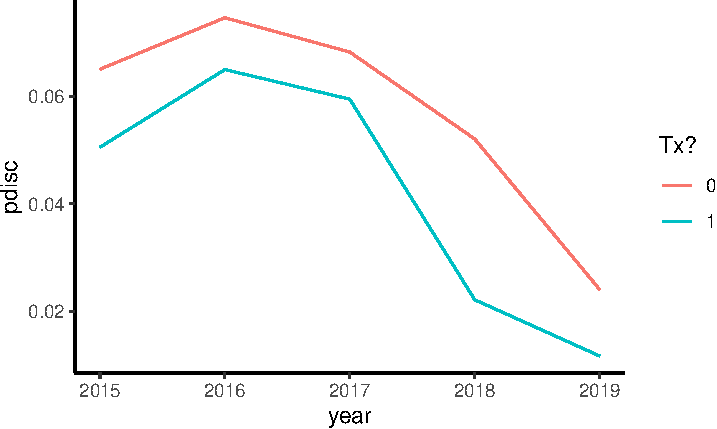
\includegraphics[width=0.75\linewidth]{Designing-Simulations-in-R_files/figure-latex/unnamed-chunk-252-1} \end{center}

Our treatment group drops faster than the control. We see the nonlinear structure actually observed in our original data in terms of discipline over time has been replicated.

We next write some functions to analyze our data.
This should feel very familiar: we are just doing our simulation framework, as usual.

\begin{Shaded}
\begin{Highlighting}[]
\NormalTok{eval\_dat }\OtherTok{=} \ControlFlowTok{function}\NormalTok{( sdat ) \{}
    
    \CommentTok{\# No covariate adjustment, average change model (on log outcome)}
\NormalTok{    M\_raw }\OtherTok{=} \FunctionTok{lm}\NormalTok{( }\FunctionTok{log}\NormalTok{( pdisc\_2018 ) }\SpecialCharTok{\textasciitilde{}} \DecValTok{1} \SpecialCharTok{+}\NormalTok{ Z, }\AttributeTok{data=}\NormalTok{sdat )}

    \CommentTok{\# Simple average change model using 2018 as outcome.}
\NormalTok{    M\_simple }\OtherTok{=} \FunctionTok{lm}\NormalTok{( pdisc\_2018 }\SpecialCharTok{\textasciitilde{}} \DecValTok{1} \SpecialCharTok{+}\NormalTok{ Z }\SpecialCharTok{+}\NormalTok{ pdisc\_2017 }\SpecialCharTok{+}\NormalTok{ pdisc\_2016 }\SpecialCharTok{+}\NormalTok{ pdisc\_2015,}
                   \AttributeTok{data=}\NormalTok{sdat )}

    \CommentTok{\# Simple model on logged outcome}
\NormalTok{    M\_log }\OtherTok{=} \FunctionTok{lm}\NormalTok{( }\FunctionTok{log}\NormalTok{( pdisc\_2018 ) }\SpecialCharTok{\textasciitilde{}} \DecValTok{1} \SpecialCharTok{+}\NormalTok{ Z }\SpecialCharTok{+} \FunctionTok{log}\NormalTok{( pdisc\_2017) }\SpecialCharTok{+} \FunctionTok{log}\NormalTok{( pdisc\_2016) }\SpecialCharTok{+} \FunctionTok{log}\NormalTok{( pdisc\_2015 ),}
                \AttributeTok{data=}\NormalTok{sdat )}
    
    \CommentTok{\# Ratio of average disc to average prior disc as outcome}
\NormalTok{    sdat }\OtherTok{=} \FunctionTok{mutate}\NormalTok{( sdat,}
                   \AttributeTok{avg\_disc =}\NormalTok{ (pdisc\_2018 }\SpecialCharTok{+}\NormalTok{ pdisc\_2019)}\SpecialCharTok{/}\DecValTok{2}\NormalTok{,}
                   \AttributeTok{prior\_disc =}\NormalTok{ (pdisc\_2017 }\SpecialCharTok{+}\NormalTok{ pdisc\_2016 }\SpecialCharTok{+}\NormalTok{ pdisc\_2015 )}\SpecialCharTok{/}\DecValTok{3}\NormalTok{,}
                   \AttributeTok{disc =}\NormalTok{ pdisc\_2018 }\SpecialCharTok{/}\NormalTok{ prior\_disc,}
                   \AttributeTok{disc\_two =}\NormalTok{ avg\_disc }\SpecialCharTok{/}\NormalTok{ prior\_disc )}
\NormalTok{    M\_ratio }\OtherTok{=} \FunctionTok{lm}\NormalTok{( disc }\SpecialCharTok{\textasciitilde{}} \DecValTok{1} \SpecialCharTok{+}\NormalTok{ Z, }\AttributeTok{data =}\NormalTok{ sdat )}
\NormalTok{    M\_ratio\_twopost }\OtherTok{=} \FunctionTok{lm}\NormalTok{( disc\_two }\SpecialCharTok{\textasciitilde{}} \DecValTok{1} \SpecialCharTok{+}\NormalTok{ Z, }\AttributeTok{data =}\NormalTok{ sdat )}
    
    \CommentTok{\# Use average of two post{-}tx time periods, averaged to reduce noise}
\NormalTok{    M\_twopost }\OtherTok{=} \FunctionTok{lm}\NormalTok{( }\FunctionTok{log}\NormalTok{( avg\_disc ) }\SpecialCharTok{\textasciitilde{}} \DecValTok{1} \SpecialCharTok{+}\NormalTok{ Z }\SpecialCharTok{+} \FunctionTok{log}\NormalTok{( pdisc\_2017 ) }\SpecialCharTok{+} \FunctionTok{log}\NormalTok{( pdisc\_2016 ) }\SpecialCharTok{+} \FunctionTok{log}\NormalTok{( pdisc\_2015 ), }\AttributeTok{data=}\NormalTok{sdat )}

    \CommentTok{\# Time and unit fixed effects}
\NormalTok{    sdatL }\OtherTok{=} \FunctionTok{pivot\_longer}\NormalTok{( sdat, }\AttributeTok{cols =}\NormalTok{ pdisc\_2015}\SpecialCharTok{:}\NormalTok{pdisc\_2019, }
                          \AttributeTok{names\_to =} \StringTok{"year"}\NormalTok{,}
                          \AttributeTok{values\_to =} \StringTok{"pdisc"}\NormalTok{ ) }\SpecialCharTok{\%\textgreater{}\%}
        \FunctionTok{mutate}\NormalTok{( }\AttributeTok{Z =}\NormalTok{ Z }\SpecialCharTok{*}\NormalTok{ (year }\SpecialCharTok{\%in\%} \FunctionTok{c}\NormalTok{( }\StringTok{"pdisc\_2018"}\NormalTok{, }\StringTok{"pdisc\_2019"}\NormalTok{ ) ),}
                \AttributeTok{ID =} \FunctionTok{paste0}\NormalTok{( }\StringTok{"S"}\NormalTok{, ID ) )}
    
\NormalTok{    M\_2wfe }\OtherTok{=} \FunctionTok{lm}\NormalTok{( }\FunctionTok{log}\NormalTok{( pdisc ) }\SpecialCharTok{\textasciitilde{}} \DecValTok{0} \SpecialCharTok{+}\NormalTok{ ID }\SpecialCharTok{+}\NormalTok{ year }\SpecialCharTok{+}\NormalTok{ Z,}
                 \AttributeTok{data=}\NormalTok{sdatL )}

    \CommentTok{\# Bundle all our models by getting the estimated treatment impact}
    \CommentTok{\# from each.}
\NormalTok{    models }\OtherTok{\textless{}{-}} \FunctionTok{list}\NormalTok{( }\AttributeTok{raw=}\NormalTok{M\_raw, }\AttributeTok{simple=}\NormalTok{M\_simple,}
                       \AttributeTok{log=}\NormalTok{M\_log, }\AttributeTok{ratio =}\NormalTok{ M\_ratio, }
                       \AttributeTok{ratio\_twopost =}\NormalTok{ M\_ratio\_twopost,}
                       \AttributeTok{log\_twopost =}\NormalTok{ M\_twopost, }
                       \AttributeTok{FE =}\NormalTok{ M\_2wfe )}
\NormalTok{    rs }\OtherTok{\textless{}{-}} \FunctionTok{map\_df}\NormalTok{( models, broom}\SpecialCharTok{::}\NormalTok{tidy, }\AttributeTok{.id=}\StringTok{"model"}\NormalTok{ ) }\SpecialCharTok{\%\textgreater{}\%}
        \FunctionTok{filter}\NormalTok{( term}\SpecialCharTok{==}\StringTok{"Z"}\NormalTok{ ) }\SpecialCharTok{\%\textgreater{}\%}
\NormalTok{        dplyr}\SpecialCharTok{::}\FunctionTok{select}\NormalTok{( }\SpecialCharTok{{-}}\NormalTok{term ) }\SpecialCharTok{\%\textgreater{}\%}
      \FunctionTok{arrange}\NormalTok{( model )}
    
\NormalTok{    rs}
\NormalTok{\}}
\end{Highlighting}
\end{Shaded}

Our method marches through a host of models; we weren't sure what the gains would be from one model to another, so we decided to conduct power analyses on all of them.
Again, we look at what our evaluation function does:

\begin{Shaded}
\begin{Highlighting}[]
\NormalTok{dat }\OtherTok{=} \FunctionTok{make\_dat\_param}\NormalTok{( }\AttributeTok{n\_c =} \DecValTok{4}\NormalTok{, }\AttributeTok{n\_t =} \DecValTok{4}\NormalTok{, }\AttributeTok{tx =} \FloatTok{0.5}\NormalTok{ )}
\FunctionTok{eval\_dat}\NormalTok{( dat )}
\end{Highlighting}
\end{Shaded}

\begin{verbatim}
## # A tibble: 7 x 5
##   model       estimate std.error statistic p.value
##   <chr>          <dbl>     <dbl>     <dbl>   <dbl>
## 1 FE          -0.644      0.325     -1.98   0.0576
## 2 log         -0.841      0.478     -1.76   0.176 
## 3 log_twopost -1.22       0.437     -2.80   0.0680
## 4 ratio       -0.126      0.136     -0.923  0.392 
## 5 ratio_twop~ -0.269      0.139     -1.93   0.102 
## 6 raw         -0.650      0.300     -2.17   0.0733
## 7 simple      -0.00983    0.0133    -0.742  0.512
\end{verbatim}

We have a nice set of estimates, one for each model.

\section{Running the simulation}\label{running-the-simulation-1}

Now we put it all together in our classic simulator:

\begin{Shaded}
\begin{Highlighting}[]
\NormalTok{sim\_run }\OtherTok{=} \ControlFlowTok{function}\NormalTok{( n\_c, n\_t, tx, R, }\AttributeTok{seed =} \ConstantTok{NULL}\NormalTok{ ) \{}
    \ControlFlowTok{if}\NormalTok{ ( }\SpecialCharTok{!}\FunctionTok{is.null}\NormalTok{( seed ) ) \{}
        \FunctionTok{set.seed}\NormalTok{(seed)}
\NormalTok{    \}}
    \FunctionTok{cat}\NormalTok{( }\StringTok{"Running n\_c, n\_t ="}\NormalTok{, n\_c, n\_t, }\StringTok{"tx ="}\NormalTok{, tx, }\StringTok{"}\SpecialCharTok{\textbackslash{}n}\StringTok{"}\NormalTok{ )}
\NormalTok{    rps }\OtherTok{=} \FunctionTok{rerun}\NormalTok{( R, \{}
\NormalTok{        sdat }\OtherTok{=} \FunctionTok{make\_dat\_param}\NormalTok{(}\AttributeTok{n\_c =}\NormalTok{ n\_c, }\AttributeTok{n\_t =}\NormalTok{ n\_t, }\AttributeTok{tx =}\NormalTok{ tx)}
        \FunctionTok{eval\_dat}\NormalTok{( sdat )}
\NormalTok{    \})}
    \FunctionTok{bind\_rows}\NormalTok{( rps )}
\NormalTok{\}}
\end{Highlighting}
\end{Shaded}

We then do the usual to run across a set of scenarios, running \texttt{sim\_run} on each row of the following:

\begin{Shaded}
\begin{Highlighting}[]
\NormalTok{res }\OtherTok{=} \FunctionTok{expand\_grid}\NormalTok{( }\AttributeTok{tx =} \FunctionTok{c}\NormalTok{( }\DecValTok{1}\NormalTok{, }\FloatTok{0.75}\NormalTok{, }\FloatTok{0.5}\NormalTok{ ),}
                   \AttributeTok{n\_c =} \FunctionTok{c}\NormalTok{( }\DecValTok{4}\NormalTok{, }\DecValTok{5}\NormalTok{, }\DecValTok{6}\NormalTok{, }\DecValTok{8}\NormalTok{, }\DecValTok{12}\NormalTok{, }\DecValTok{20}\NormalTok{ ),}
                   \AttributeTok{n\_t =} \FunctionTok{c}\NormalTok{( }\DecValTok{4}\NormalTok{, }\DecValTok{5}\NormalTok{, }\DecValTok{6}\NormalTok{ ) )}
\NormalTok{res}\SpecialCharTok{$}\NormalTok{R }\OtherTok{=} \DecValTok{1000}
\NormalTok{res}\SpecialCharTok{$}\NormalTok{seed }\OtherTok{=} \DecValTok{1010203} \SpecialCharTok{+} \DecValTok{1}\SpecialCharTok{:}\FunctionTok{nrow}\NormalTok{(res)}
\end{Highlighting}
\end{Shaded}

For evaluation, we load our saved results and calculate rejection rates (we use an alpha of 0.10 since we are doing one-sided testing):

\begin{Shaded}
\begin{Highlighting}[]
\NormalTok{res }\OtherTok{=} \FunctionTok{readRDS}\NormalTok{( }\AttributeTok{file=}\StringTok{"data/discipline\_simulation.rds"}\NormalTok{ )}

\NormalTok{sres }\OtherTok{\textless{}{-}}\NormalTok{ res }\SpecialCharTok{\%\textgreater{}\%} \FunctionTok{group\_by}\NormalTok{( n\_c, n\_t, tx, model ) }\SpecialCharTok{\%\textgreater{}\%}
    \FunctionTok{summarise}\NormalTok{( }\AttributeTok{E\_est =} \FunctionTok{mean}\NormalTok{( estimate ),}
               \AttributeTok{SE =} \FunctionTok{sd}\NormalTok{( estimate ),}
               \AttributeTok{E\_SE\_hat =} \FunctionTok{mean}\NormalTok{( std.error ),}
               \AttributeTok{pow =} \FunctionTok{mean}\NormalTok{( p.value }\SpecialCharTok{\textless{}=} \FloatTok{0.10}\NormalTok{ ) ) }\CommentTok{\# one{-}sided testing}
\NormalTok{sres}
\end{Highlighting}
\end{Shaded}

\begin{verbatim}
## # A tibble: 378 x 8
## # Groups:   n_c, n_t, tx [54]
##      n_c   n_t    tx model   E_est     SE E_SE_hat
##    <dbl> <dbl> <dbl> <chr>   <dbl>  <dbl>    <dbl>
##  1     4     4  0.5  FE    -0.693  0.313    0.277 
##  2     4     4  0.5  log   -0.694  0.476    0.430 
##  3     4     4  0.5  log_~ -0.692  0.431    0.383 
##  4     4     4  0.5  ratio -0.374  0.219    0.203 
##  5     4     4  0.5  rati~ -0.291  0.151    0.139 
##  6     4     4  0.5  raw   -0.719  0.535    0.515 
##  7     4     4  0.5  simp~ -0.0195 0.0194   0.0157
##  8     4     4  0.75 FE    -0.292  0.310    0.274 
##  9     4     4  0.75 log   -0.295  0.488    0.435 
## 10     4     4  0.75 log_~ -0.305  0.424    0.373 
## # i 368 more rows
## # i 1 more variable: pow <dbl>
\end{verbatim}

\section{Evaluating power}\label{evaluating-power}

Once our simulation is run, we can explore power as a function of the design characteristics.
In particular, we eventually want to calculate the chance of noticing effects of different sizes, given various sample sizes we might employ.
Our driving question is how few schools on the treated side can we get away with?
Also, we want to know how much having more schools on the control side allows us to get away with fewer schools on the treated side.

\subsection{Checking validity of our models}\label{checking-validity-of-our-models}

Before we look at power, we need to check on whether our different models are valid.
This is especiallt important as we are in a small \(n\) context, so we know asymptotics may not hold as they should.
To check our models for validity we subset our trials to where \texttt{tx\ =\ 1}, and look at the rejection rates.

We first run a regression to see if rejection is a function of sample size (are smaller samples more invalid) and treatment-control imbalance.
We center both variables so our intercepts are overall average rejection rates for each model considered:

\begin{Shaded}
\begin{Highlighting}[]
\NormalTok{sres }\OtherTok{=} \FunctionTok{mutate}\NormalTok{( sres,}
               \AttributeTok{n =}\NormalTok{ n\_c }\SpecialCharTok{+}\NormalTok{ n\_t,}
               \AttributeTok{imbalance =} \FunctionTok{pmax}\NormalTok{( n\_t }\SpecialCharTok{/}\NormalTok{ n\_c, n\_c }\SpecialCharTok{/}\NormalTok{ n\_t ) }\SpecialCharTok{{-}} \DecValTok{1}\NormalTok{ )}
\NormalTok{sres}\SpecialCharTok{$}\NormalTok{n }\OtherTok{=}\NormalTok{ (sres}\SpecialCharTok{$}\NormalTok{n }\SpecialCharTok{{-}} \FunctionTok{mean}\NormalTok{(sres}\SpecialCharTok{$}\NormalTok{n)) }\SpecialCharTok{/} \FunctionTok{sd}\NormalTok{(sres}\SpecialCharTok{$}\NormalTok{n)}
\NormalTok{mod }\OtherTok{=} \FunctionTok{lm}\NormalTok{( pow }\SpecialCharTok{\textasciitilde{}} \DecValTok{0} \SpecialCharTok{+}\NormalTok{ (n }\SpecialCharTok{+}\NormalTok{ imbalance) }\SpecialCharTok{*}\NormalTok{ model }\SpecialCharTok{{-}}\NormalTok{ n }\SpecialCharTok{{-}}\NormalTok{ imbalance,}
          \AttributeTok{data =} \FunctionTok{filter}\NormalTok{( sres, tx }\SpecialCharTok{==} \DecValTok{1}\NormalTok{ ) )}
\NormalTok{broom}\SpecialCharTok{::}\FunctionTok{tidy}\NormalTok{(mod) }\SpecialCharTok{\%\textgreater{}\%}
\NormalTok{  knitr}\SpecialCharTok{::}\FunctionTok{kable}\NormalTok{( }\AttributeTok{digits =} \DecValTok{3}\NormalTok{)}
\end{Highlighting}
\end{Shaded}

\begin{tabular}{l|r|r|r|r}
\hline
term & estimate & std.error & statistic & p.value\\
\hline
modelFE & 0.143 & 0.006 & 24.593 & 0.000\\
\hline
modellog & 0.099 & 0.006 & 16.999 & 0.000\\
\hline
modellog\_twopost & 0.093 & 0.006 & 15.939 & 0.000\\
\hline
modelratio & 0.090 & 0.006 & 15.437 & 0.000\\
\hline
modelratio\_twopost & 0.093 & 0.006 & 15.967 & 0.000\\
\hline
modelraw & 0.092 & 0.006 & 15.751 & 0.000\\
\hline
modelsimple & 0.091 & 0.006 & 15.571 & 0.000\\
\hline
n:modelFE & -0.003 & 0.006 & -0.459 & 0.647\\
\hline
n:modellog & 0.001 & 0.006 & 0.141 & 0.888\\
\hline
n:modellog\_twopost & -0.005 & 0.006 & -0.919 & 0.360\\
\hline
n:modelratio & 0.000 & 0.006 & 0.071 & 0.944\\
\hline
n:modelratio\_twopost & 0.002 & 0.006 & 0.414 & 0.680\\
\hline
n:modelraw & -0.006 & 0.006 & -1.008 & 0.316\\
\hline
n:modelsimple & 0.001 & 0.006 & 0.191 & 0.849\\
\hline
imbalance:modelFE & 0.005 & 0.005 & 0.857 & 0.394\\
\hline
imbalance:modellog & -0.003 & 0.005 & -0.587 & 0.558\\
\hline
imbalance:modellog\_twopost & 0.004 & 0.005 & 0.708 & 0.480\\
\hline
imbalance:modelratio & 0.000 & 0.005 & -0.001 & 0.999\\
\hline
imbalance:modelratio\_twopost & 0.001 & 0.005 & 0.249 & 0.804\\
\hline
imbalance:modelraw & 0.006 & 0.005 & 1.154 & 0.251\\
\hline
imbalance:modelsimple & 0.001 & 0.005 & 0.180 & 0.858\\
\hline
\end{tabular}

We can also plot the nominal rejection rates under the null:

\begin{Shaded}
\begin{Highlighting}[]
\NormalTok{sres }\SpecialCharTok{\%\textgreater{}\%} \FunctionTok{filter}\NormalTok{( tx }\SpecialCharTok{==} \DecValTok{1}\NormalTok{ ) }\SpecialCharTok{\%\textgreater{}\%}
\FunctionTok{ggplot}\NormalTok{( }\FunctionTok{aes}\NormalTok{( n\_c, pow, }\AttributeTok{col=}\NormalTok{model ) ) }\SpecialCharTok{+}
  \FunctionTok{facet\_wrap}\NormalTok{( }\SpecialCharTok{\textasciitilde{}}\NormalTok{ n\_t, }\AttributeTok{nrow=}\DecValTok{1}\NormalTok{ ) }\SpecialCharTok{+}
  \FunctionTok{geom\_line}\NormalTok{() }\SpecialCharTok{+}
  \FunctionTok{geom\_hline}\NormalTok{( }\AttributeTok{yintercept =} \FloatTok{0.10}\NormalTok{ ) }\SpecialCharTok{+}
  \FunctionTok{scale\_x\_log10}\NormalTok{(}\AttributeTok{breaks=}\FunctionTok{unique}\NormalTok{(sres}\SpecialCharTok{$}\NormalTok{n\_c) )}
\end{Highlighting}
\end{Shaded}

\begin{center}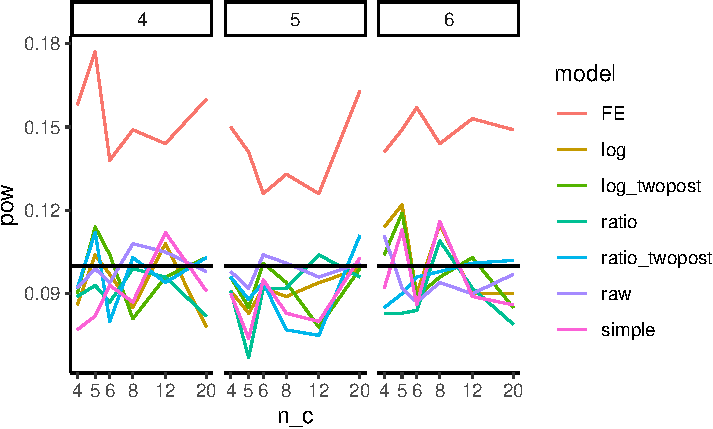
\includegraphics[width=0.75\linewidth]{Designing-Simulations-in-R_files/figure-latex/unnamed-chunk-258-1} \end{center}

We see the fixed effect models have elevated rates of rejection.
Interestingly, these rates do not seem particularly dependent on sample size or treatment-control imbalance (note lack of significant coefficeints on our regression model).
The other models all appear valid.

We can also check for bias of our methods:

\begin{Shaded}
\begin{Highlighting}[]
\NormalTok{sres }\SpecialCharTok{\%\textgreater{}\%} \FunctionTok{group\_by}\NormalTok{( model, tx ) }\SpecialCharTok{\%\textgreater{}\%}
  \FunctionTok{summarise}\NormalTok{( }\AttributeTok{E\_est =} \FunctionTok{mean}\NormalTok{( E\_est ) ) }\SpecialCharTok{\%\textgreater{}\%}
  \FunctionTok{pivot\_wider}\NormalTok{( }\AttributeTok{names\_from=}\StringTok{"tx"}\NormalTok{, }\AttributeTok{values\_from=}\StringTok{"E\_est"}\NormalTok{ )}
\end{Highlighting}
\end{Shaded}

\begin{verbatim}
## # A tibble: 7 x 4
## # Groups:   model [7]
##   model           `0.5`  `0.75`        `1`
##   <chr>           <dbl>   <dbl>      <dbl>
## 1 FE            -0.692  -0.290  -0.000703 
## 2 log           -0.692  -0.288   0.00120  
## 3 log_twopost   -0.692  -0.291   0.00241  
## 4 ratio         -0.372  -0.187  -0.000937 
## 5 ratio_twopost -0.289  -0.145  -0.00108  
## 6 raw           -0.694  -0.290   0.00327  
## 7 simple        -0.0206 -0.0104  0.0000998
\end{verbatim}

We see our models are estimating different things, none of which are the treatment effect as we parameterized it.
In particular, ``FE,'' ``log,'' ``raw,'' and ``log\_twopost'' are all estimating the impact on the log scale.
Note that \(log( 0.5 ) \approx -0.69\) and \(log( 0.75 ) \approx -0.29\).
Our ``simple'' estimator is estimating the impact on the absolute scale; reducing discipline rates by 50\% corresponds to about a 2\% reduction in actual cases.
Finally, ``ratio'' and ``ratio\_twopost'' are estimating the change in the average ratio of post-policy discipline to pre; they are akin to a gain score as compared to the log regressions.

\subsection{Assessing Precision (SE)}\label{assessing-precision-se}

Now, which methods are the most precise?
We look at the true standard errors across our methods (we drop ``simple'' and the ``ratio'' estimators since they are not on the ratio scale):

\begin{Shaded}
\begin{Highlighting}[]
\NormalTok{sres }\SpecialCharTok{\%\textgreater{}\%} 
  \FunctionTok{group\_by}\NormalTok{( model, n\_c, n\_t ) }\SpecialCharTok{\%\textgreater{}\%}
  \FunctionTok{summarise}\NormalTok{( }\AttributeTok{SE =} \FunctionTok{mean}\NormalTok{(SE ) ) }\SpecialCharTok{\%\textgreater{}\%}
  \FunctionTok{filter}\NormalTok{( }\SpecialCharTok{!}\NormalTok{(model }\SpecialCharTok{\%in\%} \FunctionTok{c}\NormalTok{( }\StringTok{"simple"}\NormalTok{, }\StringTok{"ratio"}\NormalTok{, }\StringTok{"ratio\_twopost"}\NormalTok{ ) ) ) }\SpecialCharTok{\%\textgreater{}\%}
  \FunctionTok{ggplot}\NormalTok{( }\FunctionTok{aes}\NormalTok{( n\_c, SE, }\AttributeTok{col=}\NormalTok{model )) }\SpecialCharTok{+}
    \FunctionTok{facet\_grid}\NormalTok{( . }\SpecialCharTok{\textasciitilde{}}\NormalTok{ n\_t ) }\SpecialCharTok{+}
    \FunctionTok{geom\_line}\NormalTok{() }\SpecialCharTok{+} \FunctionTok{geom\_point}\NormalTok{() }\SpecialCharTok{+}
    \FunctionTok{geom\_hline}\NormalTok{( }\AttributeTok{yintercept =} \DecValTok{0}\NormalTok{ ) }\SpecialCharTok{+}
  \FunctionTok{labs}\NormalTok{( }\AttributeTok{colour =} \StringTok{"Model"}\NormalTok{ )}
\end{Highlighting}
\end{Shaded}

\begin{center}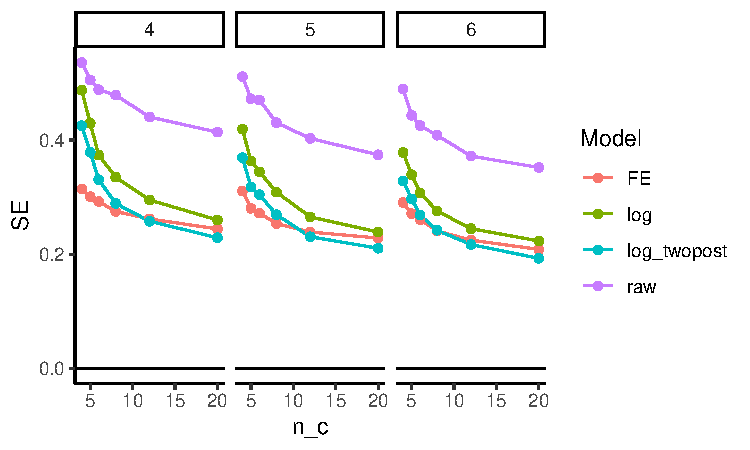
\includegraphics[width=0.75\linewidth]{Designing-Simulations-in-R_files/figure-latex/disc_precision-1} \end{center}

It looks like averaging two years for the outcome is helpful, and bumps up precision.
The two way fixed effects model seems to react to the number of control units differently than the other estimators; it is way more precise when the number of controls is few, but the other estimators catch up.
The ``raw'' estimator gives a baseline of no covariate adjustment; everything is substantially more precise than it.
The covariates matter a lot.

\subsection{Assessing power}\label{assessing-power}

We next look at power over our explored contexts, for the models that we find to be valid (i.e., not FE).

\begin{Shaded}
\begin{Highlighting}[]
\NormalTok{sres }\SpecialCharTok{\%\textgreater{}\%} 
  \FunctionTok{filter}\NormalTok{( model }\SpecialCharTok{!=} \StringTok{"FE"}\NormalTok{,tx }\SpecialCharTok{!=} \DecValTok{1}\NormalTok{ ) }\SpecialCharTok{\%\textgreater{}\%}
  \FunctionTok{ggplot}\NormalTok{( }\FunctionTok{aes}\NormalTok{( n\_c, pow, }\AttributeTok{col=}\NormalTok{model )) }\SpecialCharTok{+}
    \FunctionTok{facet\_grid}\NormalTok{(  . }\SpecialCharTok{\textasciitilde{}}\NormalTok{ tx }\SpecialCharTok{+}\NormalTok{ n\_t, }\AttributeTok{labeller =}\NormalTok{ label\_both ) }\SpecialCharTok{+}
    \FunctionTok{geom\_line}\NormalTok{() }\SpecialCharTok{+} \FunctionTok{geom\_point}\NormalTok{() }\SpecialCharTok{+}
    \FunctionTok{geom\_hline}\NormalTok{( }\AttributeTok{yintercept =} \DecValTok{0}\NormalTok{, }\AttributeTok{col=}\StringTok{"grey"}\NormalTok{ ) }\SpecialCharTok{+}
    \FunctionTok{geom\_hline}\NormalTok{( }\AttributeTok{yintercept =} \FunctionTok{c}\NormalTok{( }\FloatTok{0.10}\NormalTok{, }\FloatTok{0.80}\NormalTok{ ), }\AttributeTok{lty=}\DecValTok{2}\NormalTok{ ) }\SpecialCharTok{+}
  \FunctionTok{theme\_minimal}\NormalTok{()}\SpecialCharTok{+} \FunctionTok{theme}\NormalTok{( }\AttributeTok{legend.position=}\StringTok{"bottom"}\NormalTok{,}
                          \AttributeTok{legend.direction=}\StringTok{"horizontal"}\NormalTok{,}
                          \AttributeTok{legend.key.width=}\FunctionTok{unit}\NormalTok{(}\DecValTok{1}\NormalTok{,}\StringTok{"cm"}\NormalTok{),}
                          \AttributeTok{panel.border =} \FunctionTok{element\_blank}\NormalTok{() ) }\SpecialCharTok{+}
  \FunctionTok{labs}\NormalTok{( }\AttributeTok{title=}\StringTok{"Power for various methods vs number of controls."}\NormalTok{,}
      \AttributeTok{y =} \StringTok{"Power"}\NormalTok{ )}
\end{Highlighting}
\end{Shaded}

\begin{center}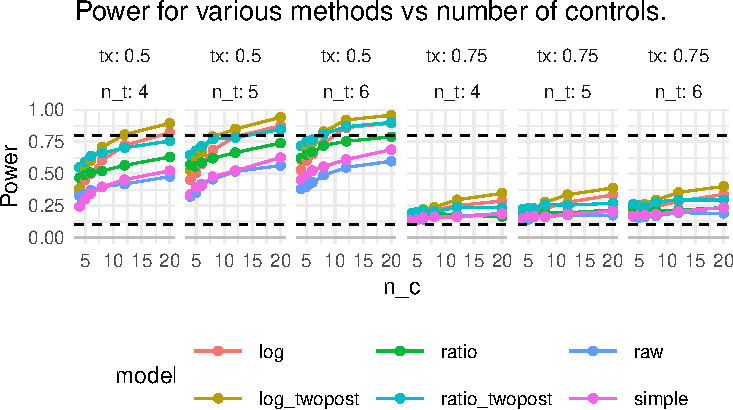
\includegraphics[width=0.75\linewidth]{Designing-Simulations-in-R_files/figure-latex/disc_power-1} \end{center}

We mark 80\% power with a dashed line. For a 25\% reduction in discipline, nothing reaches desired levels of power.
For 50\% reduction, some designs do, but we need substantial numbers of control schools.
Averaging two years of outcomes post-treatment seems important: the ``twopost'' methods have a distinct power bump.
For a single year of outcome data, the log model seems our best bet.

\subsection{Assessing Minimum Detectable Effects}\label{assessing-minimum-detectable-effects}

Sometimes we want to know, given a design, what size effect we might be able to detect.
The usual measure for this is the Minimum Detectable Effect (MDE), which is usually the size of the smallest effect we could detect with power 80\%.

To calculate Minimal Detectable Effects (MDEs) for the log-scale estimators,
we first average our SEs over our different designs, grouped by sample size, and then convert the SEs to MDEs by multiplying by 2.8.
We then have to convert to our treatment scale by flipping the sign and exponentiating, to get out of the log scale.

\begin{Shaded}
\begin{Highlighting}[]
\NormalTok{sres2 }\OtherTok{=}\NormalTok{ sres }\SpecialCharTok{\%\textgreater{}\%} 
  \FunctionTok{group\_by}\NormalTok{( model, n\_c, n\_t ) }\SpecialCharTok{\%\textgreater{}\%}
  \FunctionTok{summarise}\NormalTok{( }\AttributeTok{SE =} \FunctionTok{mean}\NormalTok{( SE ),}
             \AttributeTok{E\_SE\_hat =} \FunctionTok{mean}\NormalTok{( E\_SE\_hat ) ) }\SpecialCharTok{\%\textgreater{}\%}
  \FunctionTok{mutate}\NormalTok{( }\AttributeTok{MDE =} \FunctionTok{exp}\NormalTok{( }\SpecialCharTok{{-}}\NormalTok{ (}\FloatTok{1.64} \SpecialCharTok{+} \FloatTok{0.8}\NormalTok{) }\SpecialCharTok{*}\NormalTok{ SE ) )}

\NormalTok{sres2 }\SpecialCharTok{\%\textgreater{}\%} 
  \FunctionTok{filter}\NormalTok{( }\SpecialCharTok{!}\NormalTok{(model }\SpecialCharTok{\%in\%} \FunctionTok{c}\NormalTok{( }\StringTok{"simple"}\NormalTok{, }\StringTok{"ratio"}\NormalTok{, }\StringTok{"ratio\_twopost"}\NormalTok{ ) ) ) }\SpecialCharTok{\%\textgreater{}\%}
  \FunctionTok{ggplot}\NormalTok{( }\FunctionTok{aes}\NormalTok{( n\_c, MDE, }\AttributeTok{col=}\NormalTok{model ) ) }\SpecialCharTok{+}
  \FunctionTok{facet\_wrap}\NormalTok{( }\SpecialCharTok{\textasciitilde{}}\NormalTok{ n\_t, }\AttributeTok{labeller =}\NormalTok{ label\_both ) }\SpecialCharTok{+}
  \FunctionTok{geom\_point}\NormalTok{() }\SpecialCharTok{+} \FunctionTok{geom\_line}\NormalTok{()  }\SpecialCharTok{+}
  \FunctionTok{geom\_hline}\NormalTok{( }\AttributeTok{yintercept =} \FloatTok{0.5}\NormalTok{ ) }\SpecialCharTok{+}
  \FunctionTok{theme\_minimal}\NormalTok{() }\SpecialCharTok{+}
  \FunctionTok{scale\_x\_log10}\NormalTok{( }\AttributeTok{breaks =} \FunctionTok{unique}\NormalTok{( sres}\SpecialCharTok{$}\NormalTok{n\_c ) ) }\SpecialCharTok{+}
  \FunctionTok{theme}\NormalTok{( }\AttributeTok{legend.position=}\StringTok{"bottom"}\NormalTok{,}
         \AttributeTok{legend.direction=}\StringTok{"horizontal"}\NormalTok{, }\AttributeTok{legend.key.width=}\FunctionTok{unit}\NormalTok{(}\DecValTok{1}\NormalTok{,}\StringTok{"cm"}\NormalTok{),}
         \AttributeTok{panel.border =} \FunctionTok{element\_blank}\NormalTok{() ) }\SpecialCharTok{+}
  \FunctionTok{labs}\NormalTok{( }\AttributeTok{x =} \StringTok{"Number of control units"}\NormalTok{, }\AttributeTok{y =} \StringTok{"MDE (proportion reduction of rate)"}\NormalTok{,}
        \AttributeTok{caption =} \StringTok{"A MDE of 0.6 means a 60\% reduction (more than half) in discipline rates"}\NormalTok{,}
        \AttributeTok{title =} \StringTok{"MDE vs number of control units for various methods"}\NormalTok{ )}
\end{Highlighting}
\end{Shaded}

\begin{center}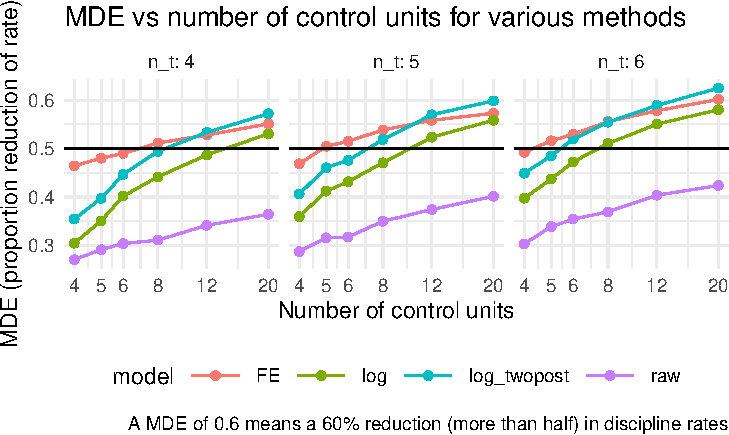
\includegraphics[width=0.75\linewidth]{Designing-Simulations-in-R_files/figure-latex/disc_mde-1} \end{center}

Corresponding with our findings regarding precision, above, the twopost estimator is the most sensitive, finding the smallest effects.

\chapter{Simulation under the Potential Outcomes Framework}\label{chap-potential-outcomes}

If we are in the business of evaluating how various methods such as matching or propensity score weighting work in practice, we would probably turn to the potential outcomes framework for our simulations.
The potential outcomes framework is a framework typically used in the causal inference literature to make very explicit statements regarding the mechanics of causality and the associated estimands one might target when estimating causal effects.
While we recommend reading, for a more thourough overview, either {[}CITE Raudenbush or Field Experiments textbook{]}, we briefly outline this framework here to set out our notation.

Take a sample of experimental units, indexed by \(i\).
For each unit, we can treat it or not.
Denote treatment as \(Z_i = 1\) for treated or \(Z_i = 0\) for not treated.
Now we imagine each unit has two potential outcomes being the outcome we would see if we treated it (\(Y_i(1)\)) or if we did not (\(Y_i(0)\)).
Finally, our observed outcome is then
\[ Y_i^{obs} = Z_i Y_i(1) + (1-Z_i)Y_i(0) .\]
For a unit, the treatment effect is \(\tau_i = Y_i(1) - Y_i(0)\); it is how much our outcome changes if we treat vs.~not treat.
Frustratingly, for each unit we can only see one of its two potential outcomes, so we can never get an estimate of these individual \(\tau_i\).
Under this view, causality is a missing data problem: if we only were able to impute the missing potential outcomes, we could have a dataset where we could calculate any estimands we wanted. E.g., the true average treatment effect \emph{for the sample} \(\mathcal{S}\) would be:

\[ ATE_{\mathcal{S}} = \frac{1}{N} \sum_{i} Y_i(1) - Y_i( 0 ) . \]
The average proportion increase, by contrast, would be

\[ API_{\mathcal{S}} = \frac{1}{N} \sum_{i} \frac{Y_i(1)}{Y_i(0)} \]

\section{Finite vs.~Superpopulation inference}\label{finite-vs.-superpopulation-inference}

Consider a sample of \(n\) units, \(\mathcal{S}\), along with their set of potential outcomes.
We can talk about the true ATE of the sample, or, if we thought of the sample as being drawn from some larger population, we could talk about the true ATE of that larger population.

This is a tension that often arises in potential outcomes based simulations: if we are focused on \(ATE_{\mathcal{S}}\) then for each sample we generate, our estimand could be (maybe only slightly) different, depending on whether our sample has more or fewer units with high \(\tau_i\).
If, on the other hand, we are focused on where the units came from (which is our data generating model), our estimand is a property of the DGP, and would be the same for each sample generated.

The catch is when we calculate our performance metrics, we now have two possible targets to pick from.
Furthermore, if we are targeting the superpopulation ATE, then our error in estimation may be due in part to the representativeness of the sample, \emph{not} the estimation or uncertainty due to the random assignment.

We will follow this theme throughout this chapter.

\section{Data generation processes for potential outcomes}\label{data-generation-processes-for-potential-outcomes}

If we want to write a simulation using the potential outcomes framework, it is clear and transparent to first generate a complete set of potential outcomes, then generate a random assignment based on some assignment mechanism, and finally generate the observed outcomes as a function of assignment and original potential outcomes.

For example, we might say that our data generation process is as follows: First generate each unit \(i = 1, \ldots, n\), as
\[
\begin{aligned}
X_i &\sim exp( 1 ) - 1 \\
Y_i(0) &= \beta_0 + \beta_1 X_i + \epsilon_i \mbox{ with } \epsilon_i \sim N( 0, \sigma^2 ) \\
\tau_i &= \tau_0 + \tau_1 X_i + \alpha u_i \mbox{ with } u_i \sim t_{df} \\
Y_i(1) &= Y_i(0) + \tau_i 
\end{aligned}
\]
with \(exp(1)\) being the standard exponential distribution and \(t_{df}\) being a \(t\) distribution with \(df\) degrees of freedom.
We subtract 1 from \(X_i\) to zero-center it (it is often convenient to have zero-centered covariates so we can then, e.g., interpret \(\tau_0\) as the true superpopulation ATE of our experiment).

The above model is saying that we first, for each unit, generate a covariate.
We then generate our two potential outcomes.
I.e., we are generating what the outcome would be for each unit if it were treated and if it were not treated.
We are driving both the level and the treatment effect with \(X_i\), assuming \(\beta_1\) and \(\tau_1\) are non-zero.

One advantage of generating all the potential outcomes is we can then calculate the finite-sample estimands such as the true average treatment effect for the generated sample: we just take the average of \(Y_i(1) - Y_i(0)\) for our sample.

Here is some code to illustrate the first part of the data generating process (we leave treatment assignment to later):

\begin{Shaded}
\begin{Highlighting}[]
\NormalTok{gen\_data }\OtherTok{\textless{}{-}} \ControlFlowTok{function}\NormalTok{( }\AttributeTok{n =} \DecValTok{100}\NormalTok{,}
                      \AttributeTok{R2 =} \FloatTok{0.5}\NormalTok{,}
                      \AttributeTok{beta\_0 =} \DecValTok{0}\NormalTok{, }\AttributeTok{beta\_1 =} \DecValTok{1}\NormalTok{,}
                      \AttributeTok{tau\_0 =} \DecValTok{1}\NormalTok{, }\AttributeTok{tau\_1 =} \DecValTok{1}\NormalTok{, }
                      \AttributeTok{alpha =} \DecValTok{1}\NormalTok{, }\AttributeTok{df =} \DecValTok{3}\NormalTok{ ) \{}
  \FunctionTok{stopifnot}\NormalTok{( R2 }\SpecialCharTok{\textgreater{}=} \DecValTok{0} \SpecialCharTok{\&\&}\NormalTok{ R2 }\SpecialCharTok{\textless{}} \DecValTok{1}\NormalTok{ )}
\NormalTok{  X\_i }\OtherTok{=} \FunctionTok{rexp}\NormalTok{( n, }\AttributeTok{rate =} \DecValTok{1}\NormalTok{ ) }\SpecialCharTok{{-}} \DecValTok{1}
\NormalTok{  beta\_1 }\OtherTok{=} \FunctionTok{sqrt}\NormalTok{( }\DecValTok{1} \SpecialCharTok{{-}}\NormalTok{ R2 )}
\NormalTok{  sigma\_e }\OtherTok{=} \FunctionTok{sqrt}\NormalTok{( R2 )}
\NormalTok{  Y0\_i }\OtherTok{=}\NormalTok{ beta\_0 }\SpecialCharTok{+}\NormalTok{ beta\_1 }\SpecialCharTok{*}\NormalTok{ X\_i }\SpecialCharTok{+} \FunctionTok{rnorm}\NormalTok{( n, }\AttributeTok{sd=}\NormalTok{sigma\_e )}
\NormalTok{  tau\_i }\OtherTok{=}\NormalTok{ tau\_0 }\SpecialCharTok{+}\NormalTok{ tau\_1 }\SpecialCharTok{*}\NormalTok{ X\_i }\SpecialCharTok{+}\NormalTok{ alpha }\SpecialCharTok{*} \FunctionTok{rt}\NormalTok{( n, }\AttributeTok{df =}\NormalTok{ df )}
\NormalTok{  Y1\_i }\OtherTok{=}\NormalTok{ Y0\_i }\SpecialCharTok{+}\NormalTok{ tau\_i}
  
  \FunctionTok{tibble}\NormalTok{( }\AttributeTok{X =}\NormalTok{ X\_i, }\AttributeTok{Y0 =}\NormalTok{ Y0\_i, }\AttributeTok{Y1 =}\NormalTok{ Y1\_i )}
\NormalTok{\}}
\end{Highlighting}
\end{Shaded}

And now we see our estimand can change:

\begin{Shaded}
\begin{Highlighting}[]
\FunctionTok{set.seed}\NormalTok{( }\DecValTok{40454}\NormalTok{ )}
\NormalTok{d1 }\OtherTok{\textless{}{-}} \FunctionTok{gen\_data}\NormalTok{( }\DecValTok{50}\NormalTok{ )}
\FunctionTok{mean}\NormalTok{( d1}\SpecialCharTok{$}\NormalTok{Y1 }\SpecialCharTok{{-}}\NormalTok{ d1}\SpecialCharTok{$}\NormalTok{Y0 )}
\end{Highlighting}
\end{Shaded}

\begin{verbatim}
## [1] 0.6374925
\end{verbatim}

\begin{Shaded}
\begin{Highlighting}[]
\NormalTok{d2 }\OtherTok{\textless{}{-}} \FunctionTok{gen\_data}\NormalTok{( }\DecValTok{50}\NormalTok{ )}
\FunctionTok{mean}\NormalTok{( d2}\SpecialCharTok{$}\NormalTok{Y1 }\SpecialCharTok{{-}}\NormalTok{ d2}\SpecialCharTok{$}\NormalTok{Y0 )}
\end{Highlighting}
\end{Shaded}

\begin{verbatim}
## [1] 0.5479788
\end{verbatim}

In reviewing our code, we know our superpopulation ATE should be \texttt{tau}, or 1 exactly.
If our estimate for \texttt{d1} is 0.6 do we say that is close or far from the target?
From a finite sample performance approach, we nailed it.
From superpopulation, less so.

Also in looking at the above, there are a few details to call out:

\begin{itemize}
\tightlist
\item
  We can store the latent, intermediate quantities (both potential outcomes, in particular) so we can calculate the estimands of interest or learn about our data generating process. When we hand the data to an estimator, we would not provide this ``secret'' information.
\item
  We are using a trick to index our DGP by an R2 value rather than coefficients on X so we can have a standardized control-side outcome (the expected variation of \(Y_i(0)\) will be 1). The treatment outcomes will have more variation due to the heterogeniety of the treatment impacts.
\item
  If we were generating data with a constant treatment impact, then \(ATE_{\mathcal{S}} = ATE\) always; this is typical for many similations in the literature. That being said, treatment variation is what causes a lot of methods to fail and so having simulations that have this variation is usually important.
\end{itemize}

Once we have our \emph{schedule of potential outcomes}, we would then generate the \emph{observed outcomes} by assigning our (synthetic, randomly generated) \(n\) units to treatment or control.
For example, say we wanted to simulate an observational context where treatment was a function of our covariate.
We could model each unit as flipping a weighted coin with some probability that was a function of \(X_i\) as so:

\[
\begin{aligned}
p_i &= logit^{-1}( \xi_0 + \xi_1 X_i ) \\
Z_i &= Bern( p_i ) \\
Y_i &= Z_i Y_i(1) + (1-Z_i) Y_i(0) 
\end{aligned}
\]

Here is code for assigning our data to treatment and control:

\begin{Shaded}
\begin{Highlighting}[]
\NormalTok{assign\_data }\OtherTok{\textless{}{-}} \ControlFlowTok{function}\NormalTok{( dat,}
                         \AttributeTok{xi\_0 =} \SpecialCharTok{{-}}\DecValTok{1}\NormalTok{, }\AttributeTok{xi\_1 =} \DecValTok{1}\NormalTok{ ) \{}
\NormalTok{  n }\OtherTok{=} \FunctionTok{nrow}\NormalTok{(dat)}
\NormalTok{  dat }\OtherTok{=} \FunctionTok{mutate}\NormalTok{( dat,}
                \AttributeTok{p =}\NormalTok{ arm}\SpecialCharTok{::}\FunctionTok{invlogit}\NormalTok{( xi\_0 }\SpecialCharTok{+}\NormalTok{ xi\_1 }\SpecialCharTok{*}\NormalTok{ X ),}
                \AttributeTok{Z =} \FunctionTok{rbinom}\NormalTok{( n, }\DecValTok{1}\NormalTok{, }\AttributeTok{prob=}\NormalTok{p ),}
                \AttributeTok{Yobs =} \FunctionTok{ifelse}\NormalTok{( Z }\SpecialCharTok{==} \DecValTok{1}\NormalTok{, Y1, Y0 ) )}
\NormalTok{  dat}
\NormalTok{\}}
\end{Highlighting}
\end{Shaded}

We can then add our assignment variable to our given data as so:

\begin{Shaded}
\begin{Highlighting}[]
\FunctionTok{assign\_data}\NormalTok{( d2 )}
\end{Highlighting}
\end{Shaded}

\begin{verbatim}
## # A tibble: 50 x 6
##           X     Y0      Y1     p     Z    Yobs
##       <dbl>  <dbl>   <dbl> <dbl> <int>   <dbl>
##  1  0.670    0.667   2.58  0.418     1   2.58 
##  2  0.371    0.314   4.57  0.348     1   4.57 
##  3  1.94     1.29    3.03  0.719     0   1.29 
##  4 -0.244    0.119 -10.0   0.224     1 -10.0  
##  5  0.00850  1.44    2.88  0.271     0   1.44 
##  6  1.41     1.14    5.02  0.600     1   5.02 
##  7 -0.864    0.461   0.802 0.134     1   0.802
##  8 -0.00533 -0.914  -1.17  0.268     0  -0.914
##  9 -0.907   -0.202   0.555 0.129     1   0.555
## 10 -0.363   -0.141   1.16  0.204     1   1.16 
## # i 40 more rows
\end{verbatim}

Note how \texttt{Yobs} is, depending on \texttt{Z}, either \texttt{Y0} or \texttt{Y1}.
Separating our our DGP and our random assignment underscores the potential outcomes framework adage of the data are what they are, and we the experimenters (or nature) is randomly assigning these whole units to various conditions and observing the consequences.

In general, we might instead put the \texttt{p\_i} part of the model in our code generating the outcomes, if we wanted to view the chance of treatment assignment as inherent to the unit (which is what we usually expect in an observational context).

\section{Finite sample performance measures}\label{finite-sample-performance-measures}

Let's generate a single dataset with our DGP from above, and run a small experiment where we actually randomize units to treatment and control:

\begin{Shaded}
\begin{Highlighting}[]
\NormalTok{n }\OtherTok{=} \DecValTok{100}
\FunctionTok{set.seed}\NormalTok{(}\DecValTok{442423}\NormalTok{)}
\NormalTok{dat }\OtherTok{=} \FunctionTok{gen\_data}\NormalTok{(n, }\AttributeTok{tau\_1 =} \SpecialCharTok{{-}}\DecValTok{1}\NormalTok{)}
\NormalTok{dat }\OtherTok{=} \FunctionTok{mutate}\NormalTok{( dat,}
              \AttributeTok{Z =} \DecValTok{0} \SpecialCharTok{+}\NormalTok{ (}\FunctionTok{sample}\NormalTok{( n ) }\SpecialCharTok{\textless{}=}\NormalTok{ n}\SpecialCharTok{/}\DecValTok{2}\NormalTok{),}
              \AttributeTok{Yobs =} \FunctionTok{ifelse}\NormalTok{( Z }\SpecialCharTok{==} \DecValTok{1}\NormalTok{, Y1, Y0 ) )}
\NormalTok{mod }\OtherTok{=} \FunctionTok{lm}\NormalTok{( Yobs }\SpecialCharTok{\textasciitilde{}}\NormalTok{ Z, }\AttributeTok{data=}\NormalTok{dat )}
\FunctionTok{coef}\NormalTok{(mod)[[}\StringTok{"Z"}\NormalTok{]]}
\end{Highlighting}
\end{Shaded}

\begin{verbatim}
## [1] 0.8914992
\end{verbatim}

We can compare this to the true finite-sample ATE:

\begin{Shaded}
\begin{Highlighting}[]
\FunctionTok{mean}\NormalTok{( dat}\SpecialCharTok{$}\NormalTok{Y1 }\SpecialCharTok{{-}}\NormalTok{ dat}\SpecialCharTok{$}\NormalTok{Y0 )}
\end{Highlighting}
\end{Shaded}

\begin{verbatim}
## [1] 1.154018
\end{verbatim}

Our finite-population simulation would be:

\begin{Shaded}
\begin{Highlighting}[]
\NormalTok{rps }\OtherTok{\textless{}{-}} \FunctionTok{rerun}\NormalTok{( }\DecValTok{1000}\NormalTok{, \{}
\NormalTok{  dat }\OtherTok{=} \FunctionTok{mutate}\NormalTok{( dat,}
              \AttributeTok{Z =} \DecValTok{0} \SpecialCharTok{+}\NormalTok{ (}\FunctionTok{sample}\NormalTok{( n ) }\SpecialCharTok{\textless{}=}\NormalTok{ n}\SpecialCharTok{/}\DecValTok{2}\NormalTok{),}
              \AttributeTok{Yobs =} \FunctionTok{ifelse}\NormalTok{( Z }\SpecialCharTok{==} \DecValTok{1}\NormalTok{, Y1, Y0 ) )}
\NormalTok{  mod }\OtherTok{=} \FunctionTok{lm}\NormalTok{( Yobs }\SpecialCharTok{\textasciitilde{}}\NormalTok{ Z, }\AttributeTok{data=}\NormalTok{dat )}
  \FunctionTok{tibble}\NormalTok{( }\AttributeTok{ATE\_hat =} \FunctionTok{coef}\NormalTok{(mod)[[}\StringTok{"Z"}\NormalTok{]],}
          \AttributeTok{SE\_hat =}\NormalTok{ arm}\SpecialCharTok{::}\FunctionTok{se.coef}\NormalTok{(mod)[[}\StringTok{"Z"}\NormalTok{]] )}
\NormalTok{  \}) }\SpecialCharTok{\%\textgreater{}\%}
  \FunctionTok{bind\_rows}\NormalTok{()}
\end{Highlighting}
\end{Shaded}

\begin{verbatim}
## Warning: `rerun()` was deprecated in purrr 1.0.0.
## i Please use `map()` instead.
##   # Previously
## rerun(1000, {
## dat = mutate(dat, Z = 0 + (sample(n) <= n / 2),
## Yobs = ifelse(Z == 1, Y1, Y0))
## mod = lm(Yobs ~ Z, data = dat)
## tibble(ATE_hat = coef(mod)[["Z"]], SE_hat =
## arm::se.coef(
## mod)[["Z"]])
## })
## 
##   # Now
## map(1:1000, ~ {
## dat = mutate(dat, Z = 0 + (sample(n) <= n / 2),
## Yobs = ifelse(Z == 1, Y1, Y0))
## mod = lm(Yobs ~ Z, data = dat)
## tibble(ATE_hat = coef(mod)[["Z"]], SE_hat =
## arm::se.coef(
## mod)[["Z"]])
## })
## This warning is displayed once every 8 hours.
## Call `lifecycle::last_lifecycle_warnings()` to
## see where this warning was generated.
\end{verbatim}

\begin{Shaded}
\begin{Highlighting}[]
\NormalTok{rps }\SpecialCharTok{\%\textgreater{}\%} \FunctionTok{summarise}\NormalTok{( }\AttributeTok{EATE\_hat =} \FunctionTok{mean}\NormalTok{( ATE\_hat ),}
                   \AttributeTok{SE =} \FunctionTok{sd}\NormalTok{( ATE\_hat ),}
                   \AttributeTok{ESE\_hat =} \FunctionTok{mean}\NormalTok{( SE\_hat ) )}
\end{Highlighting}
\end{Shaded}

\begin{verbatim}
## # A tibble: 1 x 3
##   EATE_hat    SE ESE_hat
##      <dbl> <dbl>   <dbl>
## 1     1.16 0.248   0.307
\end{verbatim}

We are simulating on a single dataset.
In particular, our set of potential outcomes is entirely fixed; the only source of randomness (and thus the randomness behind our SE) is the random assignment.
Now this opens up some room for critique: what if our single dataset is non-standard?

Our super-population simulation would be, by contrast:

\begin{Shaded}
\begin{Highlighting}[]
\NormalTok{rps\_sup }\OtherTok{\textless{}{-}} \FunctionTok{rerun}\NormalTok{( }\DecValTok{1000}\NormalTok{, \{}
\NormalTok{  dat }\OtherTok{=} \FunctionTok{gen\_data}\NormalTok{(n)}
\NormalTok{  dat }\OtherTok{=} \FunctionTok{mutate}\NormalTok{( dat,}
              \AttributeTok{Z =} \DecValTok{0} \SpecialCharTok{+}\NormalTok{ (}\FunctionTok{sample}\NormalTok{( n ) }\SpecialCharTok{\textless{}=}\NormalTok{ n}\SpecialCharTok{/}\DecValTok{2}\NormalTok{),}
              \AttributeTok{Yobs =} \FunctionTok{ifelse}\NormalTok{( Z }\SpecialCharTok{==} \DecValTok{1}\NormalTok{, Y1, Y0 ) )}
\NormalTok{  mod }\OtherTok{=} \FunctionTok{lm}\NormalTok{( Yobs }\SpecialCharTok{\textasciitilde{}}\NormalTok{ Z, }\AttributeTok{data=}\NormalTok{dat )}
  \FunctionTok{tibble}\NormalTok{( }\AttributeTok{ATE\_hat =} \FunctionTok{coef}\NormalTok{(mod)[[}\StringTok{"Z"}\NormalTok{]],}
          \AttributeTok{SE\_hat =}\NormalTok{ arm}\SpecialCharTok{::}\FunctionTok{se.coef}\NormalTok{(mod)[[}\StringTok{"Z"}\NormalTok{]] )}
\NormalTok{  \}) }\SpecialCharTok{\%\textgreater{}\%}
  \FunctionTok{bind\_rows}\NormalTok{()}
\end{Highlighting}
\end{Shaded}

\begin{verbatim}
## Warning: `rerun()` was deprecated in purrr 1.0.0.
## i Please use `map()` instead.
##   # Previously
## rerun(1000, {
## dat = gen_data(n)
## dat = mutate(dat, Z = 0 + (sample(n) <= n / 2),
## Yobs = ifelse(Z == 1, Y1, Y0))
## mod = lm(Yobs ~ Z, data = dat)
## tibble(ATE_hat = coef(mod)[["Z"]], SE_hat =
## arm::se.coef(
## mod)[["Z"]])
## })
## 
##   # Now
## map(1:1000, ~ {
## dat = gen_data(n)
## dat = mutate(dat, Z = 0 + (sample(n) <= n / 2),
## Yobs = ifelse(Z == 1, Y1, Y0))
## mod = lm(Yobs ~ Z, data = dat)
## tibble(ATE_hat = coef(mod)[["Z"]], SE_hat =
## arm::se.coef(
## mod)[["Z"]])
## })
## This warning is displayed once every 8 hours.
## Call `lifecycle::last_lifecycle_warnings()` to
## see where this warning was generated.
\end{verbatim}

\begin{Shaded}
\begin{Highlighting}[]
\NormalTok{rps\_sup }\SpecialCharTok{\%\textgreater{}\%} \FunctionTok{summarise}\NormalTok{( }\AttributeTok{EATE\_hat =} \FunctionTok{mean}\NormalTok{( ATE\_hat ),}
                   \AttributeTok{SE =} \FunctionTok{sd}\NormalTok{( ATE\_hat ),}
                   \AttributeTok{ESE\_hat =} \FunctionTok{mean}\NormalTok{( SE\_hat ))}
\end{Highlighting}
\end{Shaded}

\begin{verbatim}
## # A tibble: 1 x 3
##   EATE_hat    SE ESE_hat
##      <dbl> <dbl>   <dbl>
## 1     1.00 0.381   0.378
\end{verbatim}

First, note our superpopulation simulation is not biased for the superpopulation ATE.
Also note the true SE is larger than our finite-sample simulation; this is because part of the uncertainty in our estimator is the uncertainty of whether our sample is representative of the superpopulation.

Finally, this clarifies that our linear regression estimator is estimating standard errors assuming a superpopulation model.
The true finite sample standard error is less than the expected estimated error: from a finite sample perspective, our estimator is giving overly conservative uncertainty estimates.
(This discrepancy is often called the correlation of potential outcomes problem.)

\section{Nested finite simulation procedure}\label{nested-finite-simulation-procedure}

We just saw a difference between a specific, single, finite-sample dataset and a superpopulation.
What if we wanted to know if this phenomenon was more general across a set of datasets?
This question can be levied more broadly: if we run a simulation on a single dataset, this is even more narrow than running on a single scenario: if we compare methods and find one is superior to another for our single dataset, how do we know this is not an artifact of some specific characteristic of \emph{that data} and not a general phenomonen at all?

One way forward is to run a nested simulation, where we generate a series of finite sample datasets, and then for each dataset run a small simulation.
We then calculate the expected finite sample performance across the datasets.
One could almost think of the datasets themselves as a ``factor'' in our multifactor experiment.
This is what we did in {[}CITE estimands paper{]}

Borrowing from the simulation appendix of {[}CITE estimands paper{]}, repeat \(R\) times:

\begin{enumerate}
\def\labelenumi{\arabic{enumi}.}
\item
  Generate a dataset using a particular DGP. This data generation is the ``sampling step'' for a superpopulation (SP) framework. The DGP represents an infinite superpopulation. Each dataset includes, for each observation, the potential outcome under treatment or control.
\item
  Record the true finite-sample ATE, both person and site weighted.
\item
  Then, three times, do a finite simulation as follows:
\end{enumerate}

\begin{enumerate}
\def\labelenumi{\alph{enumi}.}
\tightlist
\item
  Randomize units to treatment and control.
\item
  Calculate the corresponding observed outcomes.
\item
  Analyze the results using the methods of interest, recording both the point estimate and estimated standard error for each.
\end{enumerate}

Having only three trials will give a poor estimate of within-dataset variability for each dataset, but the average across the
\(R\) datasets in a given scenario gives a reasonable estimate of expected variability across datasets of the type we would see given the scenario parameters.

To demonstrate we first make a mini-finite sample driver:

\begin{Shaded}
\begin{Highlighting}[]
\NormalTok{one\_finite\_run }\OtherTok{\textless{}{-}} \ControlFlowTok{function}\NormalTok{( }\AttributeTok{R0 =} \DecValTok{3}\NormalTok{, }\AttributeTok{n =} \DecValTok{100}\NormalTok{, ... ) \{}
\NormalTok{  dat }\OtherTok{=} \FunctionTok{gen\_data}\NormalTok{( }\AttributeTok{n =}\NormalTok{ n, ... )}
\NormalTok{  rps }\OtherTok{\textless{}{-}} \FunctionTok{rerun}\NormalTok{( R0, \{}
\NormalTok{         dat }\OtherTok{=} \FunctionTok{mutate}\NormalTok{( dat,}
                    \AttributeTok{Z =} \DecValTok{0} \SpecialCharTok{+}\NormalTok{ (}\FunctionTok{sample}\NormalTok{( n ) }\SpecialCharTok{\textless{}=}\NormalTok{ n}\SpecialCharTok{/}\DecValTok{2}\NormalTok{),}
                    \AttributeTok{Yobs =} \FunctionTok{ifelse}\NormalTok{( Z }\SpecialCharTok{==} \DecValTok{1}\NormalTok{, Y1, Y0 ) )}
\NormalTok{        mod }\OtherTok{=} \FunctionTok{lm}\NormalTok{( Yobs }\SpecialCharTok{\textasciitilde{}}\NormalTok{ Z, }\AttributeTok{data=}\NormalTok{dat )}
        \FunctionTok{tibble}\NormalTok{( }\AttributeTok{ATE\_hat =} \FunctionTok{coef}\NormalTok{(mod)[[}\StringTok{"Z"}\NormalTok{]],}
                \AttributeTok{SE\_hat =}\NormalTok{ arm}\SpecialCharTok{::}\FunctionTok{se.coef}\NormalTok{(mod)[[}\StringTok{"Z"}\NormalTok{]] )}
\NormalTok{    \}) }\SpecialCharTok{\%\textgreater{}\%}
    \FunctionTok{bind\_rows}\NormalTok{()}
\NormalTok{  rps}\SpecialCharTok{$}\NormalTok{ATE }\OtherTok{=} \FunctionTok{mean}\NormalTok{( dat}\SpecialCharTok{$}\NormalTok{Y1 }\SpecialCharTok{{-}}\NormalTok{ dat}\SpecialCharTok{$}\NormalTok{Y0 )}
\NormalTok{  rps}
\NormalTok{\}}
\end{Highlighting}
\end{Shaded}

This driver also stores the finite sample ATE for future reference:

\begin{Shaded}
\begin{Highlighting}[]
\FunctionTok{one\_finite\_run}\NormalTok{()}
\end{Highlighting}
\end{Shaded}

\begin{verbatim}
## Warning: `rerun()` was deprecated in purrr 1.0.0.
## i Please use `map()` instead.
##   # Previously
## rerun(3, {
## dat = mutate(dat, Z = 0 + (sample(n) <= n / 2),
## Yobs = ifelse(Z == 1, Y1, Y0))
## mod = lm(Yobs ~ Z, data = dat)
## tibble(ATE_hat = coef(mod)[["Z"]], SE_hat =
## arm::se.coef(
## mod)[["Z"]])
## })
## 
##   # Now
## map(1:3, ~ {
## dat = mutate(dat, Z = 0 + (sample(n) <= n / 2),
## Yobs = ifelse(Z == 1, Y1, Y0))
## mod = lm(Yobs ~ Z, data = dat)
## tibble(ATE_hat = coef(mod)[["Z"]], SE_hat =
## arm::se.coef(
## mod)[["Z"]])
## })
## This warning is displayed once every 8 hours.
## Call `lifecycle::last_lifecycle_warnings()` to
## see where this warning was generated.
\end{verbatim}

\begin{verbatim}
## # A tibble: 3 x 3
##   ATE_hat SE_hat   ATE
##     <dbl>  <dbl> <dbl>
## 1   0.348  0.421 0.768
## 2   1.32   0.472 0.768
## 3   1.17   0.549 0.768
\end{verbatim}

We then run a bunch of finite runs.

\begin{Shaded}
\begin{Highlighting}[]
\NormalTok{runs }\OtherTok{\textless{}{-}} \FunctionTok{rerun}\NormalTok{( }\DecValTok{500}\NormalTok{, }\FunctionTok{one\_finite\_run}\NormalTok{() ) }\SpecialCharTok{\%\textgreater{}\%}
  \FunctionTok{bind\_rows}\NormalTok{( }\AttributeTok{.id =} \StringTok{"runID"}\NormalTok{ )}
\end{Highlighting}
\end{Shaded}

\begin{verbatim}
## Warning: `rerun()` was deprecated in purrr 1.0.0.
## i Please use `map()` instead.
##   # Previously
##   rerun(500, one_finite_run())
## 
##   # Now
##   map(1:500, ~ one_finite_run())
## This warning is displayed once every 8 hours.
## Call `lifecycle::last_lifecycle_warnings()` to
## see where this warning was generated.
\end{verbatim}

We use \texttt{.id} because we will need to separate out each finite run and analyze separately, and then aggregate.

Each finite run is a very noisy simulation for a fixed dataset.
This means when we calculate performance measures we have to be careful to avoid bias in the calculations; in particular, we need to focus on estimating \(SE^2\) across the finite runs, not \(SE\), to avoid the bias caused by having a few observations with every estimate.

\begin{Shaded}
\begin{Highlighting}[]
\NormalTok{fruns }\OtherTok{\textless{}{-}}\NormalTok{ runs }\SpecialCharTok{\%\textgreater{}\%} \FunctionTok{group\_by}\NormalTok{( runID ) }\SpecialCharTok{\%\textgreater{}\%}
  \FunctionTok{summarise}\NormalTok{( }\AttributeTok{EATE\_hat =} \FunctionTok{mean}\NormalTok{( ATE\_hat ),}
             \AttributeTok{SE2 =} \FunctionTok{var}\NormalTok{( ATE\_hat ),}
             \AttributeTok{ESE\_hat =} \FunctionTok{mean}\NormalTok{( SE\_hat ),}
             \AttributeTok{.groups =} \StringTok{"drop"}\NormalTok{ )}
\end{Highlighting}
\end{Shaded}

And then we aggregate our finite sample runs:

\begin{Shaded}
\begin{Highlighting}[]
\NormalTok{res }\OtherTok{\textless{}{-}}\NormalTok{ fruns }\SpecialCharTok{\%\textgreater{}\%}
  \FunctionTok{summarise}\NormalTok{( }\AttributeTok{EEATE\_hat =} \FunctionTok{mean}\NormalTok{( EATE\_hat ),}
             \AttributeTok{EESE\_hat =} \FunctionTok{sqrt}\NormalTok{( }\FunctionTok{mean}\NormalTok{( ESE\_hat}\SpecialCharTok{\^{}}\DecValTok{2}\NormalTok{ ) ),}
             \AttributeTok{ESE =} \FunctionTok{sqrt}\NormalTok{( }\FunctionTok{mean}\NormalTok{( SE2 ) ) ) }\SpecialCharTok{\%\textgreater{}\%}
  \FunctionTok{mutate}\NormalTok{( }\AttributeTok{calib =} \DecValTok{100} \SpecialCharTok{*}\NormalTok{ EESE\_hat }\SpecialCharTok{/}\NormalTok{ ESE )}

\NormalTok{res}
\end{Highlighting}
\end{Shaded}

\begin{verbatim}
## # A tibble: 1 x 4
##   EEATE_hat EESE_hat   ESE calib
##       <dbl>    <dbl> <dbl> <dbl>
## 1     0.996    0.380 0.331  115.
\end{verbatim}

We see our expected standard error estimate is, across the collection of finite sample scenarios all sharing a similar parent superpopulation DGP, 15\% too large for the true expected finite-sample standard error.

We need to keep the squaring. If we look at the SEs themselves, we have further apparent bias due to our \emph{estimated} \texttt{ESE\_hat} being so unstable due to too few observations:

\begin{Shaded}
\begin{Highlighting}[]
\FunctionTok{mean}\NormalTok{( }\FunctionTok{sqrt}\NormalTok{( fruns}\SpecialCharTok{$}\NormalTok{SE2 ) )}
\end{Highlighting}
\end{Shaded}

\begin{verbatim}
## [1] 0.2944556
\end{verbatim}

We can use our collection of mini-finite-sample runs to estimate superpopulation quantities as well.
Given that the simulation datasets are i.i.d. draws, we can simply take expectations across all our simulations.
The only concern is our estimates of MCSE will be off due to the clustering in our simulation runs.

Here we calculate superpopulation performance measures (both with the squared SE and without; we prefer the squared version):

\begin{Shaded}
\begin{Highlighting}[]
\NormalTok{runs }\SpecialCharTok{\%\textgreater{}\%}
  \FunctionTok{summarise}\NormalTok{( }\AttributeTok{EATE\_hat =} \FunctionTok{mean}\NormalTok{( ATE\_hat ),}
             \AttributeTok{SE\_true =} \FunctionTok{sd}\NormalTok{( ATE\_hat ),}
             \AttributeTok{SE\_hat =} \FunctionTok{mean}\NormalTok{( SE\_hat ),}
             \AttributeTok{SE2\_true =} \FunctionTok{var}\NormalTok{( ATE\_hat ),}
             \AttributeTok{SE2\_hat =} \FunctionTok{mean}\NormalTok{( SE\_hat}\SpecialCharTok{\^{}}\DecValTok{2}\NormalTok{ ) ) }\SpecialCharTok{\%\textgreater{}\%}
  \FunctionTok{pivot\_longer}\NormalTok{( }\AttributeTok{cols =} \FunctionTok{c}\NormalTok{(SE\_true}\SpecialCharTok{:}\NormalTok{SE2\_hat ),}
                \AttributeTok{names\_to =} \FunctionTok{c}\NormalTok{( }\StringTok{"estimand"}\NormalTok{, }\StringTok{".value"}\NormalTok{ ),}
                \AttributeTok{names\_sep =}\StringTok{"\_"}\NormalTok{ ) }\SpecialCharTok{\%\textgreater{}\%}
  \FunctionTok{mutate}\NormalTok{( }\AttributeTok{inflate =} \DecValTok{100} \SpecialCharTok{*}\NormalTok{ hat }\SpecialCharTok{/}\NormalTok{ true )}
\end{Highlighting}
\end{Shaded}

\begin{verbatim}
## # A tibble: 2 x 5
##   EATE_hat estimand  true   hat inflate
##      <dbl> <chr>    <dbl> <dbl>   <dbl>
## 1    0.996 SE       0.389 0.377    96.9
## 2    0.996 SE2      0.151 0.142    93.9
\end{verbatim}

\chapter{The Parametric bootstrap}\label{the-parametric-bootstrap}

An inference procedure very much connected to simulation studies is the parametric bootstrap.
The parametric bootstrap is a bootstrap technique designed to obtain standard error estimates for an estimated parametric model.
It can do better than the case-wise bootstrap in some circumstances, usually when there is need to avoid the discrete, chunky nature of a casewise bootstrap (which will only give values that exist in the original dataset).

For a parametric bootstrap, the core idea is to fit a given model to actual data, and then take the parameters we estimate from that model as the DGP parameters in a simulation study.
The parametric bootstrap is a simulation study for a specific scenario, and our goal is to assess how variable (and, possibly, biased) our estimator is for this specific scenario.
If the behavior of our estimator in our simulated scenario is similar to what it would be under repeated trials in the real world, then our bootstrap answers will be informative as to how well our original estimator performs in practice.
This is the bootstrap principle, or analogy with an additional assumption that the real-world is effectively well specified as the parameteric model we are fitting.

In particular we do the following:

\begin{enumerate}
\def\labelenumi{\arabic{enumi}.}
\tightlist
\item
  generate data from a model with coefficients as estimated on the original data.
\item
  repeatedly estimate our target quantity on a series of synthetic data sets, all generated from this model.
\item
  examine this collection of estimates to assess the character of the estimates themselves, i.e.~how much they vary, whether we are systematically estimating too high or too low, and so forth.
\item
  The variance and bias of our estimates in our simulation is probably like the actual variance and bias of our original estimate (this is precisely the bootstrap analogy).
\end{enumerate}

A key feature of the parametric bootstrap is it is not, generally, a multifactor simulation experiment.
We fit our model to the data, and use our best estimate of the world, as given by the fit model, to generate our data.
This means we generally want to simulate in contexts that are (mostly) \emph{pivotal}, meaning the distribution of our test statistic or point estimate is relatively stable across different scenarios.
In other words, we want the uncertainty of our estimator to not heavily depend on the exact parameter values we use in our simulation, so that if we are simulating with incorrect parameters our bootstrap analogy will still hold.

Often, to achieve a reasonable claim of being pivotal, we will focus on standardized statistics, such as the \(t\)-statistic of

\[ t = \frac{est}{\widehat{SE}} \]
It is more common for the distribution of a standardized test statistic to have a canonical distribution across scenarios than an absolute estimate.

\section{Air conditioners: a stolen case study}\label{air-conditioners-a-stolen-case-study}

Following the case study presented in {[}CITE bootstrap book{]}, consider some failure times of air conditioning units:

\begin{Shaded}
\begin{Highlighting}[]
\NormalTok{dat }\OtherTok{=} \FunctionTok{c}\NormalTok{( }\DecValTok{3}\NormalTok{, }\DecValTok{5}\NormalTok{, }\DecValTok{7}\NormalTok{, }\DecValTok{18}\NormalTok{, }\DecValTok{43}\NormalTok{, }\DecValTok{85}\NormalTok{, }\DecValTok{91}\NormalTok{, }\DecValTok{98}\NormalTok{, }\DecValTok{100}\NormalTok{, }\DecValTok{130}\NormalTok{, }\DecValTok{230}\NormalTok{, }\DecValTok{487}\NormalTok{ )}
\end{Highlighting}
\end{Shaded}

We are interested in the log of the average failure time:

\begin{Shaded}
\begin{Highlighting}[]
\NormalTok{n }\OtherTok{=} \FunctionTok{length}\NormalTok{(dat)}
\NormalTok{y.bar }\OtherTok{=} \FunctionTok{mean}\NormalTok{(dat)}
\NormalTok{theta.hat }\OtherTok{=} \FunctionTok{log}\NormalTok{( y.bar )}

\FunctionTok{c}\NormalTok{( }\AttributeTok{n =}\NormalTok{ n, }\AttributeTok{y.bar =}\NormalTok{ y.bar, }\AttributeTok{theta.hat =}\NormalTok{ theta.hat )}
\end{Highlighting}
\end{Shaded}

\begin{verbatim}
##          n      y.bar  theta.hat 
##  12.000000 108.083333   4.682903
\end{verbatim}

We are interested in this because we are modeling the failure time of the air conditioners with an exponential distribution.
This means we will generate new failure times with an exponential distribution:

\begin{Shaded}
\begin{Highlighting}[]
\NormalTok{reps }\OtherTok{=} \FunctionTok{replicate}\NormalTok{( }\DecValTok{10000}\NormalTok{, \{}
\NormalTok{    smp }\OtherTok{=} \FunctionTok{rexp}\NormalTok{(n, }\DecValTok{1}\SpecialCharTok{/}\NormalTok{y.bar)}
    \FunctionTok{log}\NormalTok{( }\FunctionTok{mean}\NormalTok{( smp ) )}
\NormalTok{\})}

\NormalTok{res\_par }\OtherTok{=} \FunctionTok{tibble}\NormalTok{( }
  \AttributeTok{bias.hat =} \FunctionTok{mean}\NormalTok{( reps ) }\SpecialCharTok{{-}}\NormalTok{ theta.hat,}
  \AttributeTok{var.hat =} \FunctionTok{var}\NormalTok{( reps ),}
  \AttributeTok{CIlog\_low =}\NormalTok{ theta.hat }\SpecialCharTok{+}\NormalTok{ bias.hat }\SpecialCharTok{{-}} \FunctionTok{sqrt}\NormalTok{(var.hat) }\SpecialCharTok{*} \FunctionTok{qnorm}\NormalTok{(}\FloatTok{0.975}\NormalTok{),}
  \AttributeTok{CIlog\_high =}\NormalTok{ theta.hat }\SpecialCharTok{+}\NormalTok{ bias.hat }\SpecialCharTok{{-}} \FunctionTok{sqrt}\NormalTok{(var.hat) }\SpecialCharTok{*} \FunctionTok{qnorm}\NormalTok{(}\FloatTok{0.025}\NormalTok{),}
  \AttributeTok{CI\_low =} \FunctionTok{exp}\NormalTok{( CIlog\_low ),}
  \AttributeTok{CI\_high =} \FunctionTok{exp}\NormalTok{( CIlog\_high ) )}
\NormalTok{res\_par}
\end{Highlighting}
\end{Shaded}

\begin{verbatim}
## # A tibble: 1 x 6
##   bias.hat var.hat CIlog_low CIlog_high CI_low
##      <dbl>   <dbl>     <dbl>      <dbl>  <dbl>
## 1  -0.0420  0.0856      4.07       5.21   58.4
## # i 1 more variable: CI_high <dbl>
\end{verbatim}

Note how we are, as usual, in our standard simulation framework of repeatidly (1) generating data and (2) analyzing the simulated data.
Nothing is changed.

The nonparametric, or case-wise, bootstrap (this is what people normally mean when they say bootstrap) would look like this:

\begin{Shaded}
\begin{Highlighting}[]
\NormalTok{reps }\OtherTok{=} \FunctionTok{replicate}\NormalTok{( }\DecValTok{10000}\NormalTok{, \{}
\NormalTok{    smp }\OtherTok{=} \FunctionTok{sample}\NormalTok{( dat, }\AttributeTok{replace=}\ConstantTok{TRUE}\NormalTok{ )}
    \FunctionTok{log}\NormalTok{( }\FunctionTok{mean}\NormalTok{( smp ) )}
\NormalTok{\})}

\NormalTok{res\_np }\OtherTok{=} \FunctionTok{tibble}\NormalTok{( }
  \AttributeTok{bias.hat =} \FunctionTok{mean}\NormalTok{( reps ) }\SpecialCharTok{{-}}\NormalTok{ theta.hat,}
  \AttributeTok{var.hat =} \FunctionTok{var}\NormalTok{( reps ),}
  \AttributeTok{CIlog\_low =}\NormalTok{ theta.hat }\SpecialCharTok{+}\NormalTok{ bias.hat }\SpecialCharTok{{-}} \FunctionTok{sqrt}\NormalTok{(var.hat) }\SpecialCharTok{*} \FunctionTok{qnorm}\NormalTok{(}\FloatTok{0.975}\NormalTok{),}
  \AttributeTok{CIlog\_high =}\NormalTok{ theta.hat }\SpecialCharTok{+}\NormalTok{ bias.hat }\SpecialCharTok{{-}} \FunctionTok{sqrt}\NormalTok{(var.hat) }\SpecialCharTok{*} \FunctionTok{qnorm}\NormalTok{(}\FloatTok{0.025}\NormalTok{),}
  \AttributeTok{CI\_low =} \FunctionTok{exp}\NormalTok{( CIlog\_low ),}
  \AttributeTok{CI\_high =} \FunctionTok{exp}\NormalTok{( CIlog\_high ) )}


\FunctionTok{bind\_rows}\NormalTok{( }\AttributeTok{parametric =}\NormalTok{ res\_par, }
           \AttributeTok{casewise =}\NormalTok{ res\_np, }\AttributeTok{.id =} \StringTok{"method"}\NormalTok{) }\SpecialCharTok{\%\textgreater{}\%}
  \FunctionTok{mutate}\NormalTok{( }\AttributeTok{length =}\NormalTok{ CI\_high }\SpecialCharTok{{-}}\NormalTok{ CI\_low )}
\end{Highlighting}
\end{Shaded}

\begin{verbatim}
## # A tibble: 2 x 8
##   method     bias.hat var.hat CIlog_low CIlog_high
##   <chr>         <dbl>   <dbl>     <dbl>      <dbl>
## 1 parametric  -0.0420  0.0856      4.07       5.21
## 2 casewise    -0.0651  0.132       3.90       5.33
## # i 3 more variables: CI_low <dbl>,
## #   CI_high <dbl>, length <dbl>
\end{verbatim}

This is \emph{also} a simulation: our data generating process is a bit more vague, however, as we are just resampling the data.
This means our estimands are not as clearly specified.
For example, in our parameteric approach, our target parameter is known to be true.
In the case-wise, the connection between our DGP and the parameter \texttt{theta.hat} is less explicit.

Overall, in this case, our parametric bootstrap can model the tail behavior of an exponential better than case-wise.
Especially considering the small number of observations, it is going to be a more faithful representation of what we are doing--provided our model is well specified for the real world distribution.

\appendix


\chapter{Coding tidbits}\label{on-functions}

This chapter is not about simulation, but does have a few tips and tricks regarding coding that are worth attending to.

\section{Other ways of repeating yourself}\label{repeating-oneself}

There are several ways to call a bit of code (e.g., \texttt{one\_run()} over and over).
We have seen \texttt{map()} in the main part of the textbook.

In the past, there was a tidyverse method called \texttt{rerun()}, but it is currently out of favor.
Originally, \texttt{rerun()} did exactly that: you gave it a number and a block of code, and it would rerun the block of code that many times, giving you the results as a list.

Another, more classic, way to repeat oneself is to use an R function called \texttt{replicate}; \texttt{rerun()} and \texttt{replicate()} are near equivalents.
\texttt{replicate()} does what its name suggests---it replicates the result of an expression a specified number of times. The first argument is the number of times to replicate and the next argument is an expression (a short piece of code to run). A further argument, \texttt{simplify} allows you to control how the results are structured. Setting \texttt{simplify\ =\ FALSE} returns the output as a list (just like \texttt{rerun()}.

\section{Default arguments for functions}\label{default-arguments}

To generate code both easy to use and configure, use default arguments.
For example,

\begin{Shaded}
\begin{Highlighting}[]
\NormalTok{my\_function }\OtherTok{=} \ControlFlowTok{function}\NormalTok{( }\AttributeTok{a =} \DecValTok{10}\NormalTok{, }\AttributeTok{b =} \DecValTok{20}\NormalTok{ ) \{}
     \DecValTok{100} \SpecialCharTok{*}\NormalTok{ a }\SpecialCharTok{+}\NormalTok{ b}
\NormalTok{\}}

\FunctionTok{my\_function}\NormalTok{()}
\end{Highlighting}
\end{Shaded}

\begin{verbatim}
## [1] 1020
\end{verbatim}

\begin{Shaded}
\begin{Highlighting}[]
\FunctionTok{my\_function}\NormalTok{( }\DecValTok{5}\NormalTok{ )}
\end{Highlighting}
\end{Shaded}

\begin{verbatim}
## [1] 520
\end{verbatim}

\begin{Shaded}
\begin{Highlighting}[]
\FunctionTok{my\_function}\NormalTok{( }\AttributeTok{b =} \DecValTok{5}\NormalTok{ )}
\end{Highlighting}
\end{Shaded}

\begin{verbatim}
## [1] 1005
\end{verbatim}

\begin{Shaded}
\begin{Highlighting}[]
\FunctionTok{my\_function}\NormalTok{( }\AttributeTok{b =} \DecValTok{5}\NormalTok{, }\AttributeTok{a =} \DecValTok{1}\NormalTok{ )}
\end{Highlighting}
\end{Shaded}

\begin{verbatim}
## [1] 105
\end{verbatim}

We can still call \texttt{my\_function()} when we don't know what the arguments are, but then when we know more about the function, we can specify things of interest.
Lots of R commands work exactly this way, and for good reason.

Especially for code to generate random datasets, default arguments can be a lifesaver as you can then call the method before you know exactly what everything means.

For example, consider the \texttt{blkvar} package that has some code to generate blocked randomized datasets.
We might locate a promising method, and type it in:

\begin{Shaded}
\begin{Highlighting}[]
\FunctionTok{library}\NormalTok{( blkvar )}
\FunctionTok{generate\_blocked\_data}\NormalTok{()}
\end{Highlighting}
\end{Shaded}

\begin{verbatim}
## Error in generate_blocked_data(): argument "n_k" is missing, with no default
\end{verbatim}

That didn't work, but let's provide some block sizes and see what happens:

\begin{Shaded}
\begin{Highlighting}[]
\FunctionTok{generate\_blocked\_data}\NormalTok{( }\AttributeTok{n\_k =} \FunctionTok{c}\NormalTok{( }\DecValTok{3}\NormalTok{, }\DecValTok{2}\NormalTok{ ) )}
\end{Highlighting}
\end{Shaded}

\begin{verbatim}
##    B         Y0       Y1
## 1 B1  1.7317207 5.110982
## 2 B1 -0.1608224 5.174334
## 3 B1  1.7023413 5.233891
## 4 B2  0.2529889 5.939471
## 5 B2 -2.0312750 3.780810
\end{verbatim}

Nice! We see that we have a block ID and the control and treatment potential outcomes. We also don't see a random assignment variable, so that tells us we probably need some other methods as well.
But we can play with this as it stands right away.

Next we can see that there are many things we might tune:

\begin{Shaded}
\begin{Highlighting}[]
\FunctionTok{args}\NormalTok{( generate\_blocked\_data )}
\end{Highlighting}
\end{Shaded}

\begin{verbatim}
## function (n_k, sigma_alpha = 1, sigma_beta = 0, beta = 5, sigma_0 = 1, 
##     sigma_1 = 1, corr = 0.5, exact = FALSE) 
## NULL
\end{verbatim}

The documentation will tell us more, but if we just need some sample data, we can quickly assess our method before having to do much reading and understanding.
Only once we have identified what we need do we have to turn to the documentation itself.

\section{Testing and debugging code in your scripts}\label{testing-and-debugging-code-in-your-scripts}

If you have an extended script with a list of functions, you might have a lot of code that runs each function in turn, so you can easily remind yourself of what it does, or what the output looks like.
One way to keep this code around, but not have it run all the time when you run your script, is to put the code inside a ``FALSE block,'' that might look like so:

\begin{Shaded}
\begin{Highlighting}[]
\ControlFlowTok{if}\NormalTok{ ( }\ConstantTok{FALSE}\NormalTok{ ) \{}
\NormalTok{  res }\OtherTok{\textless{}{-}} \FunctionTok{my\_function}\NormalTok{( }\DecValTok{10}\NormalTok{, }\DecValTok{20}\NormalTok{, }\DecValTok{30}\NormalTok{ )}
\NormalTok{  res}
  \CommentTok{\# Some notes as to what I want to see.}
  
  \FunctionTok{sd}\NormalTok{( res )}
  \CommentTok{\# This should be around 20}
\NormalTok{\}}
\end{Highlighting}
\end{Shaded}

You can then, when looking at the script, paste the code inside the block into the console when you want to run it.
If you source the script, however, it will not run at all, and thus your code will source faster and not print out any extraneous output.

\section{Keep multiple files of code}\label{keep-multiple-files-of-code}

Simulations have two general phases: generate your results and analyze your results.
The ending of the first phase should be to save the generated results.
The beginning of the second phase should then be to load the results from a file and analyze them.
These phases can be in a seperate `.R' files
This allows for easily changing how one analyzes an experiment
without re-running the entire thing.

\section{The source command and keeping things organized}\label{the-source-command-and-keeping-things-organized}

Once you have your multifactor simulation, if it is a particularly complex one, you will likely have three general collections of code:

\begin{itemize}
\tightlist
\item
  Code for generating data
\item
  Code for analyzing data
\item
  Code for running a single simulation scenario
\end{itemize}

If each of these pieces is large and complex, you might consider putting them in three different \texttt{.R} files.
Then, in your primary simulation, you would source these files.
E.g.,

\begin{Shaded}
\begin{Highlighting}[]
\FunctionTok{source}\NormalTok{( }\StringTok{"pack\_data\_generators.R"}\NormalTok{ )}
\FunctionTok{source}\NormalTok{( }\StringTok{"pack\_estimators.R"}\NormalTok{ )}
\FunctionTok{source}\NormalTok{( }\StringTok{"pack\_simulation\_support.R"}\NormalTok{ )}
\end{Highlighting}
\end{Shaded}

You might also have \texttt{pack\_simulation\_support.R} source the other two files, and then source the single simulation support file in your primay file.

One reason for putting code in individual files is you can then have testing code in each of your files (in False blocks, like described above), testing each of your components.
Then, when you are not focused on that component, you don't have to look at that testing code.

Another good reason for this type of modular organizing is you can then have a variety of data generators, forming a library of options.
You can then easily create different simulations that use different pieces, in a larger project.

For example, in one recent simulation project on estimators for an Instrumental Variable analysis, we had several different data generators for generating different types of compliance patterns (IVs are often used to handle noncompliance in randomized experiments).
Our data generation code file then had several methods:

\begin{verbatim}
> ls()
[1] "describe_sim_data"  "make_dat"           "make.dat.1side"     
[4] "make.dat.1side.old" "make.dat.orig"      "make.dat.simple"
[7] "make.dat.tuned"     "rand.exp"           "summarize_sim_data"
\end{verbatim}

The describe and summarize methods printed various statistics about a sample dataset; these are used to debug and understand how the generated data looks.
We also had a variety of different DGP methods because we had different versions that came up as we were trying to chase down errors in our estimators and understand strange behavior.

Putting the estimators in a different file also had a nice additional purpose: we also had an applied data example in our work, and we could simply source that file and use those estimators on our actual data.
This ensured our simulation and applied analysis were perfectly aligned in terms of the estimators we were using.
Also, as we debugged our estimators and tweaked them, we immediately could re-run our applied analysis to update those results with minimal effort.

Modular programming is key.

\section{Debugging with browser}\label{debugging-with-browser}

Consider the code taken from a simulation:

\begin{Shaded}
\begin{Highlighting}[]
    \ControlFlowTok{if}\NormalTok{ ( }\FunctionTok{any}\NormalTok{( }\FunctionTok{is.na}\NormalTok{( rs}\SpecialCharTok{$}\NormalTok{estimate ) ) ) \{}
        \FunctionTok{browser}\NormalTok{()}
\NormalTok{    \}}
\end{Highlighting}
\end{Shaded}

The \texttt{browser()} command stops your code and puts you in an interactive console where you can look at different objects and see what is happening.
Having it triggered when something bad happens (in this case when a set of estimates has an unexpected NA) can help untangle what is driving a rare event.

\chapter{Further readings and resources}\label{further-readings-and-resources}

We close with a list of things of interest we have discovered while writing this text.

\begin{itemize}
\item
  \href{https://doi.org/10.1002/sim.8086}{Morris, White, \& Crowther (2019)}. Using simulation studies to evaluate statistical methods.
\item
  High-level simulation design considerations.
\item
  Details about performance criteria calculations.
\item
  Stata-centric.
\item
  \href{https://github.com/philchalmers/SimDesign/wiki}{SimDesign} R package (Chalmers, 2019)
\item
  Tools for building generic simulation workflows.
\item
  \href{http://www.tqmp.org/RegularArticles/vol16-4/p248/}{Chalmers \& Adkin (2019)}. Writing effective and reliable Monte Carlo simulations with the SimDesign package.
\item
  \href{https://declaredesign.org/}{DeclareDesign} (Blair, Cooper, Coppock, \& Humphreys)
\item
  Specialized suite of R packages for simulating research designs.
\item
  Design philosophy is very similar to ``tidy'' simulation approach.
\item
  \href{https://meghapsimatrix.github.io/simhelpers/index.html}{SimHelpers} R package (Joshi \& Pustejovsky, 2020)
\item
  Helper functions for calculating performance criteria.
\item
  Includes Monte Carlo standard errors.
\end{itemize}

  \bibliography{book.bib,packages.bib}

\end{document}
